% !Mode:: "TeX:DE:UTF-8:Main"
%
%
%JOURNAL CODE  SEE DOCUMENTATION

\documentclass[12pt]{report} 
%\usepackage[demo]{graphicx} 
\usepackage{bmpsize}
\usepackage{setspace}
\usepackage{bm}
\usepackage{amsmath}
\usepackage[square,numbers]{natbib}
\bibliographystyle{abbrv}
\usepackage[utf8]{inputenc}
\usepackage{fullpage}
\usepackage{url}
\usepackage[symbols]{glossaries-extra}
\usepackage{amsmath}
\usepackage{subfigure}
\usepackage{pgfplotstable}
\usetikzlibrary{matrix,chains,positioning,decorations.pathreplacing,arrows}
\usepackage{listings}
\usepackage{bm,amssymb}
\usepackage{algorithm, float}
%\usepackage{hyperlink}
\usepackage{algpseudocode}
\floatname{algorithm}{Algorithm}
\usepackage[pdf]{pstricks}
\usepackage{pst-plot}
\usepackage{pst-node}
\usepackage{pst-tree}
\usepackage{pstricks-add}
\usepackage{csvsimple}
\usepackage{xinttools} % for the \xintFor***
\usepackage{tikz}
\usetikzlibrary{calc}
\usetikzlibrary{shapes.misc}
\usepackage{booktabs}
\usepackage{hyperref}
\newcommand\Square[1]{+(-#1,-#1) rectangle +(#1,#1)}
%\usepackage[demo]{graphicx}
\pdfminorversion=5 
\pdfcompresslevel=9
\pdfobjcompresslevel=5

\tikzset{cross/.style={cross out, draw=black, minimum size=2*(#1-\pgflinewidth), inner sep=0pt, outer sep=0pt},
%default radius will be 1pt. 
cross/.default={1pt}}

\makeglossaries
\glsxtrnewsymbol % requires glossaries-extra.sty 'symbols' option
 [description={the set containing no elements}]
 {emptyset}% label (and sort value)
 {\ensuremath{\emptyset}}% symbol
%\usepackage[applemac]{inputenc}

%\newtheorem{theorem}{Theorem}%[section]
%\newtheorem{definition}[theorem]{Definition}
%\newtheorem{lemma}[theorem]{Lemma}
%\newtheorem{example}[theorem]{Example}
%\newtheorem{proposition}[theorem]{Proposition}
%\newtheorem{postulate}[theorem]{Postulate}
%\newtheorem{corollary}[theorem]{Corollary}
\usetikzlibrary{trees}
\newcommand{\sizehypospace}{D}
\newcommand{\featurelen}{\featuredim}
\usetikzlibrary{arrows,automata,snakes}
\usetikzlibrary{calc,trees,positioning,arrows,chains,shapes.geometric,%
decorations.pathreplacing,decorations.pathmorphing,shapes,%
matrix,shapes.symbols,automata}

\lstdefinelanguage{Python}{
numbers=left,
numberstyle=\footnotesize,
numbersep=1em,
xleftmargin=1em,
framextopmargin=2em,
framexbottommargin=2em,
showspaces=false,
showtabs=false,
showstringspaces=false,
frame=l,
tabsize=4,
% Basic
basicstyle=\ttfamily\small\setstretch{1},
backgroundcolor=\color{Background},
% Comments
commentstyle=\color{Comments}\slshape,
% Strings
stringstyle=\color{Strings},
morecomment=[s][\color{Strings}]{"""}{"""},
morecomment=[s][\color{Strings}]{'''}{'''},
% keywords
morekeywords={import,from,class,def,for,while,if,is,in,elif,else,not,and,or,print,break,continue,return,True,False,None,access,as,,del,except,exec,finally,global,import,lambda,pass,print,raise,try,assert},
keywordstyle={\color{Keywords}\bfseries},
% additional keywords
morekeywords={[2]@invariant,pylab,numpy,np,scipy},
keywordstyle={[2]\color{Decorators}\slshape},
emph={self},
emphstyle={\color{self}\slshape},
%
}

% Python style for highlighting
\newcommand\pythonstyle{\lstset{
language=Python,
basicstyle=\ttm,
otherkeywords={self},             % Add keywords here
keywordstyle=\ttb\color{deepblue},
emph={MyClass,__init__},          % Custom highlighting
emphstyle=\ttb\color{deepred},    % Custom highlighting style
stringstyle=\color{deepgreen},
frame=tb,                         % Any extra options here
showstringspaces=false            % 
}}


\newcommand{\boundellipse}[3]% center, xdim, ydim
{(#1) ellipse (#2 and #3)
}
\def\biglen{20cm} % playing role of infinity (should be < .25\maxdimen)
% define the "half plane" to be clipped (#1 = half the distance between cells)
\tikzset{
  half plane/.style={ to path={
       ($(\tikztostart)!.5!(\tikztotarget)!#1!(\tikztotarget)!\biglen!90:(\tikztotarget)$)
    -- ($(\tikztostart)!.5!(\tikztotarget)!#1!(\tikztotarget)!\biglen!-90:(\tikztotarget)$)
    -- ([turn]0,2*\biglen) -- ([turn]0,2*\biglen) -- cycle}},
  half plane/.default={1pt}
}

\def\n{23} % number of random points
\def\maxxy{4} % random points are in [-\maxxy,\maxxy]x[-\maxxy,\maxxy]


% Python environment
\lstnewenvironment{python}[1][]
{
\pythonstyle
\lstset{#1}
}
{}

% Python for external files
\newcommand\pythonexternal[2][]{{
\pythonstyle
\lstinputlisting[#1]{#2}}}

% Python for inline
\newcommand\pythoninline[1]{{\pythonstyle\lstinline!#1!}}

\tikzstyle{mybox} = [draw=red,very thick,
    rectangle, rounded corners, inner sep=10pt, inner ysep=20pt]
\tikzstyle{fancytitle} =[fill=red, text=black]

%\tikzset{
% >=stealth',
% punktchain/.style={
% rectangle, 
% rounded corners, 
%% fill=black!10,
%draw=black, very thick,
%text width=10em, 
%minimum height=3em, 
%text centered, 
%on chain},
% line/.style={draw, thick, <-},
%  element/.style={
%    tape,
%    top color=white,
%    bottom color=blue!50!black!60!,
%    minimum width=8em,
%      draw=blue!40!black!90, very thick,
%      text width=10em, 
%      minimum height=3.5em, 
%      text centered, 
%      on chain},
%      every join/.style={->, thick,shorten >=1pt},
%      decoration={brace},
%      tuborg/.style={decorate},
%      tubnode/.style={midway, right=2pt},
%      every rectangle node/.style={color=black,thick}
%     treenode/.style = {shape=rectangle, rounded corners,
%                     draw, align=center,
%                     top color=white, bottom color=blue!20},
%  root/.style     = {treenode, font=\Large, bottom color=red!30},
%  env/.style      = {treenode, font=\ttfamily\normalsize},
%  dummy/.style    = {circle,draw}
%    }
    
\tikzset{
  treenode/.style = {shape=rectangle, rounded corners,
                     draw, align=center,
                     top color=white, bottom color=blue!20},
  root/.style     = {treenode, font=\Large, bottom color=red!30},
  env/.style      = {treenode, font=\ttfamily\normalsize},
  dummy/.style    = {circle,draw}
}

 \newglossaryentry{cabbage}{name={cabbage},
  description={vegetable with thick green or purple leaves}}
 \newglossaryentry{turnip}{name={turnip},
  description={round pale root vegetable}}
 \newglossaryentry{carrot}{name={carrot},
  description={orange root}}

%\begin{filecontents*}{data.csv}
%a,b
%-3,0
%-1,0
%0,1
%1,0
%3,0
%\end{filecontents*}

\tikzset{
	%Define standard arrow tip
	>=stealth',
	%Define style for boxes
	punkt/.style={
		rectangle,
		rounded corners,
		draw=black, very thick,
		text width=3cm,
		minimum height=2em,
		text centered},
	% Define arrow style
	pil/.style={
		->,
		thick,
		shorten <=2pt,
		shorten >=2pt,}
}

\usetikzlibrary{arrows,automata,snakes}
\usetikzlibrary{calc,trees,positioning,arrows,chains,shapes.geometric,%
	decorations.pathreplacing,decorations.pathmorphing,shapes,%
	matrix,shapes.symbols,automata}

\tikzset{
	treenode/.style = {shape=rectangle, rounded corners,
		draw, align=center,
		top color=white, bottom color=blue!20},
	root/.style     = {treenode, font=\Large, bottom color=red!30},
	env/.style      = {treenode, font=\ttfamily\normalsize},
	dummy/.style    = {circle,draw}
}


\newcommand{\Tt}[0]{\boldsymbol{\theta}}
\newcommand{\XX}[0]{{\cal X}}
\newcommand{\ZZ}[0]{{\cal Z}}
\newcommand{\vx}[0]{{\bf x}}
\newcommand{\vv}[0]{{\bf v}}
\newcommand{\vu}[0]{{\bf u}}
\newcommand{\vs}[0]{{\bf s}}
\newcommand{\vm}[0]{{\bf m}}
\newcommand{\vq}[0]{{\bf q}}
\newcommand{\mX}[0]{{\bf X}}
\newcommand{\mA}[0]{{\bf A}}
\newcommand{\mW}[0]{{\bf W}}
\newcommand{\mD}[0]{{\bf D}}
\newcommand{\mZ}[0]{{\bf Z}}
\newcommand{\vw}[0]{{\bf w}}
\newcommand{\D}[0]{{\mathcal{D}}}
\newcommand{\mP}{\mathbf{P}}
\newcommand{\mQ}{\mathbf{Q}}
\newcommand{\E}[0]{{\mathbb{E}}}
\newcommand{\vy}[0]{{\bf y}}
\newcommand{\va}[0]{{\bf a}}
\newcommand{\vn}[0]{{\bf n}}
\newcommand{\vb}[0]{{\bf b}}
\newcommand{\vr}[0]{{\bf r}}
\newcommand{\vz}[0]{{\bf z}}
\newcommand{\N}[0]{{\mathcal{N}}}
\newcommand{\vc}[0]{{\bf c}}
\newcommand{\norm}[1]{\Vert  {#1} \Vert}
\newcommand{\bmx}[0]{\begin{bmatrix}}
\newcommand{\emx}[0]{\end{bmatrix}}
\newcommand{\T}[0]{\text{T}}
\DeclareMathOperator*{\rank}{rank}
\newcommand\defeq{:=}
\newcommand\eigvecS{\hat{\mathbf{u}}} 
\newcommand\eigvecCov{\mathbf{u}} 
\newcommand{\featuredim}{n}
\newcommand{\samplesize}{m}
\newcommand{\sampleidx}{i} 
\newcommand{\clusteridx}{c} 
\newcommand{\nrcluster}{k} 
\newcommand{\target}{y}
\newcommand{\error}{E}
\newcommand\dataset{\mathbb{X}}
\newcommand\trainset{\mathbb{X}^{(\rm train)}}
\newcommand\valset{\mathbb{X}^{(\rm val)}}
\newcommand\realcoorspace[1]{\mathbb{R}^{\text{#1}}}
\newcommand{\inspace}{\mathcal{X}}
\newcommand{\sigmoid}{\sigma}
\newcommand{\outspace}{\mathcal{Y}}
\newcommand{\hypospace}{\mathcal{H}}
\newcommand{\emperror}{\mathcal{E}}
\newcommand{\featurespace}{\mathcal{X}}
\newcommand{\labelspace}{\mathcal{Y}}
\newcommand{\graph}{\mathcal{G}}
\newcommand{\nodes}{\mathcal{V}}
\newcommand{\edges}{\mathcal{E}}
\newcommand{\generror}{\mathcal{E}}
\DeclareMathOperator{\supp}{supp}
%\newcommand{\loss}[3]{L({#1},{#2},{#3})} 
\newcommand{\loss}[2]{\mathcal{L}({#1},{#2})} 
\newcommand{\determinant}[1]{{\rm det}({#1})} 
\newcommand{\prob}[1]{{\rm P}({#1})} 
\newcommand{\pdf}[1]{p({#1})} 
\def \expect {\mathbb{E} }
\DeclareMathOperator*{\argmax}{argmax}
\DeclareMathOperator*{\argmin}{argmin}
\newcommand{\itercntr}{k}
\newcommand{\state}{s} 
\newcommand{\statespace}{\mathcal{S}} 
\newcommand{\timeidx}{t} 
\newcommand{\optpolicy}{\pi_{*}} 
\newcommand{\appoptpolicy}{\hat{\pi}} 
\newcommand{\dummyidx}{j} 
\newcommand{\gridsizex}{K}
\newcommand{\gridsizey}{L}
\newcommand{\reward}{R}
\newcommand{\cumreward}{G}
\newcommand{\return}{\cumreward}
\newcommand{\action}{a}
\newcommand\actionset{\mathcal{A}}
\newcommand{\obstacles}{\mathcal{B}}
\newcommand{\valuefunc}[1]{v_{#1}}
\newcommand{\gridcell}[2]{\langle #1, #2 \rangle}
\newcommand{\pair}[2]{\langle #1, #2 \rangle}
\newcommand{\mdp}[5]{\langle #1, #2, #3, #4, #5 \rangle}
\newcommand{\actionvalue}[1]{q_{#1}}
\newcommand{\transition}{\mathcal{T}}
\newcommand{\policy}{\pi}
\newcommand{\charger}{c}
\newcommand{\itervar}{k}
\newcommand{\discount}{\gamma}
\newcommand{\rumba}{Rumba}
\newcommand{\actionnorth}{\rm N} 
\newcommand{\actionsouth}{\rm S} 
\newcommand{\actioneast}{\rm E} 
\newcommand{\actionwest}{\rm W}
\newcommand{\chargingstations}{\mathcal{C}}







% a few definitions that are *not* needed in general:
\newcommand{\ie}{\emph{i.e.}}
\newcommand{\eg}{\emph{e.g.}}
\newcommand{\etc}{\emph{etc}}
\newcommand{\now}{\textsc{now}}
\newcommand{\vh}{\mathbf{h}}

%ARTICLE TITLE
%\title{Machine Learning: Basic Principles}


%AUTHORS FOR COVER PAGE 
% separate authors by \and, item by \\
% Don't use verbatim or problematic symbols.
% _ in mail address should be entered as \_
% Pay attention to large mail-addresses ...

\font\myfont=cmr12 at 30pt
\font\myfonta=cmr12 at 20pt


%\title{\myfont Machine Learning: Basic Principles}  % Supply information
%\author{Alexander Jung}              %   for the title page.
%\date{\today}                           %   Use current date.

\onehalfspacing
\begin{document}

%\maketitle                              % Print title page.
\pagestyle{plain}
\vspace*{5mm}
\begin{center}
\noindent {\bf {\myfont Machine Learning: The Basics}} \\[2mm]
\noindent {\bf {\myfonta !! ROUGH DRAFT !!}} \\[2mm]
%\noindent {\bf { Department of Computer Science, Aalto University} } \\[5mm]
\noindent {Alexander Jung} \\[2mm]
\noindent {\today} \\[20mm]
%\begin{figure}[ht] 
%\centering
%%% \includegraphics[height=5.2cm,width=9.5cm]{numerical_results.eps}
%\includegraphics[width=0.9\textwidth]{ThePrinciple.eps}
% \caption{Machine learning methods implement the scientific principle of 
% 	iteratively validating and refining a hypothesis (or model) about 
% 	some ``real-world'' phenomenon.} %%  and $\sigma^{2}=1$
%%\label{fig_ROC}
%\label{fig_AlexMLBP}
%\end{figure}
\begin{figure}[htbp]
	\centering
	\hspace*{5mm}
	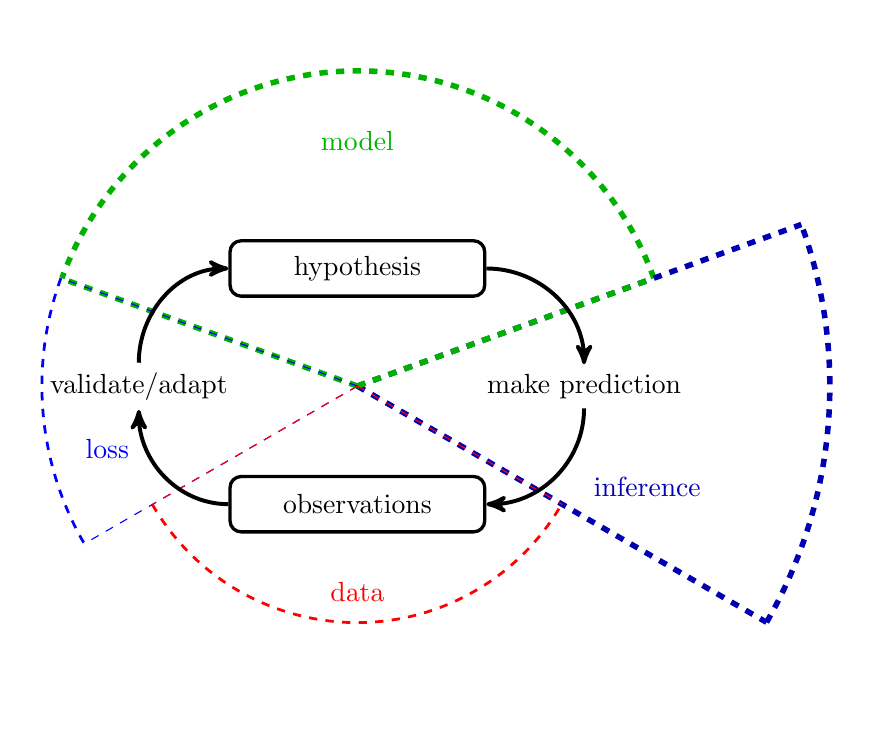
\begin{tikzpicture}[node distance=1cm, auto,]
	\coordinate (OR) at (0.00, 1.50);
	%\cercle {OR} {3cm} {-150} {120} {1.0} {red};
	\node[circle,inner sep=0,minimum size={6cm}](a) at (OR) {};
	\node[circle,inner sep=0,minimum size={8cm}](b) at (OR) {};
	\node[circle,inner sep=0,minimum size={8cm}](c) at (OR) {};
	\draw[red,line width=1,dashed] (a.-150) arc (-150:{-150+120}:3cm);
	\draw[blue,line width=1,dashed] (b.160) arc (160:{160+50}:4cm);
	\draw[black!30!green,line width=2,dashed] (c.20) arc (20:{160}:4cm);
	\draw[black!30!blue,line width=2,dashed] ([shift={(-30:6cm)}]OR) arc (-30:{20}:6cm);
	\draw[black!30!blue,line width=2,dashed] (OR) --([shift={(-30:6cm)}]OR);
	\draw[black!30!blue,line width=2,dashed] (OR) --([shift={(20:6cm)}]OR);
	\draw[black!30!green,line width=2,dashed] (OR) -- (c.20);
	\draw[black!30!green,line width=2,dashed] (OR) -- (c.160);
	\draw[blue,thin,dashed] (OR) -- (b.160);
	\draw[blue,thin,dashed] (OR) -- (b.210);
	\draw[red,thin,dashed] (OR) -- (a.-150);
	\draw[red,thin,dashed] (OR) -- (a.-30);   
	\node[punkt] (data) {observations};
	\node[red,below=0.5cm of data] (data1) {data};
	\node[above=of data] (dummy) {};
	\node[punkt,above=1cm of dummy] (hypothesis) {hypothesis};
	\node[right=1.4cm of dummy] (t) {make prediction} ; 
	\node[left=1.4cm of dummy] (g) {validate/adapt} ;
	\node[blue,below=0.5cm of g,anchor=east] (g1) {loss} ; 
	\node[black!30!blue,below=1cm of t,anchor=west] (g6) {inference} ; 
	\node[black!30!green,above=1cm of hypothesis,anchor=south] (g3) {model} ; 
	\draw [->,line width=0.5mm] (hypothesis.east) to [out=0,in=90] (t.north);
	\draw [->,line width=0.5mm] (t.south) to [out=270,in=0] (data.east);
	\draw [->,line width=0.5mm] (data.west) to [out=180,in=270] (g.south);
	\draw [->,line width=0.5mm] (g.north) to [out=90,in=180] (hypothesis.west);
	%   edge[pil, bend right=45] (data.west)
	%edge[pil, bend right=45] (formidler.west)
	%  edge[pil,<->, bend left=45] node[auto] {Direct (a)} (t)
	\end{tikzpicture}
	\vspace*{-9mm}
	\caption{
		Machine learning combines three main components: data, model and loss. Machine learning 
		methods implement the scientific principle of ``trial and error''. These methods continuously validate and 
		refine a model based on the loss incurred by its predictions about a phenomenon that generates data.}
	\label{fig_AlexMLBP}
\end{figure}
\end{center}



\newpage
\chapter*{Preface}

Machine learning (ML) has become a commodity in our every-day lives. 
We routinely ask ML empowered smartphones to suggest lovely food 
places or to guide us through a strange place. ML methods have also 
become standard tools in many fields of science and engineering. A 
plethora of ML applications transform human lives at unprecedented 
pace and scale. 

This book portrays ML as the combination of three basic components: 
data, model and loss. ML methods combine these three components 
within computationally efficient implementations of the basic scientific 
principle ``trial and error''. This principle consists of the continuous 
adaptation of a hypothesis about a phenomenon that generates data. 

ML methods use a hypothesis to compute predictions for future events. 
ML methods choose or learn a hypothesis from a (typically very) large set 
of candidate hypotheses. We refer to this set as candidates as the model 
of a ML method. 

The adaptation or improvement of the hypothesis is based on the discrepancy 
between predictions and observed data. ML methods use a loss function 
to quantify this discrepancy.

A plethora of different ML methods is obtained by combining different design 
choices for the data representation, model and loss. ML methods also differ 
vastly in their actual implementations which might obscure their unifying 
basic principles. 

Deep learning methods use cloud computing frameworks to train large 
models on huge datasets. Operating on a much finer granularity for 
data and computation, linear least squares regression can be implemented 
on small embedded systems. Nevertheless, deep learning methods and 
linear regression use the same principle of iteratively updating a model 
based on the discrepancy between model predictions and actual observed 
data. 

Our three-component picture of ML allows a unified treatment of a 
wide range of concepts and techniques which seem quite unrelated 
at first sight. On a low-level, we discuss the regularization effect of 
early stopping in terms of adjusting the effective model space. On a 
higher-level, we can interpret privacy-preserving and explainable ML as 
particular design choices for the model, data and loss. 

To make good use of ML tools it is instrumental to understand 
its underlying principles at different levels of detail. On a lower-level, 
this tutorial helps ML engineers to choose suitable methods for 
the application at hand. The book also provides leaders a 
higher-level view on the development of ML which is required 
to manage a ML or data analysis team. We believe that thinking 
about ML as combinations of data, model and loss helps to navigate 
the steadily growing offer for ready-to-use ML methods. 

\section*{Acknowledgement}
This tutorial is based on lecture notes prepared for the 
courses CS-E3210 ``Machine Learning: Basic Principles'', 
CS-E4800 ``Artificial Intelligence'', CS-EJ3211 ``Machine 
Learning with Python'', CS-EJ3311 ``Deep Learning with Python'' 
and CS-C3240 ``Machine Learning'' offered at Aalto 
University and within the Finnish university network 
\url{fitech.io}. This tutorial is accompanied by practical 
implementations of ML methods in MATLAB and 
Python \url{https://github.com/alexjungaalto/}. 

This text benefited from the numerous feedback of the 
students within the courses that have been (co-)taught 
by the author. The author is indebted to Shamsiiat Abdurakhmanova, 
Tomi Janhunen, Yu Tian, Natalia Vesselinova, Ekaterina Voskoboinik, 
Buse Atli, Stefan Mojsilovic for carefully reviewing early 
drafts of this tutorial. Some of the figures have been 
generated with the help of Eric Bach. The author is grateful 
for the feedback received from Jukka Suomela, V{\"a}in{\"o} Mehtola, 
Oleg Vlasovetc, Anni Niskanen, Georgios Karakasidis, Joni P{\"a}{\"a}kk{\"o}, 
Harri Wallenius and Satu Korhonen. 

%\end{abstract}

\tableofcontents                        % Print table of contents


\chapter{Introduction}
Consider waking up some morning during winter in Finland 
and looking outside the window (see Figure \ref{fig:skiday}). 
It seems to become a nice sunny day which is ideal for a 
ski trip. To choose the right gear (clothing, wax) it is 
vital to have some idea for the maximum daytime temperature 
which is typically reached around early afternoon. If we 
expect a maximum daytime temperature of around plus 
$10$ degrees, we might not put on the extra warm jacket 
but rather take only some extra shirt for change. 


\begin{figure}[htbp]
	\centering
	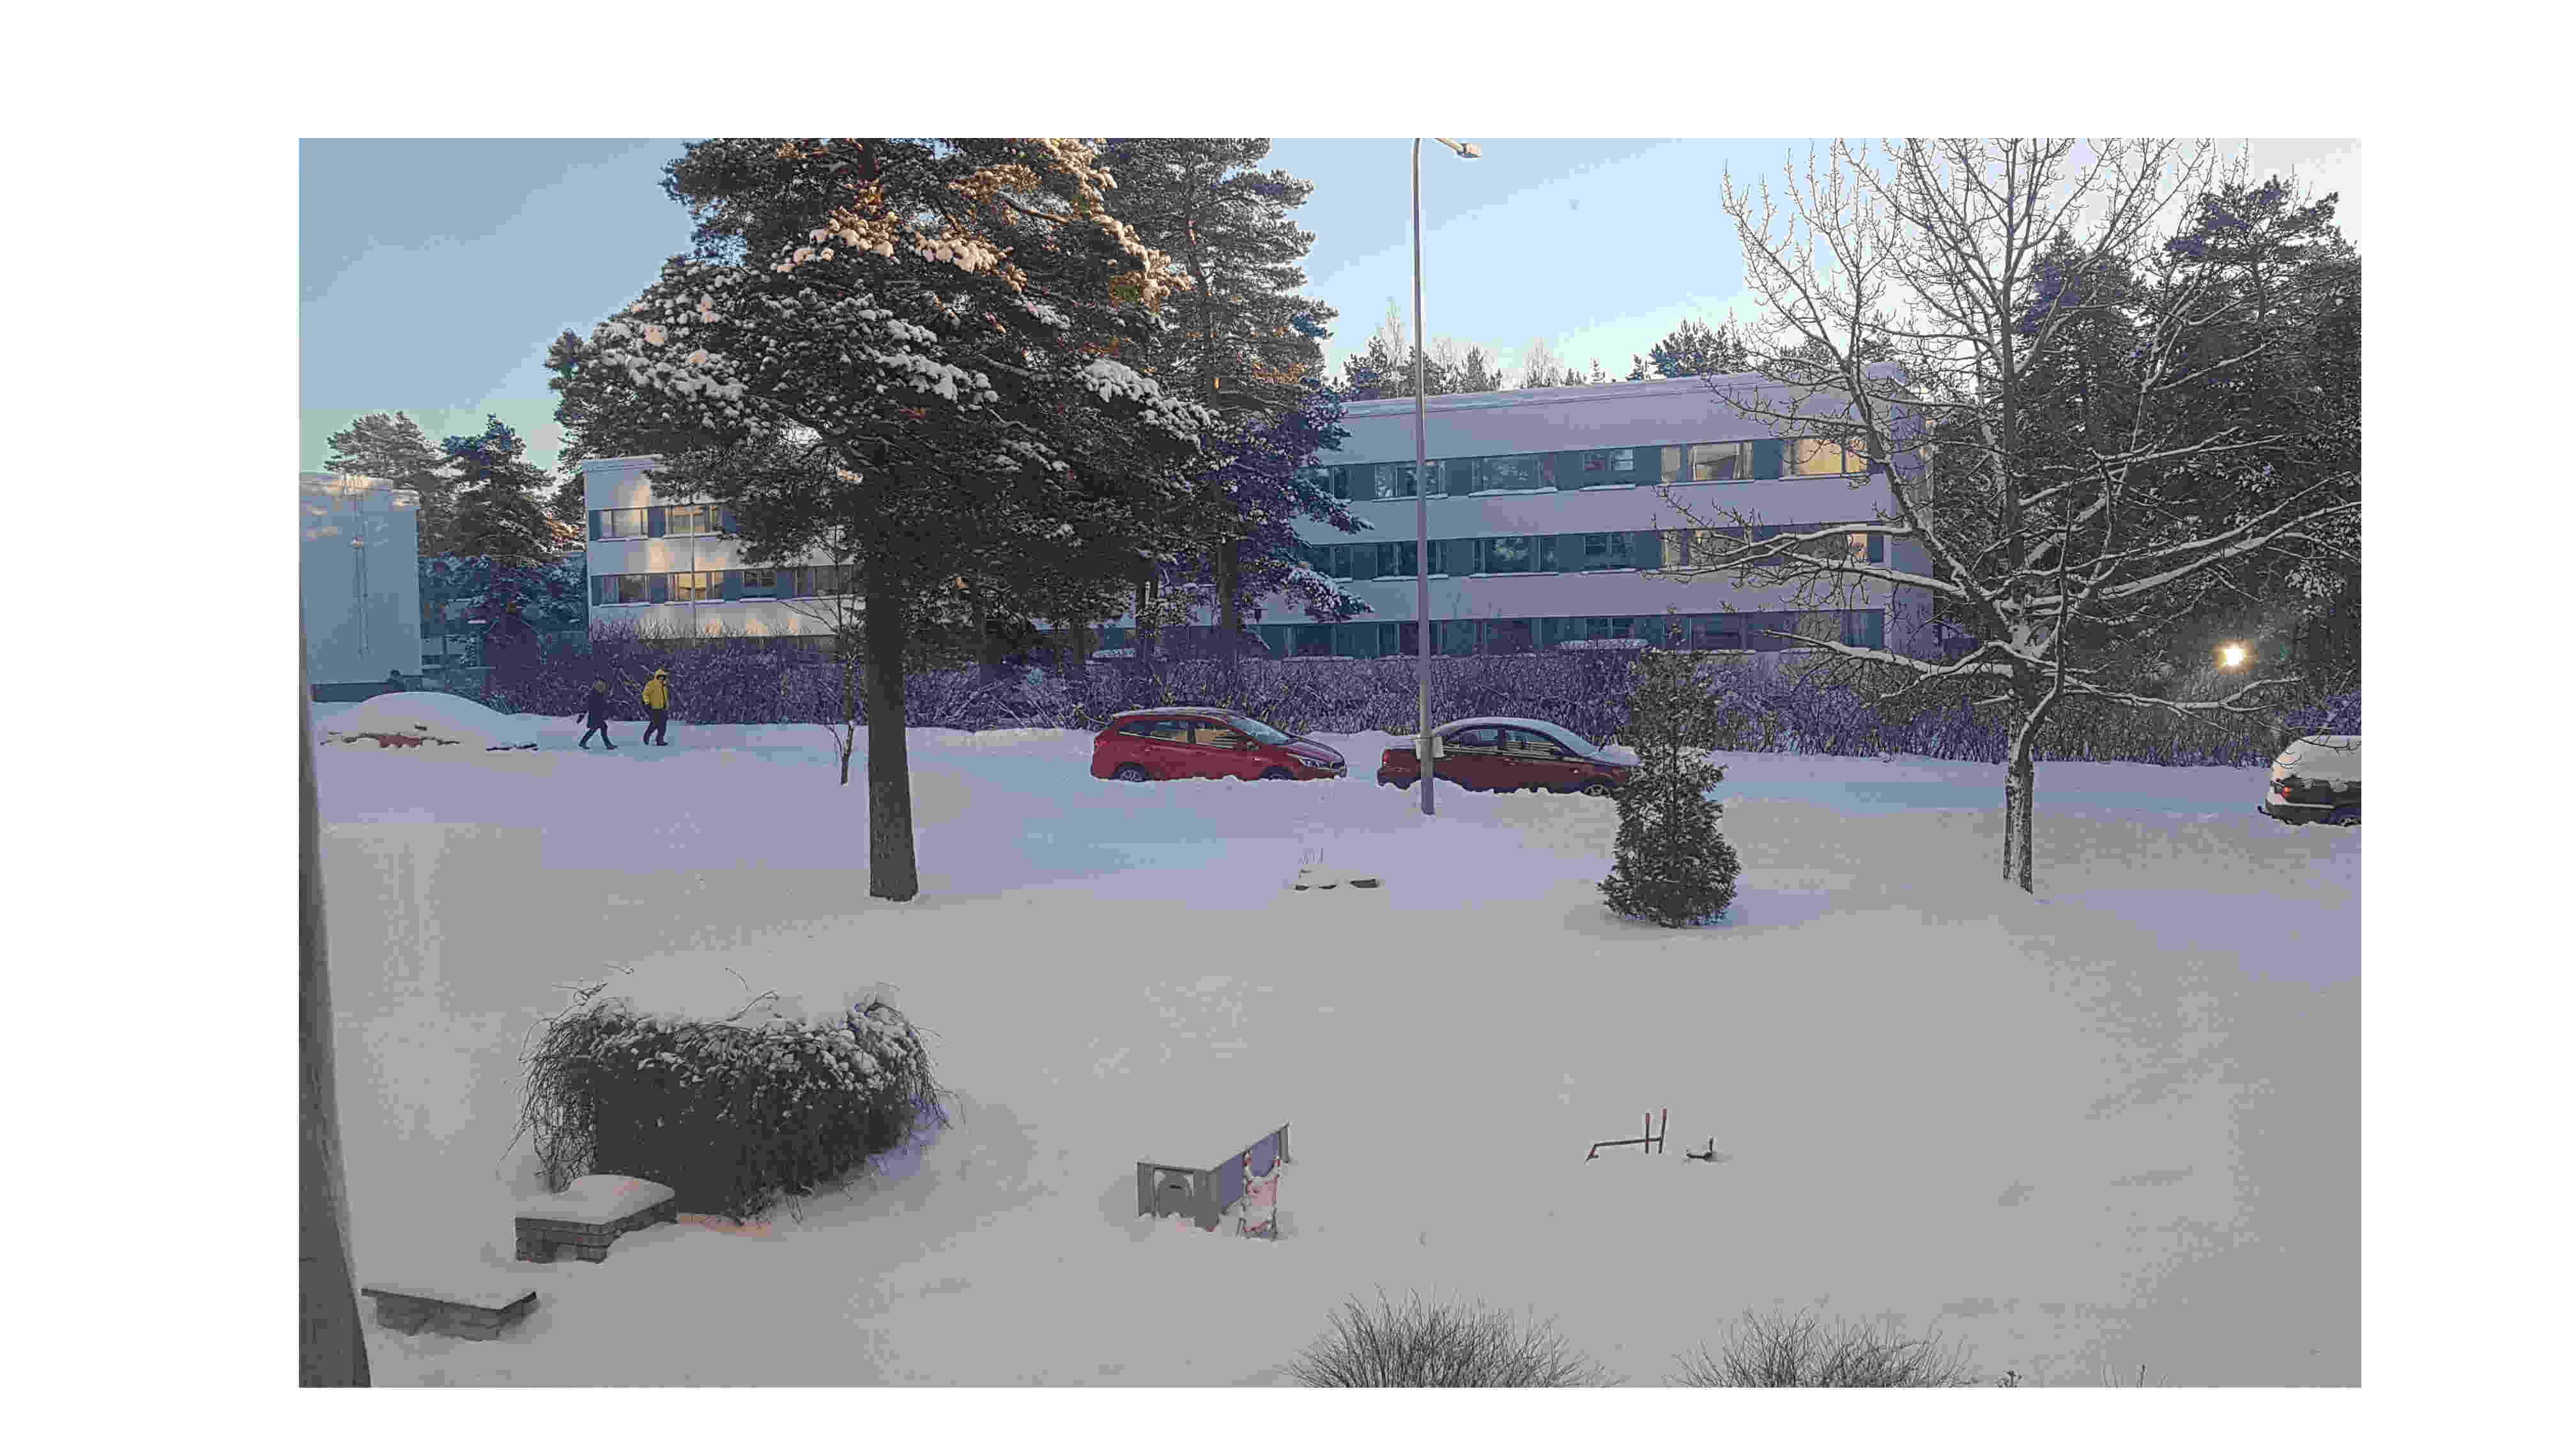
\includegraphics[width=8cm]{SkiDay2.jpeg}
	\caption{Looking outside the window during the morning of a winter day in Finland.}
	\label{fig:skiday}
\end{figure}

How can we predict the maximum daytime temperature for 
the specific day depicted in Figure \ref{fig:skiday}? Let us now 
show how this can be done via ML. In a nutshell, 
ML methods are computational implementations of a simple 
(scientific) principle. 

\begin{quote}
Find a good hypothesis based on {\bf a model} for the phenomenon of interest by 
using {\bf observed data} in order to minimize {\bf a loss function}. 
\end{quote}

This principle contains three components: data, a model and a 
loss function. Any ML method, including linear 
regression and deep reinforcement learning, combines these 
three components.  

We illustrate the (rather abstract) concepts behind the main 
components of ML with the above problem of predicting the 
maximum daytime temperature during some day in Finland (see Figure \ref{fig:skiday}). 
The prediction shall be based solely on the minimum daytime 
temperature observed in the morning of that day. 

The {\bf Finnish Meteorological Institute (FMI)} offers data 
on historic weather observations. We can download historic 
recordings of minimum and maximum daytime temperature 
recorded by some FMI weather station. Let us denote the 
resulting dataset by 
\begin{equation}
\label{equ_FMI_data}
\vz^{(1)},\ldots,\vz^{(\samplesize)}.  
\end{equation} 
Each datapoint $\vz^{(\sampleidx)} = \big(x^{(\sampleidx)},y^{(\sampleidx)}\big)$, 
for $\sampleidx=1,\ldots,\samplesize$, represents some previous 
day for which the minimum and maximum daytime temperature 
$x^{(i)}$ and $y^{(i)}$ has been recorded at some FMI station.  %We will use the minimum daytime temperature $x^{(i)}$ as the feature and the 
%maximum daytime temperature $y^{(i)}$ as the label of the datapoint $\vz^{(i)}$. 

We depict the data \eqref{equ_FMI_data} in Figure \ref{fig_scatterplot_temp_FMI}.  
Each dot in Figure \ref{fig_scatterplot_temp_FMI} represents a 
particular day which is characterized by the minimum daytime 
temperature $x$ and the maximum daytime temperature $y$. 

\begin{figure}[htbp]
	\begin{center}
		\begin{tikzpicture}
		\tikzset{x=0.35cm,y=2cm,every path/.style={>=latex},node style/.style={circle,draw}}
		%		\csvreader[ head to column names,%
		%		late after head=\xdef\iold{\maxtmp}\xdef\xold{\mintmp},,%
		%		after line=\xdef\iold{\maxtmp}\xdef\xold{\mintmp}]%
		%		{FMIData.csv}{}
		%		{\draw [line width=0.0mm] (\iold, \xold) (\i,\x) node {\large $\circ$};
		%		}
		%	
		\begin{axis}[axis x line=none,
		axis y line=none,
		ylabel near ticks,
		xlabel near ticks,
		enlarge y limits=true,
		xmin=-40, xmax=40,
		ymin=-40, ymax=40,
		width=10cm, height=10cm, ]
		\addplot[only marks] table [x=mintmp, y=maxtmp, col sep = comma] {FMIData.csv};
		\node at (axis cs:30,1) [anchor=west] {$x$};
		\node at (axis cs:0,30) [anchor=west] {$y$};
		\draw[->] (axis cs:-30,0) -- (axis cs:32,0);
		\draw[->] (axis cs:0,-30) -- (axis cs:0,30);
		\end{axis}
		\end{tikzpicture}
		\vspace*{-14mm}
	\end{center}
	\caption{Each dot represents a day that is characterized 
		by its minimum daytime temperature $x$ and its maximum 
		daytime temperature $y$ measured at some weather station in 
		Finland.}
	\label{fig_scatterplot_temp_FMI}
	\vspace*{-3mm}
\end{figure}

ML methods allow to learn a predictor map $h(x)$, reading in 
the minimum temperature $x$ and delivering a prediction (forecast or approximation) 
$\hat{y} = h(x)$ for the actual maximum daytime temperature $y$. 
We base this prediction on a simple hypothesis for how the minimum 
and maximum daytime temperature during some day are related. 
We assume that they are related approximately by 
\begin{equation}
\label{equ_initial_hypo_FMI}
y \approx w_{1} x + w_{0} \mbox{ with } w_{1} \geq 0. 
\end{equation}
This hypothesis reflects the intuition that the maximum daytime temperature 
$y$ should be higher for days with a higher minimum daytime temperature $x$. 

Given our initial hypothesis \eqref{equ_initial_hypo_FMI}, it seems reasonable 
to restrict the ML method to only consider linear predictor maps
\begin{equation} 
\label{equ_def_linear_map}
h(x) = w_{1} x + w_{0} \mbox{ with some weights } w_{1} \in \mathbb{R}_{+},w_{0} \in \mathbb{R}. 
\end{equation}
The map \eqref{equ_def_linear_map} is monotonically increasing since $w_{1}\!\geq\!0$. 

Note that \eqref{equ_def_linear_map} defines a whole ensemble of hypothesis maps, 
each individual map corresponding to a particular choice for $w_{1} \geq 0$ and $w_{0}$. 
We refer to such an ensemble of potential predictor maps as the {\bf model} or 
{\bf hypothesis space} of a ML method. 

We say that the map \eqref{equ_def_linear_map} is parameterized by the weight vector 
$\mathbf{w}= \big(w_{1},w_{0}\big)$ and indicate this by writing $h^{(\mathbf{w})}$. 
For a given weight vector $\mathbf{w}= \big(w_{1},w_{0}\big)$, we obtain the map 
$h^{(\mathbf{w})}(x) = w_{1}x +w_{0}$. 
Figure \ref{fig_three_maps_example} depicts three maps $h^{(\mathbf{w})}$ 
obtained for three different choices for the weights $\mathbf{w}$.  
\begin{figure}[htbp]
	\begin{center}
		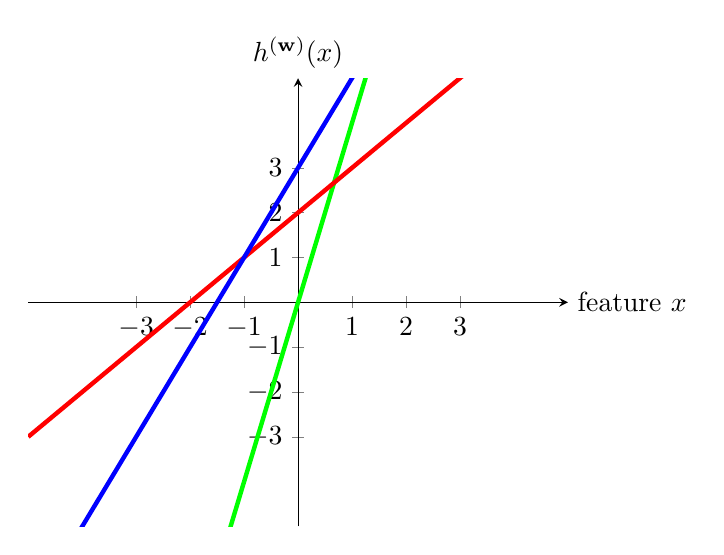
\begin{tikzpicture}
		\begin{axis}
		[ylabel=$h(x)$,
		xscale=1,
		xlabel=$x$, 
		axis x line=center,
		axis y line=center,
		xtick={-3,-2,-1,0,1,2,3},
		ytick={-3,-2,-1,0,1,2,3},
		xlabel={feature $x$},
		ylabel={$h^{(\mathbf{w})}(x)$},
		xlabel style={right},
		ylabel style={above},
		xmin=-5,
		xmax=5,
		ymin=-5,
		ymax=5
		]
		\addplot[green, ultra thick] (x,4*x);
		\addplot[red, ultra thick] (x,1*x+2);	
		\addplot[blue, ultra thick] (x,2*x+3);	
		%	\addplot [smooth, color=red, ultra thick] table [x=a, y=b, col sep=comma] {polynomials.csv};    
		%	\addplot [color=blue, ultra thick] table [x=a, y=c, col sep=comma] {polynomials.csv};     
		%	\addplot [color=black, thick] table [x=a, y=d, col sep=comma] {polynomials.csv};      
		\end{axis}
		%	\node [right,color=red] at (5.5,1.5) {$h^{(\mathbf{w}_{1})}(x) = 7(x^2 - x^3)$};
		%		\node [right,color=blue] at (2.3,0.5) {$h^{(\mathbf{w}_{2})}(x) =x^2$};
		%		\node [right] at (2.5,2.8) {$h^{(\mathbf{w}_{3})}(x)\!=\!x$};
		\end{tikzpicture}
		\vspace*{-4mm}
	\end{center}
	\caption{Three hypothesis maps of the form \eqref{equ_def_linear_map}.}
	\label{fig_three_maps_example}
\end{figure}

ML would be trivial if there is only one single hypothesis. Having 
only a single hypothesis means that there is no need to try out 
different hypotheses to find the best one. To enable ML, we need 
to choose between a whole space of different hypotheses. ML 
methods are computationally efficient methods to choose (learn) 
a good hypothesis out of (typically very large) hypothesis spaces. 
The hypothesis space constituted by the maps \eqref{equ_def_linear_map} 
for different weights is uncountably infinite. 

To find, or {\bf learn}, a good hypothesis out of the infinite 
set \eqref{equ_def_linear_map}, we need to somehow assess 
the quality of a particular hypothesis map. ML methods use 
data and a loss function for this purpose. 

A loss function is a measure for the difference between the actual 
data and the predictions obtained from a hypothesis map (see Figure \ref{fig_scatterplot_temp_FMI_linalg}). 
One widely-used example of a loss function is the squared error loss $(y-h(x))^2$. 
Using this loss function, ML methods learn a hypothesis map 
out of the model \eqref{equ_def_linear_map} by tuning $w_{1},w_{0}$ to minimize 
the average loss $$(1/\samplesize) \sum_{\sampleidx=1}^{\samplesize} \big( y^{(\sampleidx)} - h\big(x^{(\sampleidx)} \big) \big)^{2}.$$

\begin{figure}[htbp]
	\begin{center}
		\begin{tikzpicture}
		\tikzset{x=0.35cm,y=2cm,every path/.style={>=latex},node style/.style={circle,draw}}
		%		\csvreader[ head to column names,%
		%		late after head=\xdef\iold{\maxtmp}\xdef\xold{\mintmp},,%
		%		after line=\xdef\iold{\maxtmp}\xdef\xold{\mintmp}]%
		%		{FMIData.csv}{}
		%		{\draw [line width=0.0mm] (\iold, \xold) (\i,\x) node {\large $\circ$};
		%		}
		%	
		\begin{axis}[axis x line=none,
		axis y line=none,
		ylabel near ticks,
		xlabel near ticks,
		enlarge y limits=true,
		xmin=-40, xmax=40,
		ymin=-40, ymax=40,
		width=10cm, height=10cm, ]
		\addplot[only marks] table [x=mintmp, y=maxtmp, col sep = comma] {FMIData.csv};
		\node at (axis cs:30,1) [anchor=west] {$x$};
		\node at (axis cs:0,30) [anchor=west] {$y$};
		\draw[->] (axis cs:-30,0) -- (axis cs:32,0);
		\draw[->] (axis cs:0,-30) -- (axis cs:0,30);
		\draw[red,line width=3] (axis cs:-30,-10) -- (axis cs:20,25);
		%	\draw [red,rotate=40,thick] \boundellipse{axis cs:10,-36}{300}{50} node[left,xshift=3mm,yshift=10mm]  {$\,\,p(\vz)$}; 
		%	\fill (axis cs:0,0) circle (2pt) ; 
		%	\node [right] at (axis cs:-9,8) {$ {\bm \Sigma}^{(3)}$} ; 
		\end{axis}
		\end{tikzpicture}
		\vspace*{-14mm}
	\end{center}
	\caption{Dots represent days characterized by its minimum daytime temperature $x$ 
		and its maximum daytime temperature $y$. We also depict a straight line representing 
		a linear predictor map. ML methods learn a predictor map with minimum discrepancy 
		between predictor map and datapoints. 
	}
	\label{fig_scatterplot_temp_FMI_linalg}
	\vspace*{-3mm}
\end{figure}



%??? Work out this prinicple for linear regression using FMI data pionts ???

The above weather prediction is prototypical for many other 
ML applications. Figure \ref{fig_AlexMLBP} illustrates the typical 
workflow of a ML method. Starting from some initial guess, ML 
methods repeatedly improve their current hypothesis based on 
(new) observed data. 

Using the current hypothesis, ML methods make predictions or 
forecasts about future observations. The discrepancy between 
the predictions and the actual observations, as measured using 
some loss function, is used to improve 
the hypothesis. Learning happens during improving the current 
hypothesis based on the discrepancy between its predictions 
and the actual observations. 

ML methods must start with some initial guess or choice for a 
good hypothesis. This initial guess can be based on some prior 
knowledge or domain expertise \cite{MitchellBias1980}. While 
the initial guess for a hypothesis might not be made explicit in 
some ML methods, each method must use such an initial guess. 
In our weather prediction application discussed above, we 
used the approximate linear model \eqref{equ_initial_hypo_FMI} 
as the initial hypothesis. 
 
%A prominent example of a phenomenon is the weather. Forecasting the weather is 
%based on learning or fitting models to massive amounts of weather observations.  
%The Finnish Meteorological Institute collects weather measurements at different 
%observation stations distributed all over Finland. 


%In general we consider features being any property of a datapoint that can be 
%determined without human intervention. In contrast, labels are properties of 
%datapoints that require human expert knowledge or domain expertise. 

%Consider waking up on some day $i$. We can easily determine the minimum temperature 
%since this is what we can measure in the morning. However, we cannot easily determine 
%the maximum day temperature as this will be attained only a few hours later in 
%early afternoon. However, for this application we can get labeled datapoint, i.e., for 
%which we know the true label by using historic recordings. One main source for 
%labeled data is by looking into the past. 

%Machine learning (ML) uses data to learn models that allow, in turn, 
%to make predictions of forecasts. The models used in ML come in 
%the form of assumptions or hypothesis for the properties of observed 
%data. Consider the datapoint $\vz$ representing some day with minimum 
%temperature $x$ and maximum temperature $y$. Then, it seems reasonable 
%to assume that these two properties of the same day are correlated. 
%
%For a higher minimum temperature $x^{(i)}$, we typically expect a higher 
%maximum daytime temperature $y$. We can formalize this assumption by 
%modelling the maximum daytime temperature as $y \approx h(x)$ with some 
%hypothesis map $h$ which is monotonically increasing. One candidate for 
%such a map is a linear function of the form
%
%
%
%
%
%Consider the hypothesis map \eqref{equ_def_linear_map} for 
%predicting the maximum daytime temperature based on the 
%minimum (morning) daytime temperature $x$. We can evaluate 
%the quality of this map by comparing its predictions with actual 
%observed minimum and maximum temperature for previous days. 
%Figure \ref{fig_scatterplot_temp_FMI} depicts a set of datapoints 
%represented earlier days characterized by minimum and maximum 
%temperature. These datapoints can been downloaded from the 
%Finnish meteorological institute (FMI). 


\section{Relation to Other Fields}

ML builds on concepts from several other scientific fields. 

\subsection{Linear Algebra} 

Modern ML methods are computationally efficient methods to fit 
high-dimensional models to large amounts of data. The models 
underlying state-of-the-art ML methods can contain billions of 
tunable or learnable parameters. To make ML methods computationally 
efficient we need to use suitable representations for data and models. 

Maybe the most widely used mathematical structure to represent 
data is the Euclidean space $\mathbb{R}^{n}$ with some dimension 
$n$. The rich algebraic and geometric structure of $\mathbb{R}^{n}$ 
allows to design of ML algorithms that can process vast amounts 
of data to quickly update a model (parameters). 

The scatter plot in Figure \ref{fig_scatterplot_temp_FMI} depicts 
datapoints (individual days) using vectors $\vz \in \mathbb{R}^{2}$. 
We obtain a vector representation $\vz=(x,y)^{T}$ of a particular 
day by stacking the minimum daytime temperature $x$ and the 
maximum daytime temperature $y$ into a vector $\vz$ of 
length two. 

We can use the Euclidean space $\mathbb{R}^{n}$ not only to represent 
datapoints but also to represent models for the data. One such class of 
models is obtained by linear subsets of $\mathbb{R}^{n}$, such as those 
depicted in Figure \ref{fig_three_maps_example}. We can then use the geometric 
structure of $\mathbb{R}^{n}$, defined by the Euclidean norm, to search 
for the best model. As an example, we could search for the linear model, 
represented by a straight line, such that the average distance to the data 
points in Figure \ref{fig_scatterplot_temp_FMI} is as small as possible 
(see Figure \ref{fig_scatterplot_temp_FMI_linalg}). 

The properties of linear structures, such as straight lines, are 
studied within linear algebra \cite{StrangLinAlg2016}. The basic 
principles behind important ML methods, such as linear regression 
or principal component analysis, are deeply rooted in the theory 
of linear algebra (see Sections \ref{sec_lin_regression} and \ref{sec_pca}).

\subsection{Optimization} 

A main design principle for ML methods is to formulate learning tasks as  
optimization problems \cite{OptMLBook}. The weather prediction problem 
above can be formulated as the problem of optimizing (minimizing) the 
prediction error for the maximum daytime temperature.  ML methods are 
then obtained by applying optimization methods to these learning problems. 

The statistical and computational properties of such ML methods can be 
studied using tools from the theory of optimization. What sets the optimization 
problems arising in ML apart from ``standard'' optimization problems is that 
we do not have full access to the objective function to be minimized. 
Section \ref{ch_Optimization} discusses methods that are based on estimating 
the correct objective function by empirical averages that 
are computed over subsets of datapoints (the training set). 

\subsection{Theoretical Computer Science} 

On a high level, ML methods take data as input and compute 
predictions as their output. The predictions are computed 
using algorithms such as linear solvers or optimization methods. 
These algorithms are implemented using some finite computational 
infrastructure. 

One example for such a computational infrastructure is a single 
desktop computer. Another example for a computational infrastructure 
is an interconnected collection of computing nodes. ML methods 
must implement their computations within the available finite computational 
resources such as time, memory or communication bandwidth.  

%A main design principle within ML is to formulate learning tasks as an optimization problem. 
%ML methods are then obtained by applying optimization methods to these learning problems. 
Therefore, engineering efficient ML methods requires a good 
understanding of algorithm design and their implementation 
on physical hardware. A huge algorithmic toolbox is provided 
by numerical linear algebra \cite{StrangLinAlg2016,Strang2007}. 

The recent success of ML methods in several application domains 
might be attributed to their use of vectors and matrices to represent 
data and models. Using this representation allows to implement the 
resulting ML methods using highly efficient hard- and software 
implementations for numerical linear algebra. 


\subsection{Communication} 

We can interpret ML as a particular form of data processing. 
A ML algorithm is fed with observed data in order to adjust 
some model and, in turn, compute a prediction of some future 
event. Thus, ML involves transferring or communicating 
data to some computer which executes a ML algorithm. 

The design of efficient ML systems also involves the design 
of efficient communication between data source and ML algorithm. 
The learning progress of an ML method will be slowed down 
if it cannot be fed with data at sufficiently large rate. Given 
limited memory or storage capacity, being too slow to process 
data at their rate of arrival (in real-time) means that we need to 
``throw away'' data. The lost data might have carried relevant 
information for the ML task at hand. 



\subsection{Statistics}

%????? omit this ? ??????
%Many ML methods are based on statistical models for how data is generated. Once 
%such a statistical model is known or estimated, computing predictions amounts to 
%applying the calculus of probability theory. One important example for such a computation 
%is the Bayes rule which allows to compute the probability of a hidden variable (which 
%we want to predict) based on observed variables (the data we can feed into ML algorithms). 
%???????

Consider the datapoints depicted in Figure \ref{fig_scatterplot_temp_FMI}. 
Each datapoint represents some previous day. Each datapoint (day) 
is characterized by the minimum and maximum daytime temperature 
as measured by some weather observation station. It might 
be useful to interpret these datapoints as independent and 
identically distributed (i.i.d.) realizations of a random vector 
$\mathbf{z} =\big(x,y\big)^{T}$. The random vector $\vz$ 
is distributed according to some fixed but typically unknown 
probability distribution $p(\vz)$. Figure \ref{fig_scatterplot_temp_FMI_stat_model} 
extends the scatter plot of Figure \ref{fig_scatterplot_temp_FMI} 
with some contour line that indicates the probability distribution $p(\vz)$. 

%A simple but useful model for continuous-valued random vectors is provided by the  
%multivariate normal distribution. This distribution of parametrized by the mean vector 
%and the covariance matrix of the random vector. We can estimate the probability distribution 
%by estimating these two parameters based on the datapoints in Figure \ref{fig_scatterplot_temp_FMI}. 
Probability theory offers a great selection on methods for 
estimating the probability distribution from observed data 
(see Section \ref{sec_max_iikelihood}). Given (an estimate of) 
the probability distribution $p(\vz)$, we can compute estimates 
for the label of a datapoint based on its features. 

Having a probability distribution $p(\vz)$ for a randomly 
drawn datapoint $\vz=(x,y)$, allows us to not only compute 
a single prediction (point estimate) $\hat{y}$ of the label $y$ 
but rather an entire probability distribution $q(\hat{y})$ over 
all possible prediction values $\hat{y}$. 

The distribution $q(\hat{y}$) represents, for each value $\hat{y}$, 
the probability or how likely it is that this is the true label value of 
the datapoint. By its very definition, this distribution $q(\hat{y})$ 
is precisely the conditional probability distribution $p(y|x)$ of the 
label value $y$, given the feature value $x$ of a randomly drawn 
datapoint $\vz=(x,y) \sim p(\vz)$. 

Having an (estimate of) probability distribution $p(\vz)$ for the observed 
datapoints not only allows us to compute predictions but also to generate 
new datapoints. Indeed, we can artificially augment the available data  
by randomly drawing new datapoints according the probability distribution $p(\vz)$ 
(see Section \ref{sec_data_augmentation}). A recently popularized class of 
ML methods that use probabilistic models to generate synthetic data  
is known as {\bf generative adversarial networks} \cite{GoodfellowGAN}. 



\begin{figure}[htbp]
	\begin{center}
		\begin{tikzpicture}
		\tikzset{x=0.35cm,y=2cm,every path/.style={>=latex},node style/.style={circle,draw}}
		%		\csvreader[ head to column names,%
		%		late after head=\xdef\iold{\maxtmp}\xdef\xold{\mintmp},,%
		%		after line=\xdef\iold{\maxtmp}\xdef\xold{\mintmp}]%
		%		{FMIData.csv}{}
		%		{\draw [line width=0.0mm] (\iold, \xold) (\i,\x) node {\large $\circ$};
		%		}
		%	
		\begin{axis}[axis x line=none,
		axis y line=none,
		ylabel near ticks,
		xlabel near ticks,
		enlarge y limits=true,
		xmin=-40, xmax=40,
		ymin=-40, ymax=40,
		width=10cm, height=10cm, ]
		\addplot[only marks] table [x=mintmp, y=maxtmp, col sep = comma] {FMIData.csv};
		\node at (axis cs:30,1) [anchor=west] {$x$};
		\node at (axis cs:0,30) [anchor=west] {$y$};
		\draw[->] (axis cs:-30,0) -- (axis cs:32,0);
		\draw[->] (axis cs:0,-30) -- (axis cs:0,30);
	    \draw [red,rotate=40,thick] \boundellipse{axis cs:10,-36}{300}{50} node[left,xshift=3mm,yshift=10mm]  {$\,\,p(\vz)$}; 
	%	\fill (axis cs:0,0) circle (2pt) ; 
	%	\node [right] at (axis cs:-9,8) {$ {\bm \Sigma}^{(3)}$} ; 
		\end{axis}
		\end{tikzpicture}
		\vspace*{-14mm}
	\end{center}
	\caption{A scatterplot where each dot represents some day that is characterized 
		by its minimum daytime temperature $x$ and its maximum daytime temperature $y$.}
	\label{fig_scatterplot_temp_FMI_stat_model}
	\vspace*{-3mm}
\end{figure}




\subsection{Artificial Intelligence}

ML is instrumental for the design and analysis of artificial intelligence (AI). 
AI systems (hard and software) interacts with their environment by 
taking certain actions. These actions influence the environment as 
well as the state of the AI system. The behaviour of an AI system 
is determined by how the perceptions made about the environment 
are used to form the next action. 

From an engineering point of view, AI aims at optimizing behaviour to 
maximize a long-term {\bf return}. The optimization of behaviour is based 
solely on the perceptions made by the agent. Let us consider some 
application domains where AI systems can be used:
\begin{itemize}
\item a {\bf forest fire management system}: perceptions given by 
satellite images and local observations using sensors or ``crowd sensing'' 
via some mobile application which allows humans to notify about 
relevant events; actions amount to issuing warnings and bans of 
open fire; return is the reduction of number of forest fires. 
\item a {\bf control unit} for combustion engines: 
perceptions given by various measurements such as temperature, 
fuel consistency; actions amount to varying fuel feed and timing 
and the amount of recycled exhaust gas; return is measured in 
reduction of emissions.   
\item a {\bf severe weather warning service}: perceptions given by 
weather radar; actions are preventive measures taken by farmers or 
power grid operators; return is measured by savings in damage 
costs (see \url{https://www.munichre.com/})
\item an automated {\bf benefit application system} for a social 
insurance institute (like ``Kela'' in Finland): perceptions given by 
information about application and applicant; actions are either to 
accept or to reject the application along with a justification for the 
decision; return is measured in reduction of processing time 
(applicants tend to prefer getting decisions quickly)
\item  a {\bf personal diet assistant}: perceived environment is the 
food preferences of the app user and their health condition; actions 
amount to personalized suggestions for healthy and tasty food;  
return is the increase in well-being or the reduction in public spending 
for health-care.  
\item the {\bf cleaning robot} \rumba\, (see\ Figure \ref{fig:cleaning_robot}) 
perceives its environment using different sensors (distance sensors, 
on-board camera); actions amount to choosing different moving 
directions (``north'', ``south'', ``east'', ``west''); return might be the 
amount of cleaned floor area within a particular time period. 
\item {\bf personal health assistant:}  perceptions given by current 
health condition (blood values, weight,\ldots), lifestyle (preferred 
food, exercise plan);  actions amount to personalized suggestions 
for changing lifestyle habits (less meat, more jogging,\ldots); return 
is measured via the level of well-being (or the reduction in public 
spending for health-care).  
\item {\bf government-system} for a community: perceived environment 
is constituted by current economic and demographic indicators such as 
unemployment rate, budget deficit, age distribution,\ldots; actions involve 
the design of tax and employment laws, public investment in infrastructure, 
organization of health-care system; return might be determined by the 
gross domestic product, the budget deficit or the gross national 
happiness (cf. \url{https://en.wikipedia.org/wiki/Gross_National_Happiness}). 
\end{itemize}
	\vspace*{2mm}
\begin{figure}[htbp]
	\begin{center}
		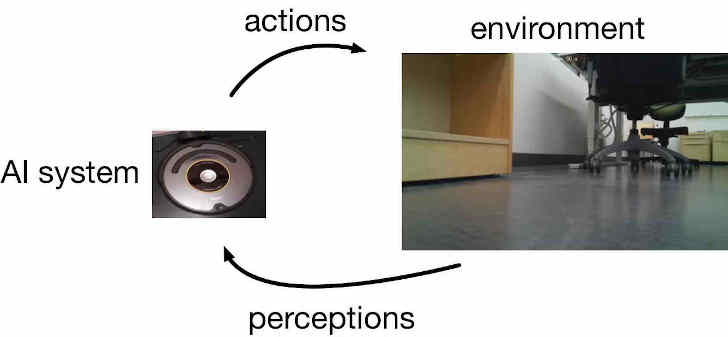
\includegraphics[width=8cm]{AIsystemEnvML1.jpg}  
		\caption{A cleaning robot chooses actions (moving directions) to maximize 
			a long-term reward measured by the amount of cleaned floor area per day.}
		\label{fig:cleaning_robot}
	\end{center}
\end{figure}

ML methods are used on different levels within AI systems. 
On a low-level, ML methods help to extract the relevant information 
from raw data. AI systems use  ML methods to classify images into 
different categories. The AI system subsequently only needs to process 
the category of the image instead of its raw digital form. 

ML methods are also used for higher-level tasks of an AI system. 
To behave optimally, an AI system or agent is required to learn a 
good hypothesis about how its behaviour affects its environment. 
We can think of optimal behaviour as the consequent choice of actions 
that are predicted as optimal according to some hypothesis which 
could be obtained by ML methods. 

%A widely used operation mode of ML is to predict some quantity of interest, or label, of 
%some datapoint based on some features. Such a datapoint could also represent some 
%situation which requires a decision. For example, a particular datapoint could correspond 
%to some driving situation of an autonomous car. We can use all the measurements provided 
%on-board sensors to predict the best steering angle as the quantity of interest (or label). 

What sets AI methods apart from other ML methods is that they must 
compute predictions in real-time while collecting data and choosing 
the next action. Consider an AI system that steers a toy car. In any 
given state (point of time) the resulting prediction influences immediately 
the features of the following datapoints. 

Consider datapoints that represent different states of a toy car. 
For such datapoints we  could define their labels as the optimal 
steering angle for these states. However, it might be very challenging 
to obtain accurate label values for any of these datapoints. Instead, 
we could evaluate the usefulness of a particular steering angle only 
in an indirect fashion by using a reward signal. For the toy car example, 
we might obtain a reward from a distance sensor that indicates if the 
car reduces the distance to some goal or target location. 


\section{Flavours of Machine Learning} 

The main focus of this tutorial is on {\bf supervised ML methods}. 
Supervised ML assigns labels to each datapoint. The label of a data 
points is some quantity of interest or higher-level fact. Roughly 
speaking, labels are properties of a datapoint that cannot be 
measured or computed easily. This is in contrast to features which 
are properties of datapoints that can be measured or computed 
easily (see Chapter \ref{sec_the_data}). 

{\bf Supervised Learning.} Supervised learning methods learn 
a (predictor or classifier) map that reads in features of a datapoint 
and outputs a prediction for its label (quantity of interest). The 
prediction should be an accurate approximation to the true label 
(see Chapter \ref{ch_Elements_ML}). To find such a map, supervised 
ML methods use labeled (training) data to try out different choices for 
the map.  

The basic idea of supervised ML methods, as illustrated in 
Figure \ref{fig_curve_fitting}, is to fit a curve (representing 
the predictor map) to datapoints obtained from historic data 
(see Chapter \ref{ch_Optimization}). While this sounds like a 
simple task, the challenge of modern ML applications is the sheer 
amount of datapoints. 

ML methods must process billions of datapoints with each 
single datapoint characterized by a potentially vast number 
of features. Consider datapoints representing social network 
users, whose features include all media that has been posted (videos, images, text). 

Besides the sheer size of datasets, another challenge 
in modern ML methods is that they must be able to fit 
highly non-linear predictor maps. Deep learning methods 
address this challenge by using a computationally convenient 
representation of non-linear maps via artificial neural networks \cite{Goodfellow-et-al-2016}. 


\begin{figure}[htbp]
	\begin{center}
		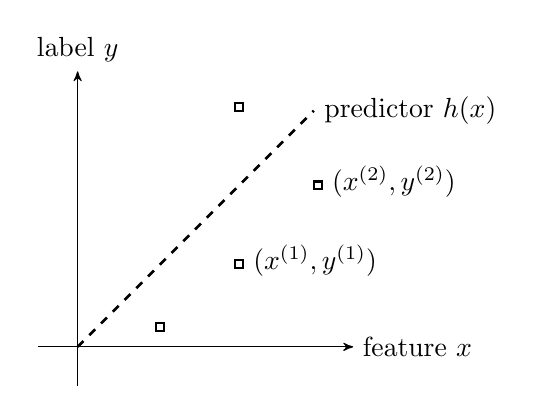
\begin{tikzpicture}[auto,scale=1]
		%\draw [thick] (5,2.5) circle (0.1cm)node[anchor=west] {\hspace*{0mm}$\vx^{(3)}$};
		%\draw [thick] (4,2) circle (0.1cm)node[anchor=west] {\hspace*{0mm}$\vx^{(4)}$};
		%\draw [thick] (5,1) circle (0.1cm)node[anchor=west,above] {\hspace*{0mm}$\vx^{(2)}$};
		\draw [thick] (1,0.2) rectangle ++(0.1cm,0.1cm) ;%node[anchor=west,above] {\hspace*{0mm}$\vx^{(1)}$};
		\draw [thick] (2,3) rectangle ++(0.1cm,0.1cm) ; %node[anchor=west,above] {\hspace*{0mm}$\vx^{(5)}$};
		\draw [thick] (3,2) rectangle ++(0.1cm,0.1cm) node[anchor=west] {\hspace*{0mm}$(x^{(2)},y^{(2)})$};%node[anchor=west,above] {\hspace*{0mm}$\vx^{(6)}$};
		\draw [thick] (2,1) rectangle ++(0.1cm,0.1cm) node[anchor=west] {\hspace*{0mm}$(x^{(1)},y^{(1)})$};
		\draw[->] (-0.5,0) -- (3.5,0) node[right] {feature $x$};
		\draw[dashed,line width=1pt] (0,0) -- (3,3) node[anchor=west] {predictor $h(x)$} ; 
		\draw[->] (0,-0.5) -- (0,3.5) node[above] {label $y$};
		%\foreach \y/\ytext in { 1/1,2/2,3/3,4/4,5/5} \draw[shift={(0,\y)}] (2pt,0pt) -- (-2pt,0pt) node[left] {$\ytext/5$};  
		%\foreach \x/\xtext in{ 1/1,2/2,3/3,4/4,5/5}\draw[shift={(\x,0)}] (0pt,2pt) -- (0pt,-2pt) node[below] {$\xtext/5$};  
		\end{tikzpicture}
	\end{center}
	\caption{Supervised ML methods fit a curve to (a huge number of) datapoints. 
	} 
	\label{fig_curve_fitting}
\end{figure}

{\bf Unsupervised Learning.}
Some ML applications do not need the concept of labels 
but require only to understand the intrinsic structure of data 
points. We refer to such applications as {\bf unsupervised ML.} 
One important example for an intrinsic structure of a dataset is 
when its datapoints can be grouped into a few coherent subsets 
of cluster (see Chapter \ref{ch_Clustering}). Another example for 
such an intrinsic structure is when the datapoints are localized 
around a low-dimensional subspace (see Chapter \ref{ch_FeatureLearning}). 
Unsupervised ML methods allow to determine such an intrinsic structure. 

{\bf Reinforcement Learning.} 
Another main flavour of ML considers datapoints that are characterized 
by labels but which cannot be determined easily beforehand. Reinforcement 
learning studies applications where the label values can only be determined 
in an indirect fashion. Consider the problem of predicting the next optimal 
moving direction for a toy car given its current state. datapoints represent 
a particular state of the car, its label is the optimum steering direction. 

It is typically impossible to get labeled datapoints here since there 
are so many different driving scenarios that each have a different 
optimal steering direction. Instead, RL methods must try out 
some predictor of the optimal steering direction and then 
evaluate the quality of this prediction by some feedback signal. 
Such a feedback signal might be obtained from GPS sensors that 
allow to determine if the car stays in the lane. 

\section{Organization of this Book}

Chapter \ref{ch_Elements_ML} introduces the concepts of data, 
model and loss function as main components of ML. We also 
highlight that each component involves design choices that must 
take into account computational and statistical aspects. 
%the design choices incurred 
%by the ML components data, model and loss. These design choices 
%include the representation for data and  models. %One such choice for 
%data and model representation is to use vectors and matrices. 

Chapter \ref{ch_some_examples} shows how well-known ML methods 
are obtained by specific design choices for the data, model
and loss function. The aim of this chapter is to organize ML methods 
according to three dimensions representing data, model and loss. 

Chapter \ref{ch_Optimization} explains how a simple probabilistic 
model for data lends to the principle of {\bf empirical risk minimization (ERM)}. 
This principle translates the problem of learning into an optimization problem. 
ML methods based on the ERM are therefore a special class of 
optimization methods. The ERM principle can be interpreted as 
a precise mathematical formulation of the ``learning by trial and error'' paradigm. 

Chapter \ref{ch_GD} discusses a powerful principle for learning 
predictors with a good performance. This principle uses the concept 
of gradients to locally approximate an objective function used 
to score predictors. A basic implementation of gradient-based 
optimization is the gradient descent (GD) algorithm. Variations 
of GD are currently the de-facto standard method for training 
deep neural networks \cite{Goodfellow-et-al-2016}. 

Chapter \ref{ch_validation_selection} discusses one of the most 
important ideas in applied ML. This idea is to validate a predictor 
by trying it out on validation or test data which is different from 
the training data that has been used to fit a model to data. As 
detailed in Chapter \ref{ch_overfitting_regularization}, a main 
reason for doing validation is to detect and avoid {\bf overfitting} 
which is a main reason for ML methods to fail. 

%In some ML applications there is no reason for defining labels associated with datapoints. 
%The resulting ML methods are then called {\bf unsupervised ML methods}. 
Chapter \ref{ch_Clustering} presents some basic methods for {\bf clustering} 
data. These methods group or partition datapoints into 
coherent groups which are referred to as clusters. 

The efficiency of ML methods often depends crucially on the choice 
of data representation. Ideally we would like to have a small number 
of highly relevant features to characterize datapoints. If we use too 
many features we risk to waste computations on exploring irrelevant 
features. If we use too few features we might not have enough information 
to predict the label of a datapoint. Chapter \ref{ch_FeatureLearning} 
discusses {\bf feature learning} methods that automatically determine 
the most relevant features from the ``raw features'' of a datapoint. 

%These methods exploit 
%intrinsic correlations and redundancy in the raw data to construct 
%few relevant features for datapoints. These relevant features can 
%be subsets of raw features (feature selection) or combinations 
%of all raw features (feature transformation). 

Two main challenges for the widespread use of ML techniques 
in critical application domains is privacy-preservation and 
explainability. Chapters \ref{chap_privacy_preserving_ML} 
and \ref{chap_explainable_ML} will discuss recent approaches 
to solve these challenges. We will see that the concepts 
developed in Chapter \ref{ch_FeatureLearning} for feature 
learning will be perfect tools for {\bf privacy-preserving and 
explainable ML}. 

{\bf Prerequisites.} We assume some familiarity with basic concepts 
of linear algebra, real analysis, and probability theory. For a review of 
those concepts, we recommend \cite[Chapter 2-4]{Goodfellow-et-al-2016} 
and the references therein. 

{\bf Notation.} We mainly follow the notational conventions used 
in \cite{Goodfellow-et-al-2016}. Boldface upper case letters such 
as $\mA,\mX,\ldots$ denote matrices. Boldface lower case letters 
such as $\vy,\vx,\ldots$) denote vectors. The generalized identity 
matrix $\mathbf{I}_{\featuredim \times r} \in \{0,1\}^{\featuredim \times r}$ 
is a diagonal matrix with ones on the main diagonal. The Euclidean 
norm of a vector $\vx=(x_{1},\ldots,x_{\featuredim})^{T}$ is denoted 
$\| \vx \| = \sqrt{ \sum_{r=1}^{\featuredim} x^{2}_{r}}$. 

\newpage
\chapter{Three Components of ML: Data, Model and Loss} 
\label{ch_Elements_ML}

\begin{figure}[htbp]
	\begin{center}
		\tikzset{pics/.cd,
			jigsaw/.style={
				code={
					\fill[#1] (-2,-0.35) to[out=90,in=135] (-1.5,-0.45) arc(-135:135:0.6 and
					{0.45*sqrt(2)}) to[out=-135,in=-90] (-2,0.35) |- (-0.35,2)
					to[out=0,in=-45] (-0.45,2.5) arc(225:-45:{0.45*sqrt(2)} and 0.6)
					to[out=-135,in=180] (0.35,2) -| (2,0.35) 
					to[out=-90,in=225] (2.5,0.45) arc(135:-135:0.6 and {0.45*sqrt(2)})
					to[out=135,in=90] (2,-0.35) |- (0.35,-2)
					to[out=180,in=-135] (0.45,-1.5) arc(-45:225:{0.45*sqrt(2)} and 0.6) 
					to[out=-45,in=0] (-0.35,-2) -| cycle;
		}}}
		
		\resizebox{5cm}{!}{
			\begin{tikzpicture}
			\draw (-2,-2) pic{jigsaw=white!80!blue} (2,-2) pic{jigsaw=white!80!green}
			%(-2,2) pic[rotate=90]{jigsaw=purple}
			(2,2) pic[rotate=90]{jigsaw=white!80!red};
			\node[anchor=west] at (0.4,3.1) {\bf\Huge model};
			\node[anchor=west] at (0.4,-0.9) {\bf\Huge loss};
			\node[anchor=west] at (-2.4,-0.9) {\bf\Huge data};
			\end{tikzpicture}}
	\end{center} 
	\caption{ML methods fit a model to data via minimizing a loss function.}
	\label{fig_ml_problem}
\end{figure}

%Consider the cleaning robot ``\rumba'' in Figure \ref{fig:rumba}, which has to clean the office room B329. 
%For simplicity, we model this office room as a plain rectangular area (see Figure \ref{fig:RoomGridworld}) in what follows. 
%We discretise the office floor using small squares or ``cells''. A particular cell within room B329 is represented by the 
%coordinate pair $\gridcell{m}{y}$ with coordinates $m \in \{1,\ldots,\gridsizex\}$ and $y \in \{1,\ldots,\gridsizey\}$. 
%\begin{figure}[htbp]
%	\centering
%	\includegraphics[width=8cm]{Rumba_Charging0.jpg}
%	\caption{The cleaning robot ``\rumba''.}
%	\label{fig:rumba}
%\end{figure}
%
%\begin{figure}[htbp]
%	\centering
%	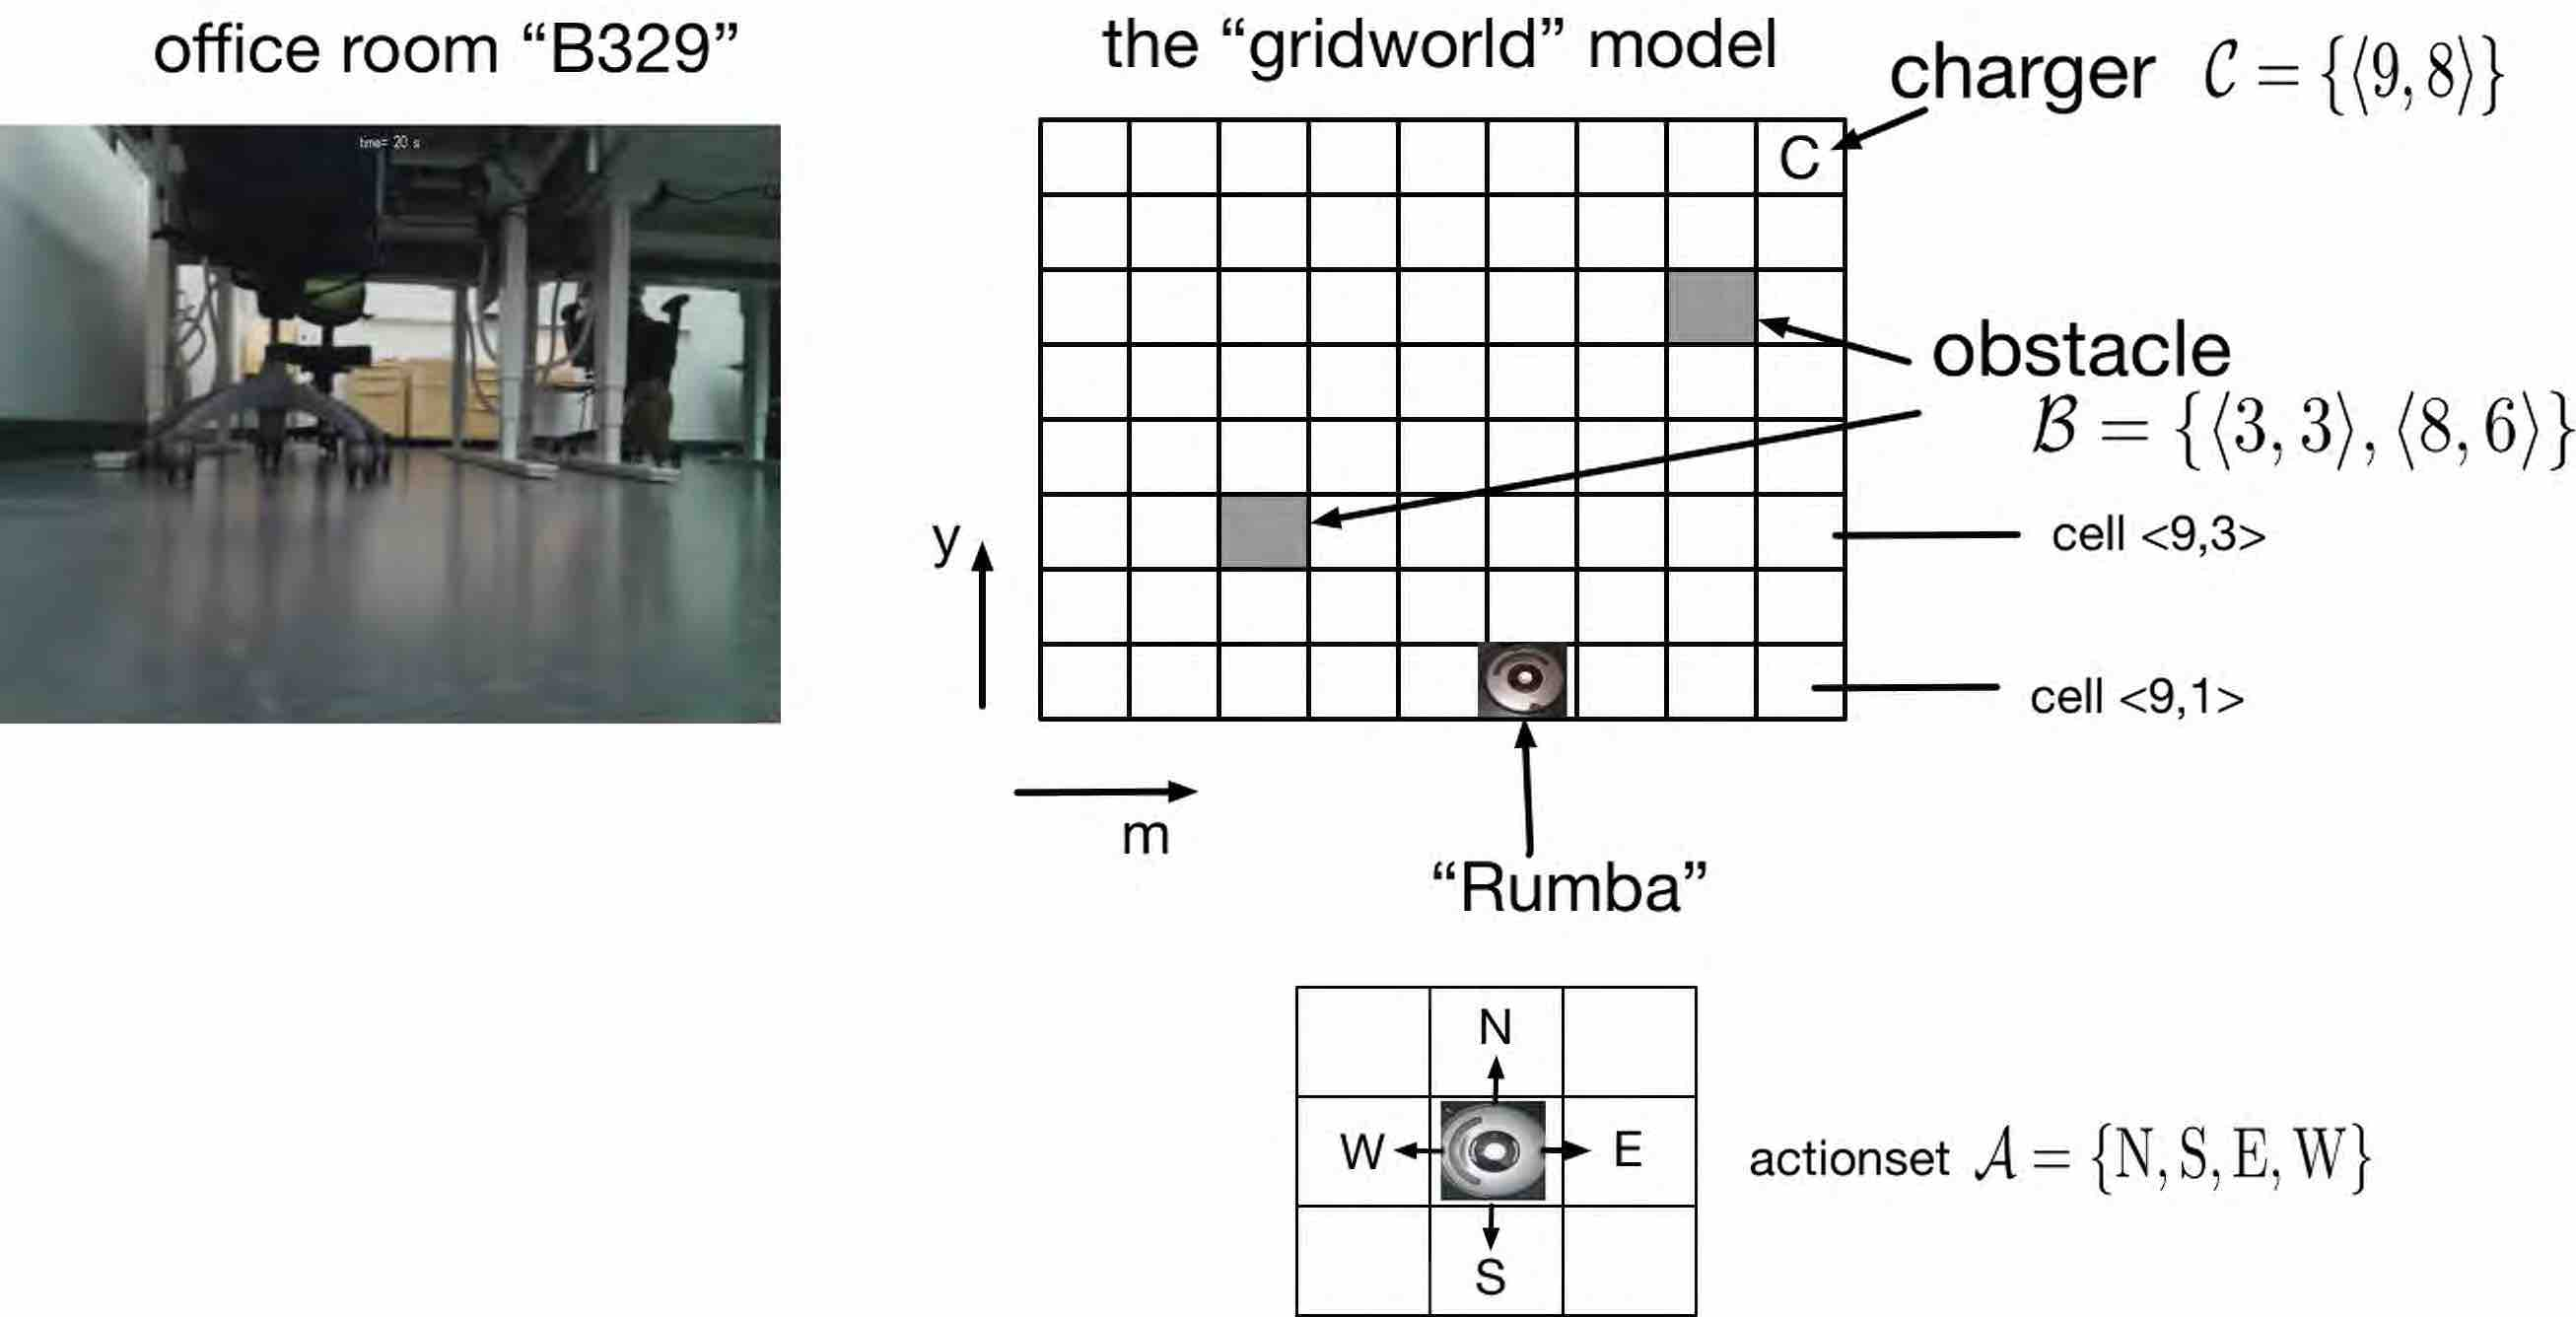
\includegraphics[width=\textwidth]{RoomGridworld.jpg}
%	\caption{The office room which \rumba\, has to keep tidy, and a simple gridworld model of the room's floor space. 
%	We also depict the action set of Rumba, which is constituted by the four compass direction into which the cleaning robot can move.}
%	\label{fig:RoomGridworld}
%\end{figure}
%
%From time to time, \rumba\, has to visit a charging station in order to charge its battery.
%In order to reach a charging station, \rumba\, can choose from different actions each of which 
%corresponding to a particular direction into which it can move next (see Figure \ref{fig:RoomGridworld}). 
%The optimal action at a particular time $\timeidx$ depends on the current location $\gridcell{m_{\timeidx}}{y_{\timeidx}}$ of \rumba. 
%However, it turns out that determining the precise location within a typical office room is far from trivial 
%(see \url{http://www.indooratlas.com/how-it-works/}).Therefore, let us now assume that \rumba\, has to predict 
%(or infer) its location, i.e., the coordinates $m_{\timeidx}$ and $y_{\timeidx}$, using solely the 
%information contained in the snapshots generated by some on-board camera. We also depict the 
%action set of Rumba, which is constituted by the four compass direction into which the cleaning 
%robot can move. 
%
This book portrays ML as combinations of three components: 
\begin{itemize}
	\item {\bf data} as collections of datapoints characterized by 
	{\bf features} (see Section \ref{sec_feature_space}) and {\bf labels} 
	(see Section \ref{sec_labels}) 
	\item a {\bf model} or {\bf hypothesis space} (see Section \ref{sec_hypo_space}) 
	of computationally feasible maps (called ``predictors'' or ``classifiers'') 
	from feature to label space 
	\item a {\bf loss function} (see Section \ref{sec_lossfct}) to measure 
	the quality of a predictor (or classifier). 
\end{itemize}
We formalize a ML problem or application by identifying these three 
components for a given application. A formal ML problem is obtained 
by specific design choices for how to represent data, which hypothesis 
space or model to use and with which loss function to measure the 
quality of a hypothesis. Once the ML problem is formally defined, 
we can readily apply off-the-shelf ML methods to solve them. 

Similar to ML problems (or applications) we also think of ML 
methods as specific combinations of the three above components. 
We detail in Chapter \ref{ch_some_examples} how some of the 
most popular ML methods, such as linear regression and deep 
learning methods, are obtained by specific design choices for 
the three components. 

Linear regression is a ML method which uses linear maps for 
the hypothesis space and the squared error loss function. 
Deep learning methods are characterized by using artificial 
neural networks to represent hypothesis spaces constituted 
by highly non-linear predictor maps. The remainder of this 
chapter discusses in some depth each of the three main 
components of ML. 





\section{The Data}
\label{sec_the_data}

{\bf Data as Collections of datapoints.} Maybe the most important 
component of any ML problem (and method) is data. We consider 
data as collections of individual datapoints which are atomic units 
of ``information containers''. datapoints can represent text documents, 
signal samples of time series generated by sensors, entire time series 
generated by collections of sensors, frames within a single video, 
videos within a movie database, cows within a herd, trees within a 
forest, forests within a collection of forests. Consider the problem 
of predicting the duration of a mountain hike (see Figure \ref{fig:image}). 
Here, datapoints could represent different hiking tours.  

\begin{figure}[htbp]
	\centering
	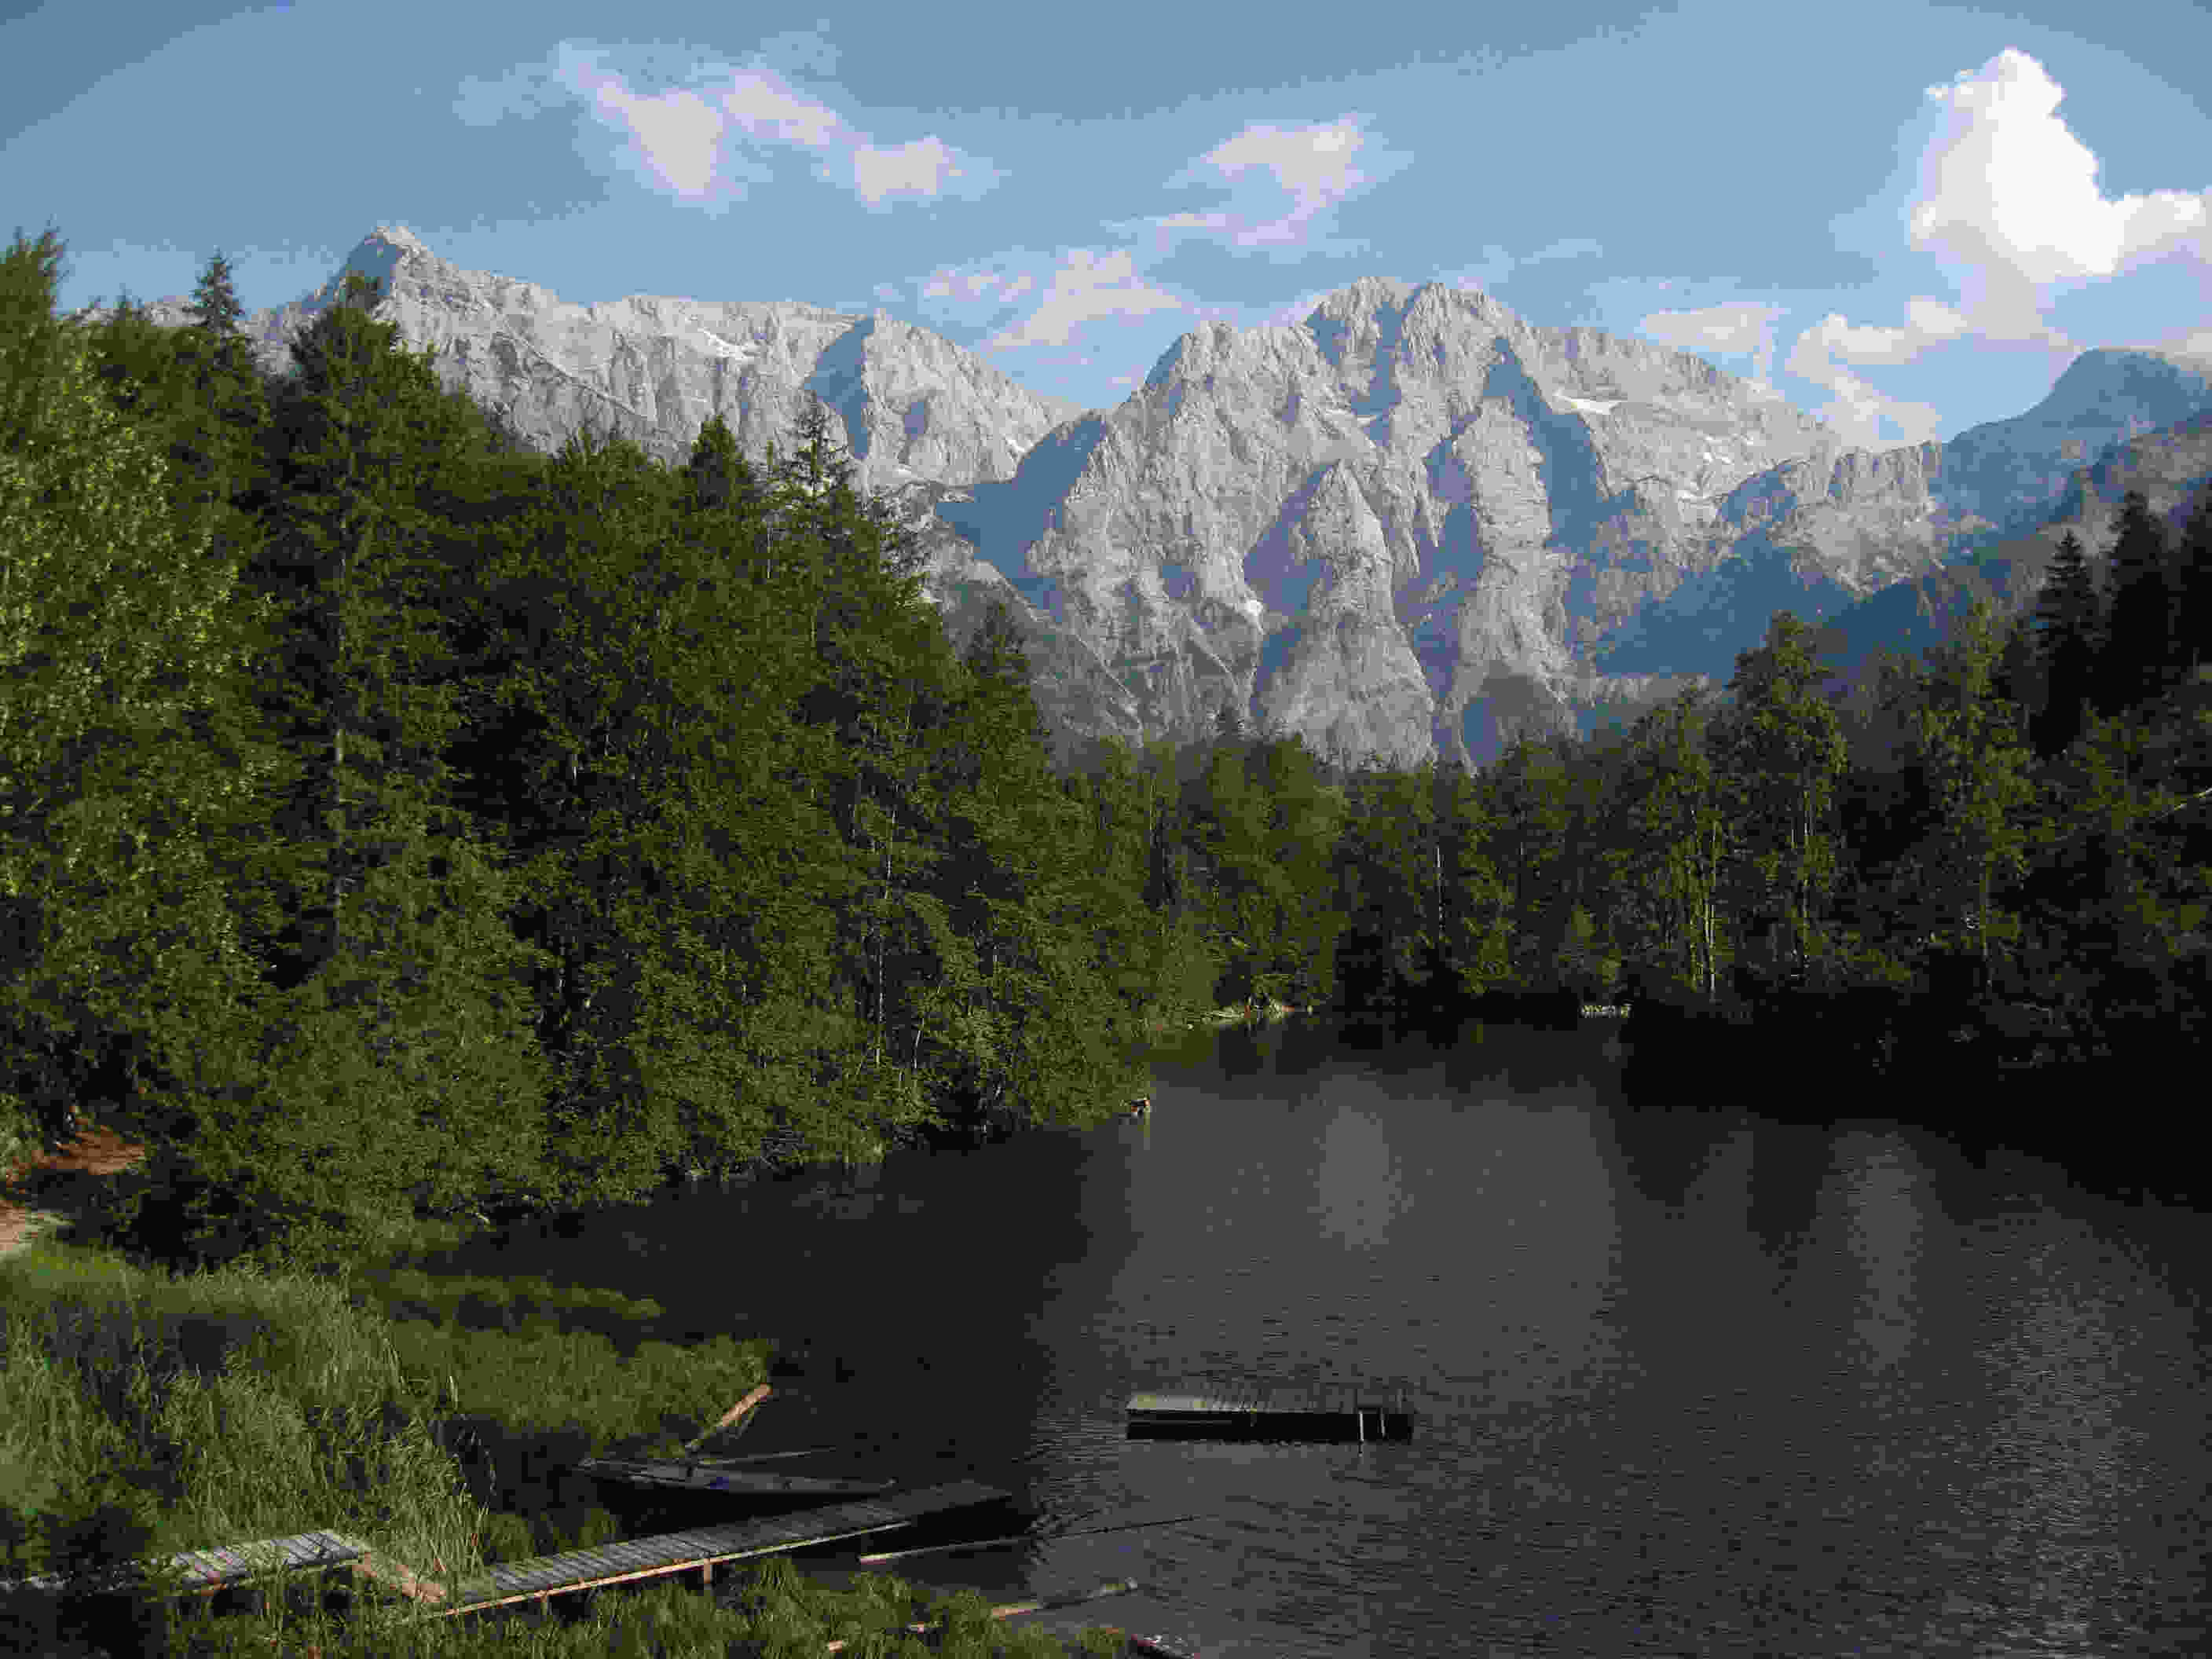
\includegraphics[width=7cm]{BergSee1.jpg}
	\caption{Snapshot taken at the beginning of a mountain hike.}
	\label{fig:image}
\end{figure}


We use the concept of datapoints in a highly abstract and 
therefore very flexible manner. datapoints can represent 
very different types of objects. For an image processing 
application it might be useful to define datapoints as images. 

A recommendation system might use datapoints to represent 
customers.  datapoints might represent time periods, animals, 
mountain hikes, proteins or humans. The meaning or definition 
of what datapoints represent is nothing but a design choice. 
 
One practical requirement for a useful definition of datapoints is 
that we should have access to many of them. ML methods typically 
rely on constructing estimates for quantities of interest by averaging 
over datapoints. These estimates are often more accurate the more 
datapoints are used for the averaging. 

A key parameter of a dataset is the number $\samplesize$ of individual 
datapoints it contains. The number of datapoints within a dataset is 
also referred to as the sample size. Statistically, the larger the sample size $\samplesize$ 
the better. However, there might be restrictions on computational 
resources that limit the maximum sample size $\samplesize$ that can be 
processed. 

Figure \ref{fig:two_main_parameters} illustrates two key 
parameters of a dataset. Beside the sample size $\samplesize$, a second 
key parameter of a dataset is the number of features used to characterize 
individual datapoints. 

\begin{figure}[htbp]
	\centering
	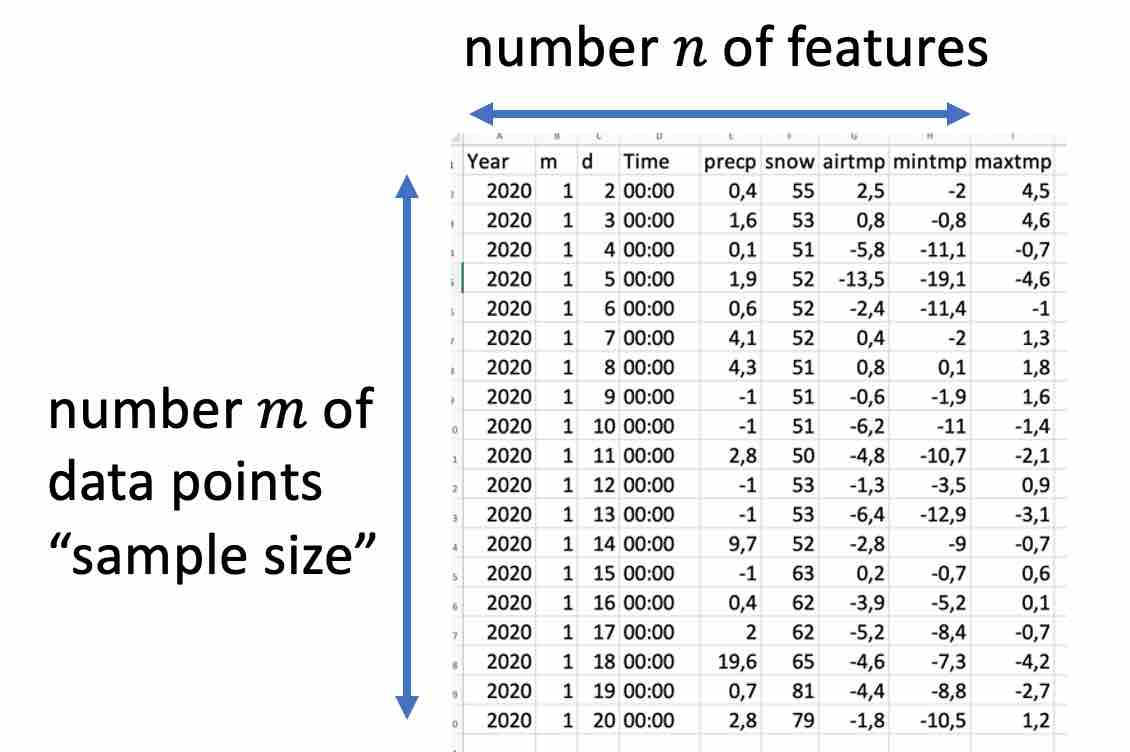
\includegraphics[width=7cm]{DataSet.jpg}
	\caption{Two main parameters of a dataset are the number 
		$\samplesize$ of datapoints it contains and the number 
		$\featuredim$ of features used to characterize individual 
		datapoints. A very important characteristic of a dataset 
		is the ratio $\samplesize/\featuredim$. }
	\label{fig:two_main_parameters}
\end{figure}


For most applications, it is impossible to have full access to 
every single microscopic property of a datapoint. Consider a 
datapoint that represents a vaccine. A full characterization of 
such a datapoint would require to specify its chemical composition 
down to level of molecules and atoms. Moreover, there are 
properties of a vaccine that depend on the patient who 
received the vaccine. 

It is useful to distinguish between two different groups of 
properties of a datapoint. The first group of properties is 
referred to as {\bf features}  and the second group of properties 
is referred to as {\bf label} (some authors refer to labels also 
as {\bf target} or {\bf output}). 

The distinction between features and labels is somewhat 
blurry. The same property of a datapoint might be used 
as a feature in one application, while it might be used as 
a label in another application. 

As an example, consider feature learning for datapoints 
representing images. One approach to learn representative 
features of an image is to use some of the image pixels as 
the label or target pixels. We can then learn new features 
by learning  a feature map that allows to predict the target 
pixels. 

\subsection{Features}
\label{sec_feature_space}
%The features of a datapoint are properties that can be computed, measured or 
%determined easily without requiring (significant) repetitive human labour. Determining 
%features of a datapoint typ be automated and performed efficiently. 

Similar to the definition of datapoints, also the choice of which 
properties to be used as features of a datapoint is a design choice. 
As a rule of thumb, features are properties or quantities that can be 
computed or measured easily. This is only an informal characterization 
since there is no widely-applicable measure for the difficulty in 
measuring a specific property. 

Modern information-technology, including smartphones or wearables, 
allows to measure a huge number of properties about datapoints in 
many application domains. Consider a datapoint representing the book 
author ``Alex Jung''. Alex uses a smartphone to take snapshots. 
Let us assume that Alex takes five snapshots per day on average (sometimes 
more, e.g., during a mountain hike). 

We conclude that Alex takes more than $1000$ snapshots per year. 
Each snapshot contains around $10^{6}$ pixels. Let us use each  
greyscale level of an individual pixel in those snapshots as features. 
This results in more than $10^{9}$ features (per year!). If we stack all 
those features into a single feature vector $\vx$, its length $\featurelen$ 
would be of the order of $10^{9}$. 

Many important ML applications involve datapoints represented by very 
long feature vectors. To process such high-dimensional data, modern 
ML methods rely on concepts from high-dimensional statistics \cite{BuhlGeerBook,Wain2019}. 
One such concept from high-dimensional statistics is the notion 
of sparsity. Sparsity based methods, which we discuss in Section \ref{sec_lasso}, 
exploits the tendency of high-dimensional datapoints to be aligned along 
some low-dimensional subspace.  

%If we develop a ML method that can use snapshots taken by a digital 
%camera, then these snapshots might be a useful choice for the features. 
%However, if we only have a thermometer at our disposal then we might 
%only use the measured temperature as the feature. In what follows we 
%will denote the total number of features used to describe a datapoint 
%by the letter $\featurelen$. 


%For a datapoint represented by a snapshot (see Figure \ref{fig:image}), we could use the red, green and blue intensities of 
%all image pixels as features. However, we could also use only the averages (over all pixels) of red, green and blue intensity. 
At first sight it might seem that ``the more features the better'' 
since using more features might convey more relevant information 
to achieve the overall goal. However, as we discuss in Chapter \ref{ch_overfitting_regularization}, 
it can actually be detrimental to the performance of ML methods 
to use an excessive amount of (irrelevant) features. 

Using too many irrelevant features might overwhelm or jam ML 
algorithms, which should invest their computational resources 
mainly in the processing of the most relevant features. It is difficult 
to give a precise characterization on the maximum number of 
features that should be used to characterize the datapoints 
arising in a given application. As a rule of thumb, the number $\samplesize$ 
of (labeled) datapoints provided to a ML method should be 
much larger than the number $\featurelen$ of numeric features.

The informal condition $\samplesize/\featurelen \gg 1$ can be ensured 
by either collecting a sufficiently large number $\samplesize$ of datapoints 
or by using a sufficiently small number $\featurelen$ of features. In what 
follows, we discuss how each of these two complementary approaches 
can be implemented. 

The acquisition of (labeled) datapoints might be costly, requiring human 
experts labour. Instead of collecting more raw data, it might 
be possible to generate synthetic data. Section \ref{sec_data_augmentation} 
discusses how intrinsic symmetries of datasets can be used to augment 
the raw data with synthetic data. 

As an example for an intrinsic symmetry of data, consider datapoints 
representing an image. We assign each image the label $y=1$ if it shows 
a cat and $y=-1$ otherwise. For each image with known label we can 
generate several other images with the same label. This other images 
are simply obtained by image transformation such as rotations or 
re-scaling (zoom-in or zoom-out) that do not change the depicted 
objects. We will see in Chapter \ref{ch_overfitting_regularization} 
that regularization techniques can be interpreted as an implicit 
data augmentation.  

Instead of collecting more datapoints to ensure the condition $\samplesize/\featurelen$, 
we can use try to reduce the number $\featurelen$ of features used to 
characterize datapoints. In some applications, we might use some domain 
knowledge to choose the most relevant features. For other applications, 
it might be difficult to tell which quantities are the best choice for features. 
Chapter \ref{ch_FeatureLearning} will discuss some data-driven methods 
for extracting a small number of relevant features of datapoints. 
%Choosing ``good'' features of the datapoints arising within a given ML application 
%is far from trivial and might be the most difficult task within the overall ML application. 
%The family of ML methods known as {\bf kernel methods} \cite{LampertNowKernel} 
%is based on constructing efficient features by applying high-dimensional {\bf feature maps}. 

%Instead of explicitly learning a small set of relevant features, {\bf deep learning methods} 
%(see Section \ref{sec_deep_learning}), 
%(``tuning'') \cite{Goodfellow-et-al-2016}. We will discuss the very basic ideas behind 
%such {\bf feature learning} methods in Chapter \ref{ch_FeatureLearning} but for now 
%assume the task of selecting good features is already solved. 

A datapoint is typically characterized by several individual features 
$x_{1},\ldots,x_{\featuredim}$. It is convenient to stack the individual 
features into a single feature vector 
\begin{equation}
\nonumber 
\vx=\big(x_{1},\ldots,x_{\featuredim}\big)^{T} \in \mathbb{R}^{\featuredim}. 
\end{equation}
Each datapoint is then characterized by such a feature vector $\vx$. 
The feature vectors of datapoints take on values out of some {\bf feature space}, 
which we denote as $\featurespace$. 

The feature space is a design choice as it depends on what properties of a 
datapoint we use as its features. This design choice should take into account 
the statistical properties of the data as well as the available computational infrastructure. 
If the computational infrastructure allows for efficient numerical linear algebra, 
then using $\featurespace = \mathbb{R}^{\featurelen}$ might be a good choice.
For a computational infrastructure that allows to efficiently process networks 
or graphs, we could use the nodes of a graph as the feature space (see Section \ref{sec_network_lasso}). 

%In general, to obtain computationally efficient ML methods one typically uses 
%feature spaces $\featurespace$ with a rich mathematical structure.

%Another choice for the feature space is discussed in Section \ref{}. 
%This can be useful for {\bf network-structured datasets} where the datapoints can be 
%compared with each other by some application-specific notion of similarity %\cite{WhenIsNLASSO,NNSPFrontiers2018,LogisticNLasso,JungTVMin2019}. 
%These approaches use as a feature space the node set of an ``empirical graph'' 
%whose nodes represent individual datapoints. The edges in the empirical graph 
%encode similarities between individual datapoints. 
 
The Euclidean space $\mathbb{R}^{\featuredim}$ is an example 
of a feature space with a rich geometric and algebraic structure \cite{RudinBookPrinciplesMatheAnalysis}. 
The algebraic structure of $\mathbb{R}^{\featuredim}$ is defined 
by vector addition and multiplication of vectors with scalars. 

The geometric structure of $\mathbb{R}^{\featuredim}$ is obtained 
by the Euclidean norm as a measure for the distance between two 
elements of $\mathbb{R}^{\featuredim}$. 

The algebraic and geometric structure of  $\mathbb{R}^{\featuredim}$ 
often enables an efficient search over $\mathbb{R}^{\featuredim}$ to 
find elements with desired properties. Chapter \ref{sec_ERM_lin_reg} 
discusses examples of such search problems in the context of learning 
an optimal hypothesis. 

Beside the computational infrastructure, also the statistical properties 
of the data should be taken into account for the choice of feature space. 
The linear algebraic structure of $\mathbb{R}^{\featuredim}$ allows to 
efficiently represent and approximate datasets that are well aligned 
along linear subspaces. Section \ref{sec_pca} discusses methods that learn 
such approximations. The geometric structure of $\mathbb{R}^{\featuredim}$ 
is used in Chapter \ref{ch_Clustering} to organize data sets into few coherent groups 
or cluster. 

Throughout this book we will mainly use the feature space $\mathbb{R}^{\featuredim}$ 
with dimension $\featuredim$ being the number of features of a datapoint. This 
feature space has proven useful in many ML applications due to availability 
of efficient soft- and hardware for numerical linear algebra. Moreover, the 
algebraic and geometric structure of $\mathbb{R}^{\featuredim}$ seems to 
reflect the intrinsic structure of the data generated in many important 
application domains.\footnote{This should not be too surprising as the 
Euclidean space has evolved as a mathematical abstraction of physical phenomena.}

%Using RGB intensities (modelled as real numbers) of the pixels within a (rather small) $512 \times 512$ pixel bitmap, 


Consider datapoints representing images with $512$ by $512$ pixels. 
A natural construction for the feature vector of such datapoints is to 
stack the red, green and blue intensities for all image pixels (see Figure \ref{fig_snapshot_pixels}). 
We end up with a feature vectors belonging to the feature space 
$\featurespace=\mathbb{R}^{\featuredim}$ of (rather large) dimension 
$\featuredim = 3 \cdot 512^2$. Indeed, for each of the $512 \times 512$ 
pixels we obtain $3$ numbers which encode the red, green and blue colour 
intensity of the respective pixel (see Figure \ref{fig_snapshot_pixels}). 

In some applications, it is less obvious how to represent datapoints 
by a numeric feature vector in $\mathbb{R}^{\featurelen}$. The subfield 
of feature learning studies methods that map non-numeric data to numeric 
feature vectors in $\mathbb{R}^{\featuredim}$. These methods aim to 
structures in datasets that resemble the algebraic and geometric structure 
of $\mathbb{R}^{\featurelen}$. A quite impressive example for such methods 
have been developed for textual data \cite{Mikolov2013}. 



\begin{figure}[htbp]
	\begin{center}
		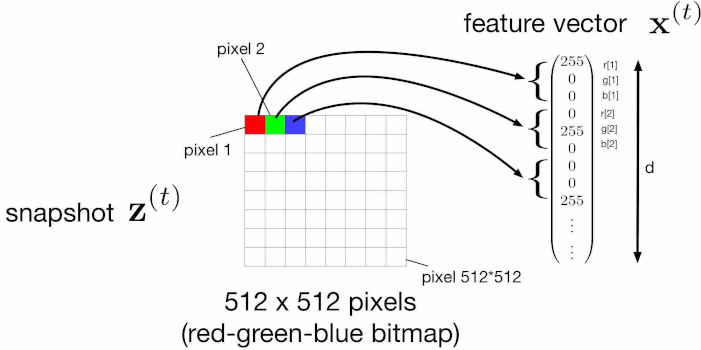
\includegraphics[width=8cm]{RumbaSnapshotFeature1.jpg}  
	\end{center}
	\caption{If the snapshot $\vz^{(\sampleidx)}$ is stored as a $512 \times 512$ RGB bitmap, we could use as 
		features $\vx^{(\sampleidx)} \in \mathbb{R}^{\featuredim}$ the red-, green- and blue component of each pixel 
		in the snapshot. The length of the feature vector would then be $\featuredim= 3 \cdot 512 \cdot 512 \approx 786000$. }
	\label{fig_snapshot_pixels}
	% \caption{A Simple Classification Example}\label{fig:A Simple Classification Example}
\end{figure}

%Our goal is to infer the current location $\state_{\timeidx}= \gridcell{x_{\timeidx}}{y_{\timeidx}}$ of \rumba\, 
%at time $\timeidx$ based only on the snapshot $\vz^{(\timeidx)}$ which is represented by the feature vector $\vx^{(\timeidx)}$. 
\subsection{Labels}
\label{sec_labels}

Besides the features of a datapoint, there are other properties of a datapoint that represent 
some higher-level information or ``quantity of interest'' 
associated with the datapoint. We refer to the higher level information, or quantity of 
interest, associated with a datapoint as its \emph{label} (or ``output'' or ``target''). 
In contrast to features, determining the value of labels is more difficult to automate. 
Many ML methods revolve around finding efficient ways to determine the label of a 
datapoint given its features. 

As already mentioned above, the distinction of datapoint properties into 
labels and those that are features is blurry. Roughly speaking, labels are 
properties of datapoints that might only be determined with the help of 
human experts. For datapoints representing humans we could define 
its label $y$ as an indicator if the person has flu ($y=1$) or not ($y=0$). 
This label value can typically only be determined by a physician. However, 
in another application we might have enough resources to determine the 
flu status of any person of interest and could use it as a feature that 
characterizes a person. 

Consider a datapoint that represents some hike, at the 
start of which the snapshot in Figure \ref{fig:image} has
 been taken. The features of this datapoint could be the 
 red, green and blue (RGB) intensities of each pixel in the 
 snapshot in Figure \ref{fig:image}. We stack these RGB 
 values into a vector $\vx \in \mathbb{R}^{\featurelen}$ 
 whose length $\featurelen$ is three times the number 
 of pixels in the image. 
 
 The label $y$ associated with a datapoint (which represents 
 a hike) could be the expected hiking time to reach the mountain in the 
snapshot. Alternatively, we could define the label $y$ as 
the water temperature of the lake visible in the snapshot. 

The label space $\labelspace$ of an ML problem contains all 
possible label values of datapoints. We refer to ML problems involving 
the $\labelspace = \mathbb{R}$ as a {\bf regression problem}. 
It is also common to refer to ML problems involving a discrete 
(finite or countably infinite) label space as {\bf classification problems}. 

ML problems with only two different label values are referred to as 
{\bf binary classification problems}. Examples of classification 
problems are: detecting the presence of a tumour in a tissue, 
classifying persons according to their age group or detecting 
the current floor conditions ( ``grass'', ``tiles'' or ``soil'') for 
a mower robot. 

The distinction between regression and classification problems is 
somewhat blurry. Consider a binary classification problem based 
on datapoints whose label $y$ takes on values $-1$ or $1$. We 
could turn this into a regression problem by using a new label 
$y'$ which is defined as the confidence in the label $y$ being 
equal to $1$. Given $y'$ we can obtain $y$ by thresholding, 
$y=1$ if $y'\geq0$ whereas $y=-1$ if $y' <0$. 


A datapoint is called \emph{labeled} if, besides its features $\vx$, 
the value of its label $y$ is known.The acquisition of labeled data 
points typically involves human labour, such as handling a water 
thermometer at certain locations in a lake. In other applications, 
acquiring labels might require sending out a team of marine biologists 
to the Baltic sea \cite{MLMarineBiology}, running a particle physics 
experiment at the European organization for nuclear research (CERN) \cite{MLCERN}, 
running animal testing in pharmacology \cite{MLPharma}. 

There are also online market places for human labelling 
workforce \cite{Mort2018}. In these market places, one 
can upload datapoints, such as images, and then pay 
some money to humans that label the datapoints, such 
as marking images that show a cat. 

Many applications involve datapoints whose features can be 
determined easily, but whose labels are known for few datapoints 
only. Labeled data is a scarce resource. Some of the most successful 
ML methods have been devised in application domains where 
label information can be acquired easily \cite{UnreasonableData}. 
ML methods for  speech recognition and machine translation can 
make use of massive labeled datasets that are freely available \cite{Koehn2005}. 

In the extreme case, we do not know the label of any single 
datapoint. Even in the absence of any labeled data, ML methods 
can be useful for extracting relevant information from 
features only. We refer to ML methods which do not require 
any labeled datapoints as {\bf unsupervised ML methods}. 
We discuss some of the most important unsupervised ML 
methods in Chapter \ref{ch_Clustering} and Chapter \ref{ch_FeatureLearning}).  

As discussed next, many ML methods aim at constructing 
(or finding) a ``good'' predictor $h: \featurespace \rightarrow \labelspace$ 
which takes the features $\vx \in \featurespace$ of a datapoint 
as its input and outputs a predicted label (or output, or target) 
$\hat{y} = h(\vx) \in \labelspace$. A good predictor should be 
such that $\hat{y} \approx y$, i.e., the predicted label $\hat{y}$ 
is close (with small error $\hat{y} - y$) to the true underlying label $y$. 

\subsection{Scatterplot} 
\label{equ_subsection_scatterplot}

Consider datapoints characterized by a single numeric feature $x$ 
and label $y$. 
%Each datapoint represents a particular day whose 
%feature and label are the minimum and maximum daytime temperature, 
%respectively, at some place in Finland. 
%We can obtain these datapoints via the weather recordings of 
%the Finnish Meteorological Institute (FMI). 
To gain more insight into the relation between the features 
and label of a datapoint, it can be instructive to generate a 
scatter plot as shown in Figure \ref{fig_scatterplot_temp_FMI}. 
A scatter plot depicts the datapoints $\vz^{(\sampleidx)}=(x^{(\sampleidx)},y^{(\sampleidx)})$ 
in a two-dimensional plane with the axes representing the values 
of feature $x$ and label $y$. 

A visual inspection of a scatterplot might suggest potential 
relationships between feature $x$ and label $y$. From Figure 
\ref{fig_scatterplot_temp_FMI}, it seems that there might be 
a relation between feature $x$ and label $y$ since datapoints 
with larger $x$ tend to have larger $y$. This makes sense since 
having a larger minimum daytime temperature typically implies 
also a larger maximum daytime temperature. 

We can obtain scatter plots for datapoints with more than two 
features using feature learning methods (see Chapter \ref{ch_FeatureLearning}). 
These methods transform high-dimensional datapoints, 
having billions of raw features, to three or two new features. 
These new features can then be used as the coordinates of 
the datapoints in a scatter plot.

%\begin{figure}[htbp]
%\begin{center}
%\begin{tikzpicture}
%    \begin{axis}[
%            axis x line=middle,
%            axis y line=middle,
%            enlarge y limits=true,
%            width=15cm, height=8cm,     % size of the image
%            grid = major,
%            grid style={dashed, gray!30},
%            ylabel=Ethereum closing price $y$,
%            xlabel=Bitcoin closing price $x$,
%         ]        
%          \addplot[only marks] table [x=CloseBTC, y=CloseETH, col sep = comma] {BTCETH-USD.csv};
%    \end{axis}
%\end{tikzpicture}
%\end{center}
%\caption{A scatter plot of some datapoints $(x^{(\sampleidx)},y^{(\sampleidx)})$ with Bitcoin 
%	closing price $x^{(\sampleidx)}$ and Ethereum closing price $y^{(\sampleidx)}$ at the 
%	$\sampleidx$-th day. Each datapoint $(x^{(\sampleidx)},y^{(\sampleidx)})$ is depicted by a 
%	dot located at the point with coordinates $x^{(\sampleidx)}$ and $y^{(\sampleidx)}$.\label{fig_scatterplot}} 
%\end{figure}

%\subsection{Missing Data} 
%The city of Turku is collecting information about pedestrian traffic by counting the number of pedestrians 
%passing by certain points in the city center. In Figure \ref{} we depict the recordings obtained from 
%few counting points over time. The recordings have some missing field which correspond to time steps 
%when for some reason the counting device did not deliver the count (estimate).  

\subsection{Probabilistic Models for Data} 
%Consider datapoints representing previous days in Finland. Each datapoint is 
%characterized by its (average) daytime temperature $x \in \mathbb{R}$. Assume we 
%have downloaded $\samplesize$ datapoints $\big(x^{(1)},\ldots,x^{(\samplesize)} \big)$. 
In what follows, we consider datapoints that are characterized by a 
single feature $x$. Many successful ML methods are based on a simple 
but crucial idea: Interpret datapoints as realizations of random variables. 
One of the most basic examples of a probabilistic model for the 
datapoints in ML is the {\bf ``independent and identically distributed'' (i.i.d.)} 
assumption. This assumption interprets datapoints $x^{(1)},\ldots,x^{(\samplesize)}$ 
as statistically independent realizations of one single random variable $x$.

It might seem somewhat awkward to interpret datapoints as realizations 
of random variables with some probability distribution $p(x)$. However, this 
interpretation allows us to use the properties of the probability distribution  
to characterize the statistical properties of collections of datapoints. 

The probability distribution $p(x)$ is either assumed to be 
known or estimated from data. It is often enough to estimate 
only some parameters of the distribution $p(x)$ such as the 
mean and the variance. Section \ref{sec_max_iikelihood}) 
discusses one particular approach to estimating the parameters 
of a probability distribution from datapoints. 


Some of the most basic and widely used parameters of a probability 
distribution $p(x)$ are the expected value or mean 
$$\mu_{x} = \expect\{x\} \defeq \int_{x} x p(x) dx$$ 
and the variance 
$$\sigma_{x}^{2} \defeq \expect\big\{\big(x-\expect\{x\}\big)^{2}\big\}.$$ 
These parameters can be estimated using the sample mean 
(average) and sample variance, 
\begin{equation} 
\label{equ_sample_mean_var}
\hat{\mu}_{x} \defeq (1/\samplesize) \sum_{\sampleidx=1}^{\samplesize} x^{(\sampleidx)}\mbox{ , and } \widehat{\sigma^{2}_{x}} \defeq (1/\samplesize) \sum_{\sampleidx=1}^{\samplesize} \big( x^{(\sampleidx)} - \hat{\mu}_{x} \big)^{2}.  
\end{equation} 
The sample mean and variance \eqref{equ_sample_mean_var} 
can be shown to be maximum likelihood estimators of the mean 
and variance of a normal (Gaussian) distribution $p(x)$ (see \cite[Chapter 2.3.4]{BishopBook}. 
%A widely used estimator for the square root of the variance is the 
%(sample) standard deviation $\hat{s}_{x} \defeq  \sqrt{(1/\samplesize-1) \sum_{\sampleidx=1}^{\samplesize} \big( x^{(\sampleidx)} - \hat{\mu}_{x} \big)^{2}}$. Using the feactor 




\section{The Model}
\label{sec_hypo_space}

%Consider the problem of classifying hand-drawings into two categories. 
%The first category consists of all hand-drawings that show an apple. 
%The second category consists of all hand-drawings that do not show 
%an apple. We consider each hand-drawing as one particular datapoint. 
%
%Each datapoint is associated with a numeric label $y \in \mathbb{R}$ 
%which is a percentage measuring how much the underlying hand-drawing 
%resembles an apple. Beside its label $y$, each datapoint (hand-drawing) 
%is characterized by a feature vector $\vx=\big(x_{1},\ldots,x_{n}\big)^{T}$ 
%obtained by stacking the greyscale intensities of a $128 \times 128$ 
%pixel image of the hand-drawing.  

Consider a ML application generating datapoints, each characterized 
by features $\vx \in \featurespace$ and label $y \in \labelspace$. The goal 
of ML is to learn a map $h(\vx)$ such that 
%Given a set of $m$ labeled datapoints (the ``training data'')
%\begin{equation} 
%\label{eq_def_training_set}
%\dataset  = \big\{ (\vx^{(1)},y^{(1)}), \ldots, (\vx^{(\samplesize)},y^{(\samplesize)}) \}
%\end{equation}
%ML methods learn 
\begin{equation} 
\label{equ_approx_label_pred}
y \approx \underbrace{h(\vx)}_{\hat{y}} \mbox{ for any datapoint}. 
\end{equation}  
The informal goal \eqref{equ_approx_label_pred} needs to be made precise 
in two aspects. First, we need to quantify the approximation error \eqref{equ_approx_label_pred} 
incurred by a given hypothesis map $h$. Second, we need to make precise 
what we actually mean by requiring \eqref{equ_approx_label_pred} to hold 
for ``any datapoint''. We solve the first issue by the concept of a loss 
function in Section \ref{sec_lossfct}. The second issue is then solved 
in Chapter \ref{ch_Optimization} by using a simple probabilistic model 
for data. 

 %also those not contained in the training set \eqref{eq_def_training_set}. 

%????
%Consider the cleaning robot \rumba\, which is depicted in Figure \ref{fig:cleaning_robot}. 
%A routine task of \rumba\, is to determine (predict) the coordinate $y^{(\sampleidx)} \in \mathbb{R}$ 
%of its current location at time $\sampleidx$. The prediction must be based solely on the features 
%$\vx^{(\sampleidx)} \in \mathbb{R}^{\featuredim}$ of the snapshot $\vz^{(\sampleidx)}$ delivered 
%by the on-board camera at time $\sampleidx$. ?????

%To have any chance to solve this task, we must assume (or hypothesize) 
%an underlying relation between the features $\vx$ and the label $y$. 
%Each ML method uses such an assumption indirectly by restricting the set 
%of possible hypothesis maps $h$ to 
%
%We 
%represent this relation between features $\vx$ and label $y$ using a 
%{\bf hypothesis} $h: \featurespace \rightarrow \labelspace$. 
%A hypothesis is a map or function, which maps the feature vector 
%$\vx^{(\sampleidx)}$ of a datapoints to a predicted label $\hat{y} = h(\vx)$. 

The main goal of ML is to learn a good hypothesis $h$ from some training data. 
Given a good hypothesis map $h$, such that \eqref{equ_approx_label_pred} 
is satisfied, ML methods use it to predict the label of any datapoint. 
The prediction $\hat{y}=h(\vx)$ is obtained by evaluating the hypothesis 
for the features $\vx$ of a datapoint. We will use the term predictor map 
for the hypothesis map to highlight its use for computing predictions. 

If the label space $\labelspace$ is finite, such as $\labelspace=\{-1,1\}$, 
we refer to a hypothesis also as a {\bf classifier}. For a finite label space 
$\labelspace$ and feature space $\featurespace=\mathbb{R}^{\featuredim}$, 
we can characterize a particular classifier map $h$ using its {\bf decision boundary}. 
The decision boundary of a classifier $h$ is the set of boundary points 
between the different {\bf decision regions}
\begin{equation} 
\label{equ_decision_region}
\mathcal{R}_{a} \defeq \{ \vx: \hat{y}= a \} \subseteq \featurespace. 
\end{equation}% of the feature space $\featurespace$. 
Each label value $a \in \labelspace$ is associated with a decision 
region $\mathcal{R}_{a}$. For a given label value $a \in \labelspace$, 
the decision region $\mathcal{R}_{a}$ contains all feature vectors 
$\vx \in \featurespace$ which are mapped to this label value, $\hat{y}=a \in \labelspace$. 

%A reasonable hypothesis $h$ should approximate the true label $y^{(\sampleidx)}$ 
%as accurately as possible such that $\hat{y}^{(\sampleidx)}=h(\vx^{(\sampleidx)}) \approx y^{(\sampleidx)}$ 
%at every time $\sampleidx$. Note that computing the prediction $\hat{y}=h(\vx)$ amounts to the evaluation 
%of a map $h(\cdot)$ for the particular argument $\vx$ (see Figure \ref{fig_feature_map_eval}). This seems 
%trivial, but in many ML applications the feature $\vx$ and the predictor $h(\cdot)$ can be very complicated 
%(high-dimensional) objects. Using feature vectors with millions of entries is not an exception but rather the 
%rule (see Figure \ref{fig_snapshot_pixels}). Much of ML theory revolves around the analysis and design of 
%automated methods for finding good predictors $h$ which can be evaluated efficiently. 



\begin{figure}[htbp]
%\begin{minipage}{\textwidth}
%\begin{center}
%\begin{tikzpicture}[auto,bend angle=30]
%  \filldraw[fill=red!20,snake=bumps] (0,0) rectangle (6,4);
%  \node[] (A) at (3,2) {$\featurespace$};
%  \fill (5cm,3) circle (2pt)  node[above] (C) {$\vx \in \featurespace$};
%   
%      \draw [ultra thick] (12,2) circle (2cm);
%        \node[] (B) at (12,2) {$\labelspace$};
%         \fill  (11.5,2.5)  circle (2pt) node[above] (D) {$\hat{y} \in \labelspace$};    
%         \draw [->,thick,dashed] (5,3)   --  (11.5,2.5) node[above,midway] {$h(\vx)$} ;
%\end{tikzpicture}
%\end{center}
%\end{minipage}
\begin{minipage}{\textwidth}
\begin{center}
   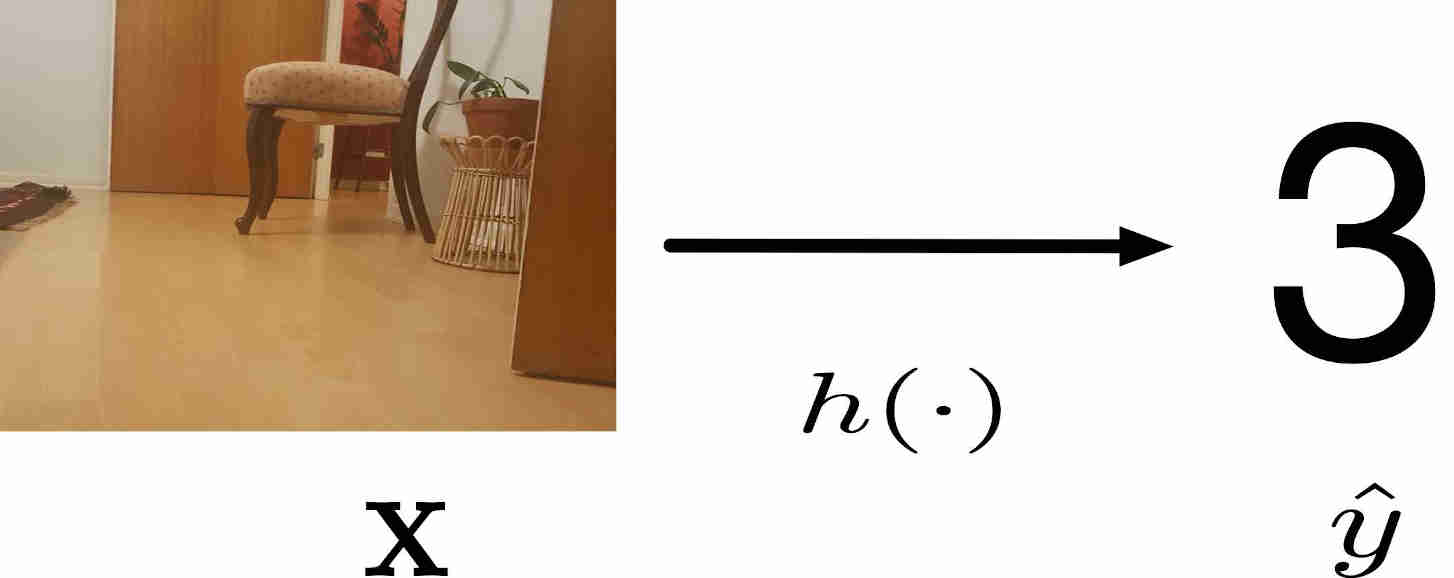
\includegraphics[width=0.7\textwidth]{HypoMap1.jpg}  
   \end{center}
\end{minipage}
\caption{A predictor (hypothesis) $h$ maps features $\vx\!\in\!\featurespace$, of 
	an on-board camera snapshot, to the prediction $\hat{y}\!=\!h(\vx)\!\in\!\labelspace$ 
	for the coordinate of the current location of a cleaning robot. ML methods use data 
	to learn predictors $h$ such that $\hat{y}\!\approx\!y$ (with true label $y$).}
\label{fig_feature_map_eval}
\end{figure}

In principle, ML methods could use any possible map $h: \featurespace \rightarrow \labelspace$ 
to predict the label $y \in \labelspace$ via computing $\hat{y} = h(\vx)$. 
However, any ML method has only {\bf limited computational resources} 
and therefore can only make use of a subset of all possible predictor maps. 
This subset of computationally feasible (``affordable'') predictor maps 
is referred to as the {\bf hypothesis space} or {\bf model} underlying 
a ML method. 

The largest possible hypothesis space $\hypospace$ is the set 
$\labelspace^{\featurespace}$ constituted by all maps from the 
feature space $\featurespace$ to the label space $\labelspace$.
The notation $\labelspace^{\featurespace}$ has to be understood 
a symbolic shorthand denoting the set of all maps from $\featurespace$ to $\labelspace$. 
The set $\labelspace^{\featurespace}$ does in general not behave like 
powers of numbers such as $4^5$. 


The hypothesis space $\hypospace = \labelspace^{\featurespace}$ 
is rarely used in practice since it is simply too large to work 
within a reasonable amount of computational resources.  
As depicted in Figure \ref{fig_hypo_space}, ML methods 
typically use a hypothesis space $\hypospace$ that is a tiny 
subset of $\labelspace^{\featurespace}$.  

The preference for a particular hypothesis space often depends 
on the available computational infrastructure available to a ML method. 
Different computational infrastructures favour different hypothesis 
spaces. ML methods implemented in a small embedded system, might 
prefer a linear hypothesis space which results in algorithms that require 
a small number of arithmetic operations. Deep learning methods 
implemented in a cloud computing environment typically use much larger 
hypothesis spaces obtained from deep neural networks. 

For the computational infrastructure provided by a {\bf spreadsheet software}, 
we might use a hypothesis space constituted by maps $h: \featurespace \rightarrow \labelspace$ 
which can be implemented easily by a spreadsheet (see Table \ref{table_lookup}). 
If we instead use the programming language Python to implement 
a ML method, we can obtain a hypothesis class by collecting all possible 
Python subroutines with one input (scalar feature $x$), one output 
argument (predicted label $\hat{y}$) and consisting of less than $100$ 
lines of code. %(see Figure \ref{fig_hypospace_Python}). 

If the computational infrastructure allows for efficient numerical 
linear algebra and the feature space is the Euclidean space $\mathbb{R}^{\featuredim}$, 
a popular choice of the hypothesis space is  
\begin{align}
\label{equ_def_hypo_linear_pred}
\hspace*{-3mm}\hypospace^{(\featuredim)} \!\defeq\!\{ h^{(\vw)}\!:\!\mathbb{R}^{\featuredim}\!\rightarrow\!\mathbb{R}\!:\!h^{(\vw)}(\vx)\!=\!\vx^{T} \vw \mbox{ with some weight vector } \vw\!\in\!\mathbb{R}^{\featuredim} \}.  
\end{align}

The hypothesis space \eqref{equ_def_hypo_linear_pred} is constituted 
by the linear maps (functions) $h^{(\vw)}: \mathbb{R}^{\featuredim} \rightarrow \mathbb{R}$. 
The function $h^{(\vw)}$ maps the feature vector $\vx \in \mathbb{R}^{\featuredim}$ 
to the predicted label (or output) $h^{(\vw)}(\vx) = \vx^{T} \vw \in \mathbb{R}$. 
For $\featuredim\!=\!1$ the feature vector reduces a single feature $x$ and 
the hypothesis space \eqref{equ_def_hypo_linear_pred} consists of all maps 
$h^{(w)}(x) = w x$ with some weight $w \in \mathbb{R}$ (see Figure \ref{scalar_lin_space}). 


\begin{figure}[htbp]
    \centering
    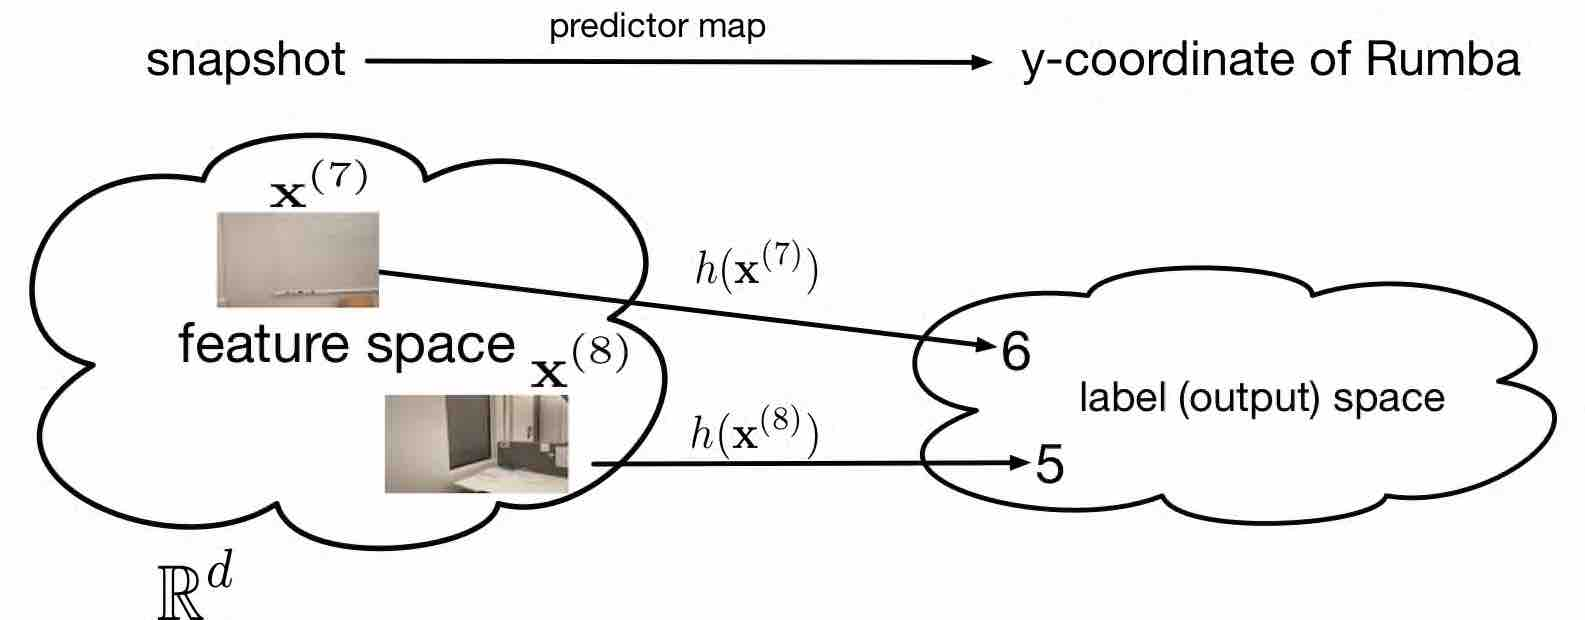
\includegraphics[width=0.7\textwidth]{HypothesisMapRumba.jpg}  
    \caption{A predictor (hypothesis) $h: \featurespace \rightarrow \labelspace$ takes 
    	the feature vector $\vx^{(\timeidx)} \in \featurespace$  (e.g., representing the 
    	snapshot taken by \rumba\, at time \timeidx) as input and outputs a predicted 
    	label $\hat{y}_{\timeidx}=h(\vx^{(\timeidx)} )$ (e.g., the predicted $y$-coordinate 
    	of \rumba\, at time $\timeidx$). A key problem studied within ML is how to 
    	automatically learn a good (accurate) predictor $h$ such that $y_{\timeidx} \approx h(\vx^{(\timeidx)} )$. }
%    \caption{Hypothesis Map}
\label{fig:Hypothesis Map}
\end{figure}

%\begin{figure}[htbp]
%    \centering
%    \includegraphics[natwidth=800,natheight=600,width=\textwidth]{HypoSpaceLinear.png}  
%    \caption{The hypothesis space $\hypospace$ which is constituted by all linear maps $h^{(w)}(x)=x w$ of the single feature $x$.}
%%    \caption{Hypothesis Map}\label{fig:Hypothesis Map}
%\label{scalar_lin_space}
%\end{figure}

\begin{figure}[htbp]
\begin{center}
    \begin{tikzpicture}
          \begin{axis}
     [ylabel=$h(x)$,scale=0.9,
              xlabel=$x$,%grid, 
              axis x line=center,
  axis y line=center,
  xtick={1},
  ytick={1},
  xlabel={feature $x$},
  ylabel={$h^{(w)}(x)$},
  xlabel style={right},
  ylabel style={above},
  xmin=-1.4,
  xmax=3.5,
  ymin=-1.1,
  ymax=1.1
  ]
  \addplot [smooth, color=red, ultra thick] table [x=a, y=b, col sep=comma] {linear.csv} node [right,color=red] {$h^{(1)}(x)\!=\!x$};
  \addplot [color=blue, ultra thick] table [x=a, y=c, col sep=comma] {linear.csv} node [right,color=blue] {$h^{(0.2)}(x)\!=\!0.2x$}; 
  \addplot [color=black, ultra thick] table [x=a, y=d, col sep=comma] {linear.csv}node [right,color=black] {$h^{(0.7)}(x)\!=\!0.7x$}; 
 \end{axis}
%\node [right,color=red] at (8.3,1.5) {$h^{(\mathbf{w})} = 7(x^2 - x^3)$};
%\node [right,color=blue] at (2.7,0.5) {$h^{(\mathbf{w})} =x^2$};
%\node [right] at (3.5,2.2) {$h^{(\mathbf{w})}\!=\!x$};
     \end{tikzpicture}
     \vspace*{-4mm}
\end{center}
\caption{Three particular members of the hypothesis space 
	$\hypospace =\{ h^{(w)}: \mathbb{R} \rightarrow \mathbb{R}, h^{(w)}(x) = w \cdot x \}$ 
which consists of all linear functions of the scalar feature $x$. We can parametrize 
this hypothesis space conveniently using the weight $w\in \mathbb{R}$ as $h^{(w)}(x) = w \cdot x$.}
\label{scalar_lin_space}
\end{figure}

The elements of the hypothesis space $\hypospace$ in \eqref{equ_def_hypo_linear_pred} are  
parameterized by the weight vector $\vw \in \mathbb{R}^{\featuredim}$. 
Each map $h^{(\vw)} \in \hypospace$ is fully specified by the weight 
vector $\vw$. Instead of searching over the function space $\hypospace$ 
(its elements are functions!), we can equivalently search over all 
possible weight vectors $\vw \in \mathbb{R}^{\featuredim}$. 

The search space $\mathbb{R}^{\featuredim}$ is still (unaccountably) 
infinite but it has a rich geometric and algebraic structure that 
allows to efficiently search over this space. Chapter \ref{ch_GD} 
discusses methods that use the concept of gradients to implement  
an efficient search for good weights $\vw \in \mathbb{R}^{\featurelen}$. 

The hypothesis space \eqref{equ_def_hypo_linear_pred} is also appealing because 
of the broad availability of computing hardware such as graphic processing units. 
Another factor boosting the widespread use of \eqref{equ_def_hypo_linear_pred} 
might be the offer for optimized software libraries for numerical linear algebra. 

The hypothesis space \eqref{equ_def_hypo_linear_pred} can also be 
used for classification problems, e.g., with label space $\labelspace = \{-1,1\}$. 
Indeed, given a linear predictor map $h^{(\vw)}$ we can classify data 
points according to $\hat{y}\!=\!1$ for $h^{(\vw)}(\vx) \geq 0$ and $\hat{y}\!=\!-1$ 
otherwise. The resulting classifier is an example of a {\bf linear classifier}. 

The defining property of a linear classifier, which maps data points with features 
$\vx$ to a predicted label $\hat{y}$, is that its decision regions \eqref{equ_decision_region} 
are half-spaces. As illustrated in Figure \ref{fig_lin_dec_boundary}, the decision boundary of a linear classifier 
is a hyperplane $\{ \vx: \vw^{T} \vx = b \}$.

ML methods that use linear classifiers include logistic regression 
(see Section \ref{sec_LogReg}), the SVM (see Section \ref{sec_SVM}) and naive 
Bayes' classifiers (see Section \ref{sec_NaiveBayes}).
\begin{figure} 
	\begin{center}
		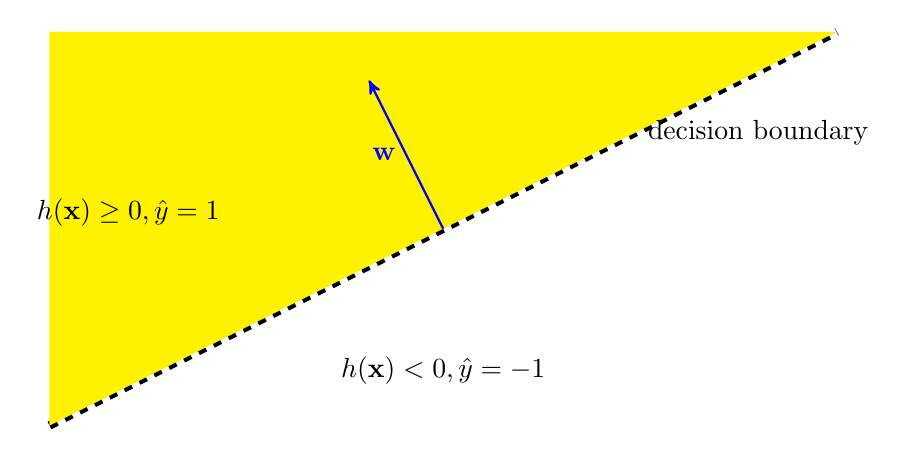
\begin{tikzpicture}[allow upside down, scale=1]
		\draw[dashed,line width=3pt] (0,0) -- (10,5)  [smooth, tension=0.5]
		node[sloped,inner sep=0cm,above,pos=.5,
		anchor=south west,
		minimum height=2cm,minimum width=1cm](N){adf};
		\path [fill=yellow] (0,0) -- (0,5) -- (10,5) -- (0,0); %to %[out=-80, in=160]
		\node [below] at (5,1) {$h(\vx)<0, \hat{y} = -1$};
		\node [below] at (9,4) {decision boundary};
		\node [below] at (1,3) {$h(\vx)\geq0, \hat{y} = 1$};
		\path (N.south west)
		edge[->,blue,thick] node[left] {$\mathbf{w}$} (N.north west);
		\end{tikzpicture}
	\end{center}
	\caption{A hypothesis $h: \featurespace\!\rightarrow\!\labelspace$ for a binary 
		classification problem, with label space $\labelspace=\{ -1,1\}$ and feature 
		space $\featurespace=\mathbb{R}^{2}$, can be represented conveniently via the 
		decision boundary (dashed line) which separates all feature vectors $\vx$ with 
		$h(\vx) \geq 0 $ from the region of feature vectors with $h(\vx)<0$. If the decision 
		boundary is a hyperplane $\{ \vx: \vw^{T} \vx = b \}$ (with normal vector 
		$\vw \in \mathbb{R}^{\featuredim}$), we refer to the map $h$ as a {\bf linear classifier}. }
	\label{fig_lin_dec_boundary}
\end{figure}

Despite all the above mentioned benefits of the hypothesis space \eqref{equ_def_hypo_linear_pred} 
it might seem too restrictive to consider only hypotheses that are linear functions 
of the features. Indeed, in most applications the relation between features $\vx$ 
and label $y$ of a datapoint is highly non-linear. We can then upgrade the 
linear hypothesis space by replacing the original features $\vx$ of a data 
point with some new features $\vz = {\bf \Phi} (\vx)$. The new features $\vz$ 
are obtained by applying some feature map $\phi$. If we apply a  
linear hypothesis to the new features $\vz$, we obtain a non-linear 
map from the original features $\vx$ to the predicted label $\hat{y}$, 
\begin{equation}
\label{equ_conc_featuremap_linear}
\hat{y} = \vw^{T} \vz = \vw^{T} {\bf \Phi} (\vx). 
\end{equation} 
Section \ref{sec_kernel_methods} discusses the family of 
kernel methods which are based on the concatenation \eqref{equ_conc_featuremap_linear} of 
(high-dimensional) feature maps ${\bf \Phi}(\cdot)$ 
with a linear hypothesis map. 


%Consider datapoints being images of animals with features $\vx$ 
%being the RGB values of pixels and the label $y$ being the confidence (on a scale $0,\ldots,100$) 
%that the image shows a cat. The relation between features and label is typically 
%a highly non-linear function. 

The hypothesis space \eqref{equ_def_hypo_linear_pred} can 
only be used for datapoints whose features are numeric 
vectors $\vx = (x_{1},\ldots,x_{\featuredim})^{T} \in \mathbb{R}^{\featuredim}$. 
In some application domains, such as natural language 
processing, there is no obvious natural choice for numeric 
features. However, since ML methods based on the hypothesis 
space \eqref{equ_def_hypo_linear_pred} are well developed 
(using numerical linear algebra), it might be useful to construct 
numerical features even for non-numeric data (such as text). 
For text data, there has been significant progress recently on 
methods that map a human-generated text into sequences of 
vectors (see \cite[Chap. 12]{Goodfellow-et-al-2016} for more details). 

%Since the choice of what features are used to characterize datapoints is a design choice, we can simply require the features 
%to be represented by vectors to allow the use of  
The hypothesis space $\hypospace$ used by a ML method is a {\bf design choice}. 
Some choices have proven useful for a wide range of applications (see Chapter \ref{ch_some_examples}). 
%As with the choice of what properties to use as features of a datapoint, 
In general, choosing a suitable hypothesis space requires a good 
understanding (``domain expertise'') of statistical properties of 
the data and the limitations of the available computational infrastructure. 

%One important aspect guiding the choice for the hypothesis space is the available 
%computational infrastructure. If we only have a spreadsheet program at our disposal 
%then it might be reasonable to use a hypothesis space which is constituted by maps 
%$h$ which can be represented by look-up tables (see Figure \ref{table_lookup}). 
%If our computational infrastructure allows for efficient numerical linear algebra. 
%which is the case for most desktop computers and scientific programming languages), 
%the linear hypothesis space \eqref{equ_def_hypo_linear_pred} might be useful.

%Note that the elements of the hypothesis space $\hypospace$ are maps $h$ from the feature space 
%to the label space of a given ML problem. 





%\begin{center}
%\framebox[0.96\textwidth]{
% \parbox{0.9\textwidth}{
%{\bf Exercise.} Given the hyperplane $\mathcal{C}=\{ \vx:  \vw^{T} \vx = 1 \}$ with vector $\vw = (1,0,0,1)^{T}$, can you find a 
%map $h: \mathbb{R}^{4} \rightarrow \mathbb{R}$ of the form $h(\vx) = \vu^{T} \vx +g$ with some vector $\vu \in \mathbb{R}^{4}$ and constant $g$, 
%such that $h(\vx)\geq 0$ for all $\vx$ above $\mathcal{C}$ and $h(\vx) < 0$ 
%for all $\vx$ below $\mathcal{C}$?
%}}
%\end{center}

%Consider the dataset depicted in Figure \ref{fig_scatterplot} consisting of historic information 
%about cryptocurrency prices. Each datapoint (depicted by a dot) corresponds to the cryptocurrency 
%statistics of one particular day. The $i$-th datapoint is characterized using the feature $x^{(\sampleidx)}$ 
%being the closing price of Bitcoin at day $\sampleidx$ and the label $y^{(\sampleidx)}$ being the closing 
%price of Ethereum at the same day. 
%
%If the relation $x \mapsto y$ cannot be well approximated by a linear function, we must 
%consider a hypothesis space which contains non-linear maps. In particular, we might 
%consider a hypothesis space which is constituted by polynomials, e.g., 
%$h(x) = w_{0} +w_{1} x + w_{2} x^2 + w_{3} x^{3}$, of a given maximum degree. 
%Figure \ref{fig_poly_hypo_space} depicts a particular predictor which belongs 
%to this larger hypothesis space. We will consider ML problems using a hypothesis 
%space of polynomial functions of a scalar feature in Section \ref{sec_polynomial_regression}. 
%
%\begin{figure}[htbp]
%\begin{center}
%    \begin{tikzpicture}
%          \begin{axis}
%     [ylabel=$h(x)$,
%     xscale=1,
%              xlabel=$x$,grid, 
%              axis x line=center,
%  axis y line=center,
%  xtick={-2,-1,...,2},
%  ytick={0,1,...,2},
%  xlabel={feature $x$},
%  ylabel={$h^{(\mathbf{w})}(x)$},
%  xlabel style={right},
%  ylabel style={above},
%  xmin=0,
%  xmax=1.2,
%  ymin=0,
%  ymax=1.1
%  ]
%
%  \addplot [smooth, color=red, ultra thick] table [x=a, y=b, col sep=comma] {polynomials.csv};    
%  \addplot [color=blue, ultra thick] table [x=a, y=c, col sep=comma] {polynomials.csv};     
%  \addplot [color=black, thick] table [x=a, y=d, col sep=comma] {polynomials.csv};      
% \end{axis}
%\node [right,color=red] at (5.5,1.5) {$h^{(\mathbf{w}_{1})}(x) = 7(x^2 - x^3)$};
%\node [right,color=blue] at (2.3,0.5) {$h^{(\mathbf{w}_{2})}(x) =x^2$};
%\node [right] at (2.5,2.8) {$h^{(\mathbf{w}_{3})}(x)\!=\!x$};
%     \end{tikzpicture}
%     \vspace*{-4mm}
%\end{center}
%\caption{Three particular members of the hypothesis space $\mathcal{H}_{\rm poly}^{(3)}$ 
%(see \eqref{equ_def_poly_hyposapce}) which consists of polynomials of degree at most $3$.}
%\label{fig_poly_hypo_space}
%\end{figure}


The design choice of the hypothesis space $\hypospace$ 
has to balance between two conflicting requirements.  
\begin{itemize} 
\item It has to be {\bf sufficiently large} such that it contains at least 
one accurate predictor map $\hat{h} \in \hypospace$. A hypothesis 
space $\hypospace$ that is too small might fail to include a predictor 
map required to reproduce the (potentially highly non-linear) relation 
between features and label. 

Consider the task of grouping or classifying images into 
``cat'' images and ``no cat image''. The classification of 
each image is based solely on the feature vector obtained 
from the pixel colour intensities. 

The relation between features and label ($y \in \{ \mbox{cat}, \mbox{no cat} \}$) 
is highly non-linear. Any ML method that uses a hypothesis space 
consisting only of linear maps will most likely fail to 
learn a good predictor (classifier). We say that a ML 
method {\bf underfits} the data if it uses a too small 
hypothesis space. 
\item It has to be {\bf sufficiently small} such that its processing fits the 
available computational resources (memory, bandwidth, processing time). 
We must be able to efficiently search over the hypothesis space to find 
good predictors (see Section \ref{sec_lossfct} and Chapter \ref{ch_Optimization}). 
This requirement implies also that the maps $h(\vx)$ contained in $\hypospace$ 
can be evaluated (computed) efficiently \cite{Austin2018}. Another important 
reason for using a hypothesis space $\hypospace$ not too large is to 
avoid {\bf overfitting} (see Chapter \ref{ch_overfitting_regularization}). 
If the hypothesis space $\hypospace$ is too large, then just by luck we 
might find a predictor which fits the training dataset well. Such a predictor 
might perform poorly on data which is different from the training data 
(it will not generalize well). 
\end{itemize}

The notion of a hypothesis space being too small or being 
too large can be made precise in different ways. The size of 
a finite hypothesis space $\hypospace$ can be defined as 
its cardinality $|\hypospace|$ which is simply the number of 
its elements. 

{\bf Example.} Consider datapoints represented by $100 \times 10\!=\!1000$ 
black-and-white pixels (see Figure \ref{fig_snapshot_pixels}) and 
characterized by a binary label $y \in \{0,1\}$. We can model such 
datapoints using the feature space $\featurespace = \{0,1\}^{1000}$ 
and label space $\labelspace = \{0,1\}$. The largest possible hypothesis 
space $\hypospace = \labelspace^\featurespace$ consists of all 
maps from $\featurespace$ to $\labelspace$. The size or cardinality 
of this space is $|\hypospace| = 2^{2^{1000}}$.

Many ML methods use a hypothesis space which contains 
infinitely many different predictor maps (see, e.g., \eqref{equ_def_hypo_linear_pred}). 
For an infinite hypothesis space, we cannot simply use the 
number of its elements as a measure for its size (since this number 
is not well-defined). Different concepts have been studied for 
measuring the size of infinite hypothesis spaces with the {\bf Vapnik–Chervonenkis (VC) dimension} 
being maybe the most famous one \cite{VapnikBook}. 

We will use a simplified variant of the VC dimension and define the 
{\bf effective dimension} of a hypothesis space $\hypospace$ 
as the maximum number $\sizehypospace$ of datapoints, drawn from 
a continues probability distribution, that can be perfectly fit (with probability one). 
For any set of $\sizehypospace$ datapoints with different features, we 
can always find a hypothesis $h \in \hypospace$ such that $y=h(\vx)$ 
for all datapoints $(\vx,y) \in \dataset$. 

Let us illustrate our concept for the size of a hypothesis space 
with two examples: linear regression and polynomial regression. 
Linear regression uses the hypothesis space 
$$\hypospace^{(\featuredim)} = \{ h: \mathbb{R}^{\featuredim} \rightarrow \mathbb{R}: h(\vx) = \vw^{T} \vx \mbox{ with some vector } \vw \in \mathbb{R}^{\featurelen}\}.$$ 
Consider a dataset $\dataset=\big( \big(\vx^{(1)} ,y^{(1)}\big),\ldots, \big(\vx^{(\samplesize)} ,y^{(\samplesize)}\big) \big)$ consisting of $\samplesize$ datapoints. 
Each datapoint is characterized by a feature 
vector $\vx^{(\sampleidx)} \in \mathbb{R}^{\featuredim}$ and a numeric label 
$y^{(\sampleidx)} \in \mathbb{R}$. 

Let us assume that datapoints are realizations of i.i.d.\ continuous random 
variables with the same probability density function. 
Under this assumption, the matrix 
$$\mathbf{X} = \big(\vx^{(1)},\ldots,\vx^{(\samplesize)}\big) \in \mathbb{R}^{\featuredim\times \samplesize},$$ 
which is obtained by stacking (column-wise) the feature vectors $\vx^{(\sampleidx)}$ (for $\sampleidx=1,\ldots,\samplesize$), 
is full rank with probability one. Basic linear algebra allows to show that 
the datapoints in $\dataset$ can be perfectly fit by a linear map $h \in \hypospace^{(\featuredim)}$ 
as long as $\samplesize \leq \featuredim$. In other words, for  $\samplesize \leq \featuredim$, we 
can find (with probability one) a weight vector $\hat{\vw}$ such that $y^{(\sampleidx)} = \hat{\vw}^{T} \vx^{(\sampleidx)}$ 
for all $\sampleidx=1,\ldots,\samplesize$. The effective dimension of the linear hypothesis space 
$\hypospace^{(\featuredim)}$ is therefore $\sizehypospace = \featuredim$. 

As a second example, consider the hypothesis space 
$\hypospace_{\rm poly}^{(\featuredim)}$ which is constituted 
by the set of polynomials with maximum degree $\featuredim$. 
The fundamental theorem of algebra tells us that any set 
of $\samplesize$ datapoints with different features can 
be perfectly fit by a polynomial of degree $\featuredim$ 
as long as $\featuredim \geq \samplesize$. Therefore, the 
effective dimension of the hypothesis space $\hypospace_{\rm poly}^{(\featuredim)}$ 
is $\sizehypospace=\featuredim$. Section \ref{sec_polynomial_regression} 
discusses polynomial regression in more detail. 


%For the sake of simplicity let us develop a simpler concept for the size of a hypothesis space. 
%Let us use the maximum number of arbitrary datapoints that can be perfectly fit using some 
%element of $\hypospace$ as the measure for the size of $\hypospace$. 

%???? remove?????
%The second aspect becomes relevant already for (seemingly) simple ML problems. Indeed, consider \rumba\, 
%which has to predict if it is moving towards a charging station at time $\sampleidx$, which is encoded by the 
%label $y^{(\sampleidx)} =-1$ or not, encoded by  $y^{(\sampleidx)} =1$. In order to determine if it is moving 
%towards a charging station, \rumba\, can only use the snapshot $\vz^{(\sampleidx)}$ generated by its on-board 
%camera at time $\sampleidx$. The snapshot is available as a black-white bitmap consisting of $512 \times 512$ 
%pixels. In order to construct a classifier, we represent the snapshot using a feature vector $\vx^{(\sampleidx)} \in \{0,1\}^{\featuredim}$ 
%of length $\featuredim =  512^2$ . 
%
%If we would use as hypothesis space $\hypospace_{\rm BW}$ the set of all possible maps from 
%the feature space $\featurespace= \{0,1\}^{512^{2}}$ (representing a BW bitmap) into the label 
%space $\labelspace=\{-1,1\}$, we would end up with a hypothesis space containing $2^{| \featurespace |} = 2^{2^{512^{2}}}$ 
%elements. Thus, the naive choice of a hypothesis space (which is to consider all possible 
%maps from feature to label space) for this (quite small) ML problem would already result 
%in a hypothesis space $\hypospace_{\rm BW}$
%
%??????

\begin{figure}[htbp]
\begin{center}
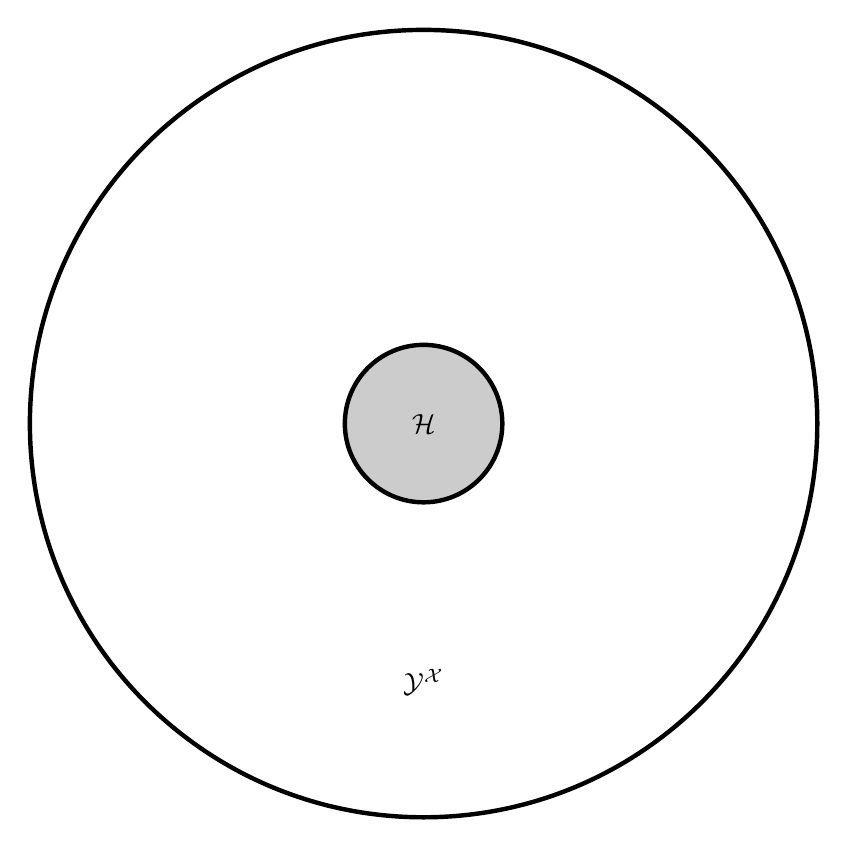
\begin{tikzpicture}[allow upside down, scale=1]
%(0,0)(0.70,1.9)(1.41,3.6)
%\draw plot [smooth, tension=0.5] coordinates{(2.13,5.1)(2.86,6.4)(3.62,7.5)(4.42,8.4)(5.30,9.1)(6.34,9.6)(7.13,9.8)(8.42,9.9)}
%\draw[red,line width=1pt] (0,0) -- (10,5)  [smooth, tension=0.5]
%node[sloped,inner sep=0cm,above,pos=.5,
%anchor=south west,
%minimum height=2cm,minimum width=1cm](N){};
%\path [fill=yellow] (0,0) -- (0,5) -- (10,5) -- (0,0); %to %[out=-80, in=160]
\node [below] at (5,-3) {$\labelspace^{\featurespace}$};
\draw [ultra thick] (5,0) circle (5cm);
\draw [ultra thick,fill=black!20] (5,0) circle (1cm);
\node [] at (5,0) {$\hypospace$};
%\path (N.south west)
%edge[->,blue,thick] node[left] {$\mathbf{w}$} (N.north west);
\end{tikzpicture}
\end{center}
\caption{The hypothesis space $\hypospace$ is a (typically very small) subset of the (typically very large) 
	set $\labelspace^{\featurespace}$ of all possible maps from feature space $\featurespace$ into the label 
	space $\labelspace$.}
\label{fig_hypo_space}
\end{figure}


\vspace*{2mm}
\begin{table}
\begin{center}
\begin{tabular}{ |c|c| }
  \multicolumn{1}{c}{feature $x$}
  &  \multicolumn{1}{c}{prediction $h(x)$} \\
\cline{1-2}
 0 & 0 \\
 \cline{1-2}
 1/10 & 10 \\
 \cline{1-2}
 2/10 & 3 \\
 \cline{1-2}
 \vdots & \vdots \\
 \cline{1-2}
 1 & 22.3 \\
\cline{1-2}
\end{tabular}
\end{center}
\caption{A spreadsheet representing a hypothesis map $h$ 
	in the form of a look-up table. The value $h(x)$ is given
	by the entry in the second column of the row whose first 
	column entry is $x$.}
\label{table_lookup}
\end{table}
\vspace*{2mm}

%\begin{figure}[htbp]
%%\resizebox {\textwidth} {!} {
%%\scalebox{.4}{
%\begin{tikzpicture}[scale=1,sharp corners=2pt,inner sep=7pt,node distance=.8cm,every text node part/.style={align=center}]
%\draw [draw=black] (0,-5.5) rectangle (15,4);
%\node[draw,right=1cm, minimum height = 2cm, minimum width = 3cm] (state0)
%{\begin{lstlisting}
%def predictor_map1(x):
%    return x*x
%\end{lstlisting}};
%\node[draw,right=1cm,below=2cm of state0, minimum height = 2cm, minimum width = 3cm](state2)
%{\begin{lstlisting}
%def predictor_map2(x):
%    return 3*x*x*x
%\end{lstlisting}};
%\node[draw,right=2cm of state0, minimum height = 2cm, minimum width = 3cm](state1)
%{\begin{lstlisting}
%def predictor_map3(x):
%    return 5*x
%\end{lstlisting}};
%\node[draw,below=2cm of state1, minimum height = 2cm, minimum width = 3cm](state3)
%{\begin{lstlisting}
%def predictor_map4(x):
%    return 5
%\end{lstlisting}};
%\node [below] at (3,4) {hypothesis space $\hypospace$};
%\end{tikzpicture}
%\caption{Example of a hypothesis space $\hypospace$ which consists of four predictor maps 
%%$h^{(1)}(x)=x^2$, $h^{(2)}(x)=3*x^3$, $h^{(3)}(x)=5x$, $h^{(4)}(x)=5$ 
%which are implemented using the programming language Python.}
%\label{fig_hypospace_Python}
%\end{figure}

%In some applications it is convenient to allow the hypothesis $h$ to take on 
%values also outside the label space $\labelspace$. We will consider binary 
%classification problems (see Section \ref{sec_LogReg}) with label space $\labelspace =\{-1,1\}$ where 
%it is convenient to use hypothesis maps $h: \featurespace \rightarrow \mathbb{R}$ 
%which can take on arbitrary real numbers. This is useful since we can interpret the 
%absolute value of $h(\vx)$ as the level of confidence in the predicted label $\hat{y}$ 
%which can be defined as the sign of $h(\vx)$, i.e.,
%\begin{equation} 
%\label{equ_classify_quantize}
%\hat{y}= \begin{cases} 1 \mbox{ , if } h(\vx) \geq 0 \\  -1 \mbox{ if } h(\vx) < 0.\end{cases} 
%\end{equation}
%Consider two datapoints $(\vx^{(1)},y^{(1)})$ and $(\vx^{(2)},y^{(2)})$ with binary 
%labels $y^{(1)} = y^{(2)}=1$ which we classify using a hypothesis map $h$ yielding 
%the values $h(\vx^{(1)})= 10$ and $h(\vx^{(2)}) = 1/100$. While the resulting labels 
%are the same, i.e., $\hat{y}^{(1)}= 1$ and $\hat{y}^{(2)}=1$ for both datapoints, we 
%are much more confident in the classification of $\vx^{(1)}$ while the classification 
%of $\vx^{(2)}$ seems not very reliable. 

\section{The Loss}
\label{sec_lossfct}

Every practical ML method uses some hypothesis space $\hypospace$ 
which consists of all {\bf computationally feasible} predictor maps $h$. 
Which predictor map $h$ out of all the maps in the hypothesis space 
$\hypospace$ is the best for the ML problem at hand? We answer this 
question by using the concept of a {\bf loss} as a measure the error  
incurred by the prediction $h(\vx)$ when the true label is $y$. 

We formally define a loss function $\mathcal{L}: \featurespace \times \labelspace \times \hypospace \rightarrow \mathbb{R}$ 
which measures the loss $\loss{(\vx,y)}{h}$ incurred by predicting the 
label $y$ of a datapoint using the prediction $h(\vx)(=: \hat{y})$. 
The concept of loss functions is best understood by considering 
some examples. 

{\bf Regression Loss.} For ML problems involving numeric labels $y \in \mathbb{R}$, 
a good first choice for the loss function can be the {\bf squared error loss} (see Figure \ref{fig_squarederror_loss}) 
\begin{equation} 
\label{equ_squared_loss}
\loss{(\vx,y)}{h} \defeq \big(y - \underbrace{h(\vx)}_{=\hat{y}} \big)^{2}. 
\end{equation} 
The squared error loss \eqref{equ_squared_loss} depends on the 
features $\vx$ only via the predicted label value $\hat{y}= h(\vx)$. 
We can evaluate the squared error loss solely using the prediction $h(\vx)$ 
and the true label value $y$. Besides the prediction $h(\vx)$, no other 
properties of the datapoint's features $\vx$ are required to determine 
the squared error loss. We will use the shorthand $\loss{y}{\hat{y}}$ 
for any loss function that depends on the features only via the 
prediction $\hat{y}=h(\vx)$. 
%We refer to ML problems involving a real-valued label (e.g., temperature or probabilities of an event) as {\bf regression problems}. 

\begin{figure}[htbp]
\begin{center}
    \begin{tikzpicture}
          \begin{axis}
          [ylabel=$h(x)$,
              xlabel=$x$,grid, 
              axis x line=center,
  axis y line=center,
  xtick={-2,-1,...,2},
  ytick={0,1,...,2},
  xlabel={prediction error $y-h(x)$},
  ylabel={squared error loss $\mathcal{L}$},
  xlabel style={below right},
  ylabel style={above},
  xmin=-2.5,
  xmax=2.5,
  ymin=-0.5,
  ymax=2.5
  ]
              % \addplot [smooth, color=red, ultra thick] table [x=a, y=b, col sep=comma] {logloss.csv};    
            %       \addplot [color=blue, ultra thick] table [x=a, y=b, col sep=comma] {hingeloss.csv};     
                   \addplot [color=black, ultra thick] table [x=a, y=b, col sep=comma] {squarederrorloss.csv};      
          \end{axis}
          %\node [right,color=red] at (4,2) {logistic loss (for $y\!=\!1$)};
           %\node [left,color=blue] at (3.1,1.5) {hinge loss (for $y\!=\!1)$};
          % \node [left] at (1.5,3) {$0/1$ loss (for $y\!=\!1)$};
     \end{tikzpicture}
     \vspace*{-4mm}
\end{center}
\caption{A widely used choice for the loss function in regression problems 
	(with label space $\labelspace=\mathbb{R}$) is the squared error loss $\loss{(\vx,y)}{h} \defeq (y - h(\vx))^{2}$. 
To evaluate the loss function for a given hypothesis $h$ we need to 
know the feature $\vx$ and the label $y$ of the datapoint.}
\label{fig_squarederror_loss}
\end{figure}

The squared error loss \eqref{equ_squared_loss} has appealing 
computational and statistical properties. For linear predictor 
maps $h(\vx) = \vw^{T} \vx$, the squared error loss is a 
convex and differentiable function of the weight vector $\vw$. 
This allows, in turn, to efficiently search for the optimal linear 
predictor using efficient iterative optimization methods (see Chapter \ref{ch_GD}). 

The squared error loss also has a useful interpretation in 
terms of a probabilistic model for the features and labels. 
Minimizing the squared error loss is equivalent to maximum 
likelihood estimation within a linear Gaussian model \cite[Sec. 2.6.3]{hastie01statisticallearning}. 

Another loss function used in regression problems is the absolute 
error loss $|\hat{y} - y|$. Using this loss function to learn a good 
predictor results in methods that are robust against few outliers in 
the training set (see Section \ref{sec_lad}).  

{\bf Classification Loss.} In classification problems with a 
discrete label space $\labelspace$, such as in binary classification 
where $\labelspace = \{-1,1\}$, the squared error $(y - h(\vx))^2$ 
is not a useful measure for the quality of a classifier $h(\vx)$. 
We would like the loss function to punish wrong classifications, 
e.g., when the true label is $y=-1$ but the classifier produces a 
large positive number, e.g., $h(\vx) = 1000$. On the other hand, 
for a true label $y=-1$, we do not want to punish a classifier $h$ 
which yields a large negative number, e.g., $h(\vx) = -1000$. But 
exactly this unwanted result would happen for the squared error 
loss. 

Figure \ref{fig_squarederrornotgoodclass} depicts a dataset 
consisting of $4$ datapoints with binary labels. datapoints 
with label $y=1$ are depicted by squares, while those with label 
$y=-1$ are depicted by circles. We could use these four datapoints 
to learn a linear hypothesis $h(x) = w_{1} x + w_{0}$ to classify 
datapoints according to $\hat{y} = 1$ for $h(x) \geq 0$ and 
$\hat{y}=-1$ for $h(x) < 0$. 

Figure \ref{fig_squarederrornotgoodclass} depicts two examples, 
denoted $h^{(1)}(x)$ and $h^{(2)}(x)$, of such a linear hypothesis. 
The classifications $\hat{y}$ obtained by thresholding $h^{(2)}(x)$ would 
perfectly match the labels of the four training datapoints. In 
contrast, the classifications $\hat{y}$ obtained by thresholding 
$h^{(1)}(x)$ disagree with the true labels for the datapoints 
with $y=-1$. 

Based on the training data, we should prefer using $h^{(2)}(x)$ 
over $h^{(1)}$ to classify datapoints. However, the squared error 
loss incurred by the (reasonable) classifier $h^{(1)}$ is much larger 
than the squared error loss incurred by the (poor) classifier $h^{(2)}$. 
The squared error loss is typically a bad choice for assessing 
the quality of a hypothesis map that is used for classifying datapoints 
into different categories. 

%\begin{figure}[htbp]
%\begin{center}
%\begin{tikzpicture}[auto,scale=0.8]
%\draw [thick] (5,2) circle (0.1cm)node[anchor=west] {\hspace*{0mm}$\vx^{(5)}$};
%\draw [thick] (4,2) circle (0.1cm)node[anchor=west] {\hspace*{0mm}$\vx^{(4)}$};
%\draw [thick] (3,1.5) circle (0.1cm)node[anchor=west] {\hspace*{0mm}$\vx^{(3)}$};
%\draw [thick] (1,2) circle (0.1cm) node[anchor=west] {\hspace*{0mm}$\vx^{(2)}$};
%\draw [thick] (-0.5,1.7) -- (6,1.7)  node[right] {$h_{1}$};
%\draw [thick,dashed] (0.5,0) -- (0.5,2.5)  node[right] {$h_{2}$};
%\draw [thick] (0,1.5) rectangle ++(0.1cm,0.1cm) node[anchor=west,below] {\hspace*{0mm}$\vx^{(1)}$};
% %       \node[] (B) at (12,2) {$\labelspace$};
%  %       \fill  (11.5,2.5)  circle (2pt) node[above] (D) {$y \in \labelspace$};    
%   %      \draw [->,thick] (5,3)   --  (11.5,2.5) node[above,midway] {$h(\vx)$} ;
%\end{tikzpicture}
%\caption{Minimizing the squared error loss would prefer the (poor) classifier $h_{1}$ 
%	over the (reasonable) classifier $h_2$.}
%\label{fig_squarederrornotgoodclass}
%\end{center}
%\end{figure}

\begin{figure}[htbp]
	\begin{center}
		\begin{tikzpicture}[auto,scale=1]
		%\draw [thick] (5,2.5) circle (0.1cm)node[anchor=west] {\hspace*{0mm}$\vx^{(3)}$};
		%\draw [thick] (4,2) circle (0.1cm)node[anchor=west] {\hspace*{0mm}$\vx^{(4)}$}0.5
		%\draw [thick] (5,1) circle (0.1cm)node[anchor=west,above] {\hspace*{0mm}$\vx^{(2)}$};
		\draw  [line width=0.4mm]  (1,0) circle (0.1cm)   node[anchor=south]  {$(1,-1)$};
		\draw  [line width=0.4mm]  (2,0) circle (0.1cm)  node[anchor=west]  {$(2,-1)$};
	%	\draw [thick] (1,0) circle ++(0.1cm,0.1cm) ;%node[anchor=west,above] {\hspace*{0mm}$\vx^{(1)}$};
   	    \draw [thick] (5,2) \Square{3pt}  node[label={[xshift=0.2cm, yshift=-0.3cm]$(5,1)$}] {};
	%	\draw [thick] (4,2) rectangle ++(0.2cm,0.2cm) node[anchor=north]  {$(4,1)$}; %node[anchor=west,above] {\hspace*{0mm}$\vx^{(5)}$};
		\draw [thick] (7,2) \Square{3pt} node[label={[xshift=0.6cm, yshift=-0.3cm]$(x\!=\!7,y\!=\!1)$}] {};%node[anchor=west,above] {\hspace*{0mm}$\vx^{(6)}$};
	%	\draw [thick] (2,1) rectangle ++(0.1cm,0.1cm) node[anchor=west] {\hspace*{0mm}$(x^{(1)},y^{(1)})$};
		\draw[->] (-0.5,1) -- (10,1) node[right] {feature $x$};
		\draw[dashed,line width=1pt] (2,-1) -- (5,5) node[anchor=west] {predictor $h^{(2)}(x)=2(x\!-\!3)$} ;
		\draw[line width=1pt] (2,2) -- (10,2) node[anchor=west] {predictor $h^{(1)}(x)=1$} ;
		\draw[->] (0,-0.5) -- (0,3.5) node[above] {label $y$};
		%\foreach \y/\ytext in { 1/1,2/2,3/3,4/4,5/5} \draw[shift={(0,\y)}] (2pt,0pt) -- (-2pt,0pt) node[left] {$\ytext/5$};  
		%\foreach \x/\xtext in{ 1/1,2/2,3/3,4/4,5/5}\draw[shift={(\x,0)}] (0pt,2pt) -- (0pt,-2pt) node[below] {$\xtext/5$};  
		\end{tikzpicture}
	\end{center}
	\caption{Minimizing the squared error loss would prefer the (poor) classifier $h^{(1)}$ 
		over the (reasonable) classifier $h^{(2)}$.}
\label{fig_squarederrornotgoodclass}
\end{figure}

%??? use a different example to illustrate that squared error loss is not a good 
%idea to learn a linear classifier. e.g., using single feature and showing the graph 
%of the predictor instead of the decision boundary obtained from a linear predictor 
%(which) might be confusing ??? 

We now discuss some loss functions which are suitable for 
assessing the quality of a hypothesis map that is 
used to classify datapoints according to their binary labels. 
It will be convenient to encode the two label values by the real 
numbers $-1$ and $1$. 
%As label space we use $\labelspace=\mathbb{R}$ 
The formulas for the loss functions we present only apply to 
this encoding. The modification of these formulas to a different 
encoding, such as label values $0$ and $1$, is not difficult. 

Consider the problem of detecting forest fires as early as possible 
using webcam snapshots such as the one depicted in Figure \ref{fig:webcam_forestfire}. 
\begin{figure}[htbp]
\begin{center}
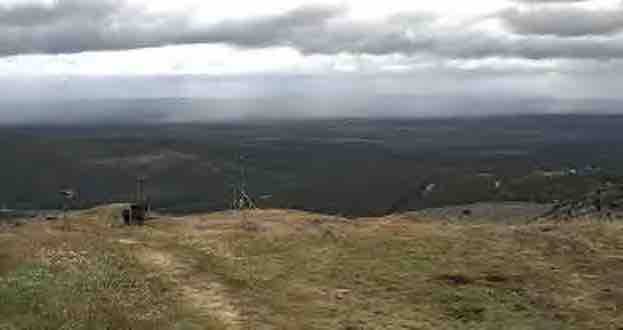
\includegraphics[width=8cm]{WebcamLapland.jpg}  
\caption{A webcam snapshot taken near a ski resort in Lapland.}
\label{fig:webcam_forestfire}
\end{center}
\end{figure}
A particular snapshot is characterized by the features $\vx$ and 
the label $y \in \labelspace=\{-1,1\}$ with $y=1$ if the snapshot 
shows a forest fire and $y=-1$ if there is no forest fire. We would 
like to find or learn a classifier $h(\vx)$ which takes the features $\vx$ 
as input and provides a classification according to 
\begin{equation} 
\label{equ_def_classification}
\hat{y} =  \begin{cases} 1 & \mbox{ if } h(\vx) \geq 0 \\ 
-1 & \mbox{ if } h(\vx) \leq 0. \end{cases} 
\end{equation} 

Ideally we would like to have $\hat{y} = y$ for any datapoint. 
This suggests to learn a hypothesis $h(\vx)$ by minimizing 
the $0/1$ loss
\begin{equation}
\label{equ_def_0_1}
\loss{(\vx,y)}{h} \defeq \begin{cases} 1 &\mbox{ if } y h(\vx) < 0 \\ 0 & \mbox{ else.} \end{cases}
\end{equation} 
Figure \ref{fig_class_loss} illustrates the $0/1$ loss \eqref{equ_def_0_1} 
for a datapoint with features $\vx$ and label $y=1$ as a function of 
the hypothesis $h$. For a given datapoint $(\vx,y)$ and hypothesis 
$h$, the $0/1$ loss is equal to zero if $\hat{y}=y$ (see \eqref{equ_def_classification}) 
and equal to one otherwise. 

The $0/1$ loss \eqref{equ_def_0_1} is conceptually appealing when 
datapoints are interpreted as realizations of i.i.d.\ random variables 
with underlying probability distribution $p(\vx,y)$. Given 
$\samplesize$ realizations $(\vx^{(\sampleidx)},y^{(\sampleidx)}) \big\}_{\sampleidx=1}^{\samplesize}$ 
of such i.i.d.\ random variables,
\begin{equation} 
\label{equ_0_1_approx_prob}
(1/\samplesize) \sum_{\sampleidx=1}^{\samplesize} \loss{(\vx^{(\sampleidx)},y^{(\sampleidx)})}{h} \approx \prob{ y \neq \hat{y} }
\end{equation} 
with high probability for sufficiently large sample size $\samplesize$. 
%The approximation \eqref{equ_0_1_approx_prob} is based on the fact 
%that the average of a large number of realizations of i.i.d.\ random 
%variables can be well approximated by their (common) mean or expectation. 
The precise formulation of the approximation \eqref{equ_0_1_approx_prob} 
is known as the ``law of large numbers'' \cite[Section 1]{BillingsleyProbMeasure}. 
We can apply the law of large numbers since the loss values $\loss{(\vx^{(\sampleidx)},y^{(\sampleidx)})}{h}$ 
are realizations of i.i.d.\ random variables. 

In view of \eqref{equ_0_1_approx_prob}, the $0/1$ loss seems 
a very natural choice for assessing the quality of a classifier 
if our goal is to enforce correct classification ($\hat{y}=y$). 
This appealing statistical property of the $0/1$ loss comes 
at the cost of high computational complexity. Indeed, for a 
given datapoint $(\vx,y)$, the $0/1$ loss \eqref{equ_def_0_1} 
is neither convex nor differentiable when viewed as a function 
of the classifier $h$. Thus, using the $0/1$ loss for binary 
classification problems typically involves advanced optimization 
methods for solving the resulting learning problem (see Section \ref{sec_NaiveBayes}). 

In order to ``cure'' the non-convexity of the $0/1$ loss we 
approximate it by a convex loss function. This convex 
approximation results in the {\bf hinge loss}
\begin{equation} 
\label{equ_hinge_loss}
\loss{(\vx,y)}{h} \defeq \max \{ 0 , 1 - y\cdot h(\vx) \}. 
\end{equation}
Figure \ref{fig_class_loss} depicts the hinge loss \eqref{equ_hinge_loss} 
as a function of the hypothesis $h(\vx)$. 
While the hinge loss avoids the non-convexity of the $0/1$ 
loss it still is a non-differentiable function of the classifier $h$. 

Section \ref{sec_LogReg} discusses the {\bf logistic loss} which is 
a differentiable loss function that is useful for classification problems. 
The logistic loss
\begin{equation} 
\label{equ_log_loss}
\loss{(\vx,y)}{h} \defeq  \log ( 1 + \exp(- y h(\vx))),
\end{equation}
is used within logistic regression to measure the usefulness of 
a linear hypothesis $h(\vx) = \vw^{T} \vx$. 

For a fixed feature vector $\vx$ and label $y$, both, the hinge 
and the logistic loss function are {\bf convex functions} of 
the hypothesis $h$. The logistic loss \eqref{equ_log_loss} 
depends {\bf smoothly} on $h$ such that we could define a derivative 
of the loss with respect to $h$. In contrast, the hinge loss 
\eqref{equ_hinge_loss} is {\bf non-smooth} which makes it 
more difficult to minimize. 

ML methods that use the logistic loss function, such 
as logistic regression in Section \ref{sec_LogReg}, can 
apply simple {\bf gradient descent methods} (see Chapter \ref{ch_GD}) 
to minimize the average loss. 

ML methods based on the hinge loss, such as those presented 
in Section \ref{sec_SVM}, must use more sophisticated optimization 
methods to learn a predictor by minimizing the loss (see Chapter \ref{ch_Optimization}).  
We cannot directly apply GD to minimize the hinge loss since 
it is not differentiable. However, we can apply a generalization of 
GD which is known as {\bf subgradient descent} \cite{CvxBubeck2015}. 
Loosely speaking, subgradient descent is obtained from GD 
by replacing the concept of a gradient with the concept 
of a subgradient. 


\hspace*{10mm}
\begin{center}
\begin{figure}[htbp]
    \begin{tikzpicture}
    	 \hspace*{-10mm}
          \begin{axis}
          [ylabel=$h(x)$,
              xlabel=$x$,grid, 
              axis x line=center,
  axis y line=center,
  xtick={-2,-1,...,2},
  ytick={0,1,...,2},
  xlabel={predictor $h(x)$},
  ylabel={loss $\mathcal{L}$},
  xlabel style={below right},
  ylabel style={above left},
  xmin=-4,
  xscale = 1.4, 
  xmax=4,
  ymin=-0.5,
  ymax=2.5
  ]
               \addplot [smooth, color=red, ultra thick] table [x=a, y=b, col sep=comma] {logloss.csv};    
                   \addplot [color=blue, ultra thick] table [x=a, y=b, col sep=comma] {hingeloss.csv};     
                   \addplot [color=black, ultra thick] table [x=a, y=b, col sep=comma] {zerooneloss.csv};     
                     \addplot[domain=-1:4, thin,dashed] {(x-1)^2};
       \end{axis}
          
     \node [right] at (10,5) { very confident in $\hat{y}\!=\!1 \Rightarrow$}; 
     \node [right,color=red] at (7,1.5) {logistic loss (for $y\!=\!1$)};
         \node [right] at (7,3) {squared error (for $y\!=\!1$)};
      \node [right,color=blue] at (4,4) {hinge loss (for $y\!=\!1)$};
      \node [left] at (2.5,3) {\bf $0/1$ loss (for $y\!=\!1)$};
     \node [left] at (2,5) {$\Leftarrow$ very confident in $\hat{y}\!=\!-1$};
     \end{tikzpicture}
     \vspace*{-10mm}
\caption{Three loss functions for assessing the quality of a hypothesis $h$ 
	which is used to classify a datapoint with true label $y=1$ according to \eqref{equ_def_classification}. 
	The more confident we are in a correct classification ($\hat{y}=1$), i.e, 
	the more positive $h(x)$, the smaller the loss. Each of the three loss 
	functions tends monotonically to $0$ for increasing $h(x)$.}
\label{fig_class_loss}
\end{figure}
\end{center}

Let us emphasize that, very much like the choice of features 
and hypothesis space, the question of which particular loss 
function to use within an ML method is a {\bf design choice}. 
The choice for the loss function should take into account the 
available computational resources and the statistical properties 
of the data (see Section \ref{sec_comp_stat_ERM}). If we do 
not have access to any labeled datapoint, we might not use 
the squared error loss for measuring the quality of a hypothesis. 

An important aspect guiding the choice of the loss function is the 
computational complexity of the resulting ML method. The basic 
idea behind ML methods is quite simple: learn (find) the particular 
hypothesis out of a given hypothesis space which yields the smallest 
(average) loss. Section \ref{sec_comp_stat_ERM} will discuss how  
the choice for the loss function influences the computational complexity 
of the resulting ML method. Some loss functions can be minimized using 
efficient iterative methods that will be discussed in Chapter \ref{ch_GD}. 


{\bf Empirical and Generalization Risk.} 
Many ML methods are based on a simple probabilistic model for the 
observed datapoints (i.i.d.). Using this assumption, we can define the 
average or generalization risk as the expectation of the loss. A large class 
of ML methods is based on approximating the expected value of the loss 
by an empirical (sample) average over a finite set of labeled datapoints which 
are we refer to as the training set. 

We define the empirical risk of some predictor when applied to labeled datapoints $\dataset=\big(\vx^{(1)},y^{(1)}\big),\ldots,\big(\vx^{(\samplesize)},y^{(\samplesize)}\big)$ 
as 
\begin{equation} 
\label{eq_def_emp_error_101}
\emperror(h|\dataset) = (1/\samplesize)\sum_{\sampleidx=1}^{\samplesize} \loss{(\vx^{(\sampleidx)},y^{(\sampleidx)})}{h}.  
\end{equation} 
To ease notational burden, if the dataset $\dataset$ is clear from the context, 
we use $\emperror(h)$. 

{\bf Regret.} In some application, we might have access to the 
predictions obtained from some reference methods or {\bf experts}. 
The quality of a hypothesis $h$ can then be measured via the 
difference between the loss incurred by its predictions 
$h(\vx)$ and the loss incurred by the predictions of the experts 
\cite{HazanOCO}. This difference is referred to as the {\bf regret}. 
This different measures how much we regret to have used the 
prediction $h(\vx)$ instead of having followed the prediction of the expert. 
The goal of regret minimization is to learn a hypothesis 
with small regret compared to all considered experts. 

The concept of regret minimization is useful when we do 
not make any probabilistic assumptions (such as i.i.d.) about 
the datapoints. Without a probabilistic model we cannot use 
the Bayes risk (of Bayes optimal estimator) as benchmark. 
Regret minimization techniques can be designed and analyzed 
without any such probabilistic model for the data \cite{PredictionLearningGames}. 
This approach replaces the Bayes risk with the regret relative to 
given reference predictors (experts) as the benchmark. 

{\bf Partial Feedback, ``Reward''.}  
Some applications involve datapoints whose labels are so 
difficult or costly to determine that we cannot assume to 
have any labeled data available. Without any labeled data, 
we cannot use the concept of a loss function to measure the 
quality of a prediction.\footnote{The evaluation of the loss function 
requires that the label value is known!} Instead we must use 
some other form of indirect feedback or ``reward'' that indicates 
the usefulness of a particular prediction \cite{PredictionLearningGames,SuttonEd2}. 

Consider the ML problem of predicting the optimal steering 
directions for a toy car. The prediction has to be recalculated 
for each new state of the toy car. ML methods can sense the 
state via a feature vector $\vx$ whose entries are pixel intensities of a 
snapshot. The goal is to learn a hypothesis map from the feature vector 
$\vx$ to a guess $\hat{y} = h(\vx)$ for the optimal steering direction $y$ (true label). 

In some applications, we might have no access to the true label of any 
datapoint. This means that we cannot evaluate the quality of a particular 
map based on the average loss on training data. Instead, we might have 
only some indirect signal about the loss incurred by the prediction 
$\hat{y}=h(\vx)$. Such a feedback signal, or reward, could be obtained 
by a distance sensor which measures the change in the distance 
between the car and its goal such as the charging station. 

\section{Putting Together the Pieces} 
\label{sec_putting_togehter_the_pieces}

To illustrate how ML methods combine particular design choices for 
data, model and loss, we consider datapoints characterized by a single 
numeric feature $x \in \mathbb{R}$ and a numeric label $y \in \mathbb{R}$. 
We assume to have access to $\samplesize$ labeled datapoints 
\begin{equation} 
\big(x^{(1)},y^{(1)}\big),\ldots, \big(x^{(\samplesize)},y^{(\samplesize)}\big)  \label{equ_labeled_data_putting_together}
\end{equation} 
for which we know the true label values $y^{(\sampleidx)}$. 

The assumption of knowing the exact true label values $y^{(\sampleidx)}$ 
for any datapoint is an idealization. We might often face labelling 
or measurement errors such that the observed labels are noisy 
versions of the true label. Later on, we will discuss techniques that allow ML 
methods to cope with noisy labels in Chapter \ref{ch_overfitting_regularization}. 

Our goal is to learn a predictor map $h(x)$ such that $h(x) \approx y$ 
for any datapoint. We require the predictor map to belong to 
the hypothesis space $\hypospace$ of linear predictors 
\begin{equation} 
\label{equ_def_lin_pred_intercept}
h^{(w_{0},w_{1})}(x) = w_{1} x + w_{0}. 
\end{equation}

The predictor \eqref{equ_def_lin_pred_intercept} is parameterized by the slope 
$w_{1}$ and the intercept (bias or offset) $w_{0}$. We indicate this by the 
notation $h^{(w_{0},w_{1})}$. A particular choice for $w_{1},w_{0}$ 
defines some linear predictor $h^{(w_{0},w_{1})}(x) = w_{1}x +w_{0}$. 

Let us use some linear predictor $h^{(w_{0},w_{1})}(x)$ to predict the labels of 
training datapoints. In general, the predictions $\hat{y}^{(\sampleidx)} = h^{(w_{0},w_{1})}\big(x^{(\sampleidx)}\big)$ 
will not be perfect and incur a non-zero prediction error $\hat{y}^{(\sampleidx)} - y^{(\sampleidx)}$ (see Figure \ref{fig_emp_error}).  

We measure the goodness of the predictor map $h^{(w_{0},w_{1})}$ 
using the average squared error loss (see \eqref{equ_squared_loss})
\begin{align}
\label{equ_def_cost_fun_putting_togheter}
f(w_{0},w_{1}) & \defeq (1/\samplesize) \sum_{\sampleidx=1}^{\samplesize} \big( y^{(\sampleidx)} - h^{(w_{0},w_{1})}(x^{(i)})  \big)^{2} \nonumber \\
& \stackrel{\eqref{equ_def_lin_pred_intercept}}{=}  (1/\samplesize) \sum_{\sampleidx=1}^{\samplesize} \big( y^{(\sampleidx)} - ( w_{1} x^{(i)} + w_{0}) \big)^{2}. 
\end{align}
The training error $f(w_{0},w_{1})$ is the average of the squared 
prediction errors incurred by the predictor $h^{(w_{0},w_{1})}(x)$ 
to the labeled datapoints \eqref{equ_labeled_data_putting_together}. 

It seems natural to learn a good predictor \eqref{equ_def_lin_pred_intercept} 
by choosing the weights $w_{0},w_{1}$ to minimize the training error 
\begin{equation}
\min_{w_{1},w_{0} \in \mathbb{R}} f(w_{0},w_{1}) \stackrel{\eqref{equ_def_cost_fun_putting_togheter}}{=} \min_{w_{1},w_{0} \in \mathbb{R}}   (1/\samplesize) \sum_{\sampleidx=1}^{\samplesize} \big( y^{(\sampleidx)} - ( w_{1} x^{(\sampleidx)} + w_{0}) \big)^{2}.
\end{equation} 

The optimal weights $w_{0}',w_{1}'$ are characterized by the 
{\bf zero-gradient condition},\footnote{A necessary and sufficient 
condition for $\vw'$ to minimize a convex differentiable function 
$f(\vw)$ is $\nabla f(\vw') = \mathbf{0}$ \cite[Sec.\ 4.2.3]{BoydConvexBook}.} 
\begin{equation}
\label{equ_zero_grad_condition_putting_together}
\frac{\partial f(w'_{0},w'_{1})}{\partial w_{0}} = 0 \mbox{, and }\frac{\partial f(w'_{0},w'_{1})}{\partial w_{1}} = 0. 
\end{equation} 
Inserting \eqref{equ_def_cost_fun_putting_togheter} into \eqref{equ_zero_grad_condition_putting_together} and 
by using basic rules for calculating derivatives, we obtain the 
following optimality conditions 
\begin{equation}
\label{equ_zero_grad_condition_putting_together_special_form}
 (1/\samplesize) \sum_{\sampleidx=1}^{\samplesize} \big( y^{(\sampleidx)} - ( w'_{1} x^{(\sampleidx)} + w'_{0}) \big)= 0 \mbox{, and } (1/\samplesize) \sum_{\sampleidx=1}^{\samplesize} x^{(\sampleidx)} \big( y^{(\sampleidx)} - ( w'_{1} x^{(\sampleidx)} + w'_{0}) \big) = 0. 
\end{equation} 

Any weights $w'_{0},w'_{1}$ that satisfy \eqref{equ_zero_grad_condition_putting_together_special_form} 
define a predictor $h^{(w'_{0},w'_{1})} = w'_{1}x + w'_{0}$ that 
is optimal in the sense of incurring minimum training error, 
$$f(w'_{0},w'_{1}) = \min_{w_{0},w_{1} \in \mathbb{R}} f(w_{0},w_{1}).$$

We find it convenient to rewrite the optimality condition \eqref{equ_zero_grad_condition_putting_together_special_form} 
using matrices and vectors. To this end, we first rewrite the 
predictor \eqref{equ_def_lin_pred_intercept} as 
$$ h(\vx) = \vw^{T} \vx \mbox{ with } \mathbf{w} = \big(w_{0},w_{1}\big)^{T}, \mathbf{x} = \big(1,x\big)^{T}.$$
Let us stack the feature vectors $\vx^{(\sampleidx)} = \big(1,x^{(\sampleidx)} \big)^{T}$ 
and labels $y^{(\sampleidx)}$ of training datapoints \eqref{equ_labeled_data_putting_together} 
into the feature matrix and label vector, 
\begin{equation}
\mX  = \big(\vx^{(1)},\ldots,\vx^{(\samplesize)}\big)^{T} \in \mathbb{R}^{\samplesize \times 2}, \vy = \big(y^{(1)},\ldots,y^{(\samplesize)}\big)^{T} \in \mathbb{R}^{\samplesize}. 
\end{equation} 
We can then reformulate \eqref{equ_zero_grad_condition_putting_together_special_form} as 
\begin{equation}
\label{equ_zero_grad_condition_putting_together_special_form_mtx}
\mX^{T} \big( \vy - \mX \vw' \big) = \mathbf{0}. 
\end{equation} 
The entries of any weight vector $\vw' = \big(w_{0}',w_{1}'\big)$ that satisfies 
\eqref{equ_zero_grad_condition_putting_together_special_form_mtx} are solutions to 
\eqref{equ_zero_grad_condition_putting_together_special_form}. 




\begin{figure}[htbp]
    \centering
   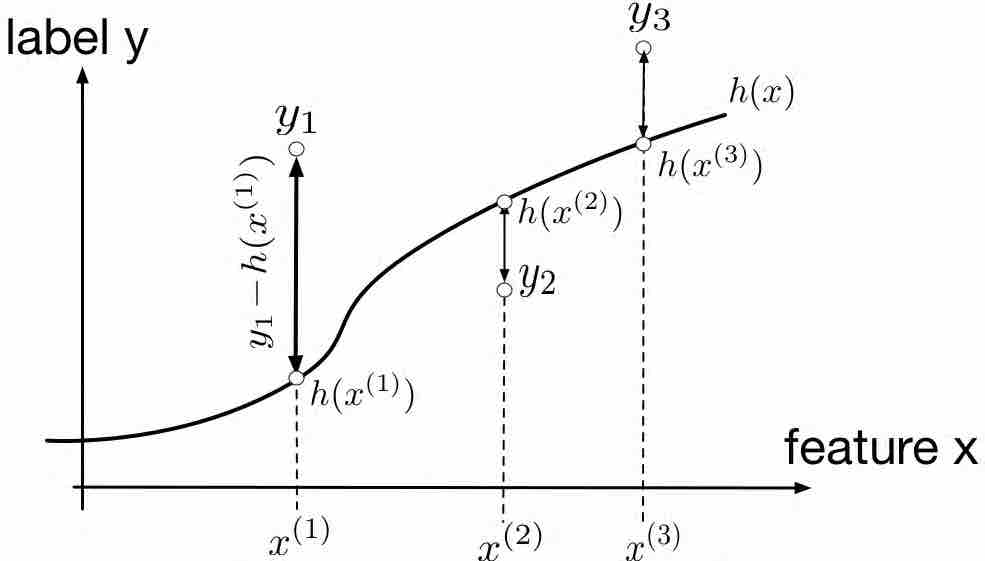
\includegraphics[width=0.7\textwidth]{EmpError.jpg}  
    \caption{We can evaluate the quality of a particular predictor $h \in \hypospace$ by measuring the 
    prediction error $y- h(x)$ obtained for a labeled datapoint $(x,y)$. }
   % For the \rumba\ application, these labeled datapoints could be a bunch of snapshots $\vz^{(\sampleidx)} = (\vx^{(\sampleidx)},y^{(\sampleidx)})$, for $\sampleidx=1,\ldots,\samplesize$, 
   % with feature vectors $\vx^{(\sampleidx)}$ and known $y$-coordinate $y^{(\sampleidx)}$ of 
    %the position where the $\sampleidx$-th snapshot has been taken.}
%    \caption{Hypothesis Map}\label{fig:Hypothesis Map}
  \label{fig_emp_error}
\end{figure}

\newpage
\section{Exercises} 

\subsection{ How Many Features?} 
\label{ex_compML_shazaam}
Consider the ML problem underlying a music information retrieval smartphone 
app \cite{ShazamPaper}. Such an app aims at identifying the song title based 
on a short audio recording of (an interpretation of) the song obtained via the 
microphone of a smartphone. Here, the feature vector $\vx$ represents the 
sampled audio signal and the label $y$ is a particular song title out of a huge 
music database. What is the length $\featuredim$ of the feature vector 
$\vx \in \mathbb{R}^{\featuredim}$ if its entries are the signal amplitudes of 
a $20$-second long recording which is sampled at a rate of $44$ kHz?


\subsection{Multilabel Prediction} 
\label{ex_ch2_multilabel}
Consider datapoints, each characterized by a feature vector $\vx \in \mathbb{R}^{10}$ and 
vector-valued labels $\vy \in \mathbb{R}^{30}$. Such vector-valued labels might be useful 
in multi-label classification problems. We might try to predict the label vector based on the 
features of a datapoint using a linear predictor map 
\begin{equation}
\label{equ_lin_predictor_multilabel}
\vh(\vx) = \mathbf{W} \mathbf{x} \mbox{ with some matrix } \mathbf{W} \in \mathbb{R}^{30 \times 10}. 
\end{equation} 
How many different linear predictors \eqref{equ_lin_predictor_multilabel} are there ? 
10, 30,40, infinite. 




\subsection{Average Squared Error Loss as Quadratic Form} 
\label{ex_2_0}
Consider linear hypothesis space consisting of linear maps parameterized by 
weights $\mathbf{w}$. We try to find the best linear map by minimizing the average 
squared error loss (empirical risk) incurred on some labeled training datapoints 
$(\vx^{(1)},y^{(1)}),(\vx^{(2)},y^{(2)}),\ldots,(\vx^{(\samplesize)},y^{(\samplesize)})$.  
Is it possible to write the resulting empirical risk, viewed as a function $f(\vw)$ as 
a convex quadratic form $f(\vw) = \vw^{T} \mathbf{C} \vw + \vb \vw + c$? If this 
is possible, how are the matrix $\mathbf{C}$, vector $\vb$ and constant $c$ related 
to the feature vectors and labels of the training data ? 


\subsection{Find Labeled Data for Given Empirical Risk} 
\label{ex_2_1}
Consider linear hypothesis space consisting of linear maps parameterized by 
weights $\mathbf{w}$. We try to find the best linear map by minimizing the average 
squared error loss (empirical risk) incurred on some labeled training datapoints. 
Assume we know the shape of the empirical risk as a function of the weight. 
Can you reconstruct the labeled training data that resulted in this empirical risk 
function? Is the resulting labeled training data unique or are there different training sets 
that could have resulted in the same empirical risk function? 
%% write down empirical risk as quadratic form f(w) = w^{T} X' X w + y^*y + 2*y'*X*w %%%% 

\subsection{Dummy Feature Instead of Intercept}
\label{sec_dummy_feature}
Show that any predictor of the form $h(x) = w_{1} x +w_{0}$ can be emulated by 
combining a feature map $x \mapsto \mathbf{z}$ with a predictor of the form $\mathbf{w}^{T} \mathbf{z}$. 

\subsection{Approximate Non-Linear Maps Using Indicator Functions for Feature Maps}
\label{ex_2_2}
Consider an ML application generating datapoints characterized by a scalar feature $x \in \mathbb{R}$ 
and numeric label $y \in \mathbb{R}$. We construct non-linear predictor maps by first mapping the 
feature $x$ to a new feature vector $\vz=(\phi_{1}(x),\phi_{2}(x),\phi_{3}(x),\phi_{4}(x))$. 
The components $\phi_{1}(x),\ldots,\phi_{4}(x)$ are indicator functions of intervals 
$[-10,-5), [-5,0),[0,5),[5,10]$. In particular, $\phi_{1}(x) = 1$ for $x \in [-10,-5)$ and $\phi_{1}(x)=0$ otherwise. 
We construct a hypothesis space $\hypospace_{1}$ by all maps of the form $\vw^{T}\vz$. 
Note that the map is a function of the feature $x$ since the feature vector $\vz$ is a function 
of $x$. Which of the following predictor maps belong to $\hypospace_{1}$?

\begin{minipage}{.5\textwidth} %
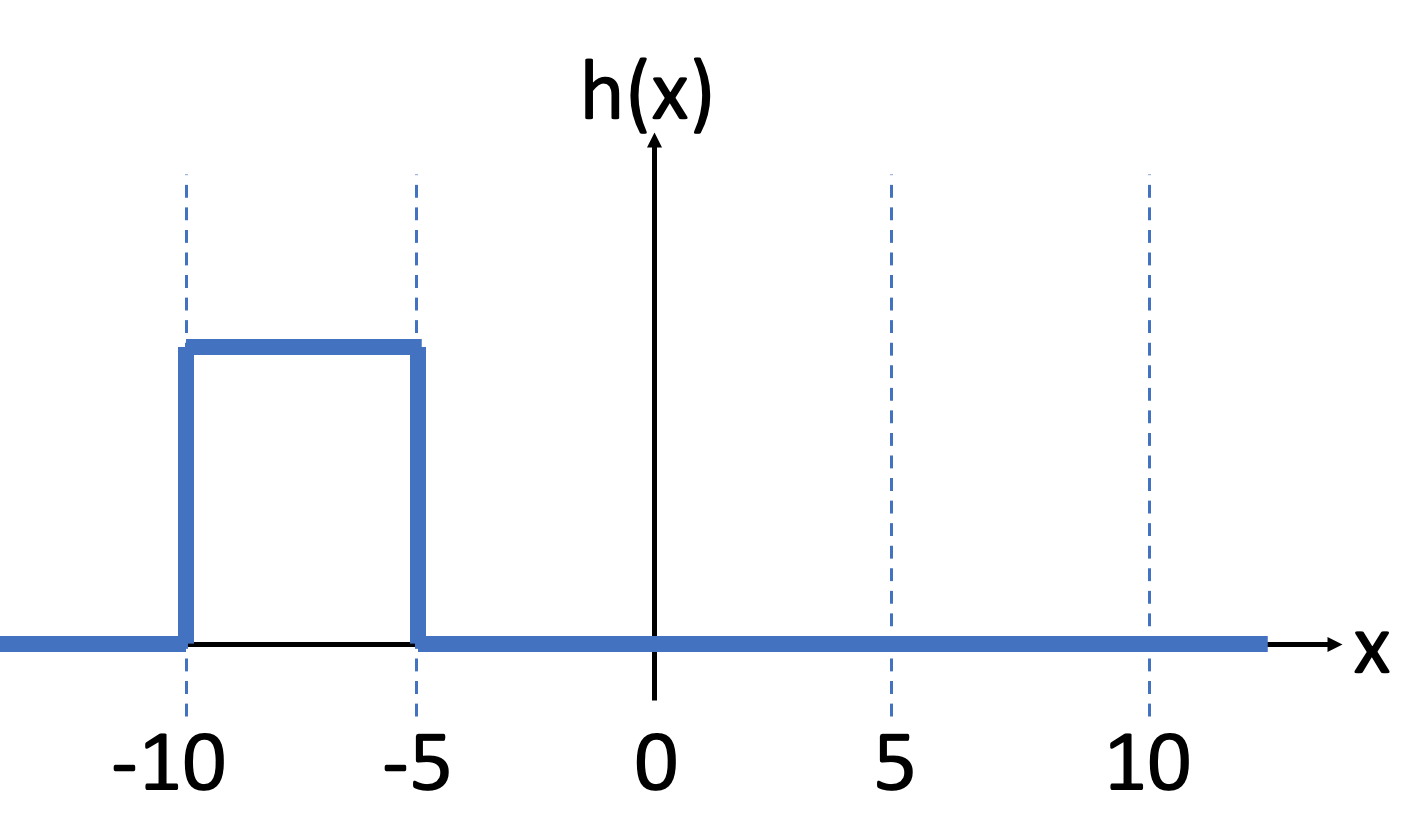
\includegraphics[width=4cm]{PiecewiseFun1.png}

(a)
\end{minipage} %
\begin{minipage}{.5\textwidth} %
	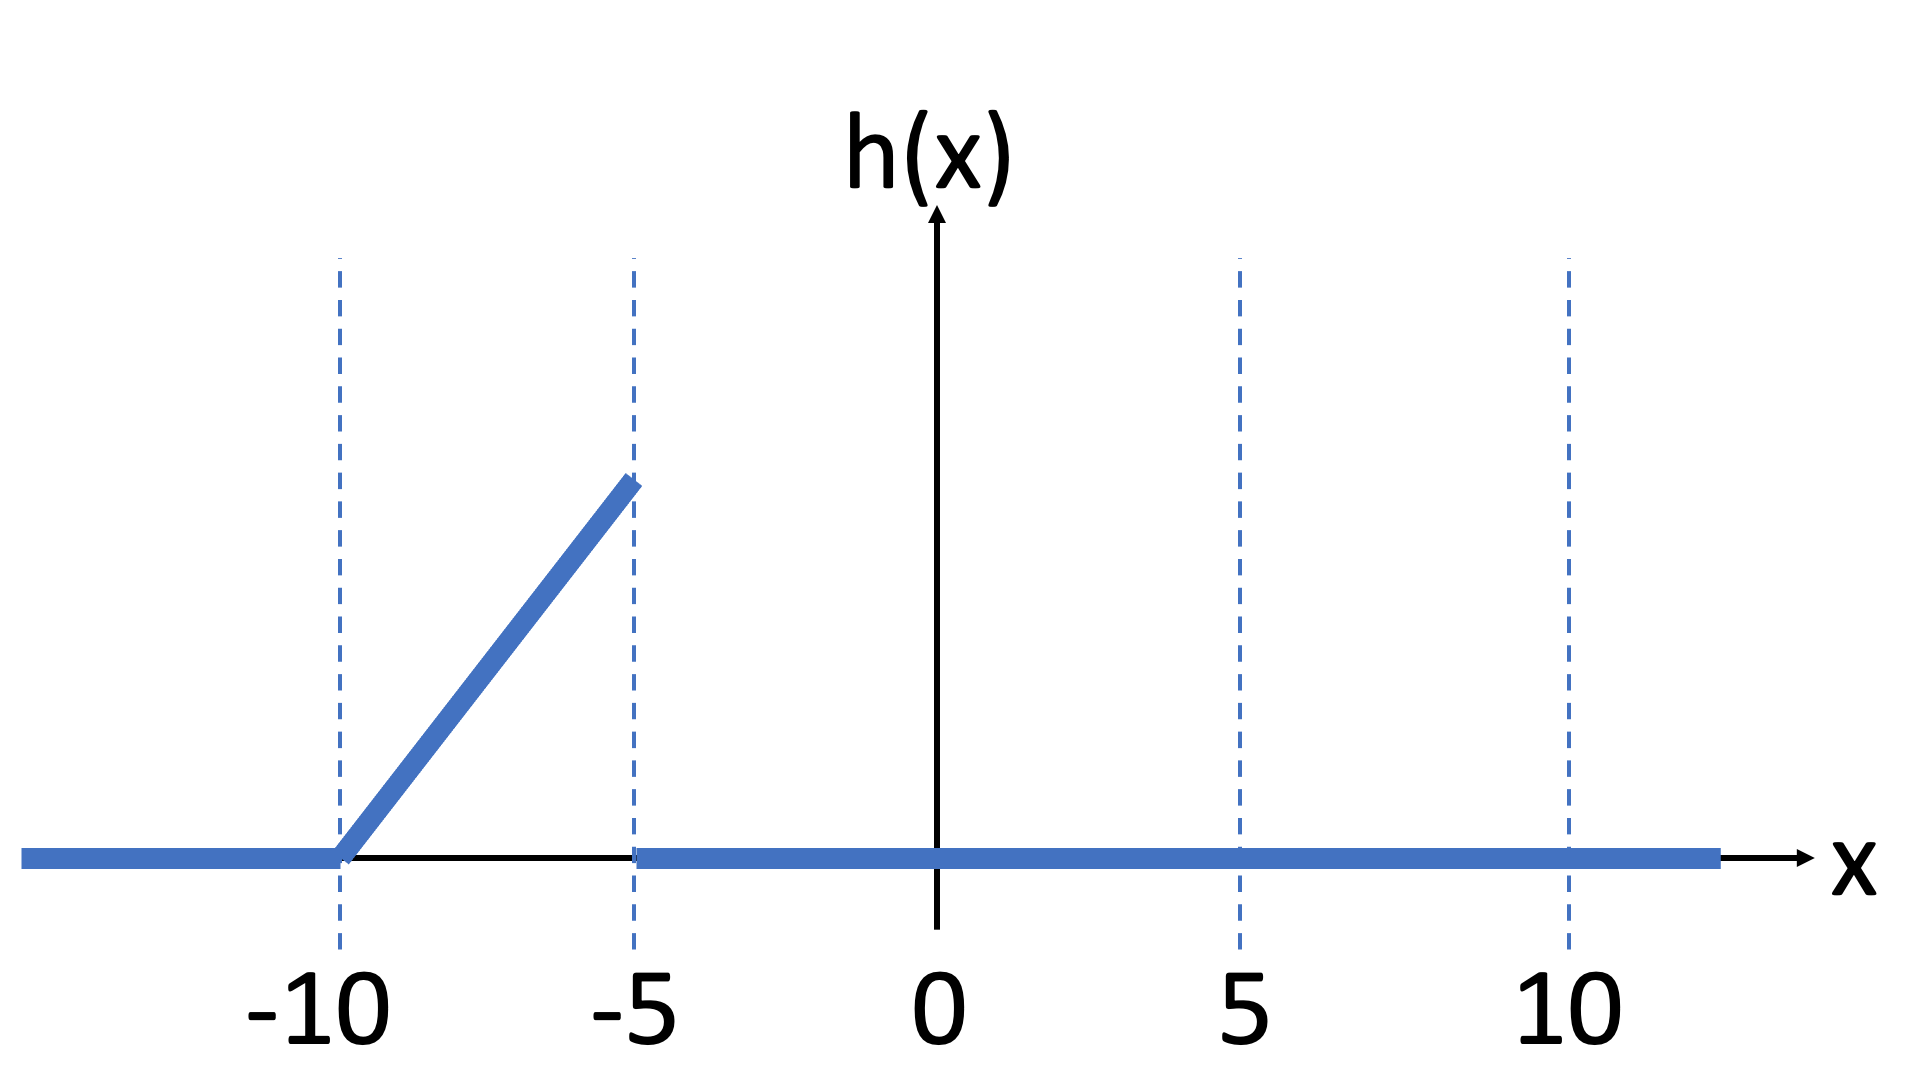
\includegraphics[width=4cm]{PiecewiseFun2.png}
	
(b)
\end{minipage}
 
 \subsection{Python Hypothesis Space}
 \label{ex_2_3}
 Consider the source codes below for five different Python functions that read 
 in the feature $x$ and return some prediction $\hat{y}$. How many elements 
 does the hypothesis space contain that is constituted by all maps $h(x)$ that 
 can be represented by one of those Python functions. 
 
  \subsection{A Lot of Features}
 \label{ex_2_toomanyfeatures}
In many application domains, we have access to a large number of features for 
each individual datapoint. Consider healthcare, where datapoints represent 
human patients. We could use all the measurements and diagnosis stored in 
the patient health record as features. When we use ML algorithms to 
analyse these datapoints, is it in general a good idea to use as much 
features as possible for datapoints ? 
 
  \subsection{Over-Parameterization}
 \label{ex_2_overparm}
Consider datapoints characterized by feature vectors $\vx \in \mathbb{R}^{2}$ and 
a numeric label $y \in \mathbb{R}$. We want to learn the best 
predictor out of the hypothesis space 
$$ \mathcal{H} = \big\{ h(\vx) = \vx^{T} \mathbf{A} \mathbf{w}: \mathbf{w} \in \mathcal{S} \}. $$
Here, we used the matrix 
$\mathbf{A} = \begin{pmatrix} 1 & -1 \\ -1 & 1 \end{pmatrix}$ and 
the set $$\mathcal{S} = \big\{ (1,1)^{T}, (2,2)^{T}, (-1,3)^{T}, (0,4)^{T} \big\} \subseteq \mathbb{R}^{2}.$$ 
What is the cardinality of $\mathcal{H}$, i.e., how many 
different predictor maps does $\mathcal{H}$ contain?
 
  \subsection{Squared Error Loss}
 \label{ex_2_4}
 Consider a hypothesis space $\hypospace$ constituted by three predictors $h_{1}(\cdot), h_{2}(\cdot),h_{3}(\cdot)$. 
 Each predictor $h_{j}(x)$ is a real-valued function of a real-valued argument $x$. Moreover, for each $j \in \{1,2,3\}$, 
 $h_{j}(x) = 0$ for all $x^2 \leq 1$. Can you tell which of these predictors is optimal in the sense of incurring the 
 smallest average squared error loss on the three (training) datapoints $(x=1/10,y=3)$, $(0,0)$ and $(1,-1)$. 
 
 \subsection{Classification Loss} 
 \label{ex_2_classif_loss}
 \begin{center}
 	\framebox[0.96\textwidth]{
 		\parbox{0.9\textwidth}{
 			{\bf Exercise.} How would Figure \ref{fig_class_loss} change if we consider the loss 
 			functions for a datapoint $z=(x,y)$ with known label $y=-1$?
 	}}
 \end{center}
 
 \subsection{Intercept Term}
 \label{ex_2_5}
 Linear regression models the relation between the label $y$ and feature $x$ of 
 a datapoint by $y = h(x) + e$ with some small additive term $e$. The predictor 
 map $h(x)$ is assumed to be linear $h(x) =w_1 x + w_0$. The weight $w_{0}$ is 
 sometimes referred to as the intercept (or bias) term. Assume we know for a given 
 linear predictor map its values $h(x)$ for $x=1$ and $x=3$. Can you determine 
 the weights $w_{1}$ and $w_{0}$ based on $h(1)$ and $h(3)$?
 
 \subsection{Picture Classification} 
 \label{ex_2_6}
Consider a huge collection of outdoor pictures 
you have taken during your last adventure 
trip. You want to organize these pictures as 
three categories (or classes) \emph{dog}, 
\emph{bird} and \emph{fish}. How could you  
formalize this task as a ML problem? 

 \subsection{Maximum Hypothesis Space} 
\label{ex_2_7}
Consider datapoints characterized by a single real-valued 
feature $x$ and a single real-valued label $y$. How large 
is the largest possible hypothesis space of predictor maps 
$h(x)$ that read in the feature value of a datapoint and 
deliver a real-valued prediction $\hat{y}=h(x)$ ? 

 \subsection{A Large but Finite Hypothesis Space} 
\label{ex_2_8}
Consider datapoints whose features are $10 \times 10$ 
black-and-white (bw) pixel images. Each datapoint is also 
characterized by a binary label $y \in \{0,1\}$. Consider the 
hypothesis space which is constituted by all maps that take 
a bw image as input and deliver a prediction for the label. 
How large is this hypothesis space? 

\subsection{Size of Linear Hypothesis Space} 
\label{ex_size_lin_hypospace} 
Consider a training set of $\samplesize$ datapoints with feature 
vectors $\vx^{(\sampleidx)} \in \mathbb{R}^{\featuredim}$ and 
numeric labels $y^{(1)},\ldots,y^{(\samplesize)}$. The feature vectors 
and label values of the training set are arbitrary except that we assume 
the feature matrix $\mathbf{X} = \big(\vx^{(1)},\ldots \big)$ is full rank. 
What condition on $\samplesize$ and $\featurelen$ guarantee that we 
can find a linear predictor $h(\vx) = \vw^{T} \vx$ that perfectly fits the 
training set, i.e., $y^{(1)} = h\big(\vx^{(1)} \big),\ldots, y^{(\samplesize)} = h\big(\vx^{(\samplesize)} \big)$. 


\newpage
\chapter{Some Examples} 
\label{ch_some_examples}
As discussed in Chapter \ref{ch_Elements_ML}, ML methods combine 
three main components: 
\begin{itemize} 
\item the data which is characterized by {\bf features} which can be computed 
or measured easily and {\bf labels} which represent high-level facts. 
\item a {\bf model} or {\bf hypothesis space} $\hypospace$ which consists of 
computationally feasible predictor maps $h \in \hypospace$. 
\item a {\bf loss function} to measure the quality of a particular predictor map $h$. 
\end{itemize} 
Each of these three components involves design choices for the data 
features and labels, the model and loss function. This chapter details 
the specific design choices used by some of the most popular ML 
methods. 

%A rough guideline for which of these methods to use for a given ML problem is depicted in Figure \ref{fig_python_cheat_sheet}.
%\begin{figure}[htbp]
%    \centering
%   \includegraphics[width=0.7\textwidth]{Cheat_Sheet.png}  
%    \caption{A simple guideline for choosing the ML method for a problem at hand.}
%%    \caption{Hypothesis Map}\label{fig:Hypothesis Map}
%  \label{fig_python_cheat_sheet}
%\end{figure}
\begin{figure}
	\resizebox{.9\textwidth}{!}{
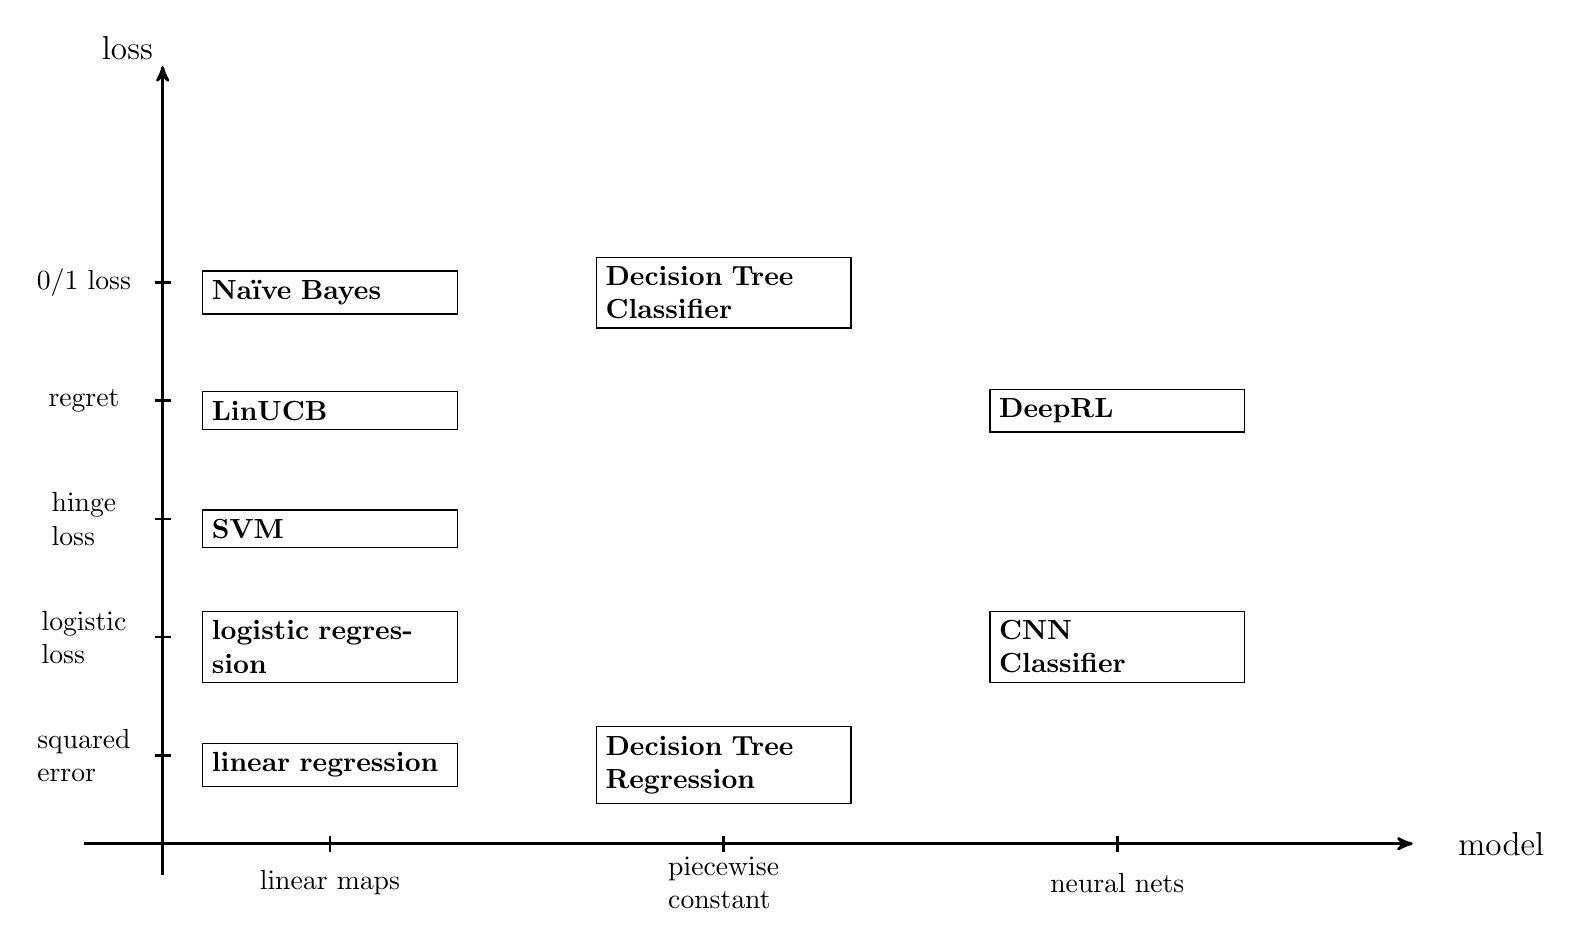
\begin{tikzpicture}[auto]
	\coordinate (OR) at (0.00, 0.0);
	\coordinate (RIGHT) at (16,0); 
	\coordinate (TOP) at (0.0,10) ; 
  %  \coordinate (MIDDLE) at (3,2) ; 
	\node[](a) at (OR) {};
    \node[](b) at (RIGHT) {};
    \node[](c) at (TOP) {};
    %\node[](c) at (TOP) {};
    \node[]  at  ($ (b) + (1,0) $)  {\large model};
    \node[above=1cm of OR] (sqerror) {} ;
    \node[above=2.5cm of OR] (logloss) {} ;
     \node[above=4cm of OR] (hingeloss) {} ;
    \node[above=5.5cm of OR] (regret) {} ;
        \node[above=7cm of OR] (zeroone) {} ;
    \node[align=left]  at  ($ (logloss) - (1,0) $)  {logistic\\loss};
    \node[align=left]  at  ($ (sqerror) - (1,0) $)  {squared\\error};
    \node[align=left]  at  ($ (hingeloss) - (1,0) $)  {hinge\\loss};
    \node[align=left]  at  ($ (regret) - (1,0) $)  {regret};
     \node[align=left]  at  ($ (zeroone) - (1,0) $)  {$0/1$ loss};
    \node[anchor=east]  at  ($ (c) + (0,0.1) $)  {\large loss};
    \node[right=2cm of OR] (linpred) {} ;
    \node[right=12cm of OR] (neuralnets) {} ;
    \node[right=7cm of OR] (piecewise) {} ;
    \node[]  at  ($ (linpred) - (0,0.5) $)  {linear maps};
    \node[]  at  ($ (neuralnets) - (0,0.5) $)  {neural nets};
    \node[align=left]  at  ($ (piecewise) - (0,0.5) $)  {piecewise \\ constant};
    \node[draw,text width=3cm]  at  ($ (linpred) + (0,1) $)  {\bf linear regression};
    \node[draw,text width=3cm]  at  ($ (linpred) + (0,2.5) $)  {\bf logistic regression};
    \node[draw,text width=3cm]  at  ($ (linpred) + (0,4) $)  {\bf SVM};
    \node[draw,text width=3cm]  at  ($ (linpred) + (0,5.5) $)  {\bf LinUCB};
    \node[draw,text width=3cm]  at  ($ (linpred) + (0,7) $)  {\bf Na\"ive Bayes};
    \node[draw,text width=3cm,,align=left]  at  ($ (piecewise) + (0,7) $)  {\bf Decision Tree \\ Classifier};
    \node[draw,text width=3cm,,align=left]  at  ($ (piecewise) + (0,1) $)  {\bf Decision Tree \\ Regression};
    \node[draw,text width=3cm]  at  ($ (neuralnets) + (0,5.5) $)  {\bf DeepRL};
    \node[draw,text width=3cm,align=left]  at  ($ (neuralnets) + (0,2.5) $)  {\bf CNN\\  Classifier};
    \draw[black,line width=1] ($ (linpred) - (0,0.1) $) to ($ (linpred) + (0,0.1) $) ;
    \draw[black,line width=1] ($ (neuralnets) - (0,0.1) $) to ($ (neuralnets) + (0,0.1) $) ;
    \draw[black,line width=1] ($ (piecewise) - (0,0.1) $) to ($ (piecewise) + (0,0.1) $) ;
    \draw[black,line width=1] ($ (sqerror) - (0.1,0) $) to ($ (sqerror) + (0.1,0) $) ;
    \draw[black,line width=1] ($ (logloss) - (0.1,0) $) to ($ (logloss) + (0.1,0) $) ;
    \draw[black,line width=1] ($ (hingeloss) - (0.1,0) $) to ($ (hingeloss) + (0.1,0) $) ;
    \draw[black,line width=1] ($ (regret) - (0.1,0) $) to ($ (regret) + (0.1,0) $) ;
    \draw[black,line width=1] ($ (zeroone) - (0.1,0) $) to ($ (zeroone) + (0.1,0) $) ;
    \draw[->,black,line width=1] ($ (a) - (1,0) $) to (b);
    \draw[->,black,line width=1] ($ (a) - (0,0.4) $) to (c);
\end{tikzpicture}
	}
\caption{ML methods fit a model to data by minimizing a loss function. Different ML 
methods use different design choices for model, data and loss.}
\end{figure}


\section{Linear Regression} 
\label{sec_lin_regression}

Linear regression uses the feature space $\featurespace\!=\!\mathbb{R}^{\featuredim}$, 
label space $\labelspace\!=\!\mathbb{R}$ and the linear hypothesis space 
\begin{align}
\label{equ_lin_hypospace}
\hypospace^{(\featuredim)} & = \{ h^{(\vw)}: \mathbb{R}^{\featuredim}\!\rightarrow\!\mathbb{R}: h^{(\vw)}(\vx)\!=\!\vw^{T} \vx \mbox{ with some} \nonumber \\ 
& \mbox{ weight vector } \vw \in \mathbb{R}^{\featuredim} \}.
\end{align}  
The quality of a particular predictor $h^{(\vw)}$ is measured by 
the squared error loss \eqref{equ_squared_loss}. Using labeled 
training data $\dataset =\{ (\vx^{(\sampleidx)},y^{(\sampleidx)}) \}_{\sampleidx=1}^{\samplesize}$, 
linear regression learns a predictor $\hat{h}$ which minimizes 
the average squared error loss, or {\bf mean squared error}, (see \eqref{equ_squared_loss})
\begin{align} 
\label{equ_opt_pred_linreg}
\hat{h} & = \argmin_{h \in \hypospace^{(\featuredim)}  }\emperror(h|\dataset)  \\ \nonumber 
& \stackrel{\eqref{eq_def_emp_error_101}}{=} \argmin_{h \in \hypospace^{(\featuredim)}  }  (1/\samplesize) \sum_{\sampleidx=1}^{\samplesize} (y^{(\sampleidx)} - h(\vx^{(\sampleidx)}))^{2}.
\end{align} 

Since the hypothesis space $\hypospace^{(\featuredim)} $ is 
parameterized by the weight vector $\vw$ (see \eqref{equ_lin_hypospace}), 
we can rewrite \eqref{equ_opt_pred_linreg} as an optimization 
problem directly over the weight vector $\vw$: 
\begin{align} 
\label{equ_opt_weight_vector_linreg_weight}
\vw_{\rm opt} &  = \argmin_{\vw \in \mathbb{R}^{\featuredim}} (1/\samplesize) \sum_{\sampleidx=1}^{\samplesize} (y^{(\sampleidx)} - h^{(\vw)}(\vx^{(\sampleidx)}))^{2} \nonumber \\
& \stackrel{h^{(\mathbf{w})}(\vx) = \vw^{T} \vx}{=} \argmin_{\vw \in \mathbb{R}^{\featuredim}} (1/\samplesize) \sum_{\sampleidx=1}^{\samplesize} (y^{(\sampleidx)} - \vw^{T} \vx^{(\sampleidx)})^{2}.
\end{align} 
The optimization problems \eqref{equ_opt_pred_linreg} and \eqref{equ_opt_weight_vector_linreg_weight} 
are equivalent in the following sense: Any optimal weight vector $\vw_{\rm opt}$ which solves 
\eqref{equ_opt_weight_vector_linreg_weight}, can be used to 
construct an optimal predictor $\hat{h}$, which solves 
\eqref{equ_opt_pred_linreg}, via $\hat{h}(\vx) = h^{(\vw_{\rm opt})}(\vx) = \vw_{\rm opt}^{T} \vx$. 


\section{Polynomial Regression} 
\label{sec_polynomial_regression}

%??????
%Implementing polynomial regression (task 3.4) really helped me understand what it is all about. 
%I did not quite grasp the concept from the course book, but in the exercise 3.4 description there was an image of the 
%feature matrix with the initial feature raised to the nth power, where n ranges from 0 to d -1, that really made it click for me.??????

Consider an ML problem involving datapoints which are characterized by a 
single numeric feature $x \in  \mathbb{R}$ (the feature space is $\featurespace= \mathbb{R}$) 
and a numeric label $y \in \mathbb{R}$ (the label space is $\labelspace= \mathbb{R}$). 
We observe a bunch of labeled datapoints which are depicted in Figure \ref{fig_scatterplot_poly}. 

\begin{figure}[htbp]
\begin{center}
\begin{tikzpicture}[scale=0.8]
    \begin{axis}[
            axis x line=middle,
            axis y line=middle,
              ylabel near ticks,
    xlabel near ticks,
            enlarge y limits=true,
            %xmin=0, xmax=2150,
            %ymin=0, ymax=600,
            width=10cm, height=8cm,     % size of the image
            grid = major,
            grid style={dashed, gray!30},
            ylabel=label $y$,
            xlabel=feature $x$,
       %     legend style={at={(0.1,-0.1)}, anchor=north}
         ]        
          \addplot[only marks] table [x=BTCNorm, y=ETHNorm, col sep = comma] {CryptoScatter.csv};
          %the code below is added via @Peter's comment.
        %  \addplot[only marks] table [col sep = comma,y={create col/linear regression={y=column 2}}]{table3.csv};
    \end{axis}
\end{tikzpicture}
\end{center}
\caption{A scatterplot of some datapoints $(x^{(\sampleidx)},y^{(\sampleidx)})$.} 
\label{fig_scatterplot_poly}
\end{figure}

Figure \ref{fig_scatterplot_poly} suggests that the relation $x \mapsto y$ between feature 
$x$ and label $y$ is highly non-linear. For such non-linear relations between features and 
labels it is useful to consider a hypothesis space which is constituted by
 polynomial functions
\begin{align}
\label{equ_def_poly_hyposapce}
\hypospace^{(\featuredim)}_{\rm poly}& = \{ h^{(\vw)}: \mathbb{R} \rightarrow \mathbb{R}: h^{(\vw)}(x) = \sum_{r=1}^{\featuredim+1} w_{r} x^{r-1} \mbox{, with } \nonumber \\ 
& \mbox{ some } \vw\!=\!(w_{1},\ldots,w_{\featuredim+1})^{T}\!\in\!\mathbb{R}^{\featuredim+1} \}. 
\end{align}
We can approximate any non-linear relation $y\!=\!h(x)$ with any desired level of 
accuracy using a polynomial $\sum_{r=1}^{\featuredim+1} w_{r} x^{r-1}$ of sufficiently large 
degree $\featuredim$.\footnote{The precise formulation of this statement is known as the 
``Stone-Weierstrass Theorem'' \cite[Thm. 7.26]{RudinBookPrinciplesMatheAnalysis}.}

As for linear regression (see Section \ref{sec_lin_regression}), we measure the quality 
of a predictor by the squared error loss \eqref{equ_squared_loss}. Based on labeled 
training data $\dataset =\{ (x^{(\sampleidx)},y^{(\sampleidx)}) \}_{\sampleidx=1}^{\samplesize}$, 
with scalar features $x^{(\sampleidx)}$ and labels $y^{(\sampleidx)}$, polynomial regression amounts to 
minimizing the average squared error loss (mean squared error) (see \eqref{equ_squared_loss}):
\begin{equation} 
\label{opt_hypo_poly}
\min_{h \in \hypospace_{\rm poly}^{(\featuredim)} } (1/\samplesize) \sum_{\sampleidx=1}^{\samplesize} (y^{(\sampleidx)} - h^{(\mathbf{w})}(x^{(\sampleidx)}))^{2}.
\end{equation} 

It is useful to interpret polynomial regression as a combination 
of a feature map (transformation) (see Section \ref{sec_feature_space}) 
and linear regression (see Section \ref{sec_lin_regression}). Indeed, 
any polynomial predictor $h^{(\vw)} \in \hypospace_{\rm poly}^{(\featuredim)}$ 
is obtained as a concatenation of the feature map  
\begin{equation}
\label{equ_poly_feature_map} 
\phi(x) \mapsto (1,x,\ldots,x^{\featuredim})^{T} \in \mathbb{R}^{\featuredim+1}
\end{equation}
with some linear map $g^{(\vw)}: \mathbb{R}^{\featuredim+1} \rightarrow \mathbb{R}: \vx \mapsto \vw^{T} \vx$, i.e., 
\begin{equation}
\label{equ_concact_phi_g_poly}
h^{(\vw)}(x) = g^{(\vw)}(\phi(x)). 
\end{equation}

Thus, we can implement polynomial regression by first applying 
the feature map $\featuremap$ (see \eqref{equ_poly_feature_map}) to 
the scalar features $x^{(\sampleidx)}$, resulting in the transformed 
feature vectors 
\begin{equation} 
\label{equ_def_poly_feature_vectors}
\vx^{(\sampleidx)} = \featuremap \big(x^{(\sampleidx)}\big) = \big(1,x^{(\sampleidx)},\ldots,\big( x^{(\sampleidx)} \big)^{\featuredim} \big)^{T} \in \mathbb{R}^{\featuredim+1}, 
\end{equation} 
and then applying linear regression  (see Section \ref{sec_lin_regression}) 
to these new feature vectors. By inserting \eqref{equ_concact_phi_g_poly} 
into \eqref{opt_hypo_poly}, we end up with a linear regression problem 
\eqref{equ_opt_weight_vector_linreg_weight} with feature vectors \eqref{equ_def_poly_feature_vectors}. 
Thus, while a predictor $h^{(\vw)} \in \hypospace_{\rm poly}^{(\featuredim)}$ 
is a non-linear function $h^{(\vw)}(x)$ of the original feature $x$, it is a linear 
function, given explicitly by $g^{(\vw)}(\vx) = \vw^{T}\vx$ (see \eqref{equ_concact_phi_g_poly}), 
of the transformed features $\vx$ \eqref{equ_def_poly_feature_vectors}. 

\section{Least Absolute Deviation Regression}
\label{sec_lad}

Learning a linear predictor by minimizing the average squared error loss incurred 
on training data is not robust against outliers. This sensitivity to outliers is rooted 
in the properties of the squared error loss $(\hat{y} - y)^{2}$. Minimizing the 
average squared error forces the resulting predictor $\hat{y}$ to not be too far 
away from any datapoint. However, it might be useful to tolerate a large prediction 
error $\hat{y}-y$ for few datapoints if they can be considered as outliers. 

Replacing the squared loss with a different loss function can 
make the learning robust against few outliers. One such robust 
loss function is the {\bf Huber loss} \cite{HuberRobustBook}
\begin{equation}
\loss{y}{\hat{y}} = \begin{cases} (1/2) (y-\hat{y})^{2} & \mbox{ for } |y-\hat{y}| \leq   \varepsilon \\ 
\varepsilon(|y-\hat{y}| - \varepsilon/2) & \mbox{ else. }\end{cases}
\end{equation}

The Huber loss contains a parameter $\epsilon$, which has to 
be adapted to the application at hand. The Huber loss is robust 
to outliers since the corresponding (large) prediction errors 
$y - \hat{y}$ are not squared. Outliers have a smaller effect 
on the average Huber loss over the entire dataset. 

The Huber loss contains two important special cases. 
The first special case occurs when $\varepsilon$ 
is chosen to be very large, such that the condition 
$|y-\hat{y}| \leq \varepsilon$ is satisfied for most 
datapoints. In this case, the Huber loss resembles 
the squared error loss $(y-\hat{y})^{2}$ (up to a scaling factor $1/2$). 

The second special case occurs when $\varepsilon$ is chosen 
to be very small (close to $0$) such that the condition $|y-\hat{y}| \leq \varepsilon$ 
is almost never satisfied. In this case, the Huber loss is equivalent 
to the absolute loss $|y - \hat{y}|$ scaled by a factor $\varepsilon$.

\section{The Lasso}
\label{sec_lasso}
We will see in Chapter \ref{ch_validation_selection} that linear 
regression (see Section \ref{sec_lin_regression}) does not work 
well for datapoints having more features than the number of 
training datapoints (this is the high-dimensional regime). 
One approach to avoid overfitting is to modify the squared error 
loss \eqref{equ_squared_loss} by taking into account the weight 
vector of the linear predictor $h(\vx) = \vw^{T}\vx$. 

The Least Absolute Shrinkage and Selection Operator (Lasso) is 
obtained from linear regression by replacing the squared error loss 
with the regularized loss 
\begin{equation}
\loss{(\vx,y)}{h^{(\vw)}} = (y-\vw^{T}\vx)^{2} + \alpha \| \vw \|_{1}. 
\end{equation}
The choice for the tuning parameter $\alpha$ can be guided 
by using a probabilistic model, 
$$ y = \overline{\vw}^{T} \vx + \varepsilon.$$ 
Here, $\overline{\vw}$ denotes some true underlying weight vector 
and $\varepsilon$ is as a random variable. 

Appropriate values for $\alpha$ can then be determined based 
on the variance of the noise, the number of non-zero entries in 
$\overline{\vw}$ and a lower bound on the non-zero values. 
Another option for choosing the value $\alpha$ is to try out different 
candidate values and pick the one resulting in smallest validation 
loss (see Section \ref{sec_validate_predictor}). 


\section{Gaussian Basis Regression}
\label{sec_linbasreg}
As discussed in Section \ref{sec_polynomial_regression}, we can 
extend the basic linear regression problem by first transforming 
the features $x$ using a vector-valued feature map $\phi: \mathbb{R} \rightarrow \mathbb{R}^{\featuredim}$ 
and then applying a weight vector $\vw$ to the transformed 
features $\phi(x)$. For polynomial regression, the feature map 
is constructed using powers $x^{l}$ of the scalar feature $x$. 

It is possible to use other functions, different from polynomials, 
to construct the feature map $\phi$. We can extend linear regression 
using an arbitrary feature map 
\begin{equation} 
\featuremap(x) = (\basisfunc_{1}(x),\ldots,\basisfunc_{\featuredim}(x))^{T}  
\end{equation} 
with the scalar maps $\basisfunc_{j}: \mathbb{R} \rightarrow \mathbb{R}$ which 
are referred to as {\bf basis functions}. The choice of basis functions 
depends heavily on the particular application and the underlying relation 
between features and labels of the observed datapoints. The basis 
functions underlying polynomial regression are $\basisfunc_{j}(x)= x^{j}$. 

Another popular choice for the basis functions are ``Gaussians'' 
\begin{equation} 
\label{equ_basis_Gaussian}
\phi_{\sigma,\mu}(x) = \exp(-(1/(2\sigma^{2})) (x\!-\!\mu)^{2}). 
\end{equation}
The family \eqref{equ_basis_Gaussian} of maps is parameterized by 
the variance $\sigma^{2}$ and the mean (shift) $\mu$. We obtain 
{\bf Gaussian basis linear regression} by combining 
the feature map 
\begin{equation} 
\phi(x) = \big (\phi_{\sigma_{1},\mu_{1}}(x) ,\ldots,\phi_{\sigma_{\featuredim},\mu_{\featuredim}}(x) \big)^{T} 
\end{equation}
with linear regression (see Figure \ref{fig_lin_bas_expansion}). The resulting hypothesis space is then
\begin{align}
\label{equ_def_Gauss_hypospace}
\hypospace^{(\featuredim)}_{\rm Gauss} & = \{ h^{(\vw)}: \mathbb{R} \rightarrow \mathbb{R}: h^{(\vw)}(x)\!=\!\sum_{j=1}^{\featuredim}  w_{j}\phi_{\sigma_{j},\mu_{j}}(x) \nonumber \\
& \mbox{ with weights } \vw=(w_{1},\ldots,w_{\featuredim})^{T} \in \mathbb{R}^{\featuredim}\}.
\end{align}

Different choices for the variance $\sigma^{2}$ and shifts $\mu_{j}$ 
of the Gaussian function in \eqref{equ_basis_Gaussian} results in 
different hypothesis spaces $\hypospace_{\rm Gauss}$. Chapter \ref{sec_modsel} 
will discuss model selection techniques that allow to find useful values 
for these parameters.

The hypotheses of \eqref{equ_def_Gauss_hypospace} are parameterized 
by a weight vector $\vw \in \mathbb{R}^{\featuredim}$. Each hypothesis 
 in $\hypospace_{\rm Gauss}$ corresponds to a particular choice 
for the weight vector $\vw$. Thus, instead of searching over $\hypospace_{\rm Gauss}$ 
to find a good hypothesis, we can search over $\mathbb{R}^{\featuredim}$.

%Note that choosing the variance $\sigma^{2}$ of the Gaussian basis functions \eqref{equ_basis_Gaussian} small and using a large number of 
%regular spaced Gaussian basis functions we can approximate well any sufficiently regular function (which is not changing too rapidly). 
%Here, $\sigma^{2}$ and $\mu_{1},\ldots,\mu_{\featuredim}$ are design parameters which have to be chosen suitably. 

\begin{figure}[htbp]
\begin{center}
    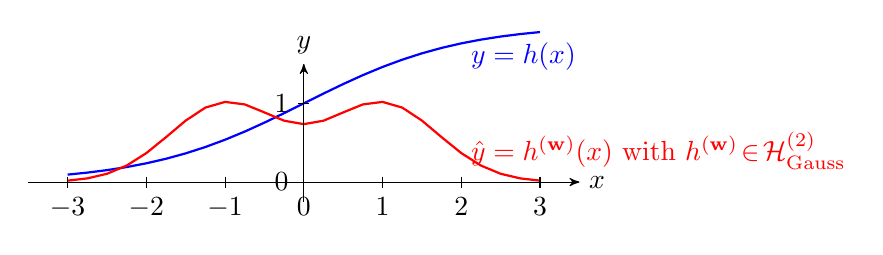
\begin{tikzpicture}
       %   \begin{axis}
       %   [ylabel=$h(x)$,
         %     xlabel=$x$,grid]
             %  \addplot table [x=a, y=b, col sep=comma] {data.csv};      
                 \draw[blue,  thick, domain=-3:3] plot (\x, {2/(1+exp(-\x))});
                  \draw[red,  thick, domain=-3:3] plot (\x,  {exp(-(\x+1)^2)+exp(-(\x-1)^2)}) ;
                  \node [red,right] at (2,0.4) {$\hat{y}=h^{(\vw)}(x)$ with $h^{(\vw)} \!\in\!\hypospace^{(2)}_{\rm Gauss}$} ; 
                   \node [blue,right] at (2,1.6) {$y=h(x)$} ; 
              %   \draw[blue,  thick, domain=-1:0] plot (\x,  {1+\x}); 
                % \draw[blue,  thick, domain=0:1] plot (\x,  {1-\x});    
                 %  \draw[blue,  thick, domain=1:3] plot (\x,  {0});           
          \draw[->] (-3.5,0) -- (3.5,0) node[right] {$x$};
   \draw[->] (0,-0.25) -- (0,1.5) node[above] {$y$};
           %      \draw[dashed, thick, domain=1:3.6] plot (\x,  {\x - 1}) node[right] {$ f(\vw_{0})\!+\!(\vw\!-\!\vw_{0})^{T} \nabla f(\vw_{0})$};
                    \foreach \y/\ytext in {0/0, 1/1}
    \draw[shift={(0,\y)}] (2pt,0pt) -- (-2pt,0pt) node[left] {$\ytext$};  
                        \foreach \x/\xtext in {-3/-3,-2/-2,-1/-1,0/0,1/1, 2/2,3/3}
    \draw[shift={(\x,0)}] (0pt,2pt) -- (0pt,-2pt) node[below] {$\xtext$};  
       %   \end{axis}
     \end{tikzpicture}
     \vspace*{-10mm}
\end{center}\caption{The true relation $x \mapsto y=h(x)$ (blue) between feature $x$ and label $y$ is highly non-linear. We might predict 
the label using a non-linear predictor $\hat{y}=h^{(\vw)}(x)$ with some weight vector $\vw \in \mathbb{R}^{2}$ and $h^{(\vw)} \!\in\!\hypospace^{(2)}_{\rm Gauss}$.} 
\label{fig_lin_bas_expansion}
\end{figure}

\begin{center}
\framebox[0.96\textwidth]{
 \parbox{0.9\textwidth}{
{\bf Exercise.} Try to approximate the hypothesis map depicted in Figure \ref{fig_triangle} by an element of $\hypospace_{\rm Gauss}$ (see \eqref{equ_def_Gauss_hypospace}) 
using $\sigma=1/10$, $\featuredim=10$ and $\mu_{j} = -1 + (2j/10)$. 
}}
\end{center}



\section{Logistic Regression} 
\label{sec_LogReg}

Logistic regression is a method for classifying datapoints which 
are characterized by feature vectors $\mathbf{x} \in \mathbb{R}^{\featuredim}$ 
(feature space $\featurespace=\mathbb{R}^{\featuredim}$) 
according to two categories which are encoded by a label $y$. 

It will be convenient to use the label space $\labelspace = \mathbb{R}$ 
and encode the two label values as $y=1$ and $y=-1$. Logistic regression 
learns a predictor out of the hypothesis space $\hypospace^{(\featuredim)}$ 
(see \eqref{equ_lin_hypospace}).\footnote{It is important to note that logistic 
regression can be used with an arbitrary label space which contains 
two different elements. Another popular choice for the label space is $\labelspace=\{0,1\}$.} 
Note that the hypothesis space is the same as used in linear regression (see Section \ref{sec_lin_regression}). 

At first sight, it seems wasteful to use a linear hypothesis $h(\vx) = \vw^T \vx$, 
with some weight vector $\vw \in \mathbb{R}^{\featuredim}$, to predict a 
binary label $y$. Indeed, while the prediction $h(\vx)$ can take any real number, 
the label $y \in \{-1,1\}$ takes on only one of the two real numbers $1$ and $-1$. 

It turns out that even for binary labels it is quite useful to use 
a hypothesis map $h$ which can take on arbitrary real numbers. 
We can always obtain a predicted label $\hat{y} \in \{-1,1\}$ by comparing 
hypothesis value $h(\vx)$ with a threshold. A datapoint with features $\vx$, 
is classified as $\hat{y}=1$ if $h(\vx)\geq 0$ and $\hat{y}=-1$ for $h(\vx)< 0$. 
Thus, we use the sign of the predictor map $h(\vx)$ to determine the 
final prediction for the label. The absolute value $|h(\vx)|$ is then used 
to quantify the reliability of (or confidence in) the classification $\hat{y}$. 

Consider two datapoints with features $\vx^{(1)}, \vx^{(2)}$ and 
a linear classifier map $h$ yielding the function values $h(\vx^{(1)}) = 1/10$ 
and $h(\vx^{(2)}) = 100$. Whereas the predictions for both datapoints result 
in the same label predictions, i.e., $\hat{y}^{(1)}\!=\!\hat{y}^{(2)}\!=\!1$, the 
classification of the datapoint with feature vector $\vx^{(2)}$ seems to be 
much more reliable. 
%In general, it is useful to complement a particular prediction (or classification) 
%result by some quantification of its reliability. 

In logistic regression, we assess the quality of a particular 
classifier $h^{(\vw)} \in \hypospace^{(\featuredim)}$ using the 
logistic loss \eqref{equ_log_loss} Given some labeled training data 
$\dataset =\{ \vx^{(\sampleidx)},y^{(\sampleidx)} \}_{\sampleidx=1}^{\samplesize}$, 
logistic regression amounts to minimizing the empirical risk (average logistic loss) 
\begin{align} 
\label{equ_def_emp_risk_logreg}
\emperror ( \vw | \dataset ) & = (1/\samplesize) \sum_{\sampleidx=1}^{\samplesize}  \log( 1+ \exp ( - y^{(\sampleidx)} h^{(\vw)}(\vx^{(\sampleidx)}))) \nonumber \\
& \stackrel{h^{(\vw)}(\vx)=\vw^{T} \vx}{=}  (1/\samplesize) \sum_{\sampleidx=1}^{\samplesize} \log( 1+ \exp ( - y^{(\sampleidx)} \vw^{T} \vx^{(\sampleidx)})).
\end{align} 

Once we have found the optimal weight vector $\widehat{\vw}$ which 
minimizes \eqref{equ_def_emp_risk_logreg}, we classify a datapoint 
based on its features $\vx$ according to 
\begin{equation}
\label{equ_class_logreg}
\hat{y} =  \begin{cases} 1 & \mbox{ if } h^{(\widehat{\vw})}(\vx) \geq 0 \\ -1 & \mbox{ otherwise.} \end{cases}
\end{equation} 
Since $h^{(\widehat{\vw})}(\vx) = \big(\widehat{\vw}\big)^{T} \vx$ (see \eqref{equ_lin_hypospace}), 
the classifier \eqref{equ_class_logreg} amounts to testing whether $\big(\widehat{\vw}\big)^{T} \vx \geq 0$ 
or not. 

The classifier \eqref{equ_class_logreg} partitions the feature 
space $\featurespace\!=\!\mathbb{R}^{\featuredim}$ into two 
half-spaces $\mathcal{R}_{1}\!=\!\big\{ \vx: \big(\widehat{\vw}\big)^{T} \vx\!\geq\!0 \big\}$ and 
$\mathcal{R}_{-1}\!=\!\big\{ \vx: \big(\widehat{\vw}\big)^{T} \vx\!<\!0 \big\}$ 
which are separated by the hyperplane $\big(\widehat{\vw}\big)^{T} \vx =0$ 
(see Figure \ref{fig_lin_dec_boundary}). Any datapoint with features 
$\vx \in \mathcal{R}_{1}$ ($\vx \in \mathcal{R}_{-1}$) is classified as 
$\hat{y}\!=\!1$ ($\hat{y}\!=\!-1$). 

Logistic regression can be interpreted as a maximum likelihood 
estimator within a particular probabilistic model for the datapoints. 
This interpretation is based on modelling the label $y \in \{-1,1\}$ of a 
datapoint as random variables with the probability %\prob{y\!=\!1}$  
\begin{align}
\label{equ_prob_model_logistic_model}
\prob{y=1;\vw}& = 1/(1 + \exp(- \vw^{T} \vx) )  \nonumber \\
& \stackrel{h^{(\vw)}(\vx)\!=\!\vw^{T} \vx}{=} 1/(1 + \exp(- h^{(\vw)}(\vx))) )  . 
\end{align} 
As the notation indicates, the probability \eqref{equ_prob_model_logistic_model} 
is parameterized by the weight vector $\vw$ of the linear hypothesis $h^{(\vw)}(\vx)\!=\!\vw^{T} \vx$. 
Given the probabilistic model \eqref{equ_prob_model_logistic_model}, we 
can interpret the classification \eqref{equ_class_logreg} as choosing $\hat{y}$ 
to maximize the probability $\prob{y=\hat{y};\vw}$. 

%In particular, 
%we define the probabilitstic 
%\begin{equation}
%\log \prob {y=1}/(1 - \prob{y=1}) = \vw^{T} \vx, 
%\end{equation} 
%or, equivalently, 

Since $\prob{y=1} + \prob{y=-1}=1$, 
\begin{align}
\label{equ_prob_model_logistic_model_minus_1}
\prob{y=-1} & =  1 - \prob{y=1} \nonumber \\
% & \stackrel{\eqref{equ_prob_model_logistic_model}}{=} 1 - 1/2 
& \stackrel{\eqref{equ_prob_model_logistic_model}}{=} 1 - 1/(1+ \exp(-\vw^{T} \vx)) \nonumber \\
& = 1/(1+ \exp(\vw^{T} \vx)).
\end{align}
%& \stackrel{\eqref{equ_prob_model_logistic_model}}{=} 1 -  1/(1 + \exp(- \vw^{T} \vx) )
 %& =  1/(1 + \exp(\vw^{T} \vx) ). 
 %\end{align} 
 
In practice we do not know the weight vector in \eqref{equ_prob_model_logistic_model}. 
Rather, we have to estimate the weight vector $\vw$ in \eqref{equ_prob_model_logistic_model} 
from observed datapoints. A principled approach to estimate the weight 
vector is to maximize the probability (or likelihood) of actually obtaining the 
dataset $\dataset=\{ (\vx^{(\sampleidx)},y^{(\sampleidx)}) \}_{\sampleidx=1}^{\samplesize}$ 
as realizations of i.i.d.\ datapoints whose labels are distributed 
according to \eqref{equ_prob_model_logistic_model}. This yields the maximum 
likelihood estimator 
\begin{align}
\label{equ_deriv_prog_logreg}
\hat{\vw} & = \argmax_{\vw \in \mathbb{R}^{\featuredim}} \prob{ \{y^{(\sampleidx)}\}_{\sampleidx=1}^{\samplesize}} \nonumber \\
& \stackrel{y^{(\sampleidx)}\mbox{ i.i.d.}}{=} \argmax_{\vw \in \mathbb{R}^{\featuredim}} \prod_{\sampleidx=1}^{\samplesize} \prob { y^{(\sampleidx)}}\nonumber \\
& \stackrel{\eqref{equ_prob_model_logistic_model},\eqref{equ_prob_model_logistic_model_minus_1}}{=} \argmax_{\vw \in \mathbb{R}^{\featuredim}} \prod_{\sampleidx=1}^{\samplesize} 1/(1 + \exp(- y^{(\sampleidx)} \vw^{T} \vx^{(\sampleidx)}) ). 
\end{align}
Note that the last expression \eqref{equ_deriv_prog_logreg} is only valid 
if we encode the binary labels using the values $1$ and $-1$. Using different 
label values results in a different expression. 

Maximizing a positive function $f(\vw)>0$ is equivalent to maximizing $\log f(x)$, $$\argmax\limits_{\vw \in \mathbb{R}^{\featuredim}} f(\vw)\!=\!\argmax\limits_{\vw \in \mathbb{R}^{\featuredim}}\log f(\vw).$$ 
Therefore, \eqref{equ_deriv_prog_logreg} can be further developed as 
\begin{align}
\label{equ_deriv_prog_logreg_2}
\hat{\vw} & \stackrel{\eqref{equ_deriv_prog_logreg}}{=} \argmax_{\vw \in \mathbb{R}^{\featuredim}} \sum_{\sampleidx=1}^{\samplesize} - \log\big(1\!+\!\exp(- y^{(\sampleidx)} \vw^{T} \vx^{(\sampleidx)}) \big)  \nonumber \\
& = \argmin_{\vw \in \mathbb{R}^{\featuredim}} (1/\samplesize)\sum_{\sampleidx=1}^{\samplesize} \log\big(1\!+\!\exp(- y^{(\sampleidx)}\vw^{T} \vx^{(\sampleidx)}) \big). 
\end{align}
Comparing \eqref{equ_deriv_prog_logreg_2} with \eqref{equ_def_emp_risk_logreg} 
reveals that logistic regression is nothing but maximum likelihood estimation of 
the weight vector $\vw$ in the probabilistic model \eqref{equ_prob_model_logistic_model}. 



\section{Support Vector Machines} 
\label{sec_SVM} 
Support vector machines (SVM) use the hinge loss \eqref{equ_hinge_loss} to 
assess the usefulness of a hypothesis map $h \in \hypospace$ for classifying datapoints. 
The most basic variant of SVM applies to ML problems with feature space 
$\featurespace=\mathbb{R}^{\featuredim}$, label space $\labelspace = \{-1,1\}$ 
and the hypothesis space $\hypospace^{(\featuredim)}$ \eqref{equ_lin_hypospace}. 
This is the same hypothesis space as used by linear and logistic regression 
which we have discussed in Section \ref{sec_lin_regression} and Section \ref{sec_LogReg}, 
respectively. 

The {\bf soft-margin} SVM \cite[Chapter 2]{LampertNowKernel} uses the loss  
\begin{align}
\loss{(\vx,y)}{h^{(\vw)}} & \defeq  \max \{ 0 , 1 - y\cdot h^{(\vw)}(\vx) \}  + \lambda \| \vw \|^{2} \nonumber \\
   & \hspace*{-3mm}\stackrel{h^{(\vw)}(\vx) = \vw^{T} \vx}{=}  \max \{ 0 , 1 - y\cdot \vw^{T} \vx \} + \lambda \| \vw \|^{2} \label{equ_loss_svm}
\end{align}
with a tuning parameter $\lambda >0$. According to \cite[Chapter 2]{LampertNowKernel}, a classifier $h^{(\vw_{\rm SVM})}$ 
minimizing the loss \eqref{equ_loss_svm}, averaged over some labeled datapoints $\dataset = \{ ( \vx^{(\sampleidx)}, y^{(\sampleidx)}) \}_{\sampleidx=1}^{\samplesize}$, 
is equivalent to maximizing the distance (margin) $\xi$ between 
the decision boundary, given by the set of points $\vx$ satisfying 
$\vw_{\rm SVM}^{T} \vx=0$, and each of the two classes 
$\mathcal{C}_{1}\!=\!\{ \vx^{(\sampleidx)} : y^{(\sampleidx)}\!=\!1\}$ and 
$\mathcal{C}_{2}\!=\!\{ \vx^{(\sampleidx)} : y^{(\sampleidx)}\!=\!-1 \}$. 

Making the margin as large as possible is reasonable as it ensures 
that the resulting classifications are robust against small (relative 
to the margin) perturbations of the features (see Section \ref{sec_robustness}). 

As depicted in Figure \ref{fig_svm}, the margin between the decision 
boundary and the classes $\mathcal{C}_{1}$ and $\mathcal{C}_{2}$ 
is typically determined by few datapoints (such as $\vx^{(6)}$ in 
Figure \ref{fig_svm}) which are closest to the decision boundary. 
These datapoints have minimum distance to the decision boundary 
and are referred to as the {\bf support vectors}. 

%These support vectors 
%fully determine the resulting classifier $h^{(\vw_{\rm SVM})}$ and 
%its decision boundary. Once the support vectors have been identified, 
%the remaining datapoints become irrelevant for learning the classifier $h^{(\vw_{\rm SVM})}$. 

\begin{figure}[htbp]
\begin{center}
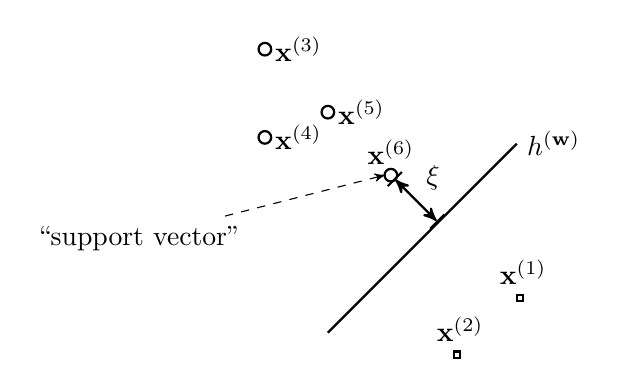
\begin{tikzpicture}[auto,scale=0.8]
%\draw [thick] (0,-3) rectangle (4,4) node [anchor=east,above] {$\featurespace$} ;
\draw [thick] (1,2) circle (0.1cm)node[anchor=west] {\hspace*{0mm}$\vx^{(5)}$};
\draw [thick] (0,1.6) circle (0.1cm)node[anchor=west] {\hspace*{0mm}$\vx^{(4)}$};
\draw [thick] (0,3) circle (0.1cm)node[anchor=west] {\hspace*{0mm}$\vx^{(3)}$};
\draw [thick] (2,1) circle (0.1cm)node[anchor=east,above] {\hspace*{0mm}$\vx^{(6)}$};
\node[] (B) at (-2,0) {``support vector''};
\draw[->,dashed] (B) to (1.9,1) ; 
\draw [|<->|,thick] (2.05,0.95)  -- (2.75,0.25)node[pos=0.5] {$\xi$} ; 
\draw [thick] (1,-1.5) -- (4,1.5) node [right] {$h^{(\vw)}$} ; 
\draw [thick] (3,-1.9) rectangle ++(0.1cm,0.1cm) node[anchor=west,above]  {\hspace*{0mm}$\vx^{(2)}$};
\draw [thick] (4,.-1) rectangle ++(0.1cm,0.1cm) node[anchor=west,above] {\hspace*{0mm}$\vx^{(1)}$};
\end{tikzpicture}
\caption{The SVM aims at a classifier $h^{(\vw)}$ with small hinge loss. 
	Minimizing hinge loss of a classifier is the same as maximizing the 
	margin $\xi$ between the decision boundary (of the classifier) and 
	each class of the training set.}
\label{fig_svm}
\end{center}
\end{figure}

We highlight that both, the SVM and logistic regression amount to linear 
classifiers $h^{(\vw)} \in \hypospace^{(\featuredim)}$ (see \eqref{equ_lin_hypospace}) 
whose decision boundary is a hyperplane in the feature space $\featurespace = \mathbb{R}^{\featuredim}$ (see Figure \ref{fig_lin_dec_boundary}). The difference between SVM and logistic regression is the loss function used for 
evaluating the quality of a particular classifier $h^{(\vw)} \in \hypospace^{(\featuredim)}$. 
The SVM uses the hinge loss \eqref{equ_hinge_loss} which is the best 
convex approximation to the $0/1$ loss \eqref{equ_def_0_1}. Thus, we 
expect the classifier obtained by the SVM to yield a smaller classification 
error probability $\prob{ \hat{y} \neq y }$ (with $\hat{y} =1$ if $h(\vx)\geq0$ and 
$\hat{y}=-1$ otherwise) compared to logistic regression which uses 
the logistic loss \eqref{equ_log_loss}. 

The statistical superiority of the SVM comes at the cost of increased 
computational complexity. In particular, the hinge loss \eqref{equ_hinge_loss} 
is non-differentiable which prevents the use of  simple gradient-based 
methods (see Chapter \ref{ch_GD}) and requires more advanced optimization 
methods. In contrast, the logistic loss \eqref{equ_log_loss} is convex and 
differentiable. We can therefore use gradient based methods to minimize 
the average logistic loss incurred on a training set (see Chapter \ref{ch_GD}). 


\section{Bayes' Classifier}
\label{sec_NaiveBayes}

Consider datapoints characterized by features $\vx \in \featurespace$ 
and some binary label $y \in \labelspace$. We can use any two different 
label values but let us assume that the two possible label values 
are $y=-1$ and $y=1$. 

%The family 
%of Bayes' classifier methods is based on ML problems using the $0/1$ 
%loss \eqref{equ_def_0_1} for assessing the quality of classifiers $h$. 

The goal of ML is to find (or learn) a classifier $h: \featurespace \rightarrow \labelspace$ 
such that the predicted (or estimated) label $\hat{y} = h(\vx)$ agrees 
with the true label $y \in \labelspace$ as much as possible. Thus, it 
is reasonable to assess the quality of a classifier $h$ using the $0/1$ 
loss \eqref{equ_def_0_1}. We could then learn a classifier using the ERM 
with the loss function \eqref{equ_def_0_1}. However, the resulting 
optimization problem is typically intractable since the loss \eqref{equ_def_0_1} 
is non-convex and non-differentiable. 

We take a different route to construct a classifier, which we refer to 
as Bayes' classifier. This construction is based on a simple probabilistic 
model for the datapoints. Using this model, we can interpret the average 
$0/1$ loss on training data as an approximation for the probability 
%with its features $\vx$ and label $y$, as i.i.d. 
%random variables, the $0/1$ loss approximates the misclassification (error) 
%probability  
$P_{\rm err} = \prob{ y \neq h(\vx) }$. 


An important subclass of Bayes' classifiers uses the hypothesis 
space \eqref{equ_lin_hypospace} which is also underlying logistic 
regression (see Section \ref{sec_LogReg}) and the SVM (see Section 
\ref{sec_SVM}). Logistic regression, the SVM and Bayes' 
classifiers are different instances of linear classifiers (see Figure \ref{fig_lin_dec_boundary}). 

Linear classifiers partition the feature space $\featurespace$ into two half-spaces. 
One half-space consists of all feature vectors $\vx$ which result in the 
predicted label $\hat{y}=1$ and the other half-space constituted by all 
feature vectors $\vx$ which result in the predicted label $\hat{y}=-1$. 
The difference between these three linear classifiers is how they choose 
these half-spaces by using different loss functions. We will discuss 
Bayes' classifier methods in more detail in Section \ref{sec_ERM_Bayes}.  

 
\section{Kernel Methods} 
\label{sec_kernel_methods}

Consider a ML (classification or regression) problem with an 
underlying feature space $\featurespace$. In order to predict 
the label $y \in \labelspace$ of a datapoint based on its 
features $\vx \in \featurespace$, we apply a predictor $h$ 
selected out of some hypothesis space $\hypospace$. Let 
us assume that the available computational infrastructure only 
allows to use a linear hypothesis space $\hypospace^{(\featuredim)}$ (see \eqref{equ_lin_hypospace}).

For some applications, using a linear hypothesis $h(\vx)=\vw^{T}\vx$ 
is not suitable since the relation between features $\vx$ and label $y$ 
might be highly non-linear. %(see Figure \ref{fig_scatterplot_poly} 
One approach to extend the capabilities of linear hypotheses 
is to transform the raw features of a data point before applying a 
linear hypothesis $h$. 

The family of kernel methods is based on transforming the 
features $\vx$ to new features $\hat{\vx} \in \featurespace'$ 
which belong to a (typically very) high-dimensional space $\featurespace'$ \cite{LampertNowKernel}. It is 
not uncommon that, while the original feature space is a 
low-dimensional Euclidean space (e.g., $\featurespace = \mathbb{R}^{2}$), 
the transformed feature space $\featurespace'$ is an infinite-dimensional function space. 

The rationale behind transforming the original features into a 
new (higher-dimensional) feature space $\featurespace'$ is to 
reshape the intrinsic geometry of the feature vectors 
$\vx^{(\sampleidx)} \in \featurespace$ such that the transformed 
feature vectors $\hat{\vx}^{(\sampleidx)}$ have a ``simpler'' 
geometry (see Figure \ref{fig_kernelmethods}). 

Kernel methods are obtained by formulating ML problems 
(such as linear regression or logistic regression) using the 
transformed features $\hat{\vx}= \phi(\vx)$. A key challenge 
within kernel methods is the choice of the feature map $\phi: \featurespace \rightarrow \featurespace'$ which 
maps the original feature vector $\vx$ to a new feature vector $\hat{\vx}= \phi(\vx)$. 


\begin{figure}[htbp]
\begin{center}
\begin{minipage}{0.45\textwidth}
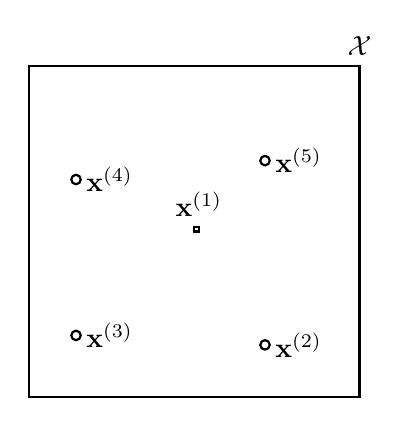
\begin{tikzpicture}[auto,scale=0.6]
\draw [thick] (-3,-3) rectangle (4,4) node [anchor=east,above] {$\featurespace$} ;
\draw [thick] (2,2) circle (0.1cm)node[anchor=west] {\hspace*{0mm}$\vx^{(5)}$};
\draw [thick] (-2,1.6) circle (0.1cm)node[anchor=west] {\hspace*{0mm}$\vx^{(4)}$};
\draw [thick] (-2,-1.7) circle (0.1cm)node[anchor=west] {\hspace*{0mm}$\vx^{(3)}$};
\draw [thick] (2,-1.9) circle (0.1cm) node[anchor=west] {\hspace*{0mm}$\vx^{(2)}$};
\draw [thick] (.5,.5) rectangle ++(0.1cm,0.1cm) node[anchor=west,above] {\hspace*{0mm}$\vx^{(1)}$};
 %       \node[] (B) at (12,2) {$\labelspace$};
  %       \fill  (11.5,2.5)  circle (2pt) node[above] (D) {$y \in \labelspace$};    
   %      \draw [->,thick] (5,3)   --  (11.5,2.5) node[above,midway] {$h(\vx)$} ;
\end{tikzpicture}
\end{minipage}
\begin{minipage}{0.45\textwidth}
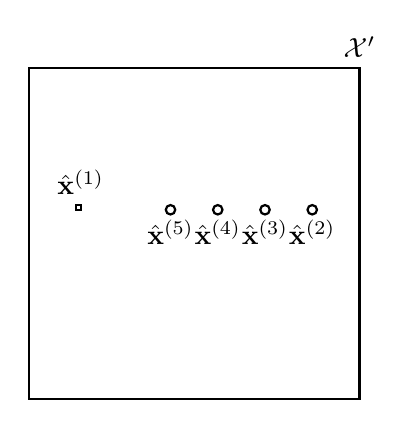
\begin{tikzpicture}[auto,scale=0.6]
\draw [thick] (0,-4) rectangle (7,3) node [anchor=east,above] {$\featurespace'$} ;
\draw [thick] (3,0) circle (0.1cm)node[anchor=north] {\hspace*{0mm}$\hat{\vx}^{(5)}$};
\draw [thick] (4,0) circle (0.1cm)node[anchor=north] {\hspace*{0mm}$\hat{\vx}^{(4)}$};
\draw [thick] (5,0) circle (0.1cm)node[anchor=north] {\hspace*{0mm}$\hat{\vx}^{(3)}$};
\draw [thick] (6,0) circle (0.1cm) node[anchor=north] {\hspace*{0mm}$\hat{\vx}^{(2)}$};
\draw [thick] (1,0) rectangle ++(0.1cm,0.1cm) node[anchor=west,above] {\hspace*{0mm}$\hat{\vx}^{(1)}$};
 %       \node[] (B) at (12,2) {$\labelspace$};
  %       \fill  (11.5,2.5)  circle (2pt) node[above] (D) {$y \in \labelspace$};    
   %      \draw [->,thick] (5,3)   --  (11.5,2.5) node[above,midway] {$h(\vx)$} ;
   \end{tikzpicture}
\end{minipage}
\caption{Consider a data set $\dataset = \{ (\vx^{(\sampleidx)},y^{(\sampleidx)}) \}_{\sampleidx=1}^{5}$ constituted 
by datapoints with features $\vx^{(\sampleidx)}$ and binary labels $y^{(\sampleidx)}$. Left: In the original feature 
space $\featurespace$, the datapoints cannot be separated perfectly by any linear classifier. Right: The feature 
map $\phi: \featurespace \rightarrow \featurespace'$ transforms the features $\vx^{(\sampleidx)}$ to the new features 
$\hat{\vx}^{(\sampleidx)}=\phi\big(\vx^{(\sampleidx)}\big)$ in the new feature space $\featurespace'$. In the new 
feature space $\featurespace'$ the datapoints can be separated perfectly by a linear classifier. }
\label{fig_kernelmethods}
\end{center}
\end{figure}


\newpage
\section{Decision Trees} 
\label{sec_decision_trees}

A decision tree is a flowchart-like description of a map 
$h: \featurespace \rightarrow \labelspace$ which maps 
the features $\vx \in \featurespace$ of a datapoint to a 
predicted label $h(\vx) \in \labelspace$ \cite{hastie01statisticallearning}. 

While decision trees can be used for arbitrary feature space 
$\featurespace$ and label space $\labelspace$, we will discuss 
them for the particular feature space $\featurespace = \mathbb{R}^{2}$ 
and label space $\labelspace=\mathbb{R}$. %Here, a decision tree describes 
%how a feature vector $\vx=(x_{1},x_{2})^{T}$ is mapped to a predicted label $h(\vx)$. 

We have depicted an example of a decision tree in Figure \ref{fig_decision_tree}. 
The decision tree consists of nodes which are connected by directed edges. 
We might think of a decision tree as a step-by-step instruction, 
or a ``recipe'', for how to compute the function value $h(\vx)$ 
given the features $\vx \in \featurespace$ of a datapoint. This 
computation starts at the {\bf root node} and ends at one of 
the {\bf leaf nodes} of the decision tree. 

A leaf node $m$, which does not have any outgoing edges, 
represents a decision region $\mathcal{R}_{m} \subseteq \featurespace$ in 
the feature space. The hypothesis $h$ associated with a decision tree 
is constant over the regions $\mathcal{R}_{m}$, such that $h(\vx) = h_{m}$ 
for all $\vx \in \mathcal{R}_{m}$ and some fixed number $h_{m} \in \mathbb{R}$. 

In general, there are two types of nodes in a decision tree: 
\begin{itemize} 
\item decision (or test) nodes, which represent particular ``tests'' 
about the feature vector $\vx$ (e.g., ``is the norm of $\vx$ larger than $10$?'').
\item leaf nodes, which correspond to subsets of the feature space. 
\end{itemize} 
The particular decision tree depicted in Figure \ref{fig_decision_tree} consists 
of two decision nodes (including the root node) and three leaf nodes. 

Given limited computational resources, we can only use decision 
trees which are not too deep. Consider the hypothesis space consisting 
of all decision trees which uses the tests ``$\| \vx - \vu \| \leq r$'' and  
``$\| \vx - \vv \| \leq r$'' , with some vectors $\vu$ and $\vv$, some positive 
radius $r >0$ and depth no larger than $2$.\footnote{The depth of a decision tree 
	is the maximum number of hops it takes to reach a leaf node starting 
	from the root and following the arrows. The decision tree depicted in Figure \ref{fig_decision_tree} has depth $2$.} 

To assess the quality of different decision trees we need to use some 
loss function. Examples of loss functions used to measure the quality 
of a decision tree are the squared error loss (for numeric labels) or the 
impurity of individual decision regressions (for discrete labels). 

In general, we are not interested in one particular decision tree only but 
in a large set of different decision trees from which we choose the most 
suitable given some data (see Section \ref{sec_ERM_decision_tree}). We 
can define a hypothesis space by collecting predictor maps $h$ represented 
by a set of decision trees (such as depicted in Figure \ref{fig_hypospace_DT_depth_2}). 

A collection of decision trees can be constructed based on a fixed set of 
``elementary tests'' on the input feature vector, e.g., $\| \vx \| > 3$, $x_{3} < 1$ 
or a continuous ensemble of parametrized tests such as $\{ x_{2} > \eta \}_ {\eta \in [0,10]}$. 
We then build a hypothesis space by considering all decision trees not 
exceeding a maximum depth and whose decision nodes carry out 
elementary tests. 

\begin{figure}[htbp]
\begin{minipage}{.45\textwidth} %
\scalebox{0.6}{
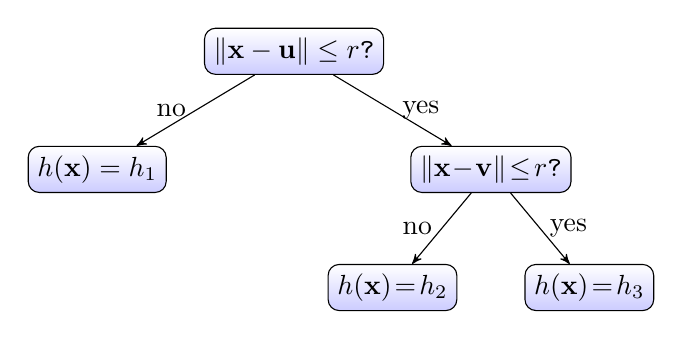
\begin{tikzpicture}
%  [scale=0.9, 
%    grow                    = right,
%    sibling distance        = 6em,
%    level distance          = 10em,
%    edge from parent/.style = {draw, -latex},
%    every node/.style       = {font=\footnotesize},
%    sloped
 % ]
  [->,>=stealth',level/.style={sibling distance = 5cm/#1,
   level distance = 1.5cm}] 
  \node [env] {$\| \vx-\vu \| \leq r$?}
    child { node [env] {$h(\vx) = h_{1} $}
      edge from parent node [left,align=center] {no} }
    child { node [env] {$\| \vx\!-\!\vv \|\!\leq\!r$?}
         child { node [env] {$h(\vx)\!=\!h_{2}$}
              edge from parent node [left, align=center] {no} }
         child { node [env] {$h(\vx)\!=\!h_{3}$}
              edge from parent node [right, align=center]
                {yes} }
     edge from parent node [right,align=center] {yes} };
\end{tikzpicture}
}
\end{minipage}
\begin{minipage}{.45\textwidth} %
\hspace*{15mm}
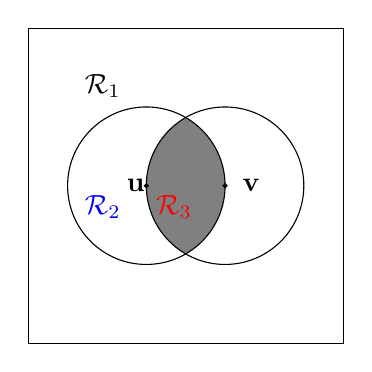
\begin{tikzpicture}
      \draw (-2,2) rectangle (2,-2);
      \begin{scope}
         \clip (-0.5,0) circle (1cm);
         \clip (0.5,0) circle (1cm);
         \fill[color=gray] (-2,1.5) rectangle (2,-1.5);
      \end{scope}
      \draw (-0.5,0) circle (1cm);
      \draw (0.5,0) circle (1cm);
               \draw[fill] (-0.5,0) circle [radius=0.025];
         \node [below right, red] at (-0.5,0) {$\mathcal{R}_{3}$};
                  \node [below left, blue] at (-0.7,0) {$\mathcal{R}_{2}$};
                    \node [above left] at (-0.7,1) {$\mathcal{R}_{1}$};
                  \node [left] at (-0.4,0) {$\mathbf{u}$};
                     \draw[fill] (0.5,0) circle [radius=0.025];
                     \node [right] at (0.6,0) {$\mathbf{v}$};
   \end{tikzpicture}
\end{minipage}
\caption{A decision tree represents a hypothesis $h$ which is constant on subsets $\mathcal{R}_{m}$, i.e., 
$h(\vx)\!=\!h_{m}$ for all $\vx\!\in\!\mathcal{R}_{m}$. Each subset 
$\mathcal{R}_{m}\!\subseteq\!\featurespace$ corresponds to a leaf node in the decision tree.}
\label{fig_decision_tree}
\end{figure} 

\begin{figure}[htbp]
\begin{center}
\begin{minipage}{.4\textwidth}
\scalebox{0.8}{
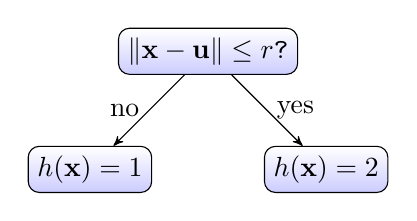
\begin{tikzpicture} [->,>=stealth',level/.style={sibling distance = 3cm/#1,
   level distance = 1.5cm}] 
\node [env] {$\| \vx-\vu \| \leq r$?}
child {node [env] {$h(\vx)=1$}
  edge from parent node [left,align=center] {no} }
child {node [env] {$h(\vx)=2$}
  edge from parent node [right,align=center] {yes} };
\end{tikzpicture}}
\end{minipage}
\hspace*{3mm}
\begin{minipage}{.4\textwidth}
\scalebox{0.8}{
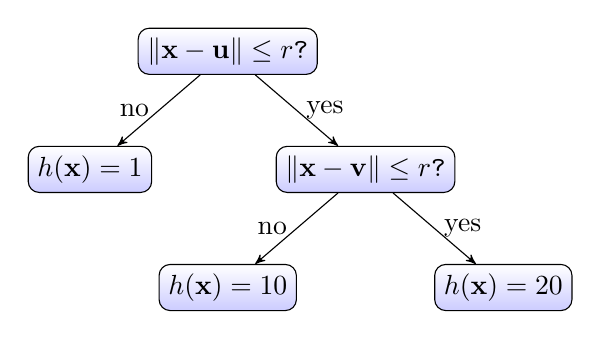
\begin{tikzpicture} [->,>=stealth',level/.style={sibling distance = 3.5cm,
   level distance = 1.5cm}] 
\node [env] {$\| \vx-\vu \| \leq r$?}
child {node [env] {$h(\vx)=1$}
  edge from parent node [left,align=center] {no} }
child {node  [env] {$\| \vx-\vv \| \leq r$?}    child {node  [env] {$h(\vx) =10$} edge from parent node [left,align=center] {no} }
   child {node  [env] {$h(\vx) =20$} edge from parent node [right,align=center] {yes} }
 edge from parent node [right,align=center] {yes} 
 };
\end{tikzpicture}}
      \end{minipage}
 \end{center}
 \caption{A hypothesis space $\hypospace$ consisting of two decision trees 
 	with depth at most $2$ and using the tests $\| \vx\!-\!\vu \|\!\leq\!r$ and $\|\vx\!-\!\vv \|\!\leq\!r$ 
 	with a fixed radius $r$ and vectors $\vu,\vv \in \mathbb{R}^{\featurelen}$. }
 \label{fig_hypospace_DT_depth_2}
\end{figure}

A decision tree represents a map $h: \featurespace \rightarrow \labelspace$, which 
is piecewise-constant over regions of the feature space $\featurespace$. These 
non-overlapping regions form a partitioning of the feature space. Each leaf node of 
a decision tree corresponds to one particular region. Using large decision trees, which 
involve many different test nodes, we can represent very complicated partitions 
that resemble any given labeled dataset (see Figure \ref{fig_decisiontree_overfits}). 

This is quite different from ML methods using the linear hypothesis space \eqref{equ_lin_hypospace}, 
such as linear regression, logistic regression or SVM. Such linear maps have a rather 
simple geometry. Indeed, a linear map is constant along hyperplanes. Moreover, the 
decision regions obtained from linear classifiers are always entire half-spaces (see Figure \ref{fig_lin_dec_boundary}). 

In contrast, the shape of a map represented by a decision tree can be highly 
complicated. Using a sufficiently large (deep) decision tree, we can obtain a 
map that closely resembles almost any given non-linear map. The decision 
regions obtained from a deep decision tree can be highly irregular. 

%can be arbitrary complicated if the decision tree is sufficiently large (deep). % we can construct a sufficiently complex 
%decision tree which partitions the feature space such that each datapoint belongs to a separate cluster (corresponding to a particular leaf node). 

\begin{figure}[htbp]
\begin{minipage}{0.4\textwidth}
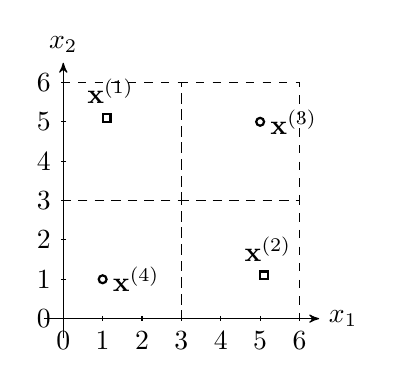
\begin{tikzpicture}[auto,scale=0.5]
%\draw [thick] (-3,-3) rectangle (1,4) node [anchor=east,above] {$\featurespace$} ;
\draw [thick] (5,5) circle (0.1cm)node[anchor=west] {\hspace*{0mm}$\vx^{(3)}$};
\draw [dashed] (3,3) rectangle (6,6) ;
\draw [dashed] (3,0) rectangle (6,3) ;
\draw [dashed] (0,3) rectangle (3,6) ;
\draw [dashed] (0,0) rectangle (3,3) ;
\draw [thick] (1,1) circle (0.1cm)node[anchor=west] {\hspace*{0mm}$\vx^{(4)}$};
%\draw [thick] (-2,-1.7) circle (0.1cm)node[anchor=west] {\hspace*{0mm}$\vx^{(3)}$};
%\draw [thick] (2,-1.9) circle (0.1cm) node[anchor=west] {\hspace*{0mm}$\vx^{(2)}$};
\draw [thick] (5,1) rectangle ++(0.2cm,0.2cm) node[anchor=west,above] {\hspace*{0mm}$\vx^{(2)}$};
\draw [thick] (1,5) rectangle ++(0.2cm,0.2cm) node[anchor=west,above] {\hspace*{0mm}$\vx^{(1)}$};
\draw[->] (-0.5,0) -- (6.5,0) node[right] {$x_{1}$};
\draw[->] (0,-0.5) -- (0,6.5) node[above] {$x_{2}$};
\foreach \y/\ytext in {0/0, 1/1,2/2,3/3,4/4,5/5,6/6} \draw[shift={(0,\y)}] (2pt,0pt) -- (-2pt,0pt) node[left] {$\ytext$};  
\foreach \x/\xtext in{0/0, 1/1,2/2,3/3,4/4,5/5,6/6}\draw[shift={(\x,0)}] (0pt,2pt) -- (0pt,-2pt) node[below] {$\xtext$};  
 %       \node[] (B) at (12,2) {$\labelspace$};
  %       \fill  (11.5,2.5)  circle (2pt) node[above] (D) {$y \in \labelspace$};    
   %      \draw [->,thick] (5,3)   --  (11.5,2.5) node[above,midway] {$h(\vx)$} ;
\end{tikzpicture}
\end{minipage}
%\hspace*{-10mm}
\begin{minipage}{0.44\textwidth}
\scalebox{0.6}{
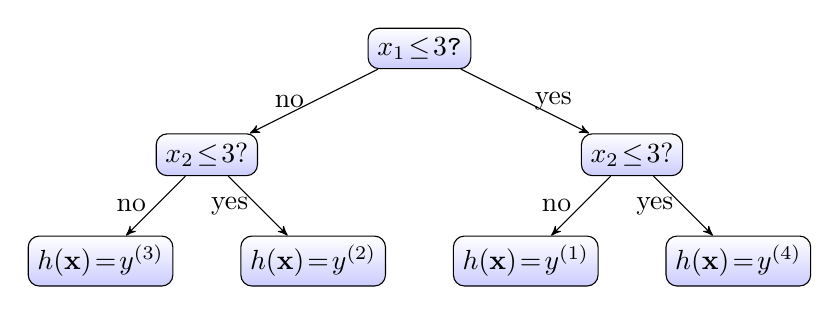
\begin{tikzpicture} [->,>=stealth',level/.style={sibling distance = 3cm/#1,
   level distance = 1.5cm},scale=0.9] 
\tikzstyle{level 1}=[sibling distance=60mm]
  \tikzstyle{level 2}=[sibling distance=30mm]
\node [env] {$x_{1}\!\leq\!3$?}
child  {node [env] {$x_{2}\!\leq\!3?$} 
    child {node [env] {$h(\vx)\!=\!y^{(3)}$}  edge from parent node [left,align=center] {no}}
    child {node [env] {$h(\vx)\!=\!y^{(2)}$}   edge from parent node [left,align=center] {yes}}
  edge from parent node [left,align=center] {no} }
child { node [env]  {$x_{2}\!\leq\!3?$}
   child {node [env] {$h(\vx)\!=\!y^{(1)}$}   edge from parent node [left,align=center] {no} }
    child {node [env] {$h(\vx)\!=\!y^{(4)}$}   edge from parent node [left,align=center] {yes} }
  edge from parent node [right,align=center] {yes}};
\end{tikzpicture}}
\end{minipage}
\caption{Using a sufficiently large (deep) decision tree, we can construct a map $h$ that perfectly fits any given 
labeled dataset $\{(\vx^{(\sampleidx)},y^{(\sampleidx)} ) \}_{\sampleidx=1}^{\samplesize}$ such that 
$h(\vx^{(\sampleidx)})\!=\!y^{(\sampleidx)}$ for $\sampleidx=1,\ldots,\samplesize$.}
\label{fig_decisiontree_overfits}
\end{figure}



\newpage
\section{Artificial Neural Networks -- Deep Learning} 
\label{sec_deep_learning}

Another example of a hypothesis space, which has proven useful 
in a wide range of applications, e.g., image captioning or automated 
translation,  is based on a {\bf network representation} of a predictor 
$h: \mathbb{R}^{\featuredim} \rightarrow \mathbb{R}$. We can define 
a predictor  $h^{(\vw)}: \mathbb{R}^{\featuredim} \rightarrow \mathbb{R}$ 
using an {\bf artificial neural network} (ANN) structure as depicted in Figure \ref{fig_ANN}. 
\begin{figure}[htbp]
\centering
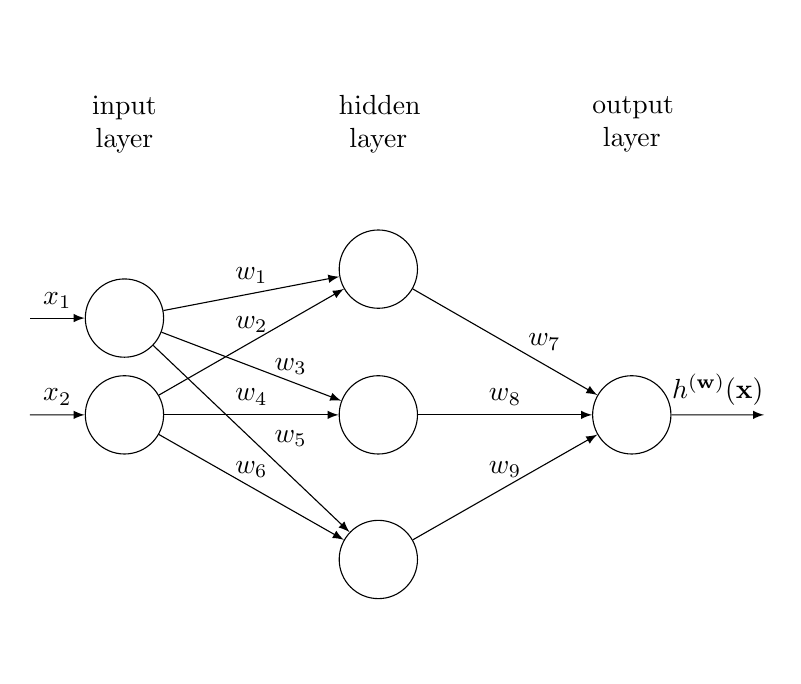
\begin{tikzpicture}[
plain/.style={
  draw=none,
  fill=none,
  },
net/.style={
  matrix of nodes,
  nodes={
    draw,
    circle,
    inner sep=10pt
    },
  nodes in empty cells,
  column sep=1cm,
  row sep=-11pt
  },
>=latex, 
scale=0.6
]
\matrix[net] (mat)
{
|[plain]| \parbox{1cm}{\centering input\\layer} & |[plain]| \parbox{1cm}{\centering hidden\\layer} & |[plain]| \parbox{1cm}{\centering output\\layer} \\
|[plain]|&  |[plain]|\\
|[plain]| & \\
& |[plain]| \\
  |[plain]| & |[plain]| \\
& & \\
  |[plain]| & |[plain]| \\
|[plain]| & |[plain]| \\
  |[plain]| & \\
|[plain]| & |[plain]| \\    };
 \draw[<-] (mat-4-1) -- node[above] {$x_{1}$} +(-2cm,0);
  \draw[<-] (mat-6-1) -- node[above] {$x_{2}$} +(-2cm,0);
    \draw[->] (mat-4-1) --  node[above]{$w_{1}$}  (mat-3-2);
      \draw[->] (mat-6-1) --  node[above]{$w_{2}$}  (mat-3-2);
        \draw[->] (mat-4-1) --  node[]{\hspace*{10mm}$w_{3}$}  (mat-6-2);
      \draw[->] (mat-6-1) --  node[above]{$w_{4}$}  (mat-6-2);
              \draw[->] (mat-4-1) --  node[]{\hspace*{10mm}$w_{5}$}  (mat-9-2);
      \draw[->] (mat-6-1) --  node[above]{$w_{6}$}  (mat-9-2);
       \draw[->] (mat-3-2) --  node[]{\hspace*{10mm}$w_{7}$}  (mat-6-3);
      \draw[->] (mat-6-2) --  node[above]{$w_{8}$}  (mat-6-3);
      \draw[->] (mat-9-2) --  node[above]{$w_{9}$}  (mat-6-3);     
      \draw[->] (mat-6-3) -- node[above] {$h^{(\vw)}(\vx)$} +(2.8cm,0);
  \vspace*{-4mm}
\end{tikzpicture}
  \vspace*{-4mm}
\caption{ANN representation of a predictor $h^{(\vw)}(\vx)$ which maps 
	the input (feature) vector $\vx=(x_{1},x_{2})^{T}$ to a predicted label (output) $h^{(\vw)}(\vx)$.}
    \label{fig_ANN}
\end{figure}
A feature vector $\vx \in \mathbb{R}^{\featuredim}$ is fed into the input units, 
each of which reads in one single feature $x_{i} \in \mathbb{R}$. The features 
$x_{i}$ are then multiplied with the weights $w_{j,i}$ associated with the link 
between the $\sampleidx$-th input node (``neuron'') with the $j$-th node 
in the middle (hidden) layer. The output of the $j$-th node in the hidden layer 
is given by $s_{j} = g( \sum_{i=1}^{\featuredim} w_{j,i} x_{i} )$ with some 
(typically non-linear) {\bf activation function} $g(z)$. The input (or activation) 
$z$ for the activation (or output) $g(z)$ of a neuron is a weighted 
(linear) combination $ \sum_{i=1}^{\featuredim} w_{j,i} s_{i}$ of the outputs $s_{i}$ 
of the nodes in the previous layer. For the ANN depicted in Figure \ref{fig_ANN}, 
the activation of the neuron $s_{1}$ is $z=w_{1,1}x_{1} + w_{1,2}x_{2}$.

Two popular choices for the activation function used within ANNs 
are the {\bf sigmoid function} $g(z) = \frac{1}{1+\exp(-z)}$ or the 
{\bf rectified linear unit} $g(z) = \max\{0,z\}$. An ANN with many, 
say $10$, hidden layers, is often referred to as a {\bf deep neural network} 
and the obtained ML methods are known as {\bf deep learning} methods (see \cite{Goodfellow-et-al-2016} for an in-depth 
introduction to deep learning methods). 

Remarkably, using some simple non-linear activation function $g(z)$ as the building 
block for ANNs allows to represent an extremely large class of predictor maps 
$h^{(\vw)}: \mathbb{R}^{\featuredim} \rightarrow \mathbb{R}$. The hypothesis 
space generated by a given ANN structure, i.e., the set of all predictor maps which 
can be implemented by a given ANN and suitable weights $\vw$, tends to be 
much larger than the hypothesis space \eqref{equ_def_hypo_linear_pred} of 
linear predictors using weight vectors $\vw$ of the same length \cite[Ch. 6.4.1.]{Goodfellow-et-al-2016}. 
It can be shown that an ANN with only one single hidden layer can approximate any given map $h: \featurespace \rightarrow \labelspace=\mathbb{R}$ 
to any desired accuracy \cite{Cybenko1989}. However, a key insight which underlies many 
deep learning methods is that using several layers with few neurons, instead of one 
single layer containing many neurons, is computationally favourable \cite{DBLP:journals/corr/EldanS15}. 
\begin{center}
\begin{figure}[htbp]
	\centering
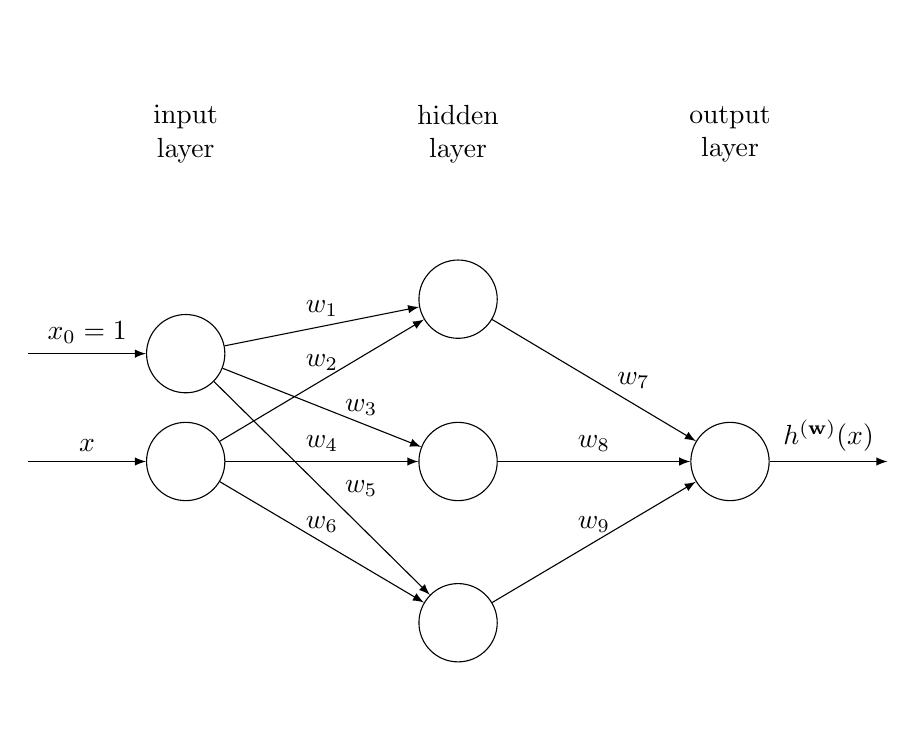
\begin{tikzpicture}[
plain/.style={
  draw=none,
  fill=none,
  },
net/.style={
  matrix of nodes,
  nodes={
    draw,
    circle,
    inner sep=10pt
    },
  nodes in empty cells,
  column sep=1cm,
  row sep=-9pt
  },
>=latex
]
\matrix[net] (mat)
{
|[plain]| \parbox{1.3cm}{\centering input\\layer} & |[plain]| \parbox{1.3cm}{\centering hidden\\layer} & |[plain]| \parbox{1.3cm}{\centering output\\layer} \\
|[plain]|&  |[plain]|\\
|[plain]| & \\
& |[plain]| \\
  |[plain]| & |[plain]| \\
& & \\
  |[plain]| & |[plain]| \\
|[plain]| & |[plain]| \\
  |[plain]| & \\
|[plain]| & |[plain]| \\    };
 \draw[<-] (mat-4-1) -- node[above] {$x_{0}=1$} +(-2cm,0);
  \draw[<-] (mat-6-1) -- node[above] {$x$} +(-2cm,0);
    \draw[->] (mat-4-1) --  node[above]{$w_{1}$}  (mat-3-2);
      \draw[->] (mat-6-1) --  node[above]{$w_{2}$}  (mat-3-2);
        \draw[->] (mat-4-1) --  node[]{\hspace*{10mm}$w_{3}$}  (mat-6-2);
      \draw[->] (mat-6-1) --  node[above]{$w_{4}$}  (mat-6-2);
              \draw[->] (mat-4-1) --  node[]{\hspace*{10mm}$w_{5}$}  (mat-9-2);
      \draw[->] (mat-6-1) --  node[above]{$w_{6}$}  (mat-9-2);
       \draw[->] (mat-3-2) --  node[]{\hspace*{10mm}$w_{7}$}  (mat-6-3);
      \draw[->] (mat-6-2) --  node[above]{$w_{8}$}  (mat-6-3);
      \draw[->] (mat-9-2) --  node[above]{$w_{9}$}  (mat-6-3);     
      \draw[->] (mat-6-3) -- node[above] {$h^{(\vw)}(x)$} +(2cm,0);
\end{tikzpicture}
\caption{This ANN with one hidden layer defines a hypothesis space consisting of all maps $h^{(\vw)}(x)$ obtained 
by implementing the ANN with different weight vectors $\vw = (w_{1},\ldots,w_{9})^{T}$.} 
\label{fig_a_ANN}
\end{figure}
\end{center}

\begin{figure}[htbp]
\centering
\begin{tikzpicture}[
plain/.style={
  draw=none,
  fill=none,
  },
net/.style={
  matrix of nodes,
  nodes={
    draw,
    circle,
    inner sep=10pt
    },
  nodes in empty cells,
  column sep=2cm,
  row sep=-9pt
  },
>=latex
]
\matrix[net] (mat)
{
|[plain]| &|[plain]| \\
|[plain]|& |[plain]| \\
  |[plain]| & |[plain]| \\
|[plain]|& & |[plain]|\\
|[plain]|& |[plain]| \\
|[plain]| & |[plain]| \\
  |[plain]| &|[plain]| \\  };
% \draw[<-] (mat-4-1) -- node[above] {$x_{0}=1$} +(-2cm,0);
%  \draw[<-] (mat-6-1) -- node[above] {$x$} +(-2cm,0);
   \draw[->] (mat-2-1) node[]{$x_{1}$} --  node[above]{$w_{1}$}  (mat-4-2);
%      \draw[->] (mat-6-1) --  node[above]{$w_{2}$}  (mat-3-2);
        \draw[->] (mat-4-1) node[]{$x_{2}$}  --  node[above]{$w_{2}$}  (mat-4-2) ;
      \draw[->] (mat-6-1) node[]{$x_{3}$}--  node[above]{$w_{3}$}  (mat-4-2);
           %   \draw[->] (mat-4-1) --  node[]{\hspace*{10mm}$w_{5}$}  (mat-9-2);
     % \draw[->] (mat-6-1) --  node[above]{$w_{6}$}  (mat-9-2);
  %     \draw[->] (mat-3-2) --  node[]{\hspace*{10mm}$w_{7}$}  (mat-6-3);
   %   \draw[->] (mat-6-2) --  node[above]{$w_{8}$}  (mat-6-3);
    %  \draw[->] (mat-9-2) --  node[above]{$w_{9}$}  (mat-6-3);     
      \draw[->] (mat-4-2) -- node[above] {$g(z)$} +(2cm,0);
\end{tikzpicture}
\caption{Each single neuron of the ANN depicted in Figure \ref{fig_a_ANN} implements 
	a weighted summation $z=\sum_{i} w_{i} x_{i}$ of its inputs $x_{i}$ followed by applying 
	a non-linear activation function $g(z)$.}
\label{fig_activate_neuron}
\end{figure}

\begin{center}
\framebox[0.96\textwidth]{
 \parbox{0.9\textwidth}{
{\bf Exercise.} Consider the simple ANN structure in Figure \ref{fig_a_ANN} using the 
``ReLu'' activation function $g(z)= \max\{z,0\}$ (see Figure \ref{fig_activate_neuron}). Show 
that there is a particular choice for the weights $\vw =(w_{1},\ldots,w_{9})^{T}$ 
such that the resulting hypothesis map $h^{(\vw)}(x)$ is a triangle as depicted in 
Figure \ref{fig_triangle}. Can you also find a choice for the weights $\vw =(w_{1},\ldots,w_{9})^{T}$ 
that produce the same triangle shape if we replace the ReLu activation function 
with the linear function $g(z) =10 \cdot z$?
}}
\end{center}


\begin{figure}[htbp]
\begin{center}
    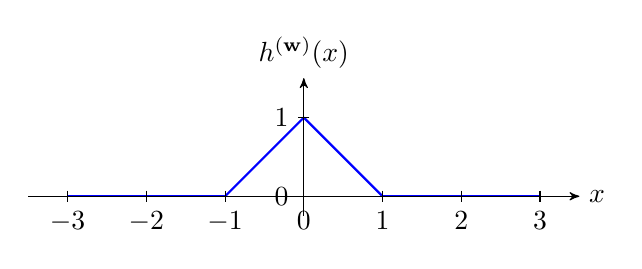
\begin{tikzpicture}
       %   \begin{axis}
       %   [ylabel=$h(x)$,
         %     xlabel=$x$,grid]
             %  \addplot table [x=a, y=b, col sep=comma] {data.csv};      
                 \draw[blue,  thick, domain=-3:-1] plot (\x,  {0*\x});
                 \draw[blue,  thick, domain=-1:0] plot (\x,  {1+\x}); 
                 \draw[blue,  thick, domain=0:1] plot (\x,  {1-\x});    
                   \draw[blue,  thick, domain=1:3] plot (\x,  {0});           
          \draw[->] (-3.5,0) -- (3.5,0) node[right] {$x$};
   \draw[->] (0,-0.25) -- (0,1.5) node[above] {$h^{(\vw)}(x)$};
           %      \draw[dashed, thick, domain=1:3.6] plot (\x,  {\x - 1}) node[right] {$ f(\vw_{0})\!+\!(\vw\!-\!\vw_{0})^{T} \nabla f(\vw_{0})$};
                    \foreach \y/\ytext in {0/0, 1/1}
    \draw[shift={(0,\y)}] (2pt,0pt) -- (-2pt,0pt) node[left] {$\ytext$};  
                        \foreach \x/\xtext in {-3/-3,-2/-2,-1/-1,0/0,1/1, 2/2,3/3}
    \draw[shift={(\x,0)}] (0pt,2pt) -- (0pt,-2pt) node[below] {$\xtext$};  
       %   \end{axis}
     \end{tikzpicture}
     \vspace*{-10mm}
\end{center}
\caption{A hypothesis map with the shape of a triangle.}
\label{fig_triangle}
\end{figure}

The recent success of ML methods based on ANN with many hidden layers 
(which makes them deep) might be attributed to the fact that the network 
representation of hypothesis maps is beneficial for the computational 
implementation of ML methods. First, we can evaluate a map $h^{(\vw)}$ represented 
by an ANN efficiently using modern parallel and distributed computing 
infrastructure via message passing over the network. Second, the 
graphical representation of a parametrized hypothesis in the form 
of a ANN allows to efficiently compute the gradient of the loss function via a message passing 
procedure known as {\bf back-propagation} \cite{Goodfellow-et-al-2016}.

\section{Maximum Likelihood Methods}
\label{sec_max_iikelihood}

For many applications it is useful to model the observed datapoints $\vz^{(\sampleidx)}$ 
as realizations of a random variable $\vz$ with probability distribution $\prob{\vz; \mathbf{w}}$ 
which depends on some parameter vector $\vw \in \mathbb{R}^{\featuredim}$. A principled 
approach to estimating the vector $\vw$ based on several independent and identically 
distributed (i.i.d.) realizations $\vz^{(1)},\ldots,\vz^{(\samplesize)}\sim \prob{\vz; \mathbf{w}}$ is 
{\bf maximum likelihood estimation} \cite{LC}. 

Maximum likelihood estimation can be interpreted as an ML problem with a hypothesis space 
parameterized by the weight vector $\vw$, i.e., each element $h^{(\vw)}$ of the hypothesis 
space $\hypospace$ corresponds to one particular choice for the 
weight vector $\vw$, and the loss function 
\begin{equation} 
\label{equ_loss_ML}
\loss{\vz}{h^{(\vw)}} \defeq - \log {\rm P} (\vz; \vw). 
\end{equation} 

A widely used choice for the probability distribution $\prob{\vz; \mathbf{w}}$ is a multivariate normal 
distribution with mean ${\bm \mu}$ and covariance matrix ${\bf \Sigma}$, both of which constitute the 
weight vector $\vw = ({\bm \mu}, {\bf \Sigma})$ (we have to reshape the matrix ${\bf \Sigma}$ suitably 
into a vector form). Given the i.i.d.\ realizations $\vz^{(1)},\ldots,\vz^{(\samplesize)} \sim \prob{\vz; \mathbf{w}}$,  
the maximum likelihood estimates $\hat{\bm \mu}$, $\widehat{\bf \Sigma}$ of the mean vector and 
the covariance matrix are obtained via 
\begin{equation}
\label{equ_max_likeli}
\hat{\bm \mu}, \widehat{\bf \Sigma} = \argmin_{{\bm \mu} \in \mathbb{R}^{\featurelen},{\bf \Sigma} \in \mathbb{S}^{\featurelen}_{+}} (1/\samplesize) \sum_{\sampleidx=1}^{\samplesize} - \log {\rm P} (\vz^{(\sampleidx)}; ({\bm \mu},{\bf \Sigma})). 
\end{equation} 

The optimization in \eqref{equ_max_likeli} is over choices for the mean 
vector ${\bm \mu} \in \mathbb{R}^{\featurelen}$ and covariance matrix 
${\bf \Sigma} \in \mathbb{S}^{\featurelen}_{+}$. Here, $\mathbb{S}^{\featurelen}_{+}$ 
denotes the set of all psd Hermitian $\featurelen \times \featurelen$ matrices. 

The maximum likelihood problem \eqref{equ_max_likeli} can be 
interpreted as an instance of ERM \eqref{equ_def_ERM_funs} using the 
particular loss function \eqref{equ_loss_ML}. The resulting estimates are 
given explicitly as 
\begin{equation}
\label{equ_ML_mean_cov_Gauss} 
\hat{\bm \mu} = (1/\samplesize) \sum_{\sampleidx=1}^{\samplesize} \vz^{(\sampleidx)} \mbox{, and } \widehat{\bf \Sigma} = (1/\samplesize) \sum_{\sampleidx=1}^{\samplesize} (\vz^{(\sampleidx)} - \hat{\bm \mu})(\vz^{(\sampleidx)} - \hat{\bm \mu})^{T}.
\end{equation} 

Note that the expressions \eqref{equ_ML_mean_cov_Gauss} 
are valid only when the probability distribution of the datapoints is 
modelled as a multivariate normal distribution. 

\section{Nearest Neighbour Methods} 
The class of $k$-nearest neighbour (k-NN) predictors (for continuous label space) or 
classifiers (for discrete label space) is defined for feature spaces $\featurespace$ equipped 
with an intrinsic notion of distance between its elements. Mathematically, such spaces are 
referred to as metric spaces \cite{RudinBookPrinciplesMatheAnalysis}. A prime example of a 
metric space is $\mathbb{R}^{\featuredim}$ with the Euclidean metric induced by the distance 
measure $\| \vx\!-\!\vy \|$ between two vectors $\vx, \vy \in \mathbb{R}^{\featuredim}$. 

The hypothesis space underlying $k$-NN problems consists of all maps $h: \featurespace \rightarrow \labelspace$ 
such that the function value $h(\vx)$ for a particular feature vector $\vx$ depends only on the (labels of the) $k$ 
nearest datapoints of some labeled training data $\dataset = \{ (\vx^{(\sampleidx)},y^{(\sampleidx)}) \}_{\sampleidx=1}^{\samplesize}$. 

In contrast to the ML problems discussed above in Section \ref{sec_lin_regression} - Section \ref{sec_deep_learning}, 
the hypothesis space of $k$-NN depends on the training data $\dataset$. 
\begin{figure}[htbp]
    \centering
 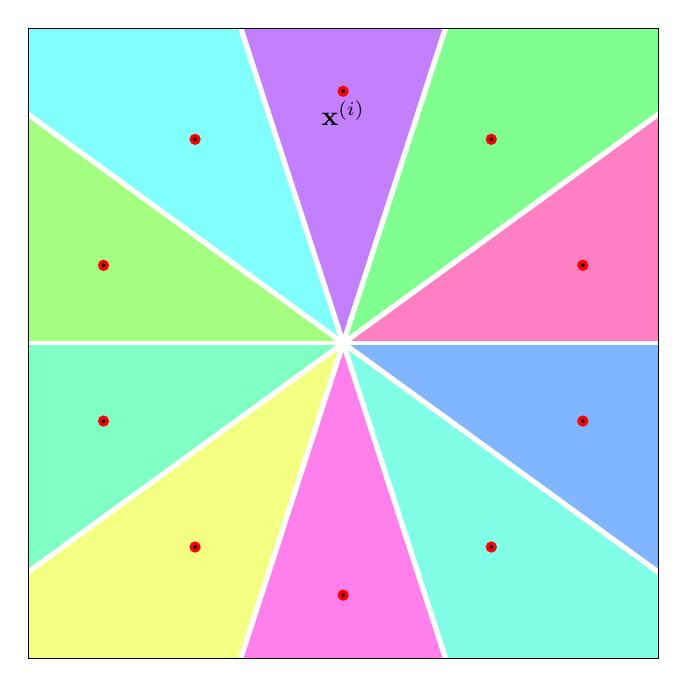
\begin{tikzpicture}
    % generate random points
    \pgfmathsetseed{1908} % init random with the year Voronoi published his paper ;)
    \def\pts{}
    \xintFor* #1 in {\xintSeq {1}{10}} \do{
  %    \pgfmathsetmacro{\ptx}{.9*\maxxy*rand} % random x in [-.9\maxxy,.9\maxxy]
    %  \pgfmathsetmacro{\pty}{.9*\maxxy*rand} % random y in [-.9\maxxy,.9\maxxy]
      \pgfmathsetmacro{\ptx}{0.8*\maxxy*sin(#1 * 36 )} % random x in [-.9\maxxy,.9\maxxy]
      \pgfmathsetmacro{\pty}{0.8*\maxxy*cos(#1 * 36 )} % random y in [-.9\maxxy,.9\maxxy]
    
      \edef\pts{\pts, (\ptx,\pty)} % stock the random point
    }
    % draw the points and their cells
    \xintForpair #1#2 in \pts \do{
      \edef\pta{#1,#2}
      \begin{scope}
        \xintForpair \#3#4 in \pts \do{
          \edef\ptb{#3,#4}
          \ifx\pta\ptb\relax % check if (#1,#2) == (#3,#4) ?
            \tikzstyle{myclip}=[];
          \else
            \tikzstyle{myclip}=[clip];
          \fi;
          \path[myclip] (#3,#4) to[half plane] (#1,#2);
        }
        \clip (-\maxxy,-\maxxy) rectangle (\maxxy,\maxxy); % last clip
        \pgfmathsetmacro{\randhue}{rnd}
        \definecolor{randcolor}{hsb}{\randhue,.5,1}
        \fill[randcolor] (#1,#2) circle (4*\biglen); % fill the cell with random color
        \fill[draw=red,very thick] (#1,#2) circle (1.4pt); % and draw the point
      \end{scope}
    }
    \node [below] at (0,0.8*\maxxy) {$\vx^{(\sampleidx)}$};
    \pgfresetboundingbox
    \draw (-\maxxy,-\maxxy) rectangle (\maxxy,\maxxy);
  \end{tikzpicture}
    \label{fig_voronoi}
        \caption{A hypothesis map $h$ for $k$-NN with $k=1$ and feature space $\featurespace = \mathbb{R}^{2}$. 
        	The hypothesis map is constant over regions (indicated by the coloured areas) located around feature 
        	vectors $\vx^{(\sampleidx)}$ (indicated by a dot) of a dataset $\dataset=\{(\vx^{(\sampleidx)},y^{(\sampleidx)})\}$.}
\end{figure}

\section{Dimensionality Reduction} 
\label{sec_dim_reduction}
datapoints are whole datasets (bunch of datapoint); label is optimal hyperplane that allows 
for optimal dimensionality reduction by projecting onto it; the notion of optimality depends 
on the application at hand; one notion of optimality is obtained from approximation errors (PCA).  

\section{Clustering Methods} 
\label{sec_clustering_methods} 
each datapoint is an entire dataset of lower-level datapoints; 
labels are correct partitioning/clustering; loss function is some 
notion of purity of clustering error; discuss partitional vs. hierarchical 
clustering (different choice for hypospace?)


\section{Deep Reinforcement Learning}
\label{sec_reinflearning_methods}
datapoints are the states of some (AI) agent characterized by features (sensor readings); 
labels are optimal actions; however we typically have no access to labeled 
data as we cannot try out each and any sequence of actions and such to 
find out the best action in each situation. instead we must construct the 
loss function via a (negative) reward collected over time (e.g. over an episode); 

\section{LinUCB}
\label{sec_lin_ucb}
datapoints are customers characterized by feature vector; the label is 
discrete and indicates which product out of a finite set of products should 
be advertised to the customer; 

 
\section{Network Lasso} 
\label{sec_network_lasso}

Maybe the most widely used choice for the feature space $\featurespace$ in 
ML methods is the Euclidean space $\mathbb{R}^{\featuredim}$. If the features 
of the datapoints are available in numeric form it is quite natural to stack them 
into feature vectors. But even for non-numerical data such as text it is often 
preferable to transform it to numeric features (word-embedding). The feature 
space $\mathbb{R}^{\featuredim}$ is attractive since it has a rich algebraic and 
geometric structure which allows to navigate (search) it efficiently. 

A recent thread in ML is to use feature spaces whose structure better 
reflects the structure of non-Euclidean data. One example of non-Euclidean 
data is network-structured data where individual datapoints are related 
by some application-specific notion of similarity. For such data it might be useful 
to use as a feature space a graph whose nodes represent individual datapoints. 
Similar datapoints are connected by an edge. 


Partially labeled network-structured data arises in many important application 
domains including signal processing \cite{ChenVarma,Chen2015}, image 
processing \cite{LempKohli2009,ShiMalik2000}, social networks, internet and bioinformatics 
\cite{NewmannBook,SemiSupervisedBook,Fergus2009}. Networked data 
can be described by an ``empirical graph'' $\graph=(\nodes,\edges,\mathbf{W})$ 
such as those depicted in Figure \ref{fig_graph_signals}.   

The nodes $\nodes$ of the empirical graph represent individual datapoints. 
Datapoints are connected by edges $\edges$ if they are considered ``similar'' 
in an application-specific sense. We encode the extent of similarity between 
connected nodes $i,j \in \nodes$ using the edge weight $W_{i,j} > 0$. The 
edge weights are the entries of weight matrix $\mathbf{W} \in \mathbb{R}_{+}^{|\nodes| \times |\nodes|}$.  

The notion of similarity between datapoints can be based on physical 
proximity (in time or space), communication networks or probabilistic 
graphical models \cite{LauritzenGM,BishopBook,koller2009probabilistic}. 

Besides the graph structure, datasets carry additional information 
in the form of labels associated with individual datapoints. In a 
social network, we might define the personal preference for some 
product as the label associated with a datapoint (which represents 
a user profile). 

Acquiring labels is often costly and requires manual labor or 
experiment design. Therefore, we assume to have access to 
the labels of only a few datapoints which belong to a small ``training set''. 

The availability of accurate network models for datasets provides 
computational and statistical benefits. Computationally, network 
models lend naturally to highly scalable ML methods which 
can be implemented as message passing over the empirical graph \cite{DistrOptStatistLearningADMM}. 

Network models borrow statistical strength between connected data 
points, which allows semi-supervised learning (SSL) methods to 
capitalize on massive amounts of unlabeled data \cite{SemiSupervisedBook}. 

The key idea behind many SSL methods is the assumption that labels 
of close-by datapoints are similar, which allows to combine partially 
labeled data with its network structure in order to obtain predictors 
which generalize well \cite{SemiSupervisedBook,belkin2004regularization}. 
While SSL methods on graphs have been applied to many application 
domains, the precise understanding of which type of data allow for 
accurate SSL is still in its infancy \cite{ijcai2017-450,NSZ09,elalaoui16}. 

%Consider a network-structured dataset which we represent by a simple undirected weighted graph $\graph = (\nodes, \edges, \mathbf{W})$. 
%Following \cite{SemiSupervisedBook}, we refer to the graph $\graph$ as the empirical graph associated with a dataset. The nodes $i\!\in\!\nodes$ 
%of the empirical graph $\graph$ represent individual datapoints. It will be convenient to identify (represent) the nodes by the first 
%$\samplesize$ natural numbers such that $\nodes\!=\! = \{1,\ldots,\samplesize\}$. The undirected edges $\{i,j\} \in \edges$ connect datapoints 
%which are considered similar (in some domain-specific sense).  Given an edge $\{i,j\} \in \edges$, the nonzero value $W_{i,j}\!>\!0$ represents the strength of the 
%connection $\{i,j\} \in \edges$. The edge set $\edges$ is encoded in the non-zero pattern of the weight matrix $\mathbf{W} \!\in\! \mathbb{R}^{\samplesize \times \samplesize}$ 
%by requiring that 
%\begin{equation}
%\label{equ_edge_set_support_weights}
%\{ i , j \} \in \edges \mbox{ if and only if } W_{i,j}  > 0.  
%\end{equation} 
%In Figure \ref{fig_graph_signals} we depict the empirical graphs of different types of data. 

\begin{figure}[htbp]
\begin{center}
\begin{minipage}[b]{.4\textwidth} 
\begin{tikzpicture}
    \tikzset{x=1cm,y=2cm,every path/.style={>=latex},node style/.style={circle,draw}}
    \node [minimum width=0.05cm]   (x1) at (-1,1)  {};     
    \node [circle,minimum width=0.05cm,draw,label={$x[-1]$}]   (x2) at (0,1)  {};
    \node [circle,minimum width=0.05cm,draw,label={$x[0]$}]   (x3) at (1,1)  {};  
    \node [circle,minimum width=0.05cm,draw,label={$x[1]$}]   (x4) at (2,1)  {};         
    \node [minimum width=0.05cm]   (x5) at (3,1)  {};          
    \draw[line width=0.4,-,dashed] (x1) edge (x2);
    \draw[line width=0.4,-] (x2) edge (x3);
    \draw[line width=0.4,-] (x3) edge (x4);
    \draw[line width=0.4,-,dashed] (x4) edge (x5);
     \coordinate [label=45:(a)] (A) at (1,-0.6);
\end{tikzpicture}
%\includegraphics[width=.3\columnwidth,angle=0]{Networks.eps}
\end{minipage} 
\begin{minipage}[b]{.4\textwidth} 
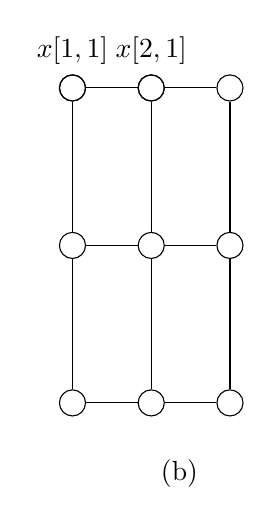
\begin{tikzpicture}
    \tikzset{x=1cm,y=2cm,every path/.style={>=latex},node style/.style={circle,draw}}
%    \node [minimum width=0.05cm]   (x1) at (-1,0)  {};     
%    \node [circle,minimum width=0.05cm,draw,label={$x[i]$}]   (x3) at (1,0)  {};  
%    \node [circle,minimum width=0.05cm,draw,label={$x[i\!+\!1]$}]   (x4) at (2,0)  {};         
%    \node [minimum width=0.05cm]   (x5) at (3,0)  {};          
%    \draw[line width=0.4,-,dashed] (x1) edge (x2);
%    \draw[line width=0.4,-] (x2) edge (x3);
%    \draw[line width=0.4,-] (x3) edge (x4);
%    \draw[line width=0.4,-,dashed] (x4) edge (x5);
      \foreach \x in {0,...,2}
       \foreach \y in {0,...,2} 
       { \node [circle,minimum width=0.05cm,draw]   (xy\x\y) at (\x,\y)  {}; 
       } 
  \foreach \x in {0,...,2}
   \foreach \y [count=\yi] in {0,...,1}  
      {\draw (xy\x\y)--(xy\x\yi) (xy\y\x)--(xy\yi\x) ;}
     
          \node [circle,minimum width=0.05cm,draw,label={$x[1,1]$}]   (x2) at (0,2)  {};
            \node [circle,minimum width=0.05cm,draw,label={$x[2,1]$}]   (x2) at (1,2)  {};
     \coordinate [label=45:(b)] (A) at (1,-0.6);\end{tikzpicture}
\end{minipage}

\vspace*{6mm}

\begin{minipage}[b]{.8\textwidth} 
\begin{center}
\begin{tikzpicture}
    \tikzset{x=0.5cm,y=3cm,every path/.style={>=latex},node style/.style={circle,draw}}
      \csvreader[ head to column names]%
                {NodesKarate.tex}{}{% 
     \coordinate[] (\nodeID) at (\a,\b);
     \draw [fill=white] (\nodeID) circle (2pt);
    }
     \draw [fill=white] (12) circle (2pt) node [above=2mm] {$x[i]$};
      \csvreader[ head to column names]%
                {EdgesKarate.tex}{}{%
    \draw[line width=0.3,-] (\a) edge (\b);
    } 
          \csvreader[ head to column names]%
                {NodesKarate.tex}{}{%
    \node [fill=white,circle,minimum width=0.05cm,draw]   (\nodeID) at (\a,\b)  {};     
    } 
       \coordinate [label=45:(c)] (A) at (3,1);
\end{tikzpicture}
\end{center}
\end{minipage}
\end{center}
\caption{\label{fig_graph_signals} Examples for the empirical graph of 
	networked data. (a) Chain graph representing signal amplitudes of 
	discrete time signals.  (b) Grid graph representing pixels of 2D-images. 
	(c) Empirical graph $\graph\!=\!(\nodes,\edges,\mW)$ for a dataset obtained 
from the social relations between members of a Karate club \cite{Zachary77}. 
The empirical graph with $\samplesize$ nodes $i \!\in\!\nodes\!=\!\{1,\ldots,\samplesize \}$ 
represents $\samplesize$ individual club members. Two nodes $i,j\!\in\!\nodes$ 
are connected by an edge $\{i,j\}\!\in\!\edges$ if the corresponding club members 
have interacted outside the club.}
\end{figure}



%Some important ML applications involve datasets which can be represented efficiently by an {\bf empirical graph} $\graph\!=\!(\nodes,\edges)$ 
%whose nodes $\nodes$ represent individual datapoints $\vx^{(\sampleidx)}$. For example, the node $i \!\in\! \nodes$ might represent a (super-)pixel in 
%image processing, a neuron of a neural network \cite{Goodfellow-et-al-2016} or a social network user profile \cite{BigDataNetworksBook}. 
%
%These applications naturally suggest a notion of similarity between individual datapoints, e.g., the profiles of 
%befriended social network users or greyscale values of neighbouring image pixels. These domain-specific 
%notions of similarity are represented by the edges of the empirical graph $\graph$, i.e., the nodes $i,j\!\in\!\nodes$ 
%representing similar datapoints $\vx^{(i)}$ and $\vx^{(j)}$ are connected by an undirected edge $\{i,j\}\!\in\!\edges$. We denote 
%the neighbourhood of the node $i\in \nodes$ by $\mathcal{N}(i) \defeq \{ j \in \nodes: \{i,j\} \in \edges \}$. 
%
%In some applications it is possible to quantify the extent to which datapoints $\vx^{(i)}$ and $\vx^{(j)}$ are similar, e.g., via the Euclidean distance 
%$\| \vx^{(i)} -  \vx^{(j)} \|$. Given two similar datapoints $i,j\!\in\!\nodes$, which are connected by an edge $\{i,j\} \in \edges$, 
%we will quantify the strength of their connection by the edge weight $W_{i,j}\!>\!0$ which we collect 
%in the symmetric weight matrix $\mathbf{W} \in \mathbb{R}_{+}^{\samplesize \times \samplesize}$. The 
%absence of an edge between nodes $i,j \in \nodes$ is encoded by a zero weight $W_{i,j}\!=\!0$. 
%Thus the edge structure of the empirical graph $\graph$ is fully specified by the support (locations of 
%the non-zero entries) of the weight matrix $\mathbf{W}$. 

Besides the empirical graph structure $\graph$, a dataset 
typically conveys additional information, e.g., features, labels 
or model parameters. We can represent this additional 
information by a graph signal defined over $\graph$. 
A graph signal $h[\cdot]$ is a map $\nodes \rightarrow \mathbb{R}$, 
which associates every node $i\!\in\!\nodes$ with the signal 
value $h[i] \!\in\! \mathbb{R}$. 

The graph signals arising in several important application domains can 
be well modelled using a cluster assumption \cite{SemiSupervisedBook}. 
The cluster assumption requires similar signal values $h[i] \approx h[j]$ 
at nodes $i,j \in \nodes$, which belong to the same well-connected 
subset of nodes (``cluster'') of the empirical graph. The clusteredness 
of a graph signal $h[\cdot]$ can be measured by the total variation (TV): 
\begin{equation}
\label{equ_def_TV}
 \| h \|_{\rm TV} = \sum_{\{i,j\} \in \edges} W_{i,j} |h(i) - h(j)|. 
\end{equation} 
 
Clustered graph signals arise in digital signal processing which 
studies graph signals defined over the chain graph representing 
discrete time instants. 

The signal values at adjacent time instants are correlated 
for sufficiently high sampling rate. Image processing methods 
use the tendency of close-by pixels to be coloured likely 
which amounts to a clustered graph signal over a grid 
graph representing pixels of a 2D image.  

The recently introduced network Lasso (nLasso) amounts to a formal ML problem involving 
network-structured data which can be represented by an empirical graph $\graph$. In particular, 
the hypothesis space of nLasso is constituted by graph signals on $\graph$: 
\begin{equation}
\hypospace  = \{ h: \nodes \rightarrow \labelspace \}.
\end{equation} 
The loss function of nLasso is a combination of squared error and TV (see \eqref{equ_def_TV}) 
\begin{equation}
\loss{(\vx,y)}{h} = (y - h(\vx))^{2} + \lambda \| h  \|_{\rm TV}. 
\end{equation} 
Choosing a small value for the regularization parameter $\lambda$ put more emphasis 
on a small prediction error $y-h(\vx)$. Using a large value for $\lambda$ favours clustered 
hypothesis $h$, which is constant over well-connected subsets of nodes. 


{\bf Logistic Network Lasso.} The logistic network Lasso \cite{LogisticNLassoAsilomar2018,LogisticNLasso} 
is a modification of the network Lasso (see Section \ref{sec_network_lasso}) for classification problems 
involving partially labeled networked data represented by an empirical graph $\graph=(\nodes,\edges,\mathbf{W})$. 

Each datapoint $\vz$ is characterized by the features $\vx$ and is associated with a label $y \in \labelspace$, 
taking on values from a discrete label space $\labelspace$. The simplest setting is binary classification where 
each datapoint has a binary label $y \in \{-1,1\}$. The hypothesis space underlying logistic network Lasso 
is given by the graph signals on the empirical graph: 
\begin{equation}
\hypospace  = \{ h: \nodes \rightarrow \labelspace \}
\end{equation} 
and the loss function is a combination of logistic loss and TV (see \eqref{equ_def_TV})
\begin{equation}
\loss{(\vx,y)}{h} = -\log(1+ \exp(-yh(\vx))) + \lambda \| h  \|_{\rm TV}. 
\end{equation} 

\section{Exercises}

\subsection{How Many Neurons?} 
\label{exercise_how_many_neurons} 
Consider a predictor map $h(x)$ which is piece-wise linear and consisting 
of $1000$ pieces. Assume we want to represent this map by an ANN using 
neurons with ReLU activation functions. How many neurons must the ANN 
at least contain?

\subsection{Linear Classifiers} 
\label{exercise_linear_classifier} 
Consider datapoints characterized by feature vectors $\vx \in \mathbb{R}^{n}$ and 
binary labels $y \in\{-1,1\}$. We are interested in finding a good linear classifier which is such that 
the feature vectors resulting in $h(\vx) = 1$ is a half-space. Which of the methods 
discussed in this chapter aim at learning a linear classifier?


\subsection{Data Dependent Hypothesis Space} 
\label{exercise_data_dep_hypospace} 
Which of the following ML methods uses a hypothesis space that 
depends on the training data. 
\begin{itemize} 
	\item logistic regression 
	\item linear regression 
	\item k-NN 
\end{itemize}


\newpage
\chapter{Empirical Risk Minimization}
\label{ch_Optimization}

\begin{figure}[htbp]
\begin{center}
    \begin{tikzpicture}
          \begin{axis}
          [ylabel= {},
              xlabel={predictor $h\in \hypospace$},%grid, 
              axis x line=center,
  axis y line=center,
  yscale=1.2,
  xscale=1.2,  
  xtick=\empty,
  ytick=\empty,
 % ytick={0,1,...,2},
 % xlabel={prediction error $y-h(x)$},
  %ylabel={squared error loss $\mathcal{L}$},
  xlabel style={below right},
  ylabel style={above},
  xmin=-2.5,
  xmax=2.5,
  ymin=-0.1,
  ymax=1.2
  ]
              % \addplot [smooth, color=red, ultra thick] table [x=a, y=b, col sep=comma] {logloss.csv};    
            %       \addplot [color=blue, ultra thick] table [x=a, y=b, col sep=comma] {hingeloss.csv};     
\addplot [color=black, ultra thick,dashed] table [x=a, y=b, col sep=comma] {averagepredloss.csv};      
\addplot [color=black, ultra thick] table [x=a, y=b, col sep=comma] {emprisk.csv};      
\end{axis}
  \node [right] at (6.5,3.7) {average prediction error};
  \node [above] at (0,5.8) {empirical risk};
           %\node [left,color=blue] at (3.1,1.5) {hinge loss (for $y\!=\!1)$};
          % \node [left] at (1.5,3) {$0/1$ loss (for $y\!=\!1)$};
     \end{tikzpicture}
     \vspace*{-4mm}
\end{center}
\caption{ML methods aim at learning a predictor $h \in \hypospace$ that incurs 
	small loss on any datapoint. Empirical risk minimization approximates the
    expected loss or risk with the empirical risk (solid curve) incurred on a 
    finite set of labeled datapoints (the training set).}
\label{fig_ERM_idea}
\end{figure}


Chapter \ref{ch_Elements_ML} explained three components of ML (see Figure \ref{fig_ml_problem}): 
\begin{itemize} 
\item the feature space $\featurespace$ and label space $\labelspace$, 
\item a hypothesis space $\hypospace$ of computationally feasible predictor maps $\featurespace \rightarrow \labelspace$, 
\item and a loss function $\loss{(\vx,y)}{h}$ which measures the discrepancy between the predicted label $h(\vx)$ and 
the true label $y$ of a datapoint. $ error $ incurred by predictor $h \in \hypospace$. 
\end{itemize} 
Ideally we would like to learn a hypothesis $h$ out of the model $\hypospace$ 
such that $h(\vx) \approx y$ or, in turn,  $\loss{(\vx,y)}{h}$ is very small, 
for any datapoint $(\vx,y)$. However, in practice we can only use a given 
set of labeled datapoints (the training set) to measure the average loss 
of a hypothesis $h$. 

How can we know the loss of a hypothesis $h$ when predicting the label 
of datapoints outside the training set? One possible approach is to use 
a {\bf probabilistic model} for the data. In this model, we interpret datapoints 
as realizations of i.i.d. random variables with the (same) probability distribution 
$p(\vx,y)$. The training set is one particular set of such realizations drawn 
from $p(\vx,y)$. Moreover, we can generate datapoints outside the training 
set by drawing realizations from the distribution $p(\vx,y)$. Given this probability 
distribution over different realizations of datapoints allows to define the risk 
of a hypothesis $h$ as the expectation of the loss incurred by $h$ on a 
random datapoint. 

If we would know the probability distribution $p(\vx,y)$, from which the datapoints 
are drawn, we could minimize the risk using probability theory. 
Roughly speaking, the optimal hypothesis $h$ can be read directly from the 
posterior probability distribution $p(y|\vx)$ of the label $y$ 
given the features $\vx$ of a datapoint. When using the squared error loss, 
the risk is minimized by the hypothesis $h(\vx) = \expect \big\{ y | \vx \}$. 

In practice we do not know the true underlying probability 
distribution and have to estimate it from data. Therefore, 
we cannot compute the Bayes' optimal estimator exactly. 
However, we can approximately compute this estimator 
by replacing the exact probability distribution with an 
estimate. Moreover, the risk of the Bayes' optimal estimator 
provides a useful benchmark against which we can compare 
the average loss of practical ML methods. 

Section \eqref{equ_sec_emp_risk_approximates_expected_loss} formally 
defines the risk of a hypothesis and motivates empirical risk minimization (ERM) 
as a natural approximation of the risk using labeled (training) datapoints. 
We then specialize the ERM for three particular ML problems. These three 
ML problems use different combinations of model (hypothesis space) and 
loss functions which result in ERM with different computational complexities. 

In Section \ref{sec_ERM_lin_reg}, we discuss the ERM obtained for linear 
regression (see Section \ref{sec_lin_regression}). The resulting ERM amounts 
to minimizing a differentiable convex function, which can be done efficiently 
using gradient-based methods (see Chapter \ref{ch_GD}). 

We then discuss in Section \ref{sec_ERM_decision_tree} the ERM 
obtained for decision tree models. The resulting ERM becomes a 
discrete optimization problem which are typically much harder than 
convex optimization problems. We cannot apply gradient-based methods 
to solve the ERM for decision trees. To solve the decision tree ERM we 
essentially must try out all possible choices for the tree structure \cite{}. 

Section \ref{sec_ERM_Bayes} considers the ERM obtained when learning a linear hypothesis 
using the $0/1$ loss for classification problems. The resulting ERM 
amounts to minimizing a non-differentiable and non-convex function. 
Instead of using computationally expensive methods for minimizing 
this function, we will use a different rout via probability theory to 
construct approximate solutions to this ERM instance. 

As explained in Section \ref{sec_training_inference}, many ML methods 
use the ERM during a training period to learn a hypothesis which is 
then applied to new datapoints during the inference period. 
Section \ref{sec_online_learning} demonstrates how an online 
learning method can be obtained by solving the ERM sequentially 
as new datapoints come in. Online learning methods continuously 
alternate between training and inference periods. 


%Let us now see how the construction of Bayes' 
%optimal predictors can 
%be adapted to obtain practical ML methods. 

\section{Why Empirical Risk Minimization?} 
\label{equ_sec_emp_risk_approximates_expected_loss}

We assume that datapoints are i.i.d.\ realizations drawn from some fixed 
probability distribution $p(\vx,y)$. The probability distribution $p(\vx,y)$ 
allows us to define the {\bf expected loss} or {\bf risk} 
\begin{equation}
\label{equ_def_risk} 
\expect \big \{ \loss{(\vx,y)}{h} \}.
\end{equation}
Many ML methods learn a predictor out of $\hypospace$ such 
that \eqref{equ_def_risk} is minimal. 

If we would know the probability distribution of the data, we could 
in principle readily determine the best predictor map by solving an 
optimization problem. This optimal predictor is known as the Bayes' 
predictor and depends on the probability distribution $p(\vx,y)$ 
and the loss function. For the squared error loss, the Bayes' 
predictor is the posterior mean of $y$ given the features $\vx$. 

We often do not know the probability distribution and therefore 
cannot evaluate the expectation in \eqref{equ_def_risk}. 
%However, we can 
%estimate the expectation using an empirical average over a set of 
%datapoints (``training data''). 
%Many ML methods are optimization methods that use the empirical 
%risk on the training data as an estimate for the average (expected) 
%error. Thus, in contrast to standard optimization methods, these 
%ML methods optimize an estimate - or approximation - of the actual 
%objective function \eqref{equ_def_risk}. 
%A key idea underlying many ML methods is to find (learn) a predictor map with small empirical risk, 
%which serves as a proxy for the average prediction error. The resulting ML methods are optimization 
 {\bf ERM} replaces the expectation in  \eqref{equ_def_risk} with an average 
 over a given set of labeled datapoints,  
\begin{align}
\label{equ_def_ERM_funs}
   \hat{h} & = \argmin_{h \in \hypospace} \emperror(h|\dataset) \nonumber \\ 
   & \stackrel{\eqref{eq_def_emp_error_101}}{=}  \argmin_{h \in \hypospace} (1/\samplesize) \sum_{\sampleidx=1}^{\samplesize} \loss{(\vx^{(\sampleidx)},y^{(\sampleidx)})}{h}.
\end{align}
The ERM \eqref{equ_def_ERM_funs} amounts to learning (finding) a 
good predictor $\hat{h} \in \hypospace$ by ``training'' it on the 
dataset $\dataset = \{ (\vx^{(\sampleidx)},y^{(\sampleidx)}) \}_{\sampleidx=1}^{\samplesize}$, 
which is therefore referred to as the {\bf training set}. 

\section{Computational and Statistical Aspects of ERM}
\label{sec_comp_stat_ERM}

\emph{Statistical Aspects: Objective in ERM is Noisy version of Actual Objective; sometimes we do 
not know most parts of objective function (reinforcement learning); even if we know 
the objective function (expected risk) perfectly, optimization might be hard for non-smooth, 
non-convex objective functions}

Solving the optimization problem \eqref{equ_def_ERM_funs} provides 
two things. First, the minimizer $\hat{h}$ is a predictor which performs 
optimal on the training set $\dataset$. Second, the corresponding 
objective value $\emperror(\hat{h}|\dataset)$ (the ``training error'') 
indicates how accurate the predictions of $\hat{h}$ will be. 

As we will discuss in Chapter \ref{ch_overfitting_regularization}, for some 
datasets $\dataset$, the training error $\emperror(\hat{h}|\dataset)$ obtained 
for $\dataset$ can be very different from the average prediction error of $\hat{h}$ 
when applied to new datapoints which are not contained in $\dataset$. 

%????I would like that the "equivalent to find optimum weight vertoc w0" from slide Optimal Linear Regression would be explained again. The mathematical notation used there isn't that familiar for me.?????
%Consider, e.g., the hypothesis space $\hypospace$ of linear predictors is based on a parametrization of the hypothesis $h(\vx^{(\timeidx)})$. 
Many important ML methods use hypotheses that are parametrized by 
weight vector $\vw$. For each possible weight vector, we obtain a 
hypothesis $h^{(\vw)}(\vx)$. Such a parametrization is used in linear 
regression which learns a linear hypotheses $h(\vx) = \vw^{T} \vx$ with 
some weight vector $\vw$. Another example for such a parametrization 
are ANNs with the weights assigned to inputs of individual neurons (see Figure \ref{fig_ANN}). 

For ML methods that use a parameterized hypothesis $h^{(\vw)}(\vx)$, 
we can reformulate the optimization problem \eqref{equ_def_ERM_funs} 
as an optimization of the weight vector, 
\begin{equation}
\label{eq_def_ERM_weight}
    \vw_{\rm opt} = \argmin_{\vw \in \mathbb{R}^{\featuredim}} f(\vw) \mbox{ with } f(\vw) \defeq(1/\samplesize) \sum_{\sampleidx=1}^{\samplesize} \loss{(\vx^{(\sampleidx)},y^{(\sampleidx)})}{h^{(\vw)}}. 
\end{equation}
The objective function $f(\vw)$ in \eqref{eq_def_ERM_weight} is 
the empirical risk $\emperror\big(h^{(\vw)} |\dataset\big)$ incurred  
by the hypothesis $h^{(\vw)}$ when applied to the datapoints in the dataset $\dataset$. 

The optimization problems \eqref{eq_def_ERM_weight} and \eqref{equ_def_ERM_funs} 
are fully equivalent. Given the optimal weight vector $\vw_{\rm opt}$ solving 
\eqref{eq_def_ERM_weight}, the predictor $h^{(\vw_{\rm opt})}$ is 
an optimal predictor solving \eqref{equ_def_ERM_funs}. 

Learning a hypothesis via ERM \eqref{equ_def_ERM_funs} is a form of 
learning by ``trial and error''. An instructor (or supervisor) provides some 
snapshots $\vz^{(\sampleidx)}$ which are characterized by features 
$\vx^{(\sampleidx)}$ and associated with known labels $y^{(\sampleidx)}$. 

The learner then uses a hypothesis $h$ to guess the labels $y^{(\sampleidx)}$ 
only from the features $\vx^{(\sampleidx)}$ of all training data points. We then 
determine average loss or training error $\emperror(h|\dataset)$ that is incurred 
by the predictions $\hat{y}^{(\sampleidx)} = h\big( \vx^{(\sampleidx)} \big)$. 
If the error $\emperror(h|\dataset)$ is too large, we should try out another  
hypothesis map $h'$ different from $h$ with the hope of achieving a smaller 
training error $\emperror(h'|\dataset)$. 

%This principle of learning by supervision, using labeled datapoints (``training examples''), 
%could also be used to model the development of language in human brains (``concept learning''). Consider a 
%child, who should learn the concept ``tractor'' (see Figure \ref{fig_tractors}). We could try to show 
%many different pictures to the child and for each picture say ``tractor'' or ``no tractor''. Based on this 
%``labeled data'', the child tries to learn the relation between features of an image and the presence 
%(or absence) of a tractor in the image. 
%
%\begin{figure}[htbp]
%    \centering
%    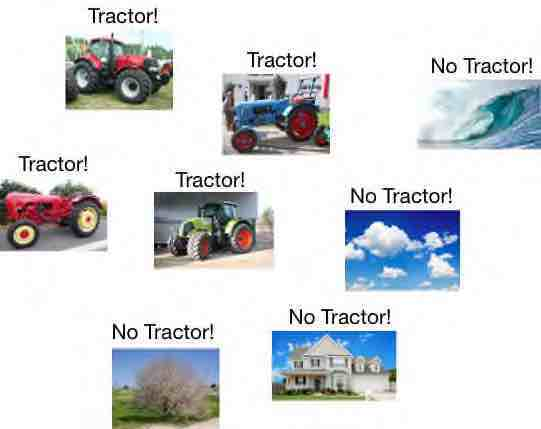
\includegraphics[width=0.7\textwidth]{LabeledDataTractor1.jpg}  
%    \label{fig_tractors}
%        \caption{A bunch of labeled images. The label $y$ of an image indicates if a tractor is shown ($y=1$) or not ($y=-1$).}
%\end{figure}

We highlight that the precise shape of the objective function 
$f(\vw)$ in \eqref{eq_def_ERM_weight} depends heavily on the 
parametrization of the predictor functions, i.e., how does the 
predictor $h^{(\vw)}$ vary with the weight vector $\vw$. 

The shape of $f(\vw)$ depends also on the choice for the loss 
function $\loss{(\vx^{(\sampleidx)},y^{(\sampleidx)})}{h}$. As 
depicted in Figure \ref{fig_diff_types_bojec}, the different combinations 
of predictor parametrisation and loss functions can result in objective 
functions with fundamentally different properties such that their 
optimization is more or less difficult. 

The objective function $f(\vw)$ for the ERM obtained for linear 
regression (see Section \ref{sec_lin_regression}) is differentiable 
and convex and can therefore be minimized using simple 
gradient based  methods (see Chapter \ref{ch_GD}). In contrast, 
the objective function $f(\vw)$ of ERM obtained for the SVM (see 
Section \ref{sec_SVM}) is non-differentiable but still convex. The 
minimization of such functions is more challenging but still tractable 
as there exist efficient convex optimization methods which do not 
require differentiability of the objective function \cite{ProximalMethods}. 

The objective function $f(\vw)$ obtained for ANN are typically 
{\bf highly non-convex} having many local minima. The optimization 
of non-convex objective function is in general more difficult than 
optimizing convex objective functions. However, it turns out that 
despite the non-convexity, iterative gradient-based methods can 
still be successfully applied to solve the ERM \cite{Goodfellow-et-al-2016}. 
Even more challenging is the ERM obtained for decision trees or 
Bayes' classifiers. These ML problems involve non-differentiable 
and non-convex objective functions. 


	
\begin{figure}[htbp]
\begin{center}
\scalebox{0.8}{
    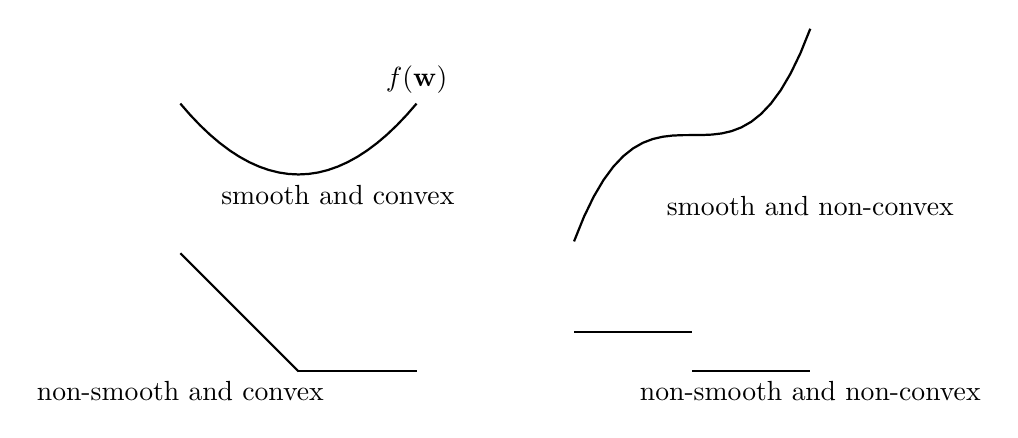
\begin{tikzpicture}[scale=0.5]
       %   \begin{axis}
       %   [ylabel=$h(x)$,
         %     xlabel=$x$,grid]
             %  \addplot table [x=a, y=b, col sep=comma] {data.csv};      
                 \draw[thick, domain=-3:3]  node[left=2cm,below] {smooth and convex} plot ({\x-5},  {0.2*\x*\x}) node [above] {$f(\vw)$} ;
                         \draw[thick, domain=-3:3] plot ({\x+5},  {0.1*\x*\x*\x +1}) node[below=2cm] {smooth and non-convex} ;                   
                   \draw[thick, domain=-3:0] plot ({\x-5},  {-\x-5}) ;
                     \draw[thick, domain=0:3] plot ({\x-5},  {-5}) node[left=3cm,below] {non-smooth and convex};
                          \draw[thick, domain=-3:0] plot ({\x+5},  { -4})  ;         
                               \draw[thick, domain=0:3] plot ({\x+5},  { -5}) node[below] {non-smooth and non-convex} ;         
%                 \draw[blue,  thick, domain=-1:0] plot (\x,  {1+\x}); 
%                 \draw[blue,  thick, domain=0:1] plot (\x,  {1-\x});    
%                   \draw[blue,  thick, domain=1:3] plot (\x,  {0});           
%          \draw[->] (-3.5,0) -- (3.5,0) node[right] {$x$};
%   \draw[->] (0,-0.25) -- (0,1.5) node[above] {$h^{(\vw)}(x)$};
%           %      \draw[dashed, thick, domain=1:3.6] plot (\x,  {\x - 1}) node[right] {$ f(\vw_{0})\!+\!(\vw\!-\!\vw_{0})^{T} \nabla f(\vw_{0})$};
%                    \foreach \y/\ytext in {0/0, 1/1}
%    \draw[shift={(0,\y)}] (2pt,0pt) -- (-2pt,0pt) node[left] {$\ytext$};  
%                        \foreach \x/\xtext in {-3/-3,-2/-2,-1/-1,0/0,1/1, 2/2,3/3}
%    \draw[shift={(\x,0)}] (0pt,2pt) -- (0pt,-2pt) node[below] {$\xtext$};  
%       %   \end{axis}
     \end{tikzpicture}}
\end{center}
\caption{Different types of objective functions obtained for ERM in different settings.}
\label{fig_diff_types_bojec}
\end{figure}

\section{ERM for Linear Regression}
\label{sec_ERM_lin_reg}

As discussed in Section \ref{sec_lin_regression}, linear regression methods 
learn a linear hypothesis $h^{(\vw)}(\vx) = \vw^{T} \vx$ with minimum squared 
error loss \eqref{equ_squared_loss}. For this choices, the ERM problem \eqref{eq_def_ERM_weight} 
specializes to  
\begin{align}
\label{equ_def_cost_MSE}
\vw_{\rm opt} & = \argmin_{\vw \in \mathbb{R}^{\featuredim}} f(\vw) \nonumber \\ 
& \mbox{ with } f(\vw)\!\defeq\!(1/\samplesize) \sum_{(\vx,y)\!\in\!\dataset} (y \!-\! \vx^{T} \vw )^2.
\end{align} 
Here, $\samplesize=|\dataset|$ denotes the (sample) size of the training set $\dataset$. 
The objective function $f(\vw)$ in \eqref{equ_def_cost_MSE} is computationally 
appealing since it is a convex and smooth function. Such a function can be minimized 
efficiently using the gradient-based methods discussed in Chapter \ref{ch_GD}. 

The ERM problem \eqref{equ_def_cost_MSE} can rewritten in a more compact form 
by stacking the labels $y^{(\sampleidx)}$ and feature vectors $\vx^{(\sampleidx)}$, for 
$\sampleidx=1,\ldots,\samplesize$, into a ``label vector'' $\vy$ and ``feature matrix'' $\mX$, 
\begin{align}
\label{equ_def_vec_matrix}
\mathbf{y} & = ( y^{(1)},\ldots, y^{(\samplesize)})^{T} \in \mathbb{R}^{\samplesize} \mbox{, and } \nonumber \\ 
\mathbf{X} & = \begin{pmatrix} \vx^{(1)},\ldots,\vx^{(\samplesize)} \end{pmatrix}^{T}\in \mathbb{R}^{\samplesize \times \featuredim}.
\end{align}
This allows to rewrite the objective function in \eqref{equ_def_cost_MSE} as 
\begin{equation}
\label{equ_min_lin_pred_vec_mat}
f(\vw) = (1/\samplesize) \| \vy - \mX\vw \|^{2}_{2}.
\end{equation} 

Inserting \eqref{equ_min_lin_pred_vec_mat} into \eqref{equ_def_cost_MSE}, 
we obtain the quadratic problem 
\begin{align}
\label{equ_quadr_form_linreg}
& \min_{\vw \in \mathbb{R}^{\featuredim}} \underbrace{(1/2) \vw^{T} \mathbf{Q} \vw - \vq^{T}  \vw}_{= f(\vw)} \nonumber \\
& \mbox{ with } \mathbf{Q}= (1/\samplesize) \mathbf{X}^{T} \mathbf{X}, \mathbf{q} =(1/\samplesize) \mathbf{X}^{T} \mathbf{y}. 
\end{align} 
Since $f(\vw)$ is a differentiable and convex function, a necessary and sufficient condition for 
$\vw_{\rm opt}$ to be a minimizer $f(\vw_{\rm opt})\!=\!\min_{\vw \in \mathbb{R}^{\featuredim}} f(\vw)$ is the 
{\bf zero-gradient condition} \cite[Sec. 4.2.3]{BoydConvexBook}
\begin{equation}
\label{equ_zero_gradient}
 \nabla f(\vw_{\rm opt}) = \mathbf{0}.
\end{equation} 

Combining \eqref{equ_quadr_form_linreg} with \eqref{equ_zero_gradient}, 
yields the following sufficient and necessary condition for a weight vector 
$\vw_{\rm opt}$ to solve the ERM \eqref{equ_def_cost_MSE},
\begin{equation}
\label{equ_zero_gradient_lin_reg}
(1/\samplesize) \mX^{T} \mX \vw_{\rm opt} = (1/\samplesize) \mX^{T} \vy.  
\end{equation} 
This condition can be rewritten as 
\begin{equation}
\label{equ_zero_gradient_lin_reg_normal_condition}
(1/\samplesize) \mX^{T} \big( \vy - \mX \vw_{\rm opt} \big) = \mathbf{0}.  
\end{equation} 
We might refer to this condition as ``normal equations'' as they 
require the vector $$\big( \vy - \mX \vw_{\rm opt} \big) = \big(\big(y^{(1)}-\hat{y}^{(1)}\big),\ldots,\big(y^{(\samplesize)}-\hat{y}^{(\samplesize)}\big)  \big)^{T},$$
whose entries are the prediction errors for the training datapoints, to 
be orthogonal (or normal) to the subspace spanned by the columns 
of the feature matrix $\mathbf{X}$. 


It can be shown that, for any given feature matrix $\mX$ and label vector $\vy$, there always 
exists at least one optimal weight vector $\vw_{\rm opt}$ which solves \eqref{equ_zero_gradient_lin_reg}. 
The optimal weight vector might not be unique, such that there are several different vectors 
which achieve the minimum in \eqref{equ_def_cost_MSE}. However, 
every vector $\vw_{\rm opt}$ which solves \eqref{equ_zero_gradient_lin_reg} 
achieves the same minimum empirical risk 
\begin{equation}
\label{equ_emp_risk_lin_proje}
\emperror(h^{(\vw_{\rm opt})} \mid \dataset) = \min_{\vw \in \mathbb{R}^{\featuredim}} \emperror(h^{(\vw)} \mid \dataset) = \|  (\mathbf{I}- \mathbf{P}) \vy \|^{2}.
\end{equation} 
Here, we used the orthogonal projection matrix $\mathbf{P} \in \mathbb{R}^{\samplesize \times \samplesize}$ 
on the linear span of the feature matrix $\mX = (\vx^{(1)},\ldots,\vx^{(\samplesize)})^{T} \in \mathbb{R}^{\samplesize \times \featuredim}$ (see \eqref{equ_def_vec_matrix}).\footnote{The linear span of a matrix $\mA=(\va^{(1)},\ldots,\va^{(\samplesize)}) \in \mathbb{R}^{\featuredim \times \samplesize}$, denoted as ${\rm span } \big\{\mA\}$, is the subspace 
	of $\mathbb{R}^{\featuredim}$ consisting of all linear combinations 
of the columns $\va^{(r)} \in \mathbb{R}^{\featuredim}$ of $\mA$.} 

If the feature matrix $\mX$ (see \eqref{equ_def_vec_matrix}) has full column rank, 
which implies that the matrix $\mX^{T} \mX$ is invertible, the projection matrix $\mathbf{P}$ 
is given explicitly as 
\begin{equation} 
\nonumber
\mathbf{P} = \mX \big( \mX^{T} \mX \big)^{-1} \mX^{T}. 
\end{equation} 
Moreover, the solution of \eqref{equ_zero_gradient_lin_reg} is then unique and given by 
\begin{equation}
\label{equ_close_form_lin_reg}
\vw_{\rm opt} = \big(  \mX^{T} \mX \big)^{-1} \mX^{T} \vy. 
\end{equation}
The closed-form solution \eqref{equ_close_form_lin_reg} requires 
the inversion of the $\featuredim \times \featuredim$ matrix $\mX^{T} \mX$. 

Computing the inverse of $\mX^{T} \mX$ can be computationally challenging 
for large number $\featuredim$ of features. Figure \ref{fig_snapshot_pixels} 
depicts a simple ML problem where the number of features is already 
in the millions. The inversion of the matrix $\mX^{T} \mX$ is particularly 
challenging if this matrix is ill-conditioned. In general, we do not have 
any control on this condition number as we face datapoints with arbitrary 
feature vectors. 

Section \ref{sec_lin_reg} discusses a method for computing the optimal weight vector 
$\vw_{\rm opt}$ which does not require any matrix inversion. This method, 
referred to as {\bf gradient descent}, constructs a sequence 
$\vw^{(0)}, \vw^{(1)},\ldots$ of increasingly accurate approximations 
of $\vw_{\rm opt}$. This iterative method has two major benefits 
compared to evaluating the formula \eqref{equ_close_form_lin_reg} using 
direct matrix inversion, such as Gauss-Jordan elimination \cite{golub96}. 
First, gradient descent requires much fewer arithmetic operations compared 
to direct matrix inversion. This is crucial in modern ML applications involving 
large feature matrices. Second, gradient descent does not break when the 
matrix $\mX$ is not full rank and the formula \eqref{equ_close_form_lin_reg} 
cannot be used any more. 

\section{ERM for Decision Trees}
\label{sec_ERM_decision_tree}

Consider the ERM problem \eqref{equ_def_ERM_funs} for a regression 
problem with label space $\labelspace=\mathbb{R}$, feature space 
$\featurespace= \mathbb{R}^{\featuredim}$ and using a hypothesis 
space defined by decision trees (see Section \ref{sec_decision_trees}). 

In stark contrast to the ERM problem obtained for linear or logistic 
regression, the ERM problem obtained for decision trees amounts 
to a {\bf discrete optimization problem}. Consider the particular 
hypothesis space $\hypospace$ depicted in Figure \ref{fig_hypospace_DT_depth_2}. 
This hypothesis space contains a finite number of predictor maps, 
each map corresponding to a particular decision tree. 

For the small hypothesis space $\hypospace$ in Figure \ref{fig_hypospace_DT_depth_2}, 
ERM is easy. Indeed, we just have to evaluate the empirical risk 
for each of the elements in $\hypospace$ and pick the one yielding 
the smallest empirical risk. However, for increasing size of decision 
trees the computational complexity of exactly solving the ERM becomes 
intractable. 

A popular approach to ERM for decision trees is to use greedy algorithms which try to expand (grow) 
a given decision tree by adding new branches to leaf nodes in order to reduce the empirical risk 
(see \cite[Chapter 8]{IntroSLR} for more details). 

\begin{center}
\framebox[0.96\textwidth]{
 \parbox{0.9\textwidth}{
The idea behind many decision tree learning methods is quite simple: try out expanding a decision tree by 
replacing a leaf node with a decision node (implementing another ``test'' on the feature vector) in order to 
reduce the overall empirical risk as much as possible. 
}}
\end{center}

Consider the labeled dataset $\dataset$ depicted in Figure \ref{fig_growingatree} and a given decision tree for 
predicting the label $y$ based on the features $\vx$. We start with a very simple tree shown in the top of 
Figure \ref{fig_growingatree}. Then we try out growing the tree by replacing a leaf node with a decision node. 
According to Figure \ref{fig_growingatree}, replacing the right leaf node results in a decision tree which is 
able to perfectly represent the training dataset (it achieves zero empirical risk). 
 
 

\begin{figure}[htbp]
\begin{center}
\begin{minipage}{0.4\textwidth}
\scalebox{0.8}{
\begin{tikzpicture}[auto,scale=0.8]
%\draw [thick] (-3,-3) rectangle (1,4) node [anchor=east,above] {$\featurespace$} ;
\draw [thick] (5,5) circle (0.1cm)node[anchor=west] {\hspace*{0mm}$\vx^{(3)}$};
%\draw [dashed] (3,3) rectangle (6,6) ;
%\draw [dashed] (3,0) rectangle (6,3) ;
%\draw [dashed] (0,3) rectangle (3,6) ;
\draw [dashed] (0,0) rectangle (3,6) ;
\draw [dashed] (3,0) rectangle (6,6) ;
\draw [thick] (1,1) circle (0.1cm)node[anchor=west] {\hspace*{0mm}$\vx^{(4)}$};
%\draw [thick] (-2,-1.7) circle (0.1cm)node[anchor=west] {\hspace*{0mm}$\vx^{(3)}$};
%\draw [thick] (2,-1.9) circle (0.1cm) node[anchor=west] {\hspace*{0mm}$\vx^{(2)}$};
\draw [thick] (5,1) circle (0.1cm)node[anchor=west,above] {\hspace*{0mm}$\vx^{(2)}$};
\draw [thick] (1,5) rectangle ++(0.1cm,0.1cm) node[anchor=west,above] {\hspace*{0mm}$\vx^{(1)}$};
\draw[->] (-0.5,0) -- (6.5,0) node[right] {$x_{1}$};
\draw[->] (0,-0.5) -- (0,6.5) node[above] {$x_{2}$};
\foreach \y/\ytext in {0/0, 1/1,2/2,3/3,4/4,5/5,6/6} \draw[shift={(0,\y)}] (2pt,0pt) -- (-2pt,0pt) node[left] {$\ytext$};  
\foreach \x/\xtext in{0/0, 1/1,2/2,3/3,4/4,5/5,6/6}\draw[shift={(\x,0)}] (0pt,2pt) -- (0pt,-2pt) node[below] {$\xtext$};  
\end{tikzpicture}}
\end{minipage}
\begin{minipage}{0.5\textwidth}
\scalebox{0.9}{
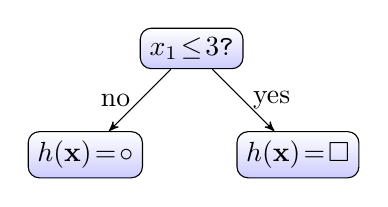
\begin{tikzpicture} [->,>=stealth',level/.style={sibling distance = 2cm/#1,
   level distance = 1.5cm},scale=0.9]
   \vspace*{-30mm} 
\tikzstyle{level 1}=[sibling distance=30mm]
  \tikzstyle{level 2}=[sibling distance=30mm]
\node [env] {$x_{1}\!\leq\!3$?}
child  {node [env] {$h(\vx)\!=\!\circ$} 
   % child {node [env] {$h(\vx)\!=\!y^{(3)}$}  edge from parent node [left,align=center] {no}}
   % child {node [env] {$h(\vx)\!=\!y^{(2)}$}   edge from parent node [left,align=center] {yes}}
  edge from parent node [left,align=center] {no} }
child { node [env]  {$h(\vx)\!=\!\Box$}
%   child {node [env] {$h(\vx)\!=\!y^{(1)}$}   edge from parent node [left,align=center] {no} }
  %  child {node [env] {$h(\vx)\!=\!y^{(4)}$}   edge from parent node [left,align=center] {yes} }
  edge from parent node [right,align=center] {yes}};
\end{tikzpicture}}
\end{minipage}
\end{center}
\vspace*{5mm}
\begin{minipage}{0.2\textwidth}
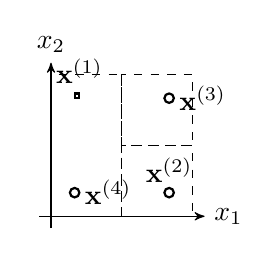
\begin{tikzpicture}[auto,scale=0.3]
%\draw [thick] (-3,-3) rectangle (1,4) node [anchor=east,above] {$\featurespace$} ;
\draw [thick] (5,5) circle (0.2cm)node[anchor=west] {\hspace*{0mm}$\vx^{(3)}$};
%\draw [dashed] (3,3) rectangle (6,6) ;
%\draw [dashed] (3,0) rectangle (6,3) ;
\draw [dashed] (3,0) rectangle (3,3) ;
\draw [dashed] (0,0) rectangle (3,6) ;
\draw [dashed] (3,0) rectangle (6,3) ;
\draw [dashed] (3,3) rectangle (6,6) ;
\draw [thick] (1,1) circle (0.2cm)node[anchor=west] {\hspace*{0mm}$\vx^{(4)}$};
%\draw [thick] (-2,-1.7) circle (0.1cm)node[anchor=west] {\hspace*{0mm}$\vx^{(3)}$};
%\draw [thick] (2,-1.9) circle (0.1cm) node[anchor=west] {\hspace*{0mm}$\vx^{(2)}$};
\draw [thick] (5,1) circle (0.2cm)node[anchor=west,above] {\hspace*{0mm}$\vx^{(2)}$};
\draw [thick] (1,5) rectangle ++(0.2cm,0.2cm) node[anchor=west,above] {\hspace*{0mm}$\vx^{(1)}$};
\draw[->] (-0.5,0) -- (6.5,0) node[right] {$x_{1}$};
\draw[->] (0,-0.5) -- (0,6.5) node[above] {$x_{2}$};
%\foreach \y/\ytext in {0/0, 1/1,2/2,3/3,4/4,5/5,6/6} \draw[shift={(0,\y)}] (2pt,0pt) -- (-2pt,0pt) node[left] {$\ytext$};  
%\foreach \x/\xtext in{0/0, 1/1,2/2,3/3,4/4,5/5,6/6}\draw[shift={(\x,0)}] (0pt,2pt) -- (0pt,-2pt) node[below] {$\xtext$};  
\end{tikzpicture}
\end{minipage}
\begin{minipage}{0.2\textwidth}
\scalebox{0.5}{
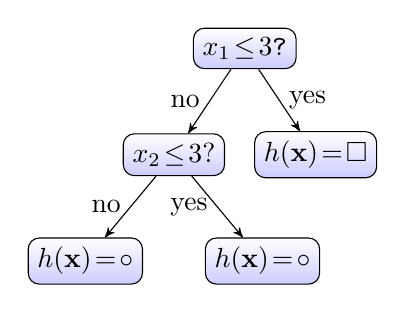
\begin{tikzpicture} [->,>=stealth',level/.style={sibling distance = 2cm/#1,
   level distance = 1.5cm},scale=0.9]
   \vspace*{-30mm} 
\tikzstyle{level 1}=[sibling distance=20mm]
  \tikzstyle{level 2}=[sibling distance=25mm]
\node [env] {$x_{1}\!\leq\!3$?}
child  {node [env] {$x_{2}\!\leq\!3?$} 
    child {node [env] {$h(\vx)\!=\!\circ$}  edge from parent node [left,align=center] {no}}
    child {node [env] {$h(\vx)\!=\!\circ$}   edge from parent node [left,align=center] {yes}}
  edge from parent node [left,align=center] {no} }
child { node [env]  {$h(\vx)\!=\!\Box$}
%   child {node [env] {$h(\vx)\!=\!y^{(1)}$}   edge from parent node [left,align=center] {no} }
  %  child {node [env] {$h(\vx)\!=\!y^{(4)}$}   edge from parent node [left,align=center] {yes} }
  edge from parent node [right,align=center] {yes}};
\end{tikzpicture}}
\end{minipage}
\hspace*{10mm}
\begin{minipage}{0.2\textwidth}
\scalebox{0.7}{
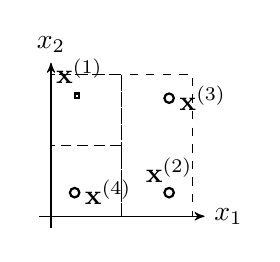
\begin{tikzpicture}[auto,scale=0.3]
%\draw [thick] (-3,-3) rectangle (1,4) node [anchor=east,above] {$\featurespace$} ;
\draw [thick] (5,5) circle (0.2cm)node[anchor=west] {\hspace*{0mm}$\vx^{(3)}$};
%\draw [dashed] (3,3) rectangle (6,6) ;
%\draw [dashed] (3,0) rectangle (6,3) ;
\draw [dashed] (3,0) rectangle (3,3) ;
\draw [dashed] (0,0) rectangle (3,6) ;
\draw [dashed] (0,0) rectangle (3,3) ;
\draw [dashed] (0,3) rectangle (3,6) ;
\draw [dashed] (3,0) rectangle (6,6) ;
\draw [thick] (1,1) circle (0.2cm)node[anchor=west] {\hspace*{0mm}$\vx^{(4)}$};
%\draw [thick] (-2,-1.7) circle (0.1cm)node[anchor=west] {\hspace*{0mm}$\vx^{(3)}$};
%\draw [thick] (2,-1.9) circle (0.1cm) node[anchor=west] {\hspace*{0mm}$\vx^{(2)}$};
\draw [thick] (5,1) circle (0.2cm)node[anchor=west,above] {\hspace*{0mm}$\vx^{(2)}$};
\draw [thick] (1,5) rectangle ++(0.2cm,0.2cm) node[anchor=west,above] {\hspace*{0mm}$\vx^{(1)}$};
\draw[->] (-0.5,0) -- (6.5,0) node[right] {$x_{1}$};
\draw[->] (0,-0.5) -- (0,6.5) node[above] {$x_{2}$};
%\foreach \y/\ytext in {0/0, 1/1,2/2,3/3,4/4,5/5,6/6} \draw[shift={(0,\y)}] (2pt,0pt) -- (-2pt,0pt) node[left] {$\ytext$};  
%\foreach \x/\xtext in{0/0, 1/1,2/2,3/3,4/4,5/5,6/6}\draw[shift={(\x,0)}] (0pt,2pt) -- (0pt,-2pt) node[below] {$\xtext$};  
\end{tikzpicture}}
\end{minipage}
\begin{minipage}{0.25\textwidth}
\scalebox{0.5}{
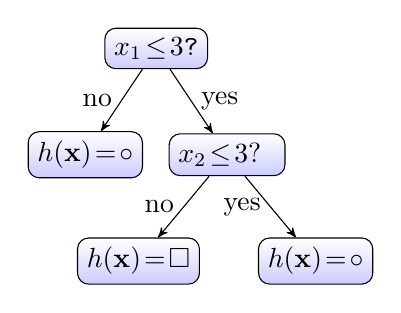
\begin{tikzpicture} [->,>=stealth',level/.style={sibling distance = 2cm/#1,
   level distance = 1.5cm},scale=0.9]
   \vspace*{-30mm} 
\tikzstyle{level 1}=[sibling distance=20mm]
  \tikzstyle{level 2}=[sibling distance=25mm]
\node [env] {$x_{1}\!\leq\!3$?}
child  {node [env] {$h(\vx)\!=\!\circ$} 
  edge from parent node [left,align=center] {no} }
child { node [env]  {$x_{2}\!\leq\!3?$ }
   child {node [env] {$h(\vx)\!=\!\Box$}   edge from parent node [left,align=center] {no} }
    child {node [env] {$h(\vx)\!=\!\circ$}   edge from parent node [left,align=center] {yes} }
  edge from parent node [right,align=center] {yes}};
\end{tikzpicture}}
\end{minipage}
\caption{Given the labeled dataset and a decision tree in the top row, 
	we grow the decision tree by expanding it at one of 
	its two leaf nodes. The bottom row shows two different 
	decision trees, along with their decision boundaries, 
	obtained by expanding different leaf nodes of the 
	tree in the top row.}
\label{fig_growingatree}
\end{figure}
 
One important aspect of learning decision trees from labeled 
data is the question of when to stop growing. A natural stopping 
criterion might be obtained from the limitations in computational 
resources, i.e., we can only afford to use decision trees up to 
certain maximum depth. Besides the computational limitations, 
we also face statistical limitations for the maximum size of decision 
trees. Very large decision trees, which represent 
highly complicated maps, we might end up overfitting the training 
data (see Figure \ref{fig_decisiontree_overfits} and Chapter \ref{ch_overfitting_regularization}) 
which is detrimental to the prediction performance of decision 
trees obtained for new data (which has not been used for training 
or growing the decision tree). 
 
 \section{ERM for Bayes' Classifiers} 
 \label{sec_ERM_Bayes} 
 
 The family of Bayes' classifiers is based on using the $0/1$ loss \eqref{equ_def_0_1} for 
 measuring the quality of a classifier $h$. The resulting ERM is 
 %Thus, in order to minimize the error probability, it is sensible to learn a good classifier $\hat{h}$ via ERM with $0/1$ loss: 
\begin{align}
\label{equ_approx_bayes_class}
\hat{h} & = \argmin_{h \in \hypospace} (1/\samplesize) \sum_{\sampleidx=1}^{\samplesize} \loss{(\vx^{(\sampleidx)},y^{(\sampleidx)})}{h}   \nonumber \\ 
                      & \stackrel{\eqref{equ_def_0_1}}{=}  \argmin_{h \in \hypospace} (1/\samplesize) \sum_{\sampleidx=1}^{\samplesize} \mathcal{I} ( h(\vx^{(\sampleidx)}) \neq y^{(\sampleidx)}). %\nonumber  \\
                 %     & \stackrel{\eqref{equ_0_1_approx_prob}}{\approx}\argmin_{h \in \hypospace} \prob{ h(\vx) \neq y} . 
\end{align}
The objective function in this optimization problem is non-differentiable 
and non-convex (see Figure \ref{fig_diff_types_bojec}). This prevents us 
from using gradient-based optimization methods (see Chapter \ref{ch_GD}) 
to solve \eqref{equ_approx_bayes_class}.

We will now approach the ERM \eqref{equ_approx_bayes_class} via a different 
route by interpreting the datapoints $(\vx^{(\sampleidx)},y^{(\sampleidx)})$ as 
realizations of i.i.d.\ random variables which are distributed according to some 
probability distribution $p(\vx,y)$. 

As discussed in Section \ref{sec_lossfct}, the empirical risk obtained using $0/1$ 
loss approximates the error probability $\prob { \hat{y} \neq y }$ with the predicted 
label $\hat{y} = 1$ for $h(\vx) > 0$ and $\hat{y} = -1$ otherwise (see \eqref{equ_0_1_approx_prob}). 
Thus, we can approximate the ERM \eqref{equ_approx_bayes_class} as 
\begin{align}
\label{equ_approx_bayes_class_approx}
\hat{h}    & \stackrel{\eqref{equ_0_1_approx_prob}}{\approx}\argmin_{h \in \hypospace} \prob{ \hat{y} \neq y} . 
\end{align}
Note that the hypothesis $h$, which is the optimization variable 
in \eqref{equ_approx_bayes_class_approx}, enters into the objective 
function of \eqref{equ_approx_bayes_class_approx} via the definition 
of the predicted label $\hat{y}$, which is $\hat{y} = 1 $ if $h(\vx) > 0$ 
and $\hat{y} =-1$ otherwise. 

%There are two challenges here: 
%\begin{itemize}
%\item First, we typically do not know the probability distribution which is underlying the training datapoints $(\vx^{(\sampleidx)},y^{(\sampleidx)})$ 
%and we therefore cannot evaluate the probability $\prob{ h(\vx) \neq y}$ for a given classifier $h \in \hypospace$. 
%\item Second, even if we are lucky and somehow have perfect knowledge of the underlying probability distribution and, in turn, 
%can compute $\prob{ h(\vx) \neq y}$, we would need to compute $\prob{ h(\vx) \neq y}$ for any possible classifier 
%$h \in \hypospace$ which is typically computationally intractable since the hypothesis space is too large. 
%\end{itemize}
It turns out that if we would know the probability distribution $p(\vx,y)$, which 
is required to compute $\prob{ \hat{y} \neq y}$, the solution of \eqref{equ_approx_bayes_class_approx} 
can be found easily via elementary Bayesian decision theory \cite{PoorDetEst}. In particular, 
the optimal classifier $h(\vx)$ is such that $\hat{y}$ achieves the maximum ``a-posteriori'' 
probability $p(\hat{y}|\vx)$ of the label being $\hat{y}$, given (or conditioned on) the features 
$\vx$. However, since we do not know the probability distribution $p(\vx,y)$, we have to estimate 
(or approximate) it from the observed datapoints $(\vx^{(\sampleidx)},y^{(\sampleidx)})$ which 
are modelled as i.i.d.\ random variables distributed according to $p(\vx,y)$. 

The estimation of $p(\vx,y)$ can be based on a particular probabilistic model for the features and 
labels which depends on certain parameters and then determining the parameters using maximum 
likelihood (see Section \ref{sec_max_iikelihood}). A widely used probabilistic model is based on 
Gaussian random vectors. In particular, conditioned on the label $y$, we model the feature vector 
$\vx$ as a Gaussian vector with mean ${\bm \mu}_{y}$ and covariance ${\bf \Sigma}$, i.e., 
\begin{equation}
\label{equ_prob_model_Bayes}
p(\vx|y) = \mathcal{N}(\vx;{\bm \mu}_{y},{\bf \Sigma}).\footnote{We use the shorthand $\mathcal{N}(\vx;{\bm \mu},{\bf \Sigma})$ to denote the 
probability density function $$p(\vx) = \frac{1}{\sqrt{{\rm det} (2 \pi {\bf \Sigma})}} \exp\big(- (1/2) (\vx\!-\!{\bm \mu})^{T}{\bf \Sigma}^{-1}(\vx\!-\!{\bm \mu}) \big)$$ of 
a Gaussian random vector $\vx$ with mean ${\bm \mu} = \expect \{ \vx \}$ and covariance matrix ${\bf \Sigma} = \expect \big\{(\vx\!-\!{\bm \mu})  (\vx\!-\!{\bm \mu})^{T} \big\}$.}
\end{equation} 

Given (conditioned on) the label $y$ of a data point, the conditional mean 
of the features  $\vx$ of this data point is ${\bm \mu}_{1}$ if $y=1$, while 
for $y=-1$ the conditional mean of $\vx$ is ${\bm \mu}_{-1}$. In contrast, the 
conditional covariance matrix ${\bf \Sigma} = \expect\{ (\vx-{\bm \mu}_{y})(\vx-{\bm \mu}_{y})^{T}|y \}$ 
of $\vx$ is the same for both values of the label $y \in \{-1,1\}$. 
The conditional probability distribution $p(\vx|y)$ of the feature vector, 
given the label $y$, is multivariate normal. In contrast, the marginal distribution 
of the features $\vx$ is a Gaussian mixture model (see Section \ref{sec_soft_clustering}).

%A ``naive'' Bayes' classifier is obtained by modelling the distribution of the features $\vx \in \mathbb{R}^{\featuredim}$, conditioned on the label $y \in \{-1,1\}$, 
%as a Gaussien random vector $\vx | y \sim \mathcal{N}({\bm \mu}_{y},{\bf \Sigma})$ with mean ${\bm \mu}_{y} \in \mathbb{R}^{\featuredim}$ and diagonal covariance 
%${\bf \Sigma} = {\rm diag} (\sigma_{1}^{2}, \ldots, \sigma_{\featuredim}^{2}) \in \mathbb{R}^{\featuredim \times \featuredim}$. 

For this probabilistic model of features and labels, the optimal classifier minimizing the 
error probability $\prob{\hat{y} \neq y}$ is $\hat{y}\!=\!1$ for $h(\vx)\!>\!0$ and $\hat{y}\!=\!-1$ 
for $h(\vx)\!\leq\!0$ using the classifier map 
\begin{equation}
\label{equ_classif_Bayes}
h(\vx) = \vw^{T} \vx \mbox{ with } \vw =  {\bf \Sigma}^{-1} ({\bm \mu}_{1} - {\bm \mu}_{-1}). 
\end{equation}
Carefully note that this expression is only valid if the matrix ${\bf \Sigma}$ is 
invertible.

We cannot implement the classifier \eqref{equ_classif_Bayes} directly, since we do not know the 
true values of the class-specific mean vectors ${\bm \mu}_{1}$, ${\bm \mu}_{-1}$ and covariance 
matrix ${\bf \Sigma}$. Therefore, we have to replace those unknown parameters with some 
estimates $\hat{\bm \mu}_{1}$, $\hat{\bm \mu}_{-1}$ and $\widehat{\bf \Sigma}$. A principled 
approach is to use the maximum likelihood estimates (see \eqref{equ_ML_mean_cov_Gauss}) 
\begin{align}
\hat{\bm \mu}_{1}  & = (1/\samplesize_{1}) \sum_{\sampleidx=1}^{\samplesize} \mathcal{I}(y^{(\sampleidx)}=1) \vx^{(\sampleidx)}, \nonumber \\
\hat{\bm \mu}_{-1}  & = (1/\samplesize_{-1}) \sum_{\sampleidx=1}^{\samplesize} \mathcal{I}(y^{(\sampleidx)}=-1) \vx^{(\sampleidx)}, \nonumber \\
\hat{\bm \mu} & =  (1/\samplesize) \sum_{\sampleidx=1}^{\samplesize} \vx^{(\sampleidx)}, \nonumber \\
 \mbox{and } \widehat{\bf \Sigma} & = (1/\samplesize) \sum_{\sampleidx=1}^{\samplesize} (\vz^{(\sampleidx)} - \hat{\bm \mu})(\vz^{(\sampleidx)} - \hat{\bm \mu})^{T}, \label{ML_est_naive_Bayes}
\end{align}
with $\samplesize_{1} = \sum_{\sampleidx=1}^{\samplesize}  \mathcal{I}(y^{(\sampleidx)}=1)$ 
denoting the number of datapoints with label $y=1$ ($\samplesize_{-1}$ is defined similarly). 
Inserting the estimates \eqref{ML_est_naive_Bayes} into \eqref{equ_classif_Bayes} yields the 
implementable classifier 
\begin{equation}
\label{equ_classif_Bayes_impl}
h(\vx) = \vw^{T} \vx \mbox{ with } \vw =  \widehat{\bf \Sigma}^{-1} (\hat{\bm \mu}_{1} - \hat{\bm \mu}_{-1}). 
\end{equation} 
We highlight that the classifier \eqref{equ_classif_Bayes_impl} is only well-defined if the estimated 
covariance matrix $\widehat{\bf \Sigma}$ \eqref{ML_est_naive_Bayes} is invertible. This requires 
to use a sufficiently large number of training datapoints such that $\samplesize \geq \featuredim$. 

We derived the classifier \eqref{equ_classif_Bayes_impl} as an approximate solution 
to the ERM \eqref{equ_approx_bayes_class}. The classifier \eqref{equ_classif_Bayes_impl} 
partitions the feature space $\mathbb{R}^{\featuredim}$ into two half-spaces. One 
half-space consists of feature vectors $\vx$ for which the hypothesis \eqref{equ_classif_Bayes_impl} 
is non-negative and, in turn, $\hat{y}=1$. The other half-space is constituted by feature 
vectors $\vx$ for which the hypothesis \eqref{equ_classif_Bayes_impl} is negative and, in turn, 
$\hat{y}=-1$. Figure \ref{fig_lin_dec_boundary} illustrates these two half-spaces and the 
decision boundary between them. 

The Bayes' classifier \eqref{equ_classif_Bayes_impl} is another instance of a linear 
classifier like logistic regression and the SVM. Each of these methods learns a 
linear hypothesis $h(\vx)=\vw^{T} \vx$, whose decision boundary (vectors $\vx$ with $h(\vx)=0$) 
is a hyperplane (see Figure \ref{fig_lin_dec_boundary}). However, these methods 
use different loss functions for assessing the quality of a particular linear hypothesis 
$h(\vx)=\vw \vx$ (which defined the decision boundary via $h(\vx)=0$). 
Therefore, these three methods typically learn classifiers with different decision 
boundaries. 

For the estimator $\widehat{\bf \Sigma}$ \eqref{equ_ML_mean_cov_Gauss} 
to be accurate (close to the unknown covariance matrix) we need a number 
of datapoints (sample size) which is at least of the order $\featuredim^{2}$. 
This sample size requirement might be infeasible for applications with only few 
datapoints available. 

The maximum likelihood estimate $\widehat{\bf \Sigma}$ \eqref{ML_est_naive_Bayes} 
is not invertible whenever $\samplesize < \featuredim$. In this case, the expression 
\eqref{equ_classif_Bayes_impl} becomes useless. To cope with small sample size 
$\samplesize < \featuredim$ we can simplify the model \eqref{equ_prob_model_Bayes} 
by requiring the covariance to be diagonal ${\bf \Sigma} = {\rm diag} (\sigma_{1}^{2}, \ldots, \sigma_{\featuredim}^{2})$. 
This is equivalent to modelling the individual features $x_{1},\ldots,x_{\featuredim}$ 
of a datapoint as conditionally independent, given its label $y$. The resulting special case of a Bayes' classifier is often referred to as a 
{\bf naive Bayes} classifier. 

We finally highlight that the classifier \eqref{equ_classif_Bayes_impl} 
is obtained using the generative model \eqref{equ_prob_model_Bayes} 
for the data. Therefore, Bayes' classifiers belong to the family of generative 
ML methods which involve modelling the data generation. In contrast, 
logistic regression and SVM do not require a generative model for the 
datapoints but aim directly at finding the relation between features $\vx$ 
and label $y$ of a datapoint. These methods belong therefore to the 
family of discriminative ML methods. 


Generative methods such as Bayes' classifier are preferable for 
applications with only very limited amounts of labeled data. Indeed, 
having a generative model such as \eqref{equ_prob_model_Bayes} 
allows to synthetically generate more labeled data by generating 
random features and labels according to the probability distribution 
\eqref{equ_prob_model_Bayes}. We refer to \cite{NIPS2001_2020} 
for a more detailed comparison between generative and discriminative 
methods. 




\section{Training and Inference Periods} 
\label{sec_training_inference} 

Some ML methods repeat the cycle in Figure \ref{fig_AlexMLBP} in a 
highly irregular fashion. Consider a large image collection which we 
use to learn a hypothesis about how cat images look like. It might 
be reasonable to adjust the hypothesis by fitting a model to the image 
collection. This fitting or training amounts to repeating the 
cycle in Figure \ref{fig_AlexMLBP} during some specific time period 
(the ``training time'') for a large number. 

After the training period, we only apply the hypothesis to predict 
the labels of new images. This second phase is also known 
as inference time and might be much longer compared to the 
training time. Ideally, we would like to only have a very short 
training period to learn a good hypothesis and then only use 
the hypothesis for inference. 

\section{Online Learning} 
\label{sec_online_learning}

So far we considered the training set to be an unordered set of datapoints 
whose labels are known. Many applications generate data in a sequential 
fashion, datapoints arrive incrementally over time. It is then desirable to update 
the current hypothesis as soon as new data arrives. 

ML methods differ in the frequency of iterating the cycle in Figure \ref{fig_AlexMLBP}. Consider a 
temperature sensor which delivers a new measurement every ten seconds. As soon as a new 
temperature measurement arrives, a ML method can use it to improve its hypothesis about 
how the temperature evolves over time. Such ML methods operate in an online fashion by 
continuously learning an improved model as new data arrives.  

To illustrate online learning, we consider the ML problem discussed in Section \ref{sec_putting_togehter_the_pieces}. 
This problem amounts to learning a linear predictor for the label $y$ of datapoints 
using a single numeric feature $x$. We learn the predictor based on some training 
data. The weight vector for the optimal linear predictor is characterized by \eqref{equ_zero_grad_condition_putting_together_special_form_mtx}. 

Let us assume that the training data is built up sequentially, we start with $m=1$ datapoints 
in the first time step, then in the next time step collect another datapoint to get 
$m=2$ datapoints, \ldots. We denote the feature matrix and label vector at time $m$ 
by $\mX^{(\samplesize)}$ and $\vy^{(\samplesize)}$: 
\begin{align}
m&=1: \quad &\mX^{(1)} & = \big( \vx^{(1)} \big)^{T}  \mbox{ , } & \vy^{(1)} & = \big( y^{(1)} \big)^{T} \mbox{, } \\ 
m&=2: \quad &\mX^{(2)} & = \big( \vx^{(1)},\vx^{(2)} \big)^{T}  \mbox{ , } & \vy^{(2)} & = \big( y^{(1)},y^{(2)} \big)^{T} \mbox{, } \\ 
m&=3: \quad &\mX^{(3)} & = \big( \vx^{(1)},\vx^{(2)},\vx^{(3)} \big)^{T}  \mbox{ , } & \vy^{(3} & = \big( y^{(1)},y^{(2)},y^{(3)} \big)^{T}.
\end{align} 
Note that in this online learning setting, the sample size $\samplesize$ has the meaning of a time index. 

Naively, we could try to solve the optimality condition \eqref{equ_zero_grad_condition_putting_together_special_form_mtx} 
for each time step $\samplesize$. However, this approach does not reuse computations already invested 
in solving \eqref{equ_zero_grad_condition_putting_together_special_form_mtx} at previous time steps $\samplesize' < \samplesize$. 





\section{Exercise} 
\label{sec_exercise_chap_4} 

\subsection{Uniqueness in Linear Regression}
\label{ex_chap_5_lin_reg} 
Consider linear regression with squared error loss. When 
is the optimal linear predictor unique. Does there always exist an optimal linear predictor?


\subsection{A Simple Linear Regression Method}
\label{ex_chap_5_bias}
Consider datapoints characterized by single numeric feature $x$ 
and label $y$. We learn a hypothesis map of the form $h(x) = x + b$ 
with some bias $b \in \mathbb{R}$. Can you write down a formula 
for the optimal $b$, that minimizes the average squared error on 
training data $\big(x^{(1)},y^{(1)} \big),\ldots,\big(x^{(\samplesize)},y^{(\samplesize)}\big)$.   
	
\subsection{A Simple Least Absolute Deviation Method}
\label{ex_chap_5_bias_absoluate_error}
Consider datapoints characterized by single numeric feature $x$ 
and label $y$. We learn a hypothesis map of the form $h(x) = x + b$ 
with some bias $b \in \mathbb{R}$. Can you write down a formula 
for the optimal $b$, that minimizes the average absolute error on 
training data $\big(x^{(1)},y^{(1)} \big),\ldots,\big(x^{(\samplesize)},y^{(\samplesize)}\big)$.   
		

\subsection{Polynomial Regression} 
\label{ex_chap_5_poly_reg} 
Polynomial regression for datapoints with a single feature $x$ and 
label $y$ is equivalent to linear regression with the feature 
vectors $\vx = \big(x^{0},x^{1},\ldots,x^{\featuredim-1}\big)^{T}$. 
Given $\samplesize = \featurelen$ datapoints $\big(x^{(1)},y^{(1)}\big),\ldots,\big(x^{(\samplesize)},y^{(\samplesize)}\big)$, 
we construct the feature matrix $\mathbf{X} \in \mathbb{R}^{\samplesize \times \samplesize}$. 
The columns of the feature matrix are the feature vectors $\vx^{(\sampleidx)}$. 
Is this feature matrix a Vandermonde matrix \cite{Gautschi1988}? Can you say 
something about the determinant of the feature matrix?

\subsection{Empirical Risk Approximates Expected Loss} 
\label{ex_chap_5_empriskapp} 
Consider training datapoints $\big(x^{(i)},y^{(i)} \big)$, for $\sampleidx = 1,\ldots,100$. 
The datapoints are i.i.d.\ realizations of a random datapoint $(x,y)$. 
The feature $x$ of a random datapoint is a Gaussian random variable 
with zero mean and unit variance. The label is modelled as 
via $y = x + e$ with noise $e \sim \mathcal{N}(0,1)$ being 
a standard Gaussian RV. The feature $x$ and noise $e$ 
are statistically independent. For the hypothesis $h(x)=0$, 
what is the probability that the empirical risk (average loss) on 
the training data is more than $20$ \% larger than the 
expected loss or risk? What is the expectation and variance 
of the training error and how are those related to the 
expected loss ? 





\newpage
\chapter{Gradient-Based Learning}
\label{ch_GD}

ML methods are optimization methods, that learn an optimal 
hypothesis out of the model. The quality of each hypothesis is 
measured or scored by some average loss or empirical risk. This
average loss, viewed as a function of the hypothesis, defines 
an objective function whose minimum is achieved by the 
optimal hypothesis. 

Many ML methods use gradient-based methods to efficiently search 
for a (nearly) optimal hypothesis. These methods locally 
approximate the objective function by a linear function which 
is used to improve the current guess for the optimal hypothesis. 
The prototype of a gradient-based optimization method is {\bf gradient descent} (GD). 

Variants of GD are used to tune the weights of artificial neural 
networks within deep learning methods \cite{Goodfellow-et-al-2016}. 
GD can also be applied to reinforcement learning applications. The 
difference between these applications is merely in the details for 
how to compute or estimate the gradient and how to incorporate 
the information provided by the gradients. 

In the following, we will mainly focus on ML problems with hypothesis 
space $\hypospace$ consisting of predictor maps $h^{(\vw)}$ 
which are parameterized by a weight vector $\vw \in \mathbb{R}^{\featuredim}$. 
Moreover, we will restrict ourselves to loss functions $\loss{(\vx,y)}{h^{(\vw)}}$ 
which depend smoothly on the weight vector $\vw$. 

Many important ML problems, including linear regression (see Section \ref{sec_lin_regression}) 
and logistic regression (see Section \ref{sec_LogReg}), involve in a smooth loss 
function. A smooth function $f: \mathbb{R}^{\featuredim} \rightarrow \mathbb{R}$ 
has continuous partial derivatives of all orders. In particular, we can define the 
gradient $\nabla f(\vw)$ for a smooth function $f(\vw)$ at every point $\vw$.

For a smooth loss function, the resulting ERM (see \eqref{eq_def_ERM_weight})  
\begin{align}
\label{equ_def_ERM_continous}
\vw_{\rm opt} & = \argmin_{\vw \in \mathbb{R}^{\featuredim}}  \emperror( h^{(\vw)} \mid \dataset)  \nonumber \\
& = \underbrace{(1/\samplesize) \sum_{\sampleidx=1}^{\samplesize} \loss{(\vx^{(\sampleidx)},y^{(\sampleidx)})}{h^{(\vw)}}}_{\defeq f(\vw)} 
\end{align} 
is a {\bf smooth optimization problem}
\begin{equation}
\label{equ_generic_smooth_problem}
\min_{\vw \in \mathbb{R}^{\featuredim}} f(\vw)
\end{equation} 
with a smooth function $f: \mathbb{R}^{\featuredim} \rightarrow \mathbb{R}$ of 
the vector argument $\vw \in \mathbb{R}^{\featuredim}$. 

We can approximate a smooth function $f(\vw$) locally around some point $\vw_{0}$ 
using a hyperplane. This hyperplane passes through the point $(\vw_{0},f(\vw_{0}))$ and 
has the normal vector $\mathbf{n} = (\nabla f(\vw_{0}),-1)$ (see Figure \ref{fig_smooth_function}). 
Elementary calculus yields the following linear approximation (around a point $\vw_{0}$) 
\cite{RudinBookPrinciplesMatheAnalysis}
\begin{equation} 
\label{equ_linear_approx_diff}
f(\vw) \approx f(\vw_{0}) + (\vw-\vw_{0})^{T} \nabla f(\vw_{0}) \mbox{ for }\vw \mbox{ sufficiently close to } \vw_{0}.
\end{equation}  

The approximation \eqref{equ_linear_approx_diff} lends naturally to an 
iterative method for finding the minimum of the function $f(\vw)$. This 
method is known as gradient descent (GD) and (variants of it) underlies 
many state-of-the-art ML methods, including deep learning methods. 

\begin{figure}[htbp]
\begin{center}
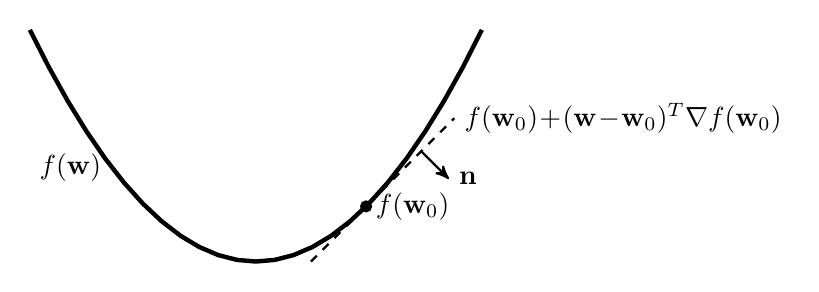
\begin{tikzpicture}[scale=0.7]
\node [right] at (-4.1,1.7) {$f(\vw)$} ;
\draw[ultra thick, domain=-4.1:4.1] plot (\x,  {(1/4)*\x*\x});
\draw[dashed, thick, domain=1:3.6] plot (\x,  {\x - 1}) node[right] {$ f(\vw_{0})\!+\!(\vw\!-\!\vw_{0})^{T} \nabla f(\vw_{0})$};
\draw [fill] (2,1) circle [radius=0.1] node[right] {$f(\vw_{0})$};
\draw[thick,->] (3,2) -- (3.5,1.5) node[right] {$\mathbf{n}$};
\end{tikzpicture}
\end{center}
\caption{A smooth function $f(\vw)$ can be approximated locally around 
	a point $\vw_{0}$ using a hyperplane whose normal vector 
	$\mathbf{n} = (\nabla f(\vw_{0}),-1)$ is determined by the 
	gradient $\nabla f(\vw_{0})$.}
\label{fig_smooth_function}
\end{figure}



\section{The Basic GD Step}
\label{sec_basic_GD_iteration}

We now discuss a very simple, yet quite powerful, algorithm for 
finding the weight vector $\vw_{\rm opt}$ which solves continuous 
optimization problems like \eqref{equ_def_ERM_continous}. 

Let us assume we have already some guess (or approximation) 
$\vw^{(k)}$ for the optimal weight vector $\vw_{\rm opt}$ and 
would like to improve it to a new guess $\vw^{(k+1)}$ which yields 
a smaller value of the objective function $f(\vw^{(k+1)}) < f(\vw^{(k)})$. 

For a differentiable objective function $f(\vw)$, we can use the 
approximation $f(\vw^{(k+1)})  \approx f(\vw^{(k)}) + (\vw^{(k+1)} - \vw^{(k)})^{T} \nabla f(\vw^{(k)})$ (cf. \eqref{equ_linear_approx_diff}) for $\vw^{(k+1)}$ not too far away from $\vw^{(k)}$. %(cf. \eqref{equ_linear_approx_diff}). 
Thus, we should be able to enforce $f(\vw^{(k+1)}) < f(\vw^{(k)})$ 
by choosing 
\begin{equation} 
\label{equ_def_GD_step}
\vw^{(k+1)} = \vw^{(k)} - \alpha \nabla f(\vw^{(k)})
\end{equation} 
with a sufficiently small {\bf step size} $\alpha>0$ (a small $\alpha$ 
ensures that the linear approximation \eqref{equ_linear_approx_diff} is valid). 
Then, we repeat this procedure to obtain $\vw^{(k+2)} = \vw^{(k+1)} - \alpha \nabla f(\vw^{(k+1)})$ and so on. 

The update \eqref{equ_def_GD_step} amounts to a {\bf gradient descent (GD) step}. 
For a convex differentiable objective function $f(\vw)$ 
and sufficiently small step size $\alpha$, the iterates $f(\vw^{(k)})$ 
obtained by repeating the GD steps \eqref{equ_def_GD_step} converge 
to a minimum, i.e., $\lim_{k \rightarrow \infty} f(\vw^{(k)}) = f(\vw_{\rm opt})$ (see Figure \ref{fig_basic_GD_step}). 

When the GD step is used within an ML method (see Section \ref{sec_lin_reg} 
and Section \ref{sec_LogReg}), the step size $\alpha$ is also referred to 
as the {\bf learning rate}. 
\begin{figure}
\begin{center}
  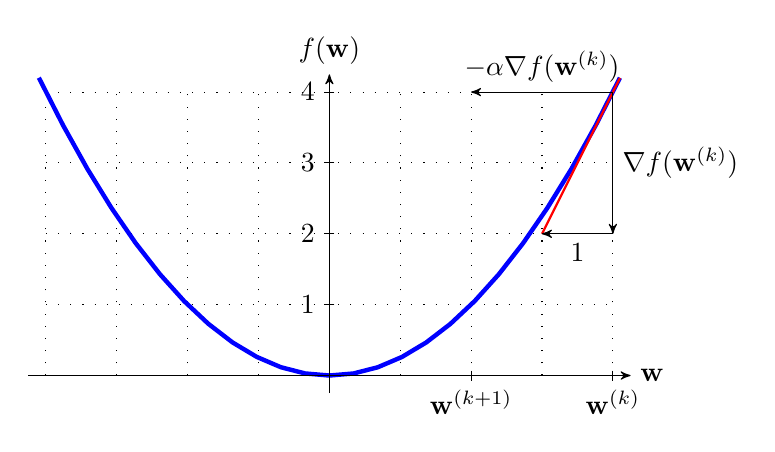
\begin{tikzpicture}[scale=0.9]
    \draw[loosely dotted] (-4,0) grid (4,4);
       \draw[blue, ultra thick, domain=-4.1:4.1] plot (\x,  {(1/4)*\x*\x});
             \draw[red, thick, domain=3:4.1] plot (\x,  {2*\x - 4});
                 \draw[->] (4,4) -- node[right] {$\nabla f(\vw^{(k)})$} (4,2);
                   \draw[->] (4,4) -- node[above] {$-\alpha \nabla f(\vw^{(k)})$} (2,4);
                   \draw[->] (4,2) -- node[below] {$1$} (3,2) ;
    \draw[->] (-4.25,0) -- (4.25,0) node[right] {$\vw$};
   \draw[->] (0,-0.25) -- (0,4.25) node[above] {$f(\vw)$};
    \draw[shift={(4,0)}] (0pt,2pt) -- (0pt,-2pt) node[below] {$\vw^{(k)}$};
    \draw[shift={(2,0)}] (0pt,2pt) -- (0pt,-2pt) node[below] {$\vw^{(k+1)}$};
    \foreach \y/\ytext in {1/1, 2/2, 3/3, 4/4}
    \draw[shift={(0,\y)}] (2pt,0pt) -- (-2pt,0pt) node[left] {$\ytext$};  
\end{tikzpicture}
\end{center}
\caption{The GD step \eqref{equ_def_GD_step} amounts to a shift by $-\alpha \nabla f(\vw^{(k)})$.}
\label{fig_basic_GD_step}
\end{figure}

In order to implement the GD step \eqref{equ_def_GD_step} we need 
to choose the step size $\alpha$ and we need to be able to compute 
the gradient $\nabla f(\vw^{(k)})$. Both tasks can be very challenging 
for an ML problem. 

The success of deep learning methods, which represent predictor maps 
using ANN (see Section \ref{sec_deep_learning}), can be partially attributed to 
the ability of computing the gradient $\nabla f(\vw^{(k)})$ efficiently 
via a message passing protocol known as {\bf back-propagation} \cite{Goodfellow-et-al-2016}. 

For the particular case of linear regression (see Section \ref{sec_lin_regression}) 
and logistic regression (see Section \ref{sec_GD_logistic_regression}), we 
will present precise conditions on the step size $\alpha$ which guarantee 
convergence of GD in Section \ref{sec_lin_reg} and Section \ref{sec_GD_logistic_regression}. 
Moreover, the objective functions $f(\vw)$ arising within linear and logistic 
regression allow for closed-form expressions of the gradient $\nabla f(\vw)$.

\section{Choosing Step Size} 

\begin{figure}[hbtp]
\begin{center}
\begin{minipage}{0.45\columnwidth}
  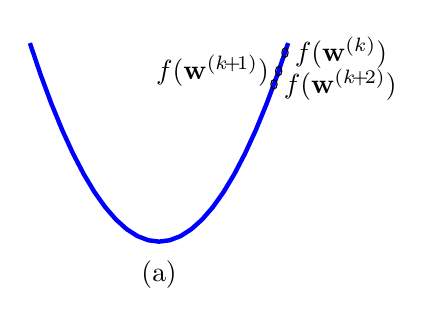
\begin{tikzpicture}[xscale=0.4,yscale=0.6]
 \draw[blue, ultra thick, domain=-4.1:4.1] plot (\x,  {(1/4)*\x*\x});
  \draw[] (4,4) circle [radius=0.1];
\node [right] at (4,4) {$f(\vw^{(k)})$};
      \draw[] (3.8,3.61) circle [radius=0.1];
\node [left] at (3.8,3.61) {$f(\vw^{(k\!+\!1)})$};
    \draw[] (3.65,3.33) circle [radius=0.1];
\node [right] at (3.65,3.33) {$f(\vw^{(k\!+\!2)})$};
    \node [below] at (0,-0.2) {(a)};
\end{tikzpicture}
\end{minipage}
\begin{minipage}{0.45\columnwidth}
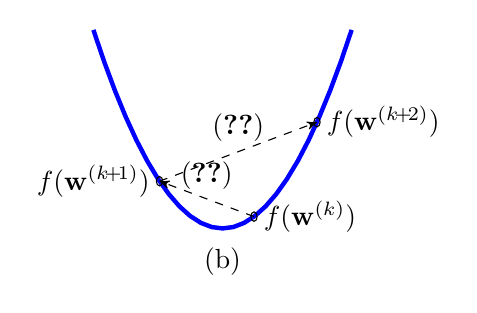
\begin{tikzpicture}[xscale=0.4,yscale=0.6]
\draw[blue, ultra thick, domain=-4.1:4.1] plot (\x,  {(1/4)*\x*\x});
\draw[] (1,0.25) circle [radius=0.1] node [right] (A) {$f(\vw^{(k)})$} ;
\draw[] (-2,1) circle [radius=0.1] node [left] (B) {$f(\vw^{(k\!+\!1)})$} ;
\draw[] (3,2.25) circle [radius=0.1]  node  [right] (C) {$f(\vw^{(k\!+\!2)})$} ;
\draw[->,dashed] (-2,1) -- (3,2.25) node [midway,above] {\eqref{equ_def_GD_step}};
\draw[->,dashed]  (1,0.25) -- (-2,1) node [midway,above] {\eqref{equ_def_GD_step}};
\node [below] at (0,-0.2) {(b)};
\end{tikzpicture}
\end{minipage}
\end{center}
\caption{Effect of choosing learning rate $\alpha$ in GD step 
	\eqref{equ_def_GD_step} too small (a) or too large (b). If the 
	steps size $\alpha$ in the GD step \eqref{equ_def_GD_step} is 
	chosen too small, the iterations make very little progress 
	towards the optimum or even fail to reach the optimum at all. 
	If the learning rate $\alpha$ is chosen too large, the iterates $\vw^{(\itercntr)}$ 
    might not converge at all (it might happen that $f(\vw^{(\itercntr\!+\!1)}) > f(\vw^{(\itercntr)})$!). }
\label{fig_small_large_alpha}
\end{figure}

The choice of the step size $\alpha$ in the GD step \eqref{equ_def_GD_step} 
has a strong impact on the performance of Algorithm \ref{alg:gd_linreg}. If we 
choose the step size $\alpha$ too large, the GD steps \eqref{equ_def_GD_step} 
diverge (see Figure \ref{fig_small_large_alpha}-(b)) and, in turn, 
Algorithm \ref{alg:gd_linreg} fails to deliver a satisfactory approximation of 
the optimal weight vector $\vw^{(\rm opt)}$ (see \eqref{equ_def_cost_linreg}). 

If we choose the step size $\alpha$ too small (see Figure \ref{fig_small_large_alpha}-(a)), 
the updates \eqref{equ_def_GD_step} make only very little progress towards 
approximating the optimal weight vector $\vw_{\rm opt}$. In applications that
require real-time processing of data streams, it is possible to repeat the GD 
steps only for a moderate number. If the GD step size is chosen too 
small, Algorithm \ref{alg:gd_linreg} will fail to deliver a good approximation 
of $\vw_{\rm opt}$ within an acceptable number of iterations (which translates 
to computation time). 

The optimal choice of the step size $\alpha$ of GD can be a challenging 
task and many sophisticated approaches have been proposed for its 
solution (see \cite[Chapter 8]{Goodfellow-et-al-2016}). We will restrict 
ourselves to a simple sufficient condition on the step size which guarantees 
convergence of the GD iterations $\vw^{(k)}$ for $k=1,2,\ldots$. 

If the objective function $f(\vw)$ is convex and smooth, the 
GD steps \eqref{equ_def_GD_step} converge to an optimum 
$\vw_{\rm opt}$ for any step size $\alpha$ satisfying \cite{nestrov04}
\begin{equation} 
\label{equ_GD_conv_guarantee}
\alpha \leq \frac{1}{\lambda_{\rm max} \big( \nabla^{2} f(\vw) \big) }\mbox{ for all } \vw \in \mathbb{R}^{\featuredim}. 
\end{equation} 
Here, we use the Hessian matrix $ \nabla^{2} f(\vw) \in \mathbb{R}^{\featuredim \times \featuredim}$ 
of a smooth function $f(\vw)$ whose entries are the second-order 
partial derivatives $\frac{\partial f(\vw)}{\partial w_{i} \partial w_{j}}$ 
of the function $f(\vw)$. It is important to note that \eqref{equ_GD_conv_guarantee} 
guarantees convergence for every possible initialization $\vw^{(0)}$ 
of the GD iterations. 

Note that while it might be computationally challenging to determine the maximum eigenvalue 
$\lambda_{\rm max} \big( \nabla^{2} f(\vw) \big)$ for arbitrary $\vw$, it might still be feasible to find an 
upper bound $U$ for the maximum eigenvalue. If we know an upper bound $U \geq \lambda_{\rm max} \big( \nabla^{2} f(\vw) \big)$ (valid for all $\vw \in \mathbb{R}^{\featuredim}$), 
the step size $\alpha =1/U$ still ensures convergence of the GD iteration.

\section{When To Stop} 
Fixed number of iteration (for this we might use convergence analysis of GD methods); 
use gradient as indicator for distance to optimum; monitor decrease in objective function; 
monitor decrease in validation error

\section{GD for Linear Regression} 
\label{sec_lin_reg}

We will now formulate a complete ML algorithm. This algorithm is based on 
applying GD to the linear regression problem discussed in Section \ref{sec_lin_regression}. 
This algorithm learns the weight vector 
for a linear hypothesis (see \eqref{equ_lin_hypospace}) 
\begin{equation} 
\label{equ_def_lin_pred_GD}
h^{(\vw)}(\vx) = \vw^{T} \vx.
\end{equation}
The weight vector is chosen to minimize average 
squared error loss \eqref{equ_squared_loss}
\begin{equation} 
\label{equ_def_cost_linreg}
%f(\vw_{\rm opt})= \min_{\vw \in \mathbb{R}^{\featuredim}} 
\emperror(h^{(\vw)}| \dataset) \stackrel{\eqref{eq_def_ERM_weight}}{=} (1/\samplesize) \sum_{\sampleidx=1}^{\samplesize} (y^{(\sampleidx)} - \vw^{T} \vx^{(\sampleidx)})^{2}, 
\end{equation}
incurred by the predictor $h^{(\vw)}(\vx)$ when applied to 
the labeled dataset $\dataset=\{ (\vx^{(\sampleidx)}, y^{(\sampleidx)}) \}_{\sampleidx=1}^{\samplesize}$. 
The optimal weight vector $\vw_{\rm opt}$ for \eqref{equ_def_lin_pred_GD} is 
characterized as
\begin{equation} 
\label{equ_smooth_problem_linreg}
\vw_{\rm opt} = \argmin_{\vw \in \mathbb{R}^{\featuredim}} f(\vw) \mbox{ with } f(\vw) = (1/\samplesize) \sum_{\sampleidx=1}^{\samplesize} (y^{(\sampleidx)} - \vw^{T} \vx^{(\sampleidx)})^{2}. 
\end{equation} 

The optimization problem \eqref{equ_smooth_problem_linreg} is an instance of the smooth 
optimization problem \eqref{equ_generic_smooth_problem}.  
We can therefore use GD \eqref{equ_def_GD_step} to solve \eqref{equ_smooth_problem_linreg}, 
to obtain the optimal weight vector $\vw_{\rm opt}$. To implement GD, we need to compute 
the gradient $\nabla f(\vw)$. 

The gradient of the objective function in \eqref{equ_smooth_problem_linreg} is given by 
\begin{equation}
\label{equ_gradient_linear_regression}
\nabla f(\vw) = -(2/\samplesize) \sum_{\sampleidx=1}^{\samplesize} (y^{(\sampleidx)} - \vw^{T} \vx^{(\sampleidx)}) \vx^{(\sampleidx)}.
\end{equation} 
By inserting \eqref{equ_gradient_linear_regression} into the basic GD iteration \eqref{equ_def_GD_step}, we obtain Algorithm \ref{alg:gd_linreg}. 
\begin{algorithm}[htbp]
\caption{``Linear Regression via GD''}\label{alg:gd_linreg}
\begin{algorithmic}[1]
\renewcommand{\algorithmicrequire}{\textbf{Input:}}
\renewcommand{\algorithmicensure}{\textbf{Output:}}
\Require   labeled dataset $\dataset=\{ (\vx^{(\sampleidx)}, y^{(\sampleidx)}) \}_{\sampleidx=1}^{\samplesize}$ containing feature vectors 
$\vx^{(\sampleidx)} \in \mathbb{R}^{\featuredim}$ and labels $y^{(\sampleidx)} \in \mathbb{R}$; GD step size $\alpha >0$. 
\Statex\hspace{-6mm}{\bf Initialize:} set $\vw^{(0)}\!\defeq\!\mathbf{0}$; set iteration counter $k\!\defeq\!0$   
\Repeat 
\State $k \defeq k +1$    (increase iteration counter) 
\State  $\vw^{(k)} \defeq \vw^{(k\!-\!1)} + \alpha (2/\samplesize) \sum_{\sampleidx=1}^{\samplesize} (y^{(\sampleidx)} - \big(\vw^{(k\!-\!1)})^{T} \vx^{(\sampleidx)}) \vx^{(\sampleidx)}$  (do a GD step \eqref{equ_def_GD_step})
\Until convergence 
\Ensure $\vw^{(k)}$ (which approximates $\vw_{\rm opt}$ in \eqref{equ_smooth_problem_linreg})
\end{algorithmic}
\end{algorithm}

Let us have a closer look on the update in step $3$ of Algorithm \ref{alg:gd_linreg}, which is 
\begin{equation}
\label{equ_update_gd_linreg}
\vw^{(k)} \defeq \vw^{(k\!-\!1)} + \alpha (2/\samplesize) \sum_{\sampleidx=1}^{\samplesize} (y^{(\sampleidx)} - \big(\vw^{(k\!-\!1)})^{T} \vx^{(\sampleidx)})\vx^{(\sampleidx)}. 
\end{equation}
The update \eqref{equ_update_gd_linreg} has an appealing form as it amounts to correcting the previous guess (or approximation) $\vw^{(k\!-\!1)}$ for 
the optimal weight vector $\vw_{\rm opt}$ by the correction term 
\begin{equation}
\label{equ_corr_term_linreg}
 (2\alpha/\samplesize) \sum_{\sampleidx=1}^{\samplesize} \underbrace{(y^{(\sampleidx)} - \big(\vw^{(k\!-\!1)})^{T} \vx^{(\sampleidx)})}_{e^{(\sampleidx)}} \vx^{(\sampleidx)}. 
\end{equation}
The correction term \eqref{equ_corr_term_linreg} is a weighted average of the feature vectors $\vx^{(\sampleidx)}$ using weights $(2\alpha/\samplesize) \cdot e^{(i)}$. 
These weights consist of the global factor $(2\alpha/\samplesize)$ (that applies equally to all feature vectors $\vx^{(\sampleidx)}$) and a sample-specific factor 
$e^{(\sampleidx)} = (y^{(\sampleidx)} - \big(\vw^{(k\!-\!1)})^{T} \vx^{(\sampleidx)})$, which is the prediction (approximation) error obtained by the linear predictor 
$h^{(\vw^{(k-1)})}(\vx^{(\sampleidx)}) =   \big(\vw^{(k\!-\!1)})^{T} \vx^{(\sampleidx)}$ when predicting the label $y^{(\sampleidx)}$ from the features $\vx^{(\sampleidx)}$. 

\begin{center}
\framebox[0.96\textwidth]{
 \parbox{0.9\textwidth}{
We can interpret the GD step \eqref{equ_update_gd_linreg} as an instance of ``learning by trial and error''. Indeed, 
the GD step amounts to ``trying out'' the predictor $h(\vx^{(\sampleidx)}) = \big(\vw^{(k\!-\!1)})^{T}\vx^{(\sampleidx)}$ and then correcting the weight vector $\vw^{(k\!-\!1)}$ 
according to the error $e^{(\sampleidx)} = y^{(\sampleidx)} - \big(\vw^{(k\!-\!1)})^{T} \vx^{(\sampleidx)}$. 
}}
\end{center}

%{\bf Exercise.} Consider the dataset with feature vectors $\vx^{(1)}=(100,0)^{T} \in \mathbb{R}^{2}$ and $\vx^{(2)} = (0,1/10)^{T}$ which we 
%stack into the matrix $\mX = (\vx^{(1)},\vx^{(2)})$. What is the condition number of $\mX \mX^{T}$? What is the condition number of $\widehat{\mathbf{X}}..$ 
%obtained from the normalized feature vectors $\hat{\vx}^{(\sampleidx)}$. 


The choice of the step size $\alpha$ used for Algorithm \ref{alg:gd_linreg} can be based on the sufficient condition \eqref{equ_GD_conv_guarantee} 
with the Hessian $\nabla^{2} f(\vw)$ of the objective function $f(\vw)$ underlying linear regression (see \eqref{equ_smooth_problem_linreg}). This 
Hessian is given explicitly as  
\begin{equation}
\label{equ_hessian_linreg}
\nabla^{2} f(\vw) = (1/\samplesize) \mX^{T} \mX, 
\end{equation}
with the feature matrix $\mX=\big(\vx^{(1)},\ldots,\vx^{(\samplesize)}\big)^{T} \in \mathbb{R}^{\samplesize \times \featuredim}$ (see \eqref{equ_def_vec_matrix}). 
Note that the Hessian \eqref{equ_hessian_linreg} does not depend on the weight vector $\vw$. 


Comparing \eqref{equ_hessian_linreg} with \eqref{equ_GD_conv_guarantee}, one particular strategy for choosing 
the step size in Algorithm \ref{alg:gd_linreg} is to (i) compute the matrix product $ \mX^{T} \mX$, (ii) compute the 
maximum eigenvalue $\lambda_{\rm max} \big(  (1/\samplesize)  \mX^{T} \mX \big)$ of this product and (iii) set 
the step size to $\alpha =1/\lambda_{\rm max} \big(  (1/\samplesize)  \mX^{T} \mX \big)$. 

While it might be challenging to compute the maximum eigenvalue $\lambda_{\rm max} \big(  (1/\samplesize)  \mX^{T} \mX \big)$, 
it might be easier to find an upper bound $U$ for it.\footnote{The problem of 
computing a full eigenvalue decomposition of $\mX^{T} \mX$ has essentially the same complexity as solving the 
ERM problem directly via \eqref{equ_zero_gradient_lin_reg}, which we want to avoid by using the ``cheaper'' GD algorithm.}
Given such an upper bound $U \geq \lambda_{\rm max} \big( (1/\samplesize)  \mX^{T} \mX \big)$, the step 
size $\alpha =1/U$ still ensures convergence of the GD iteration. Consider a dataset $\{(\vx^{(\sampleidx)},y^{(\sampleidx)})\}_{\sampleidx=1}^{\samplesize}$ 
with normalized features, i.e., $\| \vx^{(\sampleidx)}\| = 1$ for all $\sampleidx =1,\ldots,\samplesize$. Then, 
by elementary linear algebra, one can verify the upper bound $U= 1$, i.e., $ 1 \geq  \lambda_{\rm max} \big(  (1/\samplesize)  \mX^{T} \mX \big)$. 
We can then ensure convergence of the GD iterations $\vw^{(k)}$ (see \eqref{equ_update_gd_linreg}) by 
choosing the step size $\alpha =1$.

%\subsection{GD for Polynomial Regression} 
%\label{sec_poly_reg}
%??? Discuss how GD for Polynomial Regression does implicit regularisation (cf ``Early Stopping''). This has been discussed in {\rm https://www.youtube.com/watch?v=MG35HdwgFoY}. ????

\section{GD for Logistic Regression}
\label{sec_GD_logistic_regression}

%We can now formulate a full-fledged ML algorithm for solving a linear regression problem (see Section \ref{sec_lin_regression}). 
As discussed in Section \ref{sec_LogReg}, logistic regression learns 
a linear hypothesis $h^{(\vw_{\rm opt})}$ by minimizing the average 
logistic loss \eqref{equ_def_emp_risk_logreg} obtained for a dataset $\dataset= \{ (\vx^{(\sampleidx)}, y^{(\sampleidx)}) \}_{\sampleidx=1}^{\samplesize}$, with features $\vx^{(\sampleidx)} \in \mathbb{R}^{\featuredim}$ and binary labels 
$y^{(\sampleidx)} \in \{-1,1\}$. This minimization problem is an instance 
of the smooth optimization problem \eqref{equ_generic_smooth_problem},
\begin{align} 
\label{equ_smooth_problem_logeg}
\vw_{\rm opt} & = \argmin_{\vw \in \mathbb{R}^{\featuredim}} f(\vw) \nonumber \\ 
 \mbox{ with } f(\vw) & = (1/\samplesize) \sum_{\sampleidx=1}^{\samplesize} \log( 1\!+\!\exp ( - y^{(\sampleidx)} \vw^{T} \vx^{(\sampleidx)})). 
\end{align} 

To apply GD \eqref{equ_def_GD_step} to solve \eqref{equ_smooth_problem_logeg}, 
we need to compute the gradient $\nabla f(\vw)$. 
The gradient of the objective function in \eqref{equ_smooth_problem_logeg} is given by 
\begin{equation}
\label{equ_gradient_logistic_regression}
\nabla f(\vw) = (1/\samplesize) \sum_{\sampleidx=1}^{\samplesize} \frac{-y^{(\sampleidx)}}{1 + \exp ( y^{(\sampleidx)} \vw^{T} \vx^{(\sampleidx)})} \vx^{(\sampleidx)}.
\end{equation} 
By inserting \eqref{equ_gradient_logistic_regression} into the basic GD iteration \eqref{equ_def_GD_step}, we obtain Algorithm \ref{alg:gd_logreg}. 
\begin{algorithm}[htbp]
\caption{``Logistic Regression via GD''}\label{alg:gd_logreg}
\begin{algorithmic}[1]
\renewcommand{\algorithmicrequire}{\textbf{Input:}}
\renewcommand{\algorithmicensure}{\textbf{Output:}}
\Require   labeled dataset $\dataset=\{ (\vx^{(\sampleidx)}, y^{(\sampleidx)}) \}_{\sampleidx=1}^{\samplesize}$ containing feature vectors 
$\vx^{(\sampleidx)} \in \mathbb{R}^{\featuredim}$ and labels $y^{(\sampleidx)} \in \mathbb{R}$; GD step size $\alpha >0$. 
\Statex\hspace{-6mm}{\bf Initialize:}set $\vw^{(0)}\!\defeq\!\mathbf{0}$; set iteration counter $\itercntr\!\defeq\!0$   
\Repeat 
\State $\itercntr\!\defeq\! \itercntr\!+\!1$    (increase iteration counter) 
\State  $\vw^{(\itercntr)} \defeq \vw^{(\itercntr\!-\!1)}\!+\!\alpha (1/\samplesize) \sum_{\sampleidx=1}^{\samplesize} \frac{y^{(\sampleidx)}}{1\!+\!\exp \big( y^{(\sampleidx)} \big(\vw^{(\itercntr\!-\!1)}\big)^{T} \vx^{(\sampleidx)}\big)} \vx^{(\sampleidx)}$  (do a GD step \eqref{equ_def_GD_step})
\Until convergence 
\Ensure $\vw^{(\itercntr)}$, which approximates a solution $\vw_{\rm opt}$ of \eqref{equ_smooth_problem_logeg})
\end{algorithmic}
\end{algorithm}

Let us have a closer look on the update in step $3$ of Algorithm \ref{alg:gd_logreg}, which is 
\begin{equation}
\label{equ_update_logreg_GD}
\vw^{(k)} \defeq \vw^{(k\!-\!1)} + \alpha (1/\samplesize) \sum_{\sampleidx=1}^{\samplesize} \frac{y^{(\sampleidx)}}{1 + \exp \big( y^{(\sampleidx)} \big( \vw^{(k\!-\!1)}  \big)^{T} \vx^{(\sampleidx)}\big)} \vx^{(\sampleidx)}. 
\end{equation}
The update \eqref{equ_update_logreg_GD} has an appealing form as it amounts to correcting the previous 
guess (or approximation) $\vw^{(k\!-\!1)}$ for the optimal weight vector $\vw_{\rm opt}$ by the correction term 
\begin{equation}
\label{equ_correction_logreg_GD}
(\alpha/\samplesize) \sum_{\sampleidx=1}^{\samplesize} \underbrace{ \frac{y^{(\sampleidx)}}{1 + \exp ( y^{(\sampleidx)} \vw^{T} \vx^{(\sampleidx)})}}_{e^{(\sampleidx)}} \vx^{(\sampleidx)}. 
\end{equation}
The correction term \eqref{equ_correction_logreg_GD} is a weighted average 
of the feature vectors $\vx^{(\sampleidx)}$, each of which is weighted by the 
factor $(\alpha/\samplesize) \cdot e^{(i)}$. These weighting factors are a product 
of the global factor $(\alpha/\samplesize)$ that applies equally to all feature vectors 
$\vx^{(\sampleidx)}$. The global factor is multiplied by a datapoint-specific factor 
$e^{(\sampleidx)} =  \frac{y^{(\sampleidx)}}{1 + \exp ( y^{(\sampleidx)} \vw^{T} \vx^{(\sampleidx)})}$, 
which quantifies the error of the classifier  $h^{(\vw^{(k-1)})}(\vx^{(\sampleidx)}) =   \big(\vw^{(k\!-\!1)})^{T} \vx^{(\sampleidx)}$ 
for a single datapoint with true label $y^{(\sampleidx)} \in \{-1,1\}$ and features $\vx^{(\sampleidx)} \in \mathbb{R}^{\featuredim}$. 

We can use the sufficient condition \eqref{equ_GD_conv_guarantee} for the convergence of GD 
to guide the choice of the step size $\alpha$ in Algorithm \ref{alg:gd_logreg}. To apply condition 
\eqref{equ_GD_conv_guarantee}, we need to determine the Hessian $\nabla^{2} f(\vw)$ matrix of the 
objective function $f(\vw)$ underlying logistic regression (see \eqref{equ_smooth_problem_logeg}). 
Some basic calculus reveals (see \cite[Ch. 4.4.]{hastie01statisticallearning})
\begin{equation}
\label{equ_hessian_logreg}
\nabla^{2} f(\vw) =  (1/\samplesize) \mX^{T} \mD \mX. 
\end{equation}
Here, we used the feature matrix $\mX=\big(\vx^{(1)},\ldots,\vx^{(\samplesize)}\big)^{T} \in \mathbb{R}^{\samplesize \times \featuredim}$ (see \eqref{equ_def_vec_matrix}) 
and the diagonal matrix $\mD = {\rm diag} \{d_{1},\ldots,d_{\samplesize}\} \in \mathbb{R}^{\samplesize \times \samplesize}$ with diagonal elements 
\begin{equation}
d_{\sampleidx} = \frac{1}{1+\exp(-\vw^{T} \vx^{(\sampleidx)})} \bigg(1- \frac{1}{1+\exp(-\vw^{T} \vx^{(\sampleidx)})}  \bigg). \label{equ_diag_entries_log_reg}   % \frac{1}{1+\exp(-\vw^{T} \vx)} %\big( 1- \frac{1}{1+\exp(-\vw^{T} \vx)}  \big). 
\end{equation} 
We highlight that, in contrast to the Hessian \eqref{equ_hessian_linreg} obtained for the objective function 
arising in linear regression, the Hessian \eqref{equ_hessian_logreg} varies with the weight vector $\vw$. 
This makes the analysis of Algorithm \ref{alg:gd_logreg} and the optimal choice of step size somewhat 
more difficult compared to Algorithm \ref{alg:gd_linreg}. However, since the diagonal entries \eqref{equ_diag_entries_log_reg} 
take values in the interval $[0,1]$, for normalized features (with $\| \vx^{(\sampleidx)} \|=1$) the step size $\alpha=1$ 
ensures convergence of the GD updates \eqref{equ_update_logreg_GD} to the optimal weight vector 
$\vw_{\rm opt}$ solving \eqref{equ_smooth_problem_logeg}. 

\section{Data Normalization} 

The convergence speed of the GD steps \eqref{equ_def_GD_step}, i.e., the 
number of steps required to reach the minimum of the objective function 
\eqref{equ_def_cost_MSE} within a prescribed accuracy, depends crucially 
on the condition number $\kappa( \mX^{T} \mX)$. This condition number is 
defined as the ratio 
\begin{equation}
\label{equ_def_condition_number} 
\kappa( \mX^{T} \mX) \defeq \lambda_{\rm max}/\lambda_{\rm min}
\end{equation} 
between the largest and smallest eigenvalue of the matrix $\mX^{T} \mX$. 

The condition number is only well defined if the columns of the feature matrix $\mX$ 
(see \eqref{equ_def_vec_matrix}), which are precisely the feature vectors $\vx^{(\sampleidx)}$, 
are linearly independent. In this case the condition number is lower bounded 
as $\kappa( \mX^{T} \mX) \geq 1$. 

It can be shown that the GD steps \eqref{equ_def_GD_step} converge faster for 
smaller condition number $\kappa( \mX^{T} \mX)$ \cite{JungFixedPoint}. Thus, GD 
will be faster for datasets with a feature matrix $\mX$ such that  $\kappa( \mX^{T} \mX) \approx 1$. 
It is therefore often beneficial to pre-process the feature vectors using a {\bf normalization} 
(or {\bf standardization}) procedure as detailed in Algorithm \ref{alg_reshaping}. 
 
 \begin{algorithm}[htbp]
\caption{``Data Normalization''}\label{alg_reshaping}
\begin{algorithmic}[1]
\renewcommand{\algorithmicrequire}{\textbf{Input:}}
\renewcommand{\algorithmicensure}{\textbf{Output:}}
\Require   labeled dataset $\dataset = \{(\vx^{(\sampleidx)},y^{(\sampleidx)})\}_{\sampleidx=1}^{\samplesize}$
%\Statex\hspace{-6mm}{\bf Initialize:}set $\vw^{(0)}\!\defeq\!\mathbf{0}$; set iteration counter $k\!\defeq\!0$   
%\Repeat 
\vspace*{2mm}
\State remove sample means $\bar{\vx}=(1/\samplesize) \sum_{\sampleidx=1}^{\samplesize}  \vx^{(\timeidx)}$ from features, i.e., 
 \begin{equation}
 \nonumber
 \vx^{(\sampleidx)} \defeq \vx^{(\sampleidx)} - \bar{\vx} \mbox{ for  }  \sampleidx=1,\ldots,\samplesize
 \end{equation} 
\State normalise features to have unit variance,  
 \begin{equation} 
 \nonumber
 \hat{x}^{(\sampleidx)}_{j} \defeq x^{(\sampleidx)}_{j}/ \hat{\sigma}   \mbox{ for  } j=1,\ldots,\featuredim \mbox{ and } \sampleidx=1,\ldots,\samplesize
 \end{equation}
 with the empirical variance $\hat{\sigma}_{j}^{2}  =(1/\samplesize) \sum_{\sampleidx=1}^{\samplesize} \big( x^{(\sampleidx)}_{j} \big)^{2}$ 
\Ensure normalized feature vectors $\{\hat{\vx}^{(\sampleidx)}\}_{\sampleidx=1}^{\samplesize}$
\end{algorithmic}
\end{algorithm}
The preprocessing implemented in Algorithm \ref{alg_reshaping} reshapes (transforms) the 
original feature vectors $\vx^{(\sampleidx)}$ into new feature vectors $\hat{\vx}^{(\sampleidx)}$ 
such that the new feature matrix $\widehat{\mX} = (\hat{\vx}^{(1)},\ldots,\hat{\vx}^{(\samplesize)})^{T}$ 
tends to be well-conditioned, i.e., $\kappa( \widehat{\mX}^{T} \widehat{\mX}) \approx 1$. 

\begin{center}
\framebox[0.96\textwidth]{
 \parbox{0.9\textwidth}{
{\bf Exercise.} Consider the dataset with feature vectors $\vx^{(1)}=(100,0)^{T} \in \mathbb{R}^{2}$ 
and $\vx^{(2)} = (0,1/10)^{T}$ which we stack into the matrix $\mX = (\vx^{(1)},\vx^{(2)})^{T}$. 
What is the condition number of $\mX^{T} \mX$? What is the condition number of 
$\big(\widehat{\mX}\big)^{T} \widehat{\mX}$ with the matrix $\widehat{\mX}=(\hat{\vx}^{(1)},\hat{\vx}^{(2)})^{T}$ 
constructed from the normalized feature vectors $\hat{\vx}^{(\sampleidx)}$ delivered by Algorithm \ref{alg_reshaping}. 
}}
\end{center}
 
 
\section{Stochastic GD}

Consider an ML problem with a hypothesis space $\hypospace$ which is parametreized by a 
weight vector $\vw \in \mathbb{R}^{\featuredim}$ (such that each element $h^{(\vw)}$ of $\hypospace$ 
corresponds to a particular choice of $\vw$) and a loss function $\loss{(\vx,y)}{h^{(\vw)}}$ which 
depends smoothly on the weight vector $\vw$. The resulting ERM \eqref{equ_def_ERM_continous} 
amounts to a smooth optimization problem which can be solved using GD \eqref{equ_def_GD_step}. 

The gradient $\nabla f(\vw)$ obtained for the optimization problem 
\eqref{equ_def_ERM_continous} has a particular structure. Indeed, the 
gradient is a sum 
\vspace*{-2mm}
\begin{equation}
\label{eq_gradient_sum}
\nabla f(\vw) = (1/\samplesize) \sum_{\sampleidx=1}^{\samplesize} \nabla f_{\sampleidx}(\vw)   \mbox{ with } f_{\sampleidx}(\vw) \defeq \loss{(\vx^{(\sampleidx)},y^{(\sampleidx)})}{h^{(\vw)}}, 
\end{equation} 
with the components corresponding to the datapoints $(\vx^{(\sampleidx)},y^{(\sampleidx)})$, for $\sampleidx=1,\ldots,\samplesize$. 
Note that each GD step \eqref{equ_def_GD_step} requires to compute the gradient \eqref{eq_gradient_sum}. 

Computing the sum in \eqref{eq_gradient_sum} can be computationally challenging for at least 
two reasons. First, computing the sum exactly is challenging for extremely large datasets with 
$\samplesize$ in the order of billions. Second, for datasets which are stored in different data 
centres located all over the world, the summation would require a huge amount of 
network resources. Moreover, the finite transmission rate of communication networks 
limits the rate by which the GD steps \eqref{equ_def_GD_step} can be executed. 
\begin{center}
\framebox[0.96\textwidth]{
 \parbox{0.9\textwidth}{
{\bf ImageNet.} The ``ImageNet'' database contains more than $10^{6}$ images \cite{ImageNet}. These 
images are labeled according to their content (e.g., does the image show a dog?). Let us assume that 
each image is represented by a (rather small) feature vector $\vx \in \mathbb{R}^{\featuredim}$ 
of length $\featuredim=1000$. Then, if we represent each feature by a  floating point number, 
performing only one single GD update \eqref{equ_def_GD_step} per second would require at 
least $10^{9}$ FLOPS. 
}}
\end{center}


The idea of {\bf stochastic GD (SGD)} is to replace the exact gradient $\nabla f(\vw)$ 
by some approximation which can be computed easier than \eqref{eq_gradient_sum}. 
The word ``stochastic'' in the name SGD hints already at the use of stochastic approximations. 

A basic variant of SGD approximates the gradient $\nabla f(\vw)$ (see \eqref{eq_gradient_sum}) 
a randomly selected component $\nabla f_{\hat{\sampleidx}}(\vw)$ in \eqref{eq_gradient_sum}, 
with the index $\hat{\sampleidx}$ being chosen randomly out of $\{1,\ldots,\samplesize\}$. SGD 
amounts to iterating the update 
\begin{equation}
\label{equ_SGD_update}
\mathbf{w}^{(\itercntr+1)} = \mathbf{w}^{(\itercntr)} - \alpha \nabla f_{\hat{\sampleidx}}(\vw^{(\itercntr)}).
\end{equation} 
It is important to use a fresh randomly chosen index $\hat{i}$ during each new iteration. 
The indices used in different iterations are statistically independent. 

Note that SGD replaces the summation over all training datapoints in the GD step 
\eqref{equ_def_GD_step} just by the random selection of a single component of the sum. 
The resulting savings in computational complexity can be significant in applications 
where a large number of  datapoints is stored in a distributed fashion. However, this 
saving in computational complexity comes at the cost of introducing a non-zero 
gradient noise 
\begin{equation}
\label{equ_gradient_noise}
\varepsilon = \nabla f(\vw)  - \nabla f_{\hat{\sampleidx}}(\vw), 
\end{equation} 
into the SGD updates. 

To avoid a detrimental accumulation of the gradient noise \eqref{equ_gradient_noise} 
during the SGD updates \eqref{equ_SGD_update}, the step size $\alpha$ needs to be gradually 
decreased. Thus, the step-size used in the SGD update \eqref{equ_gradient_noise}
typically depends on the iteration number $\itercntr$, $\alpha\!=\!\alpha_{\itercntr}$. 
The sequence $\alpha_{\itercntr}$ of step-sizes is referred to as a {\bf learning rate schedule} \cite[Chapter 8]{Goodfellow-et-al-2016}. 
One popular choice for the learning rate schedule is $\alpha\!=\!1/\itercntr$ \cite{Murata98astatistical}. 
We consider conditions on the learning rate schedule that guarantee convergence of 
SGD in Exercise \ref{ex_SGD_learning_rate}. 

The SGD iteration \eqref{equ_SGD_update} assumes that the training data is already 
collected but so large that the sum in \eqref{eq_gradient_sum} is computationally intractable. 
Another variant of SGD is obtained by assuming a different data generation 
mechanism. If datapoints are collected sequentially, one new datapoint $\vx^{(\timeidx)},y^{(\timeidx)}$ 
at each new time step $\timeidx$, we could use a SGD variant for online learning 
(see Section \ref{sec_online_learning}). This online SGD algorithm amounts to 
computing, for each time step $\timeidx$, the iteration 
\begin{equation}
\label{equ_SGD_update_timeiedx}
\mathbf{w}^{(\timeidx+1)} = \mathbf{w}^{(\timeidx)} - \alpha_{\timeidx} \nabla f_{\timeidx+1}(\vw^{(\timeidx)}).
\end{equation} 



\section{Exercises}

\subsection{Use Knowledge About Problem Class} 
Consider the space $\mathcal{P}$ of sequences $f = (f[0],f[1],\ldots)$ 
that have the following properties 
\begin{itemize} 
	\item they are monotone increasing, $f[\itercntr'] \geq f[\itercntr]$ for any $\itercntr' \geq \itercntr$ and $f \in \mathcal{P}$
	\item a change point $\itercntr$, where $f[\itercntr] \neq f[\itercntr\!+\!1]$ can only be at integer multiples of $100$, 
	e.g., $\itercntr\!=\!100$ or $\itercntr\!=\!300$. 
\end{itemize} 
Given some unknown function $f \in \mathcal{P}$ and starting 
point $\itercntr_{0}$ the problem is to find the minimum value of $f$ as 
quickly as possible. We consider iterative algorithms that can query
the function at some point $\itercntr$ to obtain the values $f[\itercntr], f[\itercntr\!-\!1]$ and $f[\itercntr\!+\!1]$. 

\subsection{SGD Learning Rate Schedule} 
\label{ex_SGD_learning_rate}
Consider learning a linear hypothesis $h(\vx) = \vw^{T} \vx$ from datapoints 
that arrive sequentially. In each time step $\itercntr\!=\!1,\ldots,$, we collect 
a new datapoint $\big(\vx^{(\itercntr)},y^{(\itercntr)} \big)$. The 
datapoints are modelled as realizations of i.i.d.\ copies of a random data point $\big(\vx,y\big)$. 
The probability distribution of the features $\vx$ is a standard 
multivariate normal distribution $\mathcal{N}(\mathbf{0},\mathbf{I})$. 
The label of a random datapoint is related to its features via $y = \bar{\vw}^{T} \vx+ \varepsilon$ with 
standard Gaussian noise $ \varepsilon \sim \mathcal{N}(0,1)$. 
We use SGD to learn the weight vector $\vw$ of a linear hypothesis, 
\begin{equation}
\label{equ_SGD_update}
\vw^{(\itercntr\!+\!1)} = \vw^{(\itercntr)} - \alpha_{\itercntr}  \big ( \big(\vw^{(\itercntr)}\big)^{T} \vx^{(\itercntr)} - y^{(\itercntr)} \big) \vx^{(\itercntr)}.
\end{equation} 
with learning rate schedule $\alpha_{\itercntr} = \beta/\itercntr^{\gamma}$. Note 
that we implement one SGD iteration \eqref{equ_SGD_update} during each time step $\itercntr$. 
Thus, the iteration counter is the time index in this case. 
What conditions on the hyper-parameters $\beta, \gamma$ ensure that 
$\lim\limits_{\itercntr \rightarrow \infty} \vw^{(\itercntr)} = \bar{\vw}$ in distribution?


\subsection{Apple or No Apple?} 
\label{ex_GD_distributed_data}
Consider datapoints representing images. Each image is characterized by 
the RGB values (value range $0,\ldots,255$) of $1024 \times 1024$ pixels, 
which we stack into a feature vector $\vx \in \mathbb{R}^{\featurelen}$.
We assign each image the label $y=1$ if it shows an 
apple and $y=-1$ if it does not show an apple. 

We use logistic regression to learn a linear hypothesis $h(\vx) = \vw^{T} \vx$ for classifying 
an image according to $\hat{y} =1$ if $h(\vx) \geq 0$. We use a training set 
of $\samplesize=10^{10}$ labeled images which are stored in the cloud. We implement 
the ML method on our own laptop which is connected to the internet with a rate 
of at most $100$ Mbps. Unfortunately we only store at most five images on our 
computer. How long does one single GD step take at least?



\newpage
\chapter{Model Validation and Selection} 
\label{ch_validation_selection}
% \begin{quote} 
 %``There are known knowns ... But there are also unknown unknowns'' (D. Rumsfeld)
% \end{quote}

\begin{figure}[htbp]
\begin{center}
\begin{tikzpicture}[ycomb]
\draw[color=green,line width=26pt]
plot coordinates{(0,3)};
\node [below] at (0,0) {training error} ; 
\draw[color=red,line width=26pt]
plot coordinates{(5,5)};
\node [below] at (5,0) {validation error} ; 
\draw[dashed] (-1,2) -- (7,2) node[right,text width=5cm]{some benchmark \\ (Bayes' risk, human performance,$\ldots$)};
\end{tikzpicture}
\end{center}
\caption{To diagnose ML methods we compare the training with validation error. 
	Ideally both errors are on the same level as a relevant benchmark.}
 \label{fig_bars_val_sel}
\end{figure}



Chapter \ref{ch_Optimization} discussed ERM as a principled approach to learning a 
good hypothesis out of a hypothesis space or model. The idea of ERM is to learn a 
hypothesis $\hat{h} \in \hypospace$ that incurs minimum average loss on a set of 
labeled datapoints (the training set). The minimum average loss achieved by a 
hypothesis that solves the ERM is referred to as the training error. 

ERM makes sense if the training error of a hypothesis is also a good indicator for 
the typical loss incurred on datapoints outside the training set. Whether the training 
error of a hypothesis is a reliable indicator for its error on datapoints outside the 
training set depends on the statistical properties of the datapoints and on the 
hypothesis space used by the ML method.  

%The training error is often not a good estimate for the average performance 
%of the learnt hypothesis $\hat{h}$. 
Modern ML methods often use high-dimensional hypothesis spaces. 
One example is linear regression with datapoints having a vast number 
of features. This results in a high-dimensional space of linear maps. 
Another example for a high-dimensional hypothesis space is used by 
deep learning methods. These methods use hypothesis spaces constituted 
by hypothesis maps represented  by deep neural networks with billions of 
tunable weights. 

When using a high-dimensional hypothesis space, it is quite easy to find a 
hypothesis that fits the given training data well and, in turn, achieve a small 
training error. However, such a hypothesis might incur a large loss when 
predicting the labels of datapoints outside the training data. 
%can be much smaller than the average loss. This happens if the training algorithm 
%overfits the training data. 

A ML method overfits if it learns a predictor $h \in \hypospace$ that 
accurately predicts the labels of the datapoints in the training set 
but does a poor job when predicting labels of datapoints outside 
the training set. Section \ref{sec_overfitting_sec_6} using a probabilistic 
model for datapoints to analyzes overfitting of linear regression methods. 

This chapter discusses a simple validation procedure that allows to 
detect and avoid overfitting. Section \ref{sec_validate_predictor} will 
discuss how {\bf to validate} a learnt hypothesis by computing its 
average loss on datapoints which are different from the training set. 
The datapoints used to validate the hypothesis are referred to as the 
{\bf validation set}. When a ML method is overfitting the training set, 
it will learn a hypothesis whose training error is much smaller than 
the validation error. To diagnose a ML method we should always 
compare the training with validation error (see Figure \ref{fig_bars_val_sel}). 

%Indeed, the ultimate goal of ML methods is to find a predictor $\hat{h}$ which is accurate 
%when applied to a new unlabeled datapoint for which we do not know the label $y$ but 
%only the features $\vx$ (if we would know the label, then there is no point in learning 
%predictors which estimate the label). 
%
%
%A good indicator for the accuracy of a predictor is 
%the empirical risk (training error) $\emperror(\hat{h}|\dataset)$ incurred over the labeled 
%training dataset $\dataset$. However, there are situations where the training error $\emperror(\hat{h}|\dataset)$ 
%is quite small but the prediction error $y-\hat{h}(\vx)$ obtained for new data $(\vx,y)$ 
%is unacceptably large. This situation is referred to as {\bf overfitting} and the reasons 
%for this to happen will be discussed in Section \ref{sec_overfitting_sec_6}. 

We can use validation not only to detect if a ML method overfits. 
The validation error can also be used as a performance measure 
for the hypothesis space or model that is used by that method. 
This is similar in spirit to the concept of a loss function that 
allows to evaluate the quality of a hypothesis $h\!\in\!\hypospace$. 

The validation error allows to evaluate the quality of the entire hypothesis 
space $\hypospace$. In ERM, we chose between different 
hypotheses based on (average) loss on the training set. Similarly, we 
choose between different hypothesis spaces based on their validation errors. 
The resulting model selection strategy is detailed in Section \ref{sec_modsel}. 

Section \ref{sec_gen_linreg} uses a simple probabilistic model for the 
data to study the relation between training error and the expected loss 
or risk of a hypothesis. This analysis reveals the interplay between the 
properties of the hypothesis space used by a ML method and the resulting 
training and validation error.

Computing validation errors not only allows to detect overfitting and 
select between different models (hypothesis spaces). Section \ref{equ_diagnosis_ML} 
shows how the comparison between training and validation error informs 
possible improvements of the ML method. These improvements might be 
obtained by collecting more datapoints, using more features of datapoints 
or by changing the model (hypothesis space). 

Comparing training and validation errors with a benchmark also allows to 
verify if the ML method provides satisfactory prediction quality (see Figure \ref{fig_bars_val_sel}). 
Such a benchmark might be obtained from existing ML methods, human performance 
levels or from a probabilistic model as used in Section \ref{sec_gen_linreg}. If the 
training and validation error of a ML method are on the same level as the theoretically 
optimal Bayes' estimator, there is no point in modifying the ML method as it 
already performs optimally. 




%between different hypothesis spaces. erifying if the predictor generalises well to 
%new data (in particular detecting overfitting) but also for guiding model selection. 
%In what follows, we mean by model selection the problem of selecting a 
%particular hypothesis space out of a whole ensemble of potential hypothesis spaces $\hypospace_{1},\hypospace_{2},\ldots$.

%We first study the phenomenon of overfitting within a simple probabilistic model for 
%the datapoints in Section \ref{sec_overfitting_sec_6}. Then, in Section \ref{sec_validate_predictor}, 
%we analyze a simple validation technique that allows to detect overfitting. 


\section{Overfitting}
\label{sec_overfitting_sec_6}

We illustrate the phenomenon of overfitting by considering 
a human child that learns the concept ``tractor''. This 
learning task amounts to finding an association between 
an image and the fact if the image shows a tractor or not. 
The association can be modelled as a hypothesis $h(\vx)$ 
that reads in the features of the image and outputs a value 
that indicates if the image shows a tractor or not. 
%We show it many pictures and tell for each picture 
%f there is a ``tractor'' or if there is ``no tractor'' depicted. 

Assume that we have taught the child using the image collection 
$\trainset$ depicted in Figure \ref{fig_misleading_data_set}. For some 
reason, one of the images is labeled erroneously as ``tractor'' 
but actually shows an ocean wave. As a consequence, if the child is 
good in memorizing images, it might predict the presence of tractors 
whenever looking at a wave (Figure \ref{equ_wave_as_tractor}). 

\begin{figure}[htbp]
	\centering
	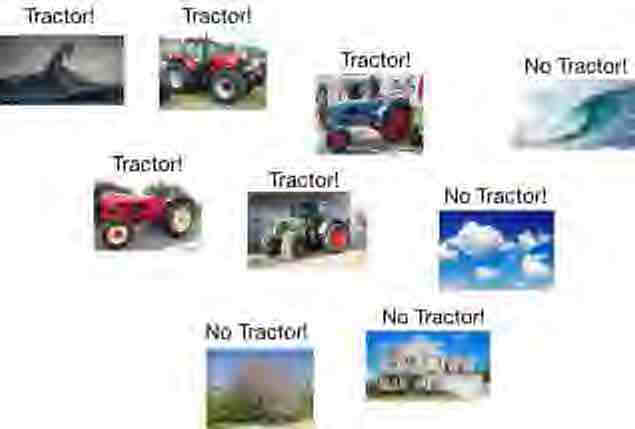
\includegraphics[width=0.7\textwidth]{LabeledDataTractorOverfitting1.jpg}  
	\caption{A (misleading) training dataset $\trainset \!=\! \{ (\vx^{(\sampleidx)},y^{(\sampleidx)}) \}_{\sampleidx=1}^{\samplesize_{\rm t}}$ 
		consisting of $\samplesize_{\rm t}=9$ images. The $\sampleidx$-th image is characterized by the feature vector $\vx^{(\sampleidx)} \in \mathbb{R}^{\featuredim}$ and labeled with $y^{(\sampleidx)}\!=\!1$ 
		(tractor) or with $y^{(\sampleidx)}\!=\!-1$ (no tractor).}
	%    \caption{Hypothesis Map}\label{fig:Hypothesis Map}
	\label{fig_misleading_data_set}
\end{figure}


\begin{figure}[htbp]
	\centering
	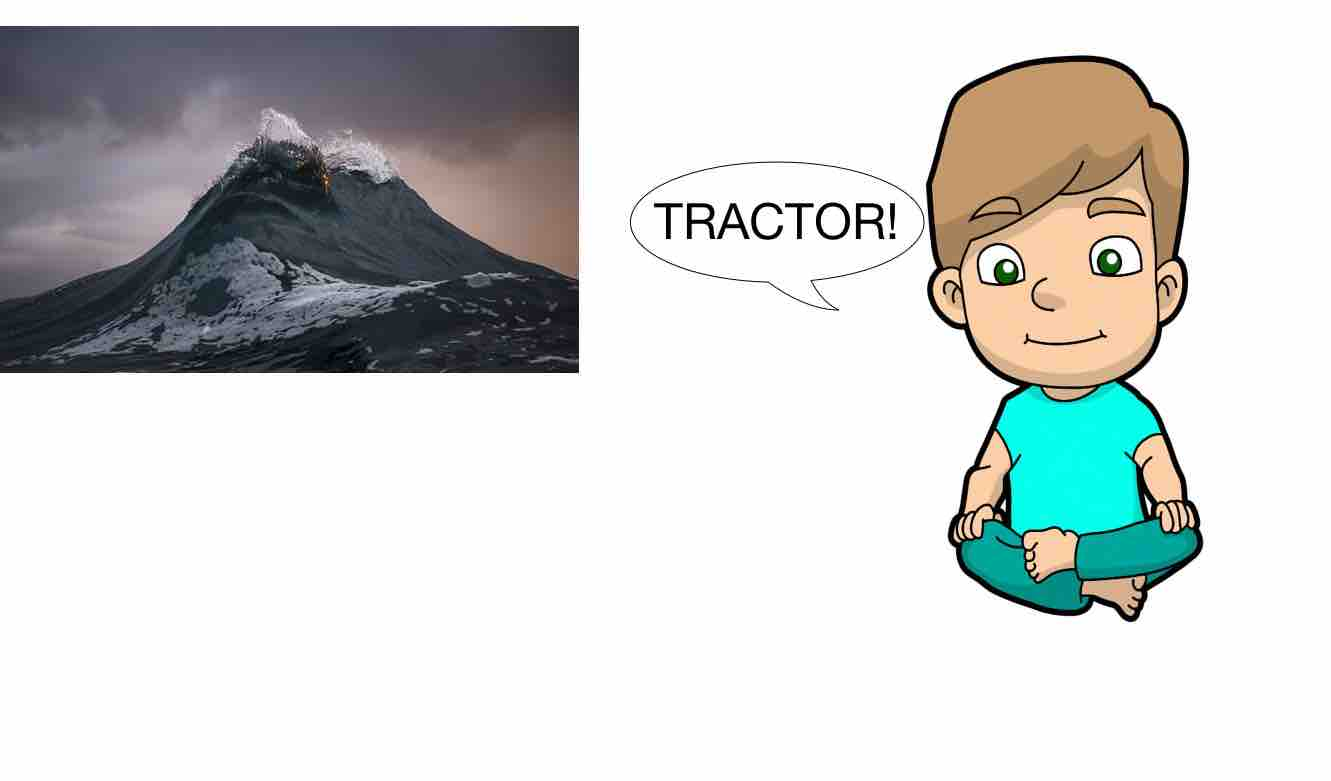
\includegraphics[width=0.7\textwidth]{OverfittingSample.jpg}   
	\caption{The child, who has been taught the concept ``tractor'' using the image collection 
		$\trainset$ in Figure \ref{fig_misleading_data_set}, might ``see'' a lot of tractors during the next beach holiday.}
	\label{equ_wave_as_tractor}   
\end{figure}


For the sake of argument, we assume that the child uses a linear predictor 
$h^{(\vw)}(\vx) = \vx^{T} \vw$, using the features $\vx$ of the image, and encodes 
the fact of showing a tractor by $y=1$ and if it is not showing a tractor by $y=-1$. 
We learn the weight vector by minimizing the squared error loss \eqref{equ_def_cost_MSE} 
on the training dataset $\dataset^{(\rm train)}$.

If we stack the feature vectors $\vx^{(\sampleidx)}$ and labels $y^{(\sampleidx)}$ into 
the feature matrix $\mX=(\vx^{(1)},\ldots,\vx^{(\samplesize_{\rm t})})^{T}$ and label 
vector $\vy=(y^{(1)},\ldots,y^{(\samplesize_{\rm t})})^{T}$, the optimal linear predictor 
is obtained for the weight vector solving \eqref{equ_zero_gradient_lin_reg} 
and the associated training error is given by \eqref{equ_emp_risk_lin_proje}, which 
we repeat here for convenience: 
\begin{equation}
\emperror(h^{(\vw_{\rm opt})} \mid \trainset) = \min_{\vw \in \mathbb{R}^{\featuredim}} \emperror(h^{(\vw)} \mid \trainset) = \|  (\mathbf{I}- \mathbf{P}) \vy \|^{2}.
\end{equation} 
Here, we used the orthogonal projection matrix $\mathbf{P}$ on the linear span 
\begin{equation} 
\nonumber
{\rm span}\{ \mX \} = \big\{  \mX \va : \va \in \mathbb{R}^{\featuredim} \big\} \subseteq \mathbb{R}^{\samplesize_{\rm t}} , 
\end{equation}
of the feature matrix 
\begin{equation} 
\label{equ_feature_matrix_overfit}
\mX = (\vx^{(1)},\ldots,\vx^{(\samplesize_{\rm t})})^{T} \in \mathbb{R}^{  \samplesize_{\rm t} \times \featuredim}. 
\end{equation} 

ML methods using linear predictors overfit as soon as the 
number $\featuredim$ of features exceeds the sample size $\samplesize$,
\begin{equation} 
\label{equ_condition_overfitting}
\featuredim  \geq \samplesize. 
\end{equation} 

A set of $\samplesize$ feature vectors $\vx^{(\sampleidx)} \in \mathbb{R}^{\featuredim}$ 
is typically linearly independent whenever \eqref{equ_condition_overfitting} is satisfied. 
If the feature vectors of the training datapoints are linearly independent, 
the span of the transposed feature matrix \eqref{equ_feature_matrix_overfit} 
coincides with $\mathbb{R}^{\samplesize}$ which implies, in turn, $\mathbf{P} = \mathbf{I}$. 

Inserting $\mathbf{P} = \mathbf{I}$ into \eqref{equ_emp_risk_lin_proje} yields 
\begin{equation}
\label{eq_zero_trianing_error}
\emperror(h^{(\vw_{\rm opt})} \mid \dataset^{(\rm train)}) = 0.
\end{equation} 
To sum up: as soon as the number  $\samplesize_{\rm t} = | \dataset_{\rm train}|$ 
of training datapoints is smaller than the number $\featuredim$ of features $\vx$, there 
is a linear predictor $h^{(\vw_{\rm opt})}$ achieving {\bf zero empirical risk} 
(see \eqref{eq_zero_trianing_error}) on the training data. The result 
\eqref{eq_zero_trianing_error} only applies if the feature vectors of 
the training datapoints are linearly independent. 

It can be shown that if the feature vectors $\vx^{(1)},\ldots,\vx^{(\samplesize)} \in \mathbb{R}^{\featuredim}$ 
are realizations of i.i.d.\ RVs with a continuous probability distribution, 
then with probability one they are linearly independent whenever \eqref{equ_condition_overfitting} holds. 

While the learnt predictor $h^{(\vw_{\rm opt})}$ is perfectly accurate on the training 
data (the training error is zero!), it will typically incur a non-zero average prediction error 
$y - h^{(\vw_{\rm opt})}(\vx)$ on new datapoints $(\vx,y)$ (which are different from the 
training data). 

Using a simple toy model for the data generation, we obtained the expression 
\eqref{equ_decomp_E_pred_toy_model} for the average prediction error. This 
average prediction error is lower bounded by the noise variance $\sigma^{2}$ 
which might be very large even when the training error is zero. Thus, when a 
method overfits, a small training error can be highly misleading regarding the 
average prediction error of a hypothesis. 

A simple, yet quite useful, strategy to detect if a predictor $\hat{h}$ overfits the training 
dataset $\dataset^{(\rm train)}$, is to compare the resulting training error 
$\emperror(\hat{h}| \dataset^{(\rm train)})$ (see \eqref{equ_def_training_error_val}) with the 
validation error $\emperror(\hat{h}| \dataset^{(\rm val)})$ (see \eqref{equ_def_training_val_val}). 
The validation error $\emperror(\hat{h}| \dataset^{(\rm val)})$ is the empirical risk of the predictor 
$\hat{h}$ on the validation dataset $\dataset^{(\rm val)}$. If overfitting occurs, the validation 
error $\emperror(\hat{h}| \dataset^{(\rm val)})$ is significantly larger than the training error 
$\emperror(\hat{h}| \dataset^{(\rm train)})$. The occurrence of overfitting for polynomial regression with 
degree $\featuredim$ (see Section \ref{sec_polynomial_regression}) chosen too large is depicted in 
Figure \ref{fig_polyn_training}. 

\begin{figure}[htbp]
	\centering
	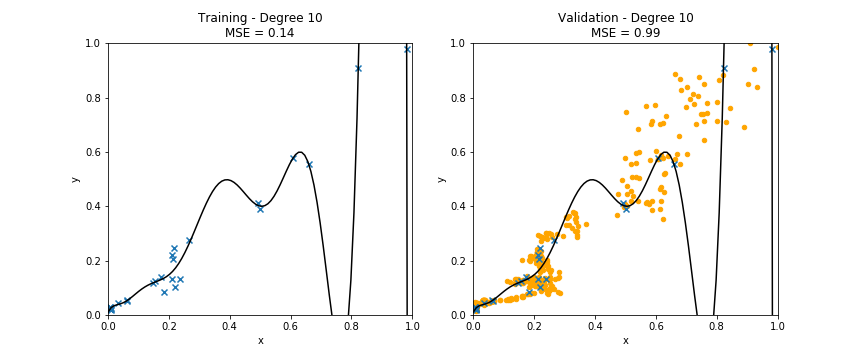
\includegraphics[width=\textwidth]{OverfittedPolyn.png}  
	\caption{The training dataset consists of the blue crosses and can be almost perfectly 
		fit by a high-degree polynomial. This high-degree polynomial gives only poor results 
		for a different (validation) dataset indicated by the orange dots.}
	\label{fig_polyn_training}
\end{figure}


\section{Validation}
\label{sec_validate_predictor}

\begin{figure}
	\begin{center}
		\begin{tikzpicture}[scale=0.9]
		
	%	\draw [thick] (5,2.5) circle (0.1cm)node[anchor=west] {\hspace*{0mm}$\vx^{(3)}$};
	%	\draw [thick] (4,2) circle (0.1cm)node[anchor=west] {\hspace*{0mm}$\vx^{(4)}$};
	%	\draw [thick] (5,1) circle (0.1cm)node[anchor=west,above] {\hspace*{0mm}$\vx^{(2)}$};
		\draw [thick] (-1,5) rectangle ++(0.1cm,0.1cm) node[anchor=west,above] {\hspace*{0mm}$\big(\vx^{(1)},y^{(1)}\big)$};
		\draw [thick] (1,3.5) rectangle ++(0.1cm,0.1cm) node[anchor=west,above] {\hspace*{0mm}$\big(\vx^{(2)},y^{(2)}\big)$};
		\draw [thick] (3,2.5) rectangle ++(0.1cm,0.1cm) node[anchor=west,above] {\hspace*{0mm}$\big(\vx^{(3)},y^{(3)}\big)$};
		 \draw [dashed] {[rounded corners] (0,7) -- (6,2)  -- (2,0) -- (-3,5) -- (0,7) };
		\node[anchor=east,above] at (2,1) {$\trainset$};
		\draw [thick] (7,4) rectangle ++(0.1cm,0.1cm) node[anchor=west,above] {\hspace*{0mm}$\big(\vx^{(4)},y^{(4)}\big)$};
		\draw [thick] (6,6) rectangle ++(0.1cm,0.1cm) node[anchor=west,above] {\hspace*{0mm}$\big(\vx^{(5)},y^{(5)}\big)$};
	    \node[anchor=east,above] at (5,5) {$\valset$};
		 \draw [dashed] {[rounded corners] (4,5) -- (5,8)  -- (7,8) -- (9,3) -- (4,5) };
	%	\draw [thick] \boundellipse{5,5}{3}{5} node[right]  {${\bm \mu^{(1)}}$};
	%	\fill (0,0) circle (2pt) ; 
	%	\node [right] at (0,5.5) {$ {\bm \Sigma}^{(1)}$} ; 
	%	\draw [thick] \boundellipse{11,1}{-2}{4} node[right]  {${\bm \mu^{(2)}}$};
	%	\fill (11,1) circle (2pt) ; 
	%	\node [right] at (11,5.5) {$ {\bm \Sigma}^{(2)}$} ; 
	%	\draw [thick] \boundellipse{-9,4}{2}{3} node[left,xshift=3mm,yshift=3mm]  {$\,\,{\bm \mu^{(3)}}$}; 
	%	\fill (-9,4) circle (2pt) ; 
	%	\node [right] at (-9,8) {$ {\bm \Sigma}^{(3)}$} ; 
		\end{tikzpicture}
	\end{center}
	\caption{We split the entire dataset $\dataset$, constituted by datapoints with features $\vx^{(\sampleidx)}$ 
		and label $y^{(\sampleidx)}$, into a {\bf training set} $\trainset$ and a {\bf validation set} 
		$\valset$. We use the training set to learn (find) the hypothesis $\hat{h}$ with minimum 
		empirical risk $\emperror(\hat{h}| \trainset)$ on the training set \eqref{equ_def_ERM_funs}. 
		We then validate $\hat{h}$ by computing its average loss $\emperror(\hat{h}| \dataset^{(\rm val)})$  
		on the validation set $\valset$. The average loss $\emperror(\hat{h}| \valset)$ obtained on the validation 
		set is the {\bf validation error}. Note that $\hat{h}$ depends on the training set $\trainset$ but is completely 
		independent of the validation set $\valset$.}
		\label{fig_split_train_val}
\end{figure}
%\end{document}

%   \caption{}
%\label{fig_split_train_val}

%\begin{figure}[htbp]
%	\begin{center}
%		\begin{tikzpicture}[auto,scale=0.8]
%
%		\draw[->] (-0.5,0) -- (6.5,0) node[right] {$x_{\rm g}$};
%		\draw[->] (0,-0.5) -- (0,6.5) node[above] {$x_{\rm r}$};
%		%\foreach \y/\ytext in { 1/1,2/2,3/3,4/4,5/5} \draw[shift={(0,\y)}] (2pt,0pt) -- (-2pt,0pt) node[left] {$\ytext/5$};  
%		%\foreach \x/\xtext in{ 1/1,2/2,3/3,4/4,5/5}\draw[shift={(\x,0)}] (0pt,2pt) -- (0pt,-2pt) node[below] {$\xtext/5$};  
%		\end{tikzpicture}
%	\end{center}
%	\caption{A scatterplot depicting some images. The $\sampleidx$-th image is 
%		represented by the feature vector $\vx^{(\sampleidx)}=(x^{(\sampleidx)}_{\rm r},x^{(\sampleidx)}_{\rm g})^{T}$ 
%		with the average redness $x_{\rm r}^{(\sampleidx)}$ and average greenness $x_{\rm g}^{(\sampleidx)}$ of the image. 
%	} 
%	\label{fig_scatterplot_clustering}
%\end{figure}

Consider an ML method using the hypothesis space $\hypospace$ that  
learns a hypothesis $\hat{h} \in \hypospace$ by ERM \eqref{equ_def_ERM_funs}. 
The hypothesis $\hat{h}$ has minimum average loss (training error) on the 
labeled dataset $\dataset$. The basic idea of validating the predictor $\hat{h}$ 
is simple: compute the empirical risk of $\hat{h}$ on a new set of datapoints $(\vx,y)$ 
which have not been already used for training. 

It is very important to validate the predictor $\hat{h}$ using labeled data 
points which do not belong to the dataset which has been used to learn 
$\hat{h}$ (e.g., via ERM \eqref{equ_def_ERM_funs}). The hypothesis 
$\hat{h}$ tends to ``look better'' on the training set than for other 
datapoints, since it is optimized precisely for the datapoints in the 
training set. 
\vspace*{2mm}
\begin{center}
\framebox[0.96\textwidth]{
 \parbox{0.9\textwidth}{
\begin{quote}
A golden rule of ML practice: use different datapoints for the learning 
(see \eqref{equ_def_ERM_funs}) and the validation of a hypothesis $\hat{h}$!
\end{quote}
}}
\end{center}
 
To validate the hypothesis learnt by a ML method we can use the following steps. 
\begin{enumerate} 
\item We randomly divide (``split'') the entire set $\dataset$ of labeled datapoints into 
two disjoint subsets $\dataset = \trainset \cup \valset$ (see Figure \ref{fig_split_train_val}). 
The first subset $\trainset$ is referred to as the {\bf training set}. The second subset $\valset$ 
is referred to as the {\bf validation set}.  
\item We learn a hypothesis $\hat{h}$ via ERM using the training data $\trainset$ (cf.\ \eqref{equ_def_ERM_funs}), 
\begin{align} 
\label{equ_def_hat_h_fitting}
\hat{h} & = \argmin_{h \in \hypospace} \emperror(h| \trainset) \nonumber \\
& = \argmin_{h \in \hypospace}  (1/\samplesize_{\rm t}) \sum_{(\vx,y) \in \trainset} \loss{(\vx,y)}{h} %( y- h(\vx))^2
\end{align} 
with corresponding {\bf training error} 
\begin{equation} 
\label{equ_def_training_error_val}
\emperror(\hat{h}|\trainset)=  (1/\samplesize_{\rm t})\sum_{(\vx,y) \in \trainset}  \loss{(\vx,y)} {\hat{h}}.  %( y- \hat{h}(\vx))^2.
\end{equation}  
\item We validate the hypothesis $\hat{h}$ obtained from \eqref{equ_def_hat_h_fitting} by computing the empirical risk 
\begin{equation} 
\label{equ_def_training_val_val}
\emperror(\hat{h}|\valset) = (1/\samplesize_{\rm v})  \sum_{(\vx,y) \in \valset} \loss{(\vx,y)} {\hat{h}}  % ( y- \hat{h}(\vx))^2, 
\end{equation}  
on the {\bf validation set} $\dataset^{(\rm val)}$. We refer to $\emperror(\hat{h}| \dataset^{(\rm val)})$ 
as the {\bf validation error} of $\hat{h}$. 
\end{enumerate} 
The choice of the split ratio (between the size of training and validation set) $|\dataset^{(\rm val)}| / |\dataset^{(\rm train)}|$ 
is often based on trial and error. It is difficult to make a precise statement on 
how to choose the split ratio which applies broadly \cite{Larsen1999}. 

The optimal choice for the size of training and validation set depends on the 
statistical properties of the datapoints. If we know the probability distribution 
from which datapoints are drawn, we can derive lower bounds on the size of 
the validation set such that the validation error \eqref{equ_def_training_val_val} 
is close to the expected loss $\expect\{ \loss{(\vx,y)} {\hat{h}} \}$ with high probability. 
 
% \begin{figure}[htbp]
%    \centering
%   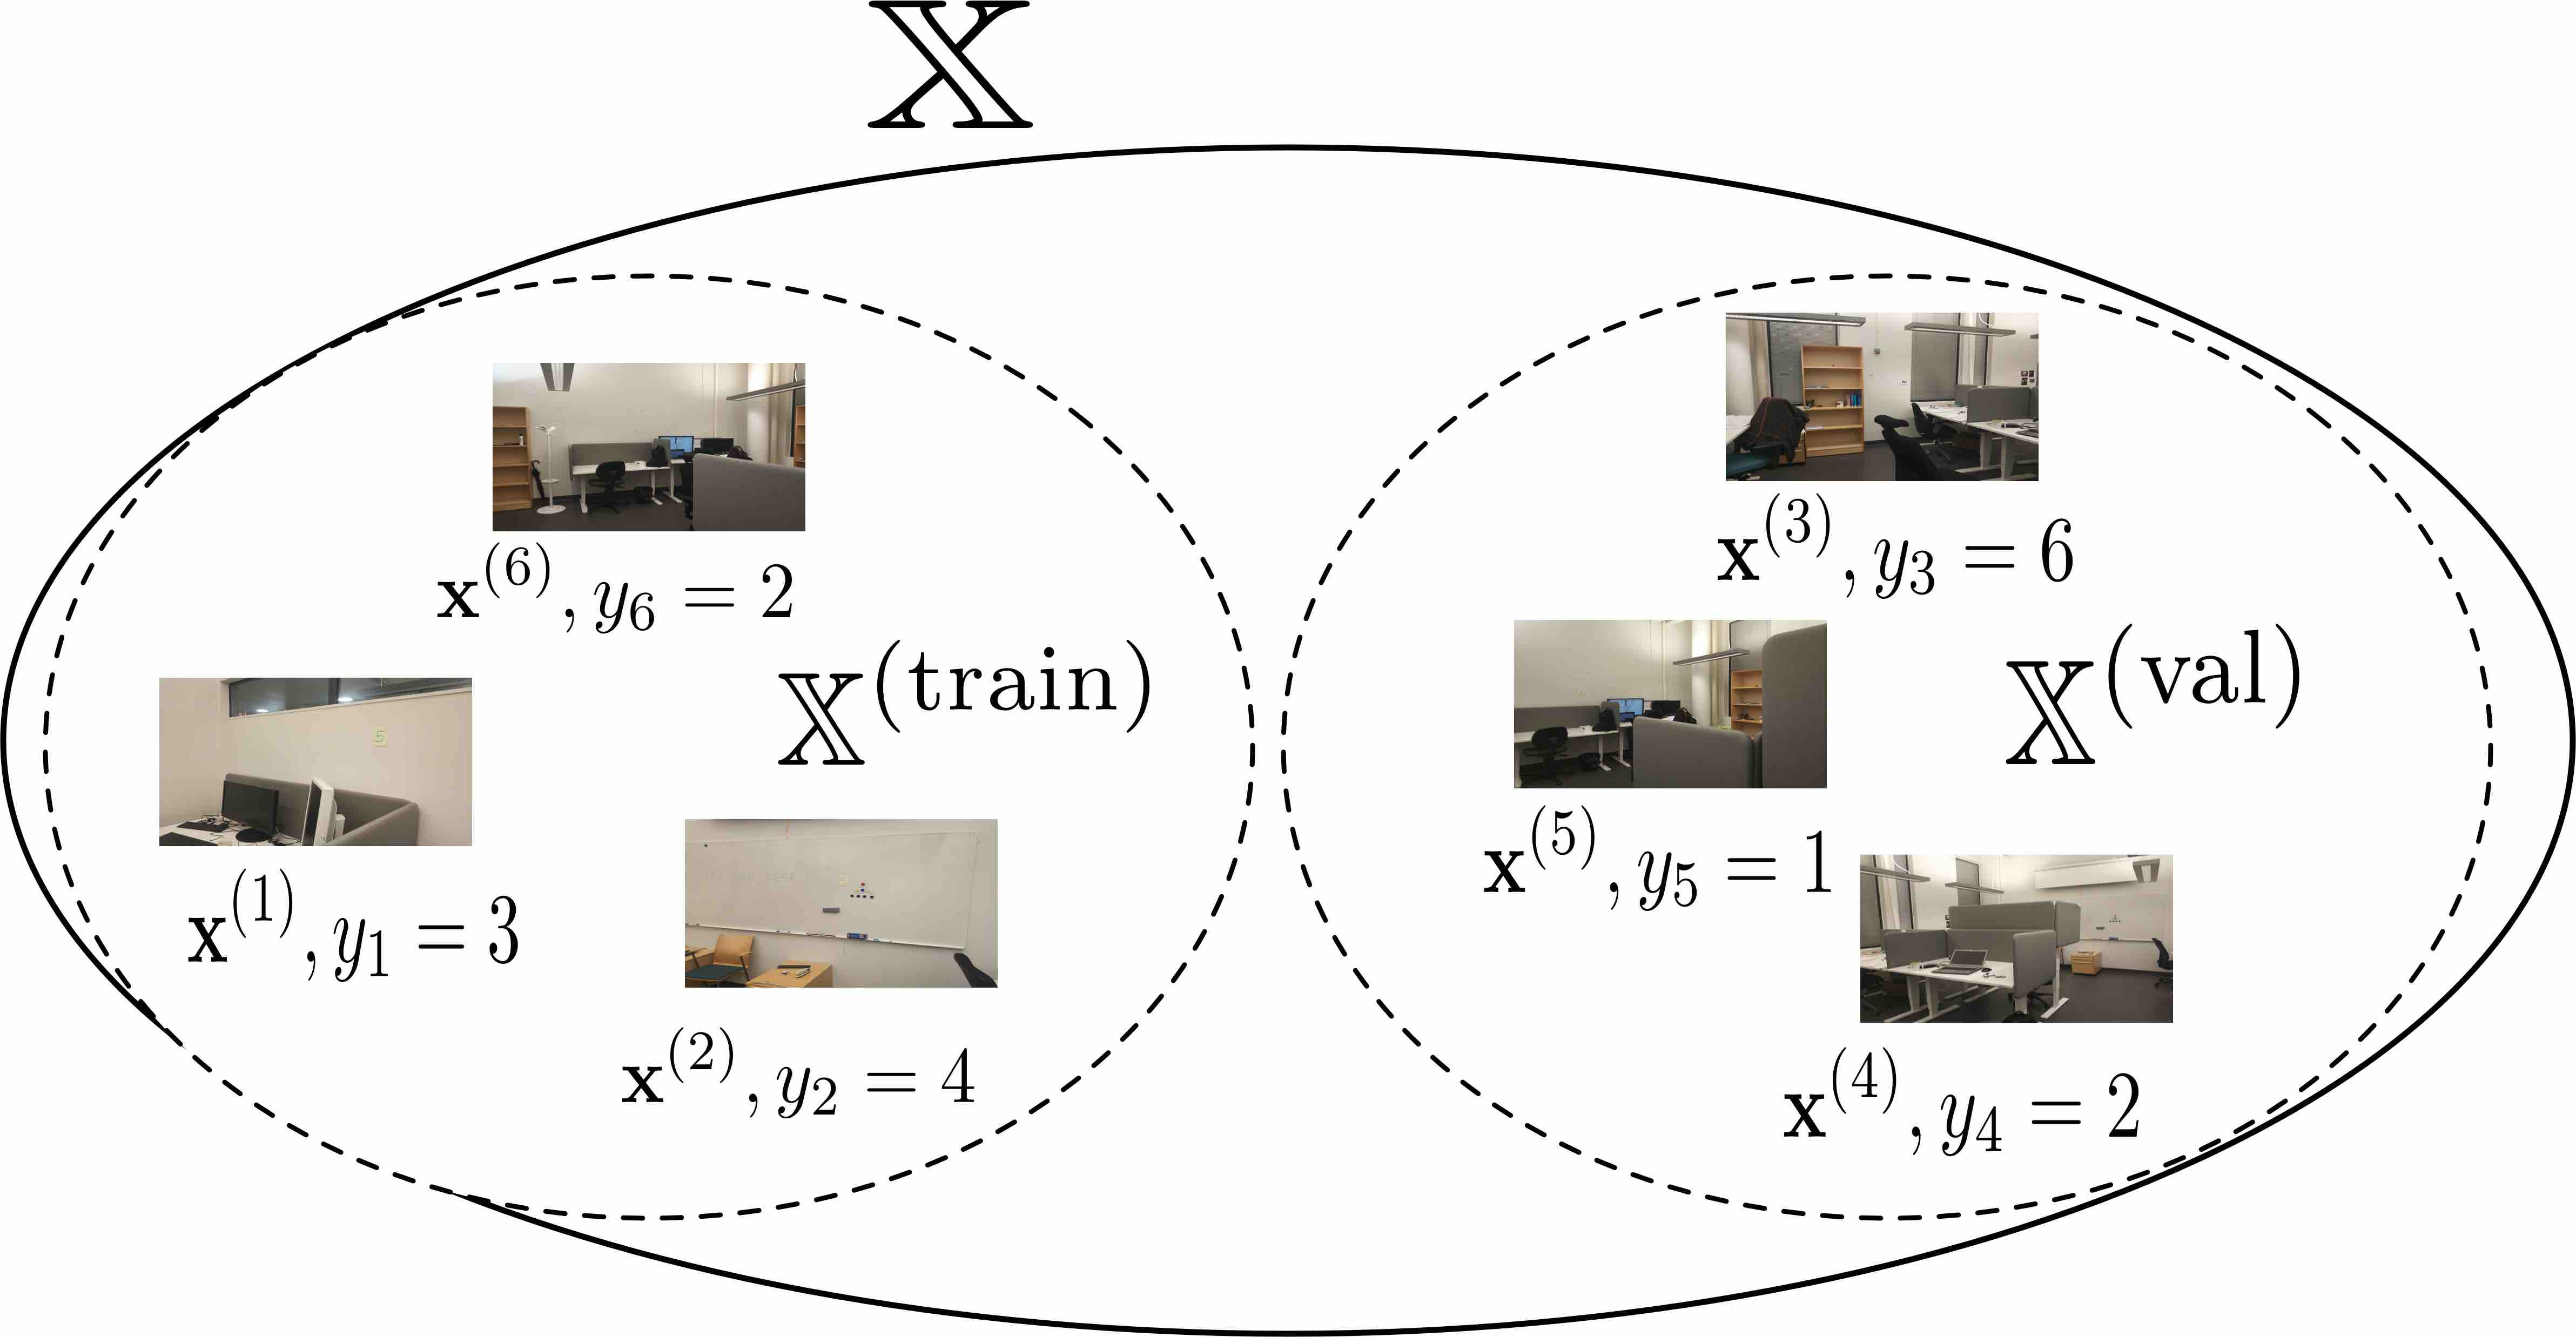
\includegraphics[width=0.7\textwidth]{TrainValSmall.jpg}  
%    \caption{We split the available dataset $\dataset$ into a 
%    	{\bf training set} $\dataset^{(\rm train)}$ and a {\bf validation set} 
%    	$\dataset^{(\rm val)}$. We use the training set in order to 
%    	learn (find) a good predictor $\hat{h}$ with minimum 
%    	empirical risk $\emperror(\hat{h}| \dataset^{(\rm train)})$ on the training set \eqref{equ_def_ERM_funs}. 
%        We then validate $\hat{h}$ by computing its empirical risk $\emperror(h| \dataset^{(\rm val)})$  
%        on the validation set $\dataset^{(\rm val)}$. The empirical risk $\emperror(h| \dataset^{(\rm val)})$ 
%        obtained on the validation set is the {\bf validation error}.}
%    \label{fig_split_train_val}
%\end{figure}

The basic idea of randomly splitting the available labeled data into training and 
validation sets underlies many validation techniques. A popular extension 
of the above approach, which is known as $k$-fold cross-validation, is based 
on repeating the splitting into training and validation sets $k$ times. During 
each repetition, this method uses different subsets for training and validation. 
We refer to \cite[Sec. 7.10]{hastie01statisticallearning} for a detailed discussion of $k$-fold 
cross-validation. 

{\bf Imbalanced Data.} 
The simple validation approach discussed above requires the validation set to be 
a good representative for the overall statistical properties of the data. This might 
not be the case in applications with discrete valued labels and some of the label 
values being very rare. 

Consider datapoints characterized by a feature vector $\vx$ and binary label $y \in \{-1,1\}$. 
Assume we aim at learning a hypothesis $h(\vx) = \vw^{T} \vx$ to classify datapoints 
via $\hat{y}=1$ if $h(\vx) \geq 0$ while $\hat{y}=-1$ otherwise. The learning is based 
on a dataset $\dataset$ which contains only one single (!) datapoint with $y=-1$. If 
we then split the dataset into training and validation set, it is with high probability that 
the validation set does not include any datapoint with $y=-1$. This cannot happen 
when using $k$-fold CV since the single data point must be one of the validation folds. 
However, even when using $k$-fold CV for such an imbalanced dataset is problematic since 
we evaluate the performance of a hypothesis $h(\vx)$ using only one single 
datapoint with $y=-1$. The validation error will then be dominated by the performance 
of $h(\vx)$ only on datapoints with $y=1$. 


\section{Model Selection}
\label{sec_modsel}

We will now discuss how to use the validation principle of 
Section \ref{sec_validate_predictor} to perform model selection. 
As discussed in Chapter \ref{ch_Elements_ML}, the choice of 
the hypothesis space from which we select a predictor map 
(e.g., via solving the ERM \eqref{equ_def_ERM_funs}) is a design choice. 
However, it is often not obvious what a good first choice 
for the hypothesis space is. We might try out different 
choices $\hypospace_{1},\hypospace_{2},\ldots,\hypospace_{M}$ 
for the hypothesis space. 

Consider datapoints with a non-linear relation between its 
feature $x$ and label $y$. We might then use polynomial 
regression (see Section \ref{sec_polynomial_regression}) 
using the hypothesis space $\hypospace_{\rm poly}^{(\featuredim)}$ 
with some maximum degree $\featuredim$. 

Different choices for the maximum degree $\featuredim$ yield 
a different hypothesis space: $\hypospace_{1} = \mathcal{H}_{\rm poly}^{(0)},\hypospace_{2} = \mathcal{H}_{\rm poly}^{(1)},\ldots,\hypospace_{M} = \hypospace_{\rm poly}^{(M-1)}$. 
We might also mix polynomial maps using maps obtained from  
Gaussian basis functions (see Section \ref{sec_linbasreg}), 
with different choices for the variance $\sigma$ and shifts $\mu$ 
of the Gaussian basis function \eqref{equ_basis_Gaussian}, 
e.g., $\hypospace_{1} = \mathcal{H}^{(2)}_{\rm Gauss}$ with $\sigma=1$ and $\mu_{1}=1$ and $\mu_{2}=2$, 
$\hypospace_{2} = \hypospace^{(2)}_{\rm Gauss}$ with $\sigma = 1/10$, $\mu_{1}=10$, $\mu_{2}= 20$.

A principled approach for choosing a hypothesis space out of a  
list of candidate spaces $\hypospace_{1},\hypospace_{2},\ldots,\hypospace_{M}$ 
is as follows: 
\begin{itemize} 
\item randomly divide (split) the entire dataset $\dataset$ of labeled snapshots into two disjoint subsets 
$\trainset$ (the ``training set'') and $\valset$ (the ''validation set''): 
$\dataset = \trainset \cup \valset$ (see Figure \ref{fig_split_train_val}). 
\item for each hypothesis space $\hypospace_{l}$ learn predictor $\hat{h}_{l} \in \hypospace_{l}$ via ERM \eqref{equ_def_ERM_funs} using training data $\trainset$:
\begin{align} 
\label{equ_def_hat_h_fitting_sel}
\hat{h}_{l} & = \argmin_{h \in \hypospace_{l}} \emperror(h| \trainset) \nonumber \\
& = \argmin_{h \in \hypospace_{l}}  (1/\samplesize_{\rm t}) \sum_{\sampleidx=1}^{\samplesize_{\rm t}} \loss{(\vx^{(\sampleidx)},y^{(\sampleidx)})}{h} %( y- h(\vx))^2
\end{align} 
\item compute the validation error of $\hat{h}_{l}$ 
\begin{equation} 
\label{equ_def_training_val_val_modsel}
\emperror(\hat{h}_{l}|\valset) = (1/\samplesize_{\rm v}) \sum_{\sampleidx=1}^{\samplesize_{\rm v}} \loss{(\vx^{(\sampleidx)},y^{(\sampleidx)})} {\hat{h}_{l}}  % ( y- \hat{h}(\vx))^2, 
\end{equation}  
obtained when applying the predictor $\hat{h}_{l}$ to the {\bf validation dataset} $\valset$. 
\item pick the hypothesis space $\hypospace_{l}$ resulting in the smallest validation error $\emperror(\hat{h}_{l}|\valset)$
\end{itemize} 



\section{A Probabilistic Analysis of Generalization} 
\label{sec_gen_linreg}
\emph{More Data Beats Clever Algorithms ?; More Data Beats Clever Feature Selection?}

A key challenge in ML is the ensure that a hypothesis that predicts well 
the labels of training datapoints will also predict well the labels of datapoints 
outside the training set. We say that a ML method generalizes if a small 
loss on the training set implies small loss on other datapoints as well. 

To study generalization within a linear regression problem 
(see Section \ref{sec_lin_regression}), we will use a {\bf probabilistic model} 
for the data. We interpret datapoints as i.i.d. realizations of RVs that have 
the same distribution as a random datapoint $\vz=(\vx,y)$. The random 
feature vector $\vx$ is assumed to have zero mean and covariance 
being the identity matrix, i.e., $\vx \sim \mathcal{N}(\mathbf{0}, \mathbf{I})$. 
The label $y$ of a random datapoint is related to its features $\vx$ via a 
{\bf linear Gaussian model} 
\begin{equation} 
\label{equ_linear_obs_model}
y = \bar{\vw}^{T}  \vx + \varepsilon \mbox{, with noise } \varepsilon \sim \mathcal{N}(0,\sigma^{2}).
\end{equation} 
We assume the noise variance $\sigma^{2}$ fixed and known. This is a simplifying assumption as in 
practice, we would need to estimate the noise variance from data \cite{Cohen2002}. Note that, within 
our probabilistic model, the error component $\varepsilon$ in \eqref{equ_linear_obs_model} is intrinsic 
to the data and cannot be overcome by any ML method. We highlight that the probabilistic model for 
the observed data points is just a modelling assumption. This assumption allows us to study some 
fundamental behaviour of ML methods. There are principled statistical that allow to determine if 
given datapoints can be accurately modelled using \eqref{equ_linear_obs_model} \cite{}. 

We predict the label $y$ from the features $\vx$ using a linear hypothesis $h(\vx)$ 
that depends only on the first $r$ features $x_{1},\ldots,x_{r}$. Thus, we use the 
hypothesis space 
\vspace*{-2mm}
\begin{equation}
\label{equ_generalization_hypospace_r}
\hypospace^{(r)} = \{ h^{(\vw)}(\vx)= (\vw^{T},\mathbf{0}) \vx \mbox{ with } \mathbf{w} \in \mathbb{R}^{r} \}.   
\vspace*{-1mm}
\end{equation}
The design parameter $r$ determines the size of the hypothesis space 
$\hypospace^{(r)}$ and, in turn, the computational complexity of learning 
the optimal hypothesis in $\hypospace^{(r)}$. 

For $r < \featuredim$, the hypothesis space $\hypospace^{(r)}$ 
is a proper subset of the space of linear predictors \eqref{equ_def_hypo_linear_pred} 
used within linear regression (see Section \ref{sec_lin_regression}). Note that 
each element $h^{(\vw)} \in \hypospace^{(r)}$ corresponds to a particular 
choice of the weight vector $\vw \in \mathbb{R}^{r}$. 

The quality of a particular predictor $h^{(\vw)} \in \hypospace^{(r)}$ is measured 
via the mean squared error $\emperror (h^{(\vw)} \mid \trainset)$ incurred over a 
labeled training set $\trainset= \{ \vx^{(\sampleidx)}, y^{(\sampleidx)} \}_{\sampleidx=1}^{\samplesize_{\rm t}}$. 
Within our toy model (see \eqref{equ_linear_obs_model}, \eqref{equ_toy_model_iid} 
and \eqref{equ_labels_training_data}), the training datapoints $(\vx^{(\sampleidx)},y^{(\sampleidx)})$ 
are i.i.d.\ copies of the datapoint $\vz = (\vx,y)$. 

The datapoints in the training dataset and any other datapoints outside the 
training set are statistically independent. However, the training datapoints 
$(\vx^{(\sampleidx)},y^{(\sampleidx)})$ and any other datapoint $(\vx,y)$ are 
drawn from  the same probability distribution, which is a multivariate normal distribution, 
\begin{equation} 
\label{equ_toy_model_iid}
\vx, \vx^{(\sampleidx)} \mbox{ i.i.d. with } \vx, \vx^{(\sampleidx)} \sim \mathcal{N}(\mathbf{0}, \mathbf{I}) 
\end{equation} 
and the labels $y^{(\sampleidx)},y$ are obtained as 
\begin{equation} 
\label{equ_labels_training_data}
y^{(\sampleidx)} = \bar{\vw}^{T}  \vx^{(\sampleidx)} + \varepsilon^{(\sampleidx)}\mbox{, and } y = \bar{\vw}^{T}  \vx + \varepsilon
\end{equation}  
with i.i.d.\ noise $\varepsilon, \varepsilon^{(\sampleidx)} \sim \mathcal{N}(0,\sigma^{2})$. 

As discussed in Chapter \ref{ch_Optimization}, the training error $\emperror (h^{(\vw)} \mid \trainset)$ 
is minimized by the predictor $h^{(\hat{\vw})}(\vx) =  \hat{\vw}^{T} \mathbf{I}_{r \times \featuredim} \vx$, 
with weight vector 
\begin{equation}
\label{equ_optimal_weight_closed_form}
\widehat{\vw} =  (\mX^{T}_{r} \mX_{r})^{-1} \mX_{r}^{T} \vy
\end{equation} 
with feature matrix $\mX_{r}$ and label vector $\vy$ defined as 
\begin{align}
\label{equ_def_feature_matrix_r}
\mX_{r}& \!=\!(\vx^{(1)},\ldots,\vx^{(\samplesize_{\rm t})})^{T} \mathbf{I}_{\featuredim \times r}\!\in\!\mathbb{R}^{\samplesize_{\rm t} \times r} \mbox{, and }  \nonumber \\
\vy& \!=\!\big(y^{(1)},\ldots,y^{(\samplesize_{\rm t})}\big)^{T}\!\in\!\mathbb{R}^{\samplesize_{\rm t}}.
\end{align} 

It will be convenient to tolerate a slight abuse of notation and denote both, 
the length-$r$ vector \eqref{equ_optimal_weight_closed_form} as well as the zero 
padded length-$\featuredim$ vector $(\widehat{\vw}^{T},\mathbf{0})^{T}$, by $\widehat{\vw}$. 
This allows us to write % the predictor $h^{(\hat{\vw})}(\vx)$ as 
\begin{equation} 
h^{(\widehat{\vw})}(\vx) = \widehat{\vw}^{T} \vx. 
\end{equation}

We highlight that the formula \eqref{equ_optimal_weight_closed_form} 
for the optimal weight vector $\widehat{\vw}$ is only valid if the matrix 
$\mX^{T}_{r} \mX_{r}$ is invertible. However, it can be shown that within 
our toy model (see \eqref{equ_toy_model_iid}), this is true with probability 
one whenever $\samplesize_{\rm t} \geq r$. In what follows, we will consider 
the case of having more training samples than the dimension of the 
hypothesis space, i.e., $\samplesize_{\rm t} > r$ such that the formula 
\eqref{equ_optimal_weight_closed_form} is valid (with probability one). 
The case $\samplesize_{\rm t} \leq r$ will be studied in Chapter \ref{ch_overfitting_regularization}.

The optimal weight vector $\widehat{\vw}$ (see \eqref{equ_optimal_weight_closed_form}) 
depends on the training data $\trainset$ via the feature matrix $\mX_{r}$ 
and label vector $\vy$ (see \eqref{equ_def_feature_matrix_r}). Therefore, 
since we model the training data as random, the weight vector $\widehat{\vw}$ 
\eqref{equ_optimal_weight_closed_form} is a random quantity. For each different 
realization of the training dataset, we obtain a different realization of the 
optimal weight $\widehat{\vw}$. 

The probabilistic model \eqref{equ_linear_obs_model} relates the features 
$\vx$ of a datapoint to its label $y$ via some (unknown) true weight vector $\bar{\vw}$. 
Intuitively, the best linear hypothesis would be $h(\vx) =\widehat{\vw}^{T} \vx$ with 
weight vector $\widehat{\vw} = \bar{\vw}$. However, in general this will not be 
achievable since we have to compute $\widehat{\vw}$ based on the features 
$\vx^{(\sampleidx)}$ and noisy labels $y^{(\sampleidx)}$ of the data 
points in the training dataset $\dataset$. 

In general, learning the weights of a linear hypothesis by ERM \eqref{equ_def_cost_MSE} 
results in a non-zero {\bf estimation error}
\begin{equation}
\label{equ_def_est_error}
\Delta \vw \defeq \widehat{\vw} - \bar{\vw}. 
\end{equation} 
The estimation error \eqref{equ_def_est_error} is a random quantity (realization of a random variable) 
since the learnt weight vector $\widehat{\vw}$ (see \eqref{equ_optimal_weight_closed_form}) 
is a random quantity itself.

{\bf Bias and Variance.} 
As we will see below, the prediction quality achieved by $h^{(\widehat{\vw})}$ 
depends crucially on the {\bf mean squared estimation error (MSE)}
\begin{equation}
\label{equ_def_est_err}
\mathcal{E}_{\rm est} \defeq \expect \{  \| \Delta \vw \|^{2}_{2} \} =  \expect \big\{ \big \| \widehat{\vw} - \bar{\vw} \big\|^{2}_{2} \big \}. 
\end{equation}
We can decompose the MSE $\mathcal{E}_{\rm est}$ into two components. 
The first component is the {\bf bias} which characterizes the properties of 
the learn hypothesis on average (over all different realizations of training sets). 
The second component is the {\bf variance} which quantifies the amount of 
random fluctuations of the hypothesis obtained from ERM applied to 
different realizations of the training set. Both components depend on the model 
complexity parameter $r$. 
%depends on the 
%distribution of the observed feature vectors $\vx^{(\sampleidx)}$ 
%and labels $y^{(\sampleidx)}$. 

It is not too difficult to show that 
\vspace*{-1mm}
\begin{align}
\label{equ_bias_var_decomp}
\mathcal{E}_{\rm est} & = \underbrace{ \| \bar{\vw} - \expect \{ \widehat{\vw} \} \|^{2}_{2} }_{\mbox{``bias''} B^2}+ \underbrace{\expect \| \widehat{\vw} - \expect \{ \widehat{\vw} \} \|^{2}_{2}}_{\mbox{``variance''} V} 
\end{align} 

The bias term in \eqref{equ_bias_var_decomp}, which can be computed as 
\vspace*{-3mm}
\begin{equation}
\label{equ_def_bias_term}
B^{2} = \| \bar{\vw} - \expect \{ \widehat{\vw} \} \|^{2}_{2} = \sum_{l=r+1}^{\featuredim} \bar{w}_{l}^2, 
\end{equation} 
measures the distance between the ``true hypothesis'' $h^{(\bar{\vw})}(\vx)=\bar{\vw}^{T} \vx$ 
and the hypothesis space $\hypospace^{(r)}$ (see \eqref{equ_generalization_hypospace_r}) of 
the linear regression problem. 

The bias \eqref{equ_def_bias_term} is zero if $\bar{w}_{l}=0$ for any index 
$l=r+1,\ldots,\featuredim$, or equivalently if $h^{(\bar{\vw})} \in \hypospace^{(r)}$. 
We can ensure that for every possible true weight vector $\bar{\vw}$ in \eqref{equ_linear_obs_model} 
only if we use the hypothesis space $\hypospace^{(r)}$ with $r=\featuredim$. 

When using the model $\hypospace^{(r)}$ with $r < \featuredim$, we cannot guarantee 
a zero bias term since we have no access to the true underlying weight vector $\bar{\vw}$ 
in \eqref{equ_linear_obs_model}. In general, the bias term decreases with an 
increasing model size $r$ (see Figure \ref{fig_bias_variance}). We 
highlight that the bias term does not depend on the variance 
$\sigma^{2}$ of the noise $\varepsilon$ in our toy model \eqref{equ_linear_obs_model}. 

Let us now consider the variance term in \eqref{equ_bias_var_decomp}. 
Using the properties of our toy model (see \eqref{equ_linear_obs_model}, 
\eqref{equ_toy_model_iid} and \eqref{equ_labels_training_data})
\begin{equation}
\label{equ_variance_term_toy_model}
V = \expect \{ \| \widehat{\vw} - \expect\{ \widehat{\vw} \} \|^{2}_{2} \} = \sigma^{2} \mbox{tr} \big\{ \expect\{(\mX_{r}^{T} \mX_{r})^{-1} \} \big\}.
\end{equation} 
By \eqref{equ_toy_model_iid}, the matrix $(\mX_{r}^{T} \mX_{r})^{-1}$ is 
random and distributed according to an {\bf inverse Wishart distribution} \cite{Mardia1979}. 
For $\samplesize_{\rm t} > r +1$, its expectation is given as 
\begin{equation} 
\label{equ_expr_expect_inv-wishart}
\expect\{(\mX_{r}^{T} \mX_{r})^{-1} \} = 1/(\samplesize_{\rm t}-r-1) \mathbf{I}_{r \times r}.
\end{equation} 
By inserting \eqref{equ_expr_expect_inv-wishart} and $\mbox{tr} \{ \mathbf{I}_{r \times r} \} = r$ into \eqref{equ_variance_term_toy_model}, 
\begin{equation} 
\label{equ_formulae_variance_toy_model}
V= \expect \{ \| \widehat{\vw} - \expect\{ \widehat{\vw} \} \|^{2}_{2} \} = \sigma^{2} r/(\samplesize_{\rm t}-r-1). 
\end{equation} 
As indicated by \eqref{equ_formulae_variance_toy_model}, the 
variance term increases with increasing model complexity $r$ 
(see Figure \ref{fig_bias_variance}). This behaviour is in stark 
contrast to the bias term which decreases with increasing $r$. 
The opposite dependency of bias and variance on the model 
complexity is known as the {\bf bias-variance trade-off}. Thus, 
the choice of model complexity $r$ (see \eqref{equ_generalization_hypospace_r}) 
has to balance between a small variance and a small bias. 

\begin{figure}
\begin{center}
    \begin{tikzpicture}
       \draw [thick, <->] (1,3.5) -- (1,0) -- (10.2,0);<
       \draw[red, ultra thick, domain=1:10] plot (\x,  {3*\x^-1});
                 \draw[blue, ultra thick, domain=1:10] plot (\x,  {3*\x/10});
                   \draw[ultra thick, domain=1:10,dashed] plot (\x,  {3*\x^(-1)+3*\x/10});
           \node [right, color=red] at (10.2,0.3) {bias};
                 \node [right,color=blue] at (5.2,1.4) {variance};
               \node [below] at (5,0) {model complexity $r$};
                 \node [above] at (5,2.2) {$\mathcal{E}_{\rm est}$};
     \end{tikzpicture}
\end{center}
\caption{The estimation error $\mathcal{E}_{\rm est}$ incurred by linear 
	regression can be decomposed into a bias term $B^{2}$ and a variance 
	term $V$ (see \eqref{equ_bias_var_decomp}). These two components 
	depend on the model complexity $r$ in an opposite manner resulting in 
	a bias-variance trade-off.}
\label{fig_bias_variance}
\end{figure}


{\bf Generalization.}
Consider the linear hypothesis $h(\vx) = \hat{\vw}^{T} \vx$ with the weight 
vector \eqref{equ_optimal_weight_closed_form} which results in a minimum 
training error. We would like this predictor to generalize well to datapoints 
which are different from the training set. This generalization capability can 
be quantified by the expected loss or risk %\eqref{}. 
%In most ML applications, we are primarily interested in how well a 
%predictor $h^{(\hat{\vw})}$, which has been learnt from some 
%training data $\dataset$ (see \eqref{equ_def_ERM_funs}), predicts 
%the label $y$ of a new datapoint (which is not contained in the training data $\dataset$) 
%with features $\vx$. The prediction (approximation guess or estimate) 
%$\hat{y}$ of the label $y$ is obtained using the learnt 
%predictor $h^{(\hat{\vw})}$ via  
%\begin{equation}
%\label{equ_def_pred_simple_toy_model}
%\hat{y} = \widehat{\vw}^{T} \vx. 
%\end{equation} 
%
%The prediction $\hat{y}$ is a random variable since (i) the feature vector 
%$\vx$ is modelled as a random vector (see \eqref{equ_toy_model_iid}) 
%and (ii) the optimal weight vector $\widehat{\vw}$ (see \eqref{equ_optimal_weight_closed_form}) 
%is random. In general, we cannot hope for a perfect prediction 
%but have to face a non-zero prediction error 
%\begin{align}
%\label{equ_def_pred_error}
%e_{\rm pred} & \defeq \hat{y} - y \nonumber \\ 
%& \stackrel{\eqref{equ_def_pred_simple_toy_model}}{=}\widehat{\vw}^{T} \vx - y \nonumber \\ 
%& \stackrel{\eqref{equ_linear_obs_model}}{=} \widehat{\vw}^{T} \vx - (\vw_{\rm true}^{T}  \vx + \varepsilon) \nonumber \\ 
%& = \Delta \vw^{T}  \vx - \varepsilon.
%\end{align} 
%%Within our toy model (see \eqref{equ_linear_obs_model}, \eqref{equ_toy_model_iid} 
%%and \eqref{equ_labels_training_data}), 
%The prediction error $e_{\rm pred}$ is a random variable since (i) the 
%label $y$ is modelled as a random variable (see \eqref{equ_linear_obs_model}) 
%and (ii) the prediction $\hat{y}$ is random. 
%
%Since, within our toy model \eqref{equ_labels_training_data}, $\varepsilon$ is zero-mean and independent of 
%$\vx$ and $\widehat{\vw} - \vw_{\rm true}$, we obtain the {\bf average predictor error} as 
\begin{align} 
\label{equ_decomp_E_pred_toy_model}
\mathcal{E}_{\rm pred} & = \expect \big\{ \big( y - \hat{y} \big)^2 \big\} \nonumber \\
& \stackrel{\eqref{equ_linear_obs_model}}{=} \expect \{ \Delta \vw^{T} \vx \vx^{T} \Delta \vw \} + \sigma^{2}   \nonumber \\
& \stackrel{(a)}{=} \expect \{ \expect \{ \Delta \vw^{T} \vx \vx^{T} \Delta \vw \mid \dataset \} \} + \sigma^{2}  \nonumber \\
& \stackrel{(b)}{=} \expect \{ \Delta \vw^{T} \Delta \vw \}  + \sigma^{2}  \nonumber \\
& \stackrel{\eqref{equ_def_est_error},\eqref{equ_def_est_err}}{=} \mathcal{E}_{\rm est} + \sigma^{2} \nonumber \\
& \stackrel{\eqref{equ_bias_var_decomp}}{=} B^{2} + V + \sigma^{2}. 
\end{align} 
Step (a) uses the law of total expectation \cite{BillingsleyProbMeasure} and 
step (b) uses that, conditioned on the dataset $\dataset$, the feature vector 
$\vx$ of a new datapoint is a random vector with zero mean and a 
covariance matrix $\expect \{ \vx \vx^{T}\}=\mathbf{I}$ (see \eqref{equ_toy_model_iid}). 

According to \eqref{equ_decomp_E_pred_toy_model}, the average (expected) 
prediction error $\mathcal{E}_{\rm pred}$ is the sum of three components: (i) 
the bias $B^{2}$, (ii) the variance $V$ and (iii) the noise variance $\sigma^{2}$. 
Figure \ref{fig_bias_variance} illustrates the typical dependency of the bias and 
variance on the model, which is parametrized by $r$. 

The bias and variance, whose sum is the estimation error $\mathcal{E}_{\rm est}$, 
can be influenced by varying the model complexity $r$ which is a design parameter. 
The noise variance $\sigma^{2}$ is the intrinsic accuracy limit of our toy model \eqref{equ_linear_obs_model} 
and is not under the control of the ML engineer. It is impossible for 
any ML method - no matter how advanced it is - to achieve, 
on average, a prediction error smaller than the noise variance $\sigma^{2}$. 

We finally highlight that our analysis of bias \eqref{equ_def_bias_term}, 
variance \eqref{equ_formulae_variance_toy_model} and the average prediction 
error \eqref{equ_decomp_E_pred_toy_model} only applies if the observed 
datapoints are well modelled as realizations of random vectors according 
to \eqref{equ_linear_obs_model}, \eqref{equ_toy_model_iid} and \eqref{equ_labels_training_data}. 
The usefulness of this model for the data arising in a particular application 
has to be verified in practice by some validation techniques \cite{Young93,Vasicek76}. 

An alternative approach for analyzing bias, variance and average 
prediction error of linear regression is to use simulations. Here, we 
generate a number of i.i.d.\ copies of the observed datapoints by 
some random number generator \cite{Andrieu2001}. Using these 
i.i.d.\ copies, we can replace exact computations (expectations) 
by empirical approximations (sample averages).  

\section{The Bootstrap} 

Consider learning a hypothesis $\hat{h} \in \hypospace$ by minimizing the 
average loss incurred on a dataset $\dataset=\{ \big(\vx^{(1)},y^{(1)}\big),\ldots,\big(\vx^{(\samplesize)},y^{(\samplesize)}\big)\}$. 
The datapoints $\big(\vx^{(\sampleidx))},y^{(\sampleidx)}\big)$ are modelled 
as realizations of i.i.d.\ random variables. Let use denote the (common) probability 
distribution of these random variables by $p(\vx,y)$. 

If we interpret the datapoints $\big(\vx^{(\sampleidx))},y^{(\sampleidx)}\big)$ as realizations of 
random variables, also the learnt hypothesis $\hat{h}$ is a realization  
of a random variable. Indeed, the hypothesis $\hat{h}$ is obtained by 
solving an optimization problem \eqref{equ_def_ERM_funs} that involves 
realizations of random variables. The bootstrap is a method for estimating 
(parameters of) the probability distribution $p(\hat{h})$ \cite{hastie01statisticallearning}.  

Section \ref{sec_gen_linreg} used a probabilistic model for 
datapoints to derive analytically (some parameters of) the probability 
distribution $p(\hat{h})$. While the analysis in Section \ref{sec_gen_linreg} 
only applies to the specific probabilistic model \eqref{equ_toy_model_iid}, \eqref{equ_labels_training_data}, 
the bootstrap can be used for datapoints drawn from an arbitrary 
probability distribution. 

The core idea behind the bootstrap is to use the empirical distribution 
or histogram $\hat{p}(\vz)$ of the available datapoints $\dataset$ to 
generate $B$ new datasets $\dataset^{(1)},\ldots$. Each dataset is 
constructed such that is has the same size as the original dataset $\dataset$. 
For each dataset $\dataset^{(b)}$, we solve a separate ERM \eqref{equ_def_ERM_funs} 
to obtain the hypothesis $\hat{h}^{(b)}$. The hypothesis $\hat{h}^{(b)}$ is a realization 
of a random variable whose distribution is determined by the empirical distribution 
$\hat{p}(\vz)$ as well as the hypothesis space and the loss function 
used in the ERM \eqref{equ_def_ERM_funs}. 




\section{Diagnosing ML} 
\label{equ_diagnosis_ML}
\emph{compare training, validation and benchmark error. benchmark can 
be Bayes risk when using probabilistic model (such as i.i.d.), or human 
performance or risk of some other ML methods ("experts" in regret framework)  }

Consider a ML method which learns a hypothesis $\hat{h}$ using ERM 
\eqref{equ_def_ERM_funs} on a training set $\trainset$ resulting in the 
training error 
$$\emperror(\hat{h}| \trainset) =  (1/|\trainset|) \sum_{(\vx,y) \in \trainset} \loss{(\vx,y)}{\hat{h}}.$$ 
We then validate the hypothesis by computing the validation error  
$$\emperror(\hat{h}| \dataset^{(\rm val)}) = (1/|\valset|) \sum_{(\vx,y) \in \valset} \loss{(\vx,y)}{\hat{h}}.$$ 
By comparing the two numbers $\emperror(\hat{h}| \trainset)$ and $\emperror(\hat{h}| \dataset^{(\rm val)})$ 
we diagnose the ML method. This diagnosis might provide insight into how 
the ML method could be improved. 

In some applications we might know a benchmark $\mathcal{E}_{0}$ 
for the average loss that is considered acceptable. Such a benchmark 
can be obtained using a probabilistic model for the datapoints. Given such a probabilistic 
model we can compute the minimum achievable expected loss or risk \eqref{equ_def_risk}. 
This minimum risk can often be read from the posterior distribution $p(y|\vx)$ of 
the label $y$, given the features $\vx$ of a datapoint. 

Another option to obtain such a benchmark is by considering other ML methods 
(``experts'') which are computationally more expensive. Finally, such a benchmark 
might simply be prescribed by the specification of the overall product which uses 
the ML method. 

We can diagnose a ML method by comparing the training error $\emperror(\hat{h}| \trainset)$ 
with the validation error $\emperror(\hat{h}| \dataset^{(\rm val)})$ and (if available) the benchmark $\mathcal{E}_{0}$.
\begin{itemize} 
\item $\emperror(\hat{h}| \trainset) \approx \emperror(\hat{h}| \valset) \approx E_{0}$: 
There is not much to improve here since the validation error is already on the 
desired error level. Moreover, the training error is not much smaller than 
the validation error which indicates that there is no overfitting and we cannot 
reduce the validation error by much. 
\item $\emperror(\hat{h}| \valset) \gg \emperror(\hat{h}| \trainset) \approx E_{0}$: 
The ERM \eqref{equ_def_ERM_funs} results in a hypothesis $\hat{h}$ 
with sufficiently small training error but when applied to new datapoints, 
such as those in the validation set, the performance of $\hat{h}$ is significantly worse. 
This is an indicator for overfitting which can be addressed by using using a smaller 
hypothesis space. Reducing the size of the hypothesis space can be 
achieved by using only a subset of features in a linear model \eqref{equ_lin_hypospace}, 
by using a shorter decision tree (Section \ref{sec_decision_trees}) or by using a smaller ANN (Section \ref{sec_deep_learning}). 
Another option to avoid overfitting is to use 
regularization techniques, which will be discussed in Chapter \ref{ch_overfitting_regularization}. 
\item $\emperror(\hat{h}| \trainset) \gg \emperror(\hat{h}| \valset)$: 
This indicates that the method for solving the ERM \eqref{equ_def_ERM_funs} 
fails to find (an approximation of) the minimum in \eqref{equ_def_ERM_funs}. 
Indeed, the training error obtained by solving the ERM \eqref{equ_def_ERM_funs} should 
typically be smaller than the validation error. When using GD for solving ERM, 
one reason for obtaining $\emperror(\hat{h}| \trainset) \gg \emperror(\hat{h}| \valset)$ could be that 
the step size $\alpha$ in the GD step \eqref{equ_def_GD_step} is chosen too large 
(see Figure \ref{fig_small_large_alpha}-(b)). 
\end{itemize}

\section{Exercises} 

\subsection{Validation Set Size} 
Consider a linear regression problem with datapoints characterized 
by a scalar feature and a numeric label. Assume datapoints are i.i.d. 
Gaussian with zero-mean and covariance matrix $\mathbf{C}$. How 
many datapoints do we need to include in the validation set such 
that with probability of at least $0.8$ the validation error does 
not deviate by more than $20$ percent from the expected loss or risk?

\subsection{Validation Error Smaller Than Training Error?} 
Consider learning a linear hypothesis by minimizing the average 
squared error on some training set. The resulting linear predictor 
is then validated on some other validation set. Can you construct 
a training and validation set such that the validation error is strictly 
smaller than the training set?



\newpage 
\chapter{Regularization}
\label{ch_overfitting_regularization}
\vspace*{-10mm}
\begin{figure}[htbp]
	\begin{center}
		\begin{tikzpicture}[auto,scale=1.3]
		%\draw [thick] (5,2.5) circle (0.1cm)node[anchor=west] {\hspace*{0mm}$\vx^{(3)}$};
		%\draw [thick] (4,2) circle (0.1cm)node[anchor=west] {\hspace*{0mm}$\vx^{(4)}$};
		%\draw [thick] (5,1) circle (0.1cm)node[anchor=west,above] {\hspace*{0mm}$\vx^{(2)}$};
		\draw[line width=0.4mm,->] (0,-0.5) -- (0,3.5) node[above] {label $y$};
		\draw[line width=0.4mm,->] (-0.5,0) -- (5,0) node[right] {feature $x$};
		\draw [thick] (1,2) rectangle ++(0.05cm,0.05cm) ;%node[anchor=west,above] {\hspace*{0mm}$\vx^{(1)}$};
		\draw [thick] (2,3) rectangle ++(0.05cm,0.05cm) node[anchor=west,above] {\hspace*{0mm}$(x^{(\sampleidx)},y^{(\sampleidx)})$};
		\draw [thick] (3,2) rectangle ++(0.05cm,0.05cm); %node[anchor=wes {\hspace*{0mm}$(x^{(2)},y^{(2)})$};%node[anchor=west,above] 
		\draw [thick] (4,2.5) rectangle ++(0.05cm,0.05cm) ;%node[anchor=west] {\hspace*{0mm}$(x^{(1)},y^{(1)})$};
		\draw [red,line width=0.4mm,dashed] (0,0) -- (0.95,0) -- (0.95,2) -- (1.05,2) -- (1.05,0) --  (1.95,0) -- 
		(1.95,3) -- (2.05,3) -- (2.05,0) --  (2.95,0) -- (2.95,2) -- (3.05,2) -- (3.05,0)-- (3.95,0) -- (3.95,2.5) -- (4.05,2.5) -- (4.05,0) --  (4.5,0) ; 
	   \node [anchor=west] at (4.1,1) {$\hat{h}(x)$}; 
	%	\draw[dashed,line width=1pt] (0,0) -- (3,3) node[anchor=west] {predictor $h(x)$} ; 

		%\foreach \y/\ytext in { 1/1,2/2,3/3,4/4,5/5} \draw[shift={(0,\y)}] (2pt,0pt) -- (-2pt,0pt) node[left] {$\ytext/5$};  
		%\foreach \x/\xtext in{ 1/1,2/2,3/3,4/4,5/5}\draw[shift={(\x,0)}] (0pt,2pt) -- (0pt,-2pt) node[below] {$\xtext/5$};  
		\end{tikzpicture}
	\end{center}
	\caption{%Many ML methods learn a hypothesis $\hat{h}$ by minimizing the 
	%	average loss incurred by the predictions $\hat{h}(x^{(\sampleidx)})$ on a 
%		training set $\big(x^{(\sampleidx)},y^{(\sampleidx)}\big)$, for $\sampleidx=1,\ldots,\samplesize$. 
	%	Regularization techniques try to estimate (or to anticipate) how the performance 
	%	of a hypothesis $\hat{h}$ differs between the training set and other datapoints. The average loss incurred 
	%	by $\hat{h}$ on arbitrary datapoints is typically larger than the average loss on 
	%	the training set. 
	A highly non-linear hypothesis map $\hat{h}$ that perfectly fits the training set and, in turn, has  
	vanishing training error. Note that while fitting perfectly the training set, the hypothesis delivers 
	the trivial prediction $\hat{y}=\hat{h}(x)=0$ for any datapoint whose feature $x$ is not 
	in the vicinity of the feature values for the training datapoints. 
	} 
	\label{fig_regular}
\end{figure}

%??????????
%???  maybe Gradient descent method could be explained in slightly details, which is a very important optimization method. also you can add some content of regularized least squares.????
%???? discuss oferfitting in detail for linear regression; the fundamental limit (phase transition) is ``nr of features >= sample size'' ????
%%??????????

%A main reason to validate a learnt hypothesis, by measuring its loss on 
%a validation set which is different from the training set, is to detect {\bf overfitting}.
%Overfitting is one of the key pitfalls in the application of modern ML methods 
%which use high-dimensional hypothesis spaces. 
Many ML methods use the principle of ERM (see Chapter \ref{ch_Optimization}) 
to learn a hypothesis out of a hypothesis space by minimizing the average loss 
(training error) on a set of labeled datapoints (training set). Using ERM as a guiding 
principle for ML methods makes sense only if the training error is a good indicator 
for the loss it incurs on other datapoints which are different from the training set. 
As illustrated in Figure \ref{} for modern ML methods, that use large hypothesis 
spaces that include highly non-linear maps, a small training error does not guarantee 
a reasonable behaviour outside the training set. 

% the general or average prediction performance of 
%a hypothesis. % prediction error (see \eqref{equ_decomp_E_pred_toy_model}) 
%incurred by that predictor on new datapoints which are different 
%from the training data. 
%One main pitfall for ERM is the phenomenon of overfitting. 

Chapter \ref{ch_validation_selection} discussed how validation techniques 
can be used to verify if the hypothesis performs well also on datapoints 
outside the training set. This is achieved by measuring the validation error 
as the average loss on a validation set which is different from the training set. 
The validation error serves as an estimate for the expected loss or risk of a 
hypothesis. 

Regularization techniques replace the computation of a validation error of a 
hypothesis by constructing an estimate for the loss of the hypothesis incurred 
on arbitrary datapoints. In particular, regularization aims at estimating by how 
much the loss incurred on arbitrary datapoints exceeds the (optimistic) 
training error. This increase is estimated by adding different regularizations 
terms to the average loss in ERM. We discuss the resulting regularized ERM 
in Section \ref{sec_reg_ERM}. 

%  of computing a validation error to estimate the average loss of a 
%hypothesis we can also use intrinsic properties of datasets and hypothesis spaces 
%to estimate the deviation of the average loss from the training error.
%If a ML method can choose from high-dimensional hypothesis space, it might 
%easily find a hypothesis that fits well the trainingset. However, such a hypothesis 
%might have result in a large loss for datapoints outside the training set. 
%We say that a hypothesis $h: \mathbb{R}^{\featuredim} \rightarrow \mathbb{R}$ 
%obtained by the ERM {\bf overfits} the training set if it has a {\bf small training error} 
%but a {\bf large average prediction error} on other datapoints outside the training set. 

%A main cause for overfitting is that the hypothesis space $\hypospace$ is chosen 
%too large. If the hypothesis space is too large, ML methods based on solving the 
%ERM \eqref{equ_def_ERM_funs} can choose from so many different maps $h \in \hypospace$ 
%(from features $\vx$ to label $y$) that just ``by luck'' it will find a good one for 
%a given training dataset. However, the resulting small empirical risk on the training 
%dataset is highly misleading since if a predictor was good for the training dataset just 
%``by accident'', we can not expect hat it will be any good for other datapoints. We 
The regularization terms used in regularized ERM can be obtained in different ways. 
Section \ref{sec_robustness} discusses the construction of regularization terms 
by requiring the ML method to be robust against (small) random perturbations in 
the training data. Conceptually we replace each training data point by a random 
variable that fluctuates around it. 

Section \ref{sec_data_augmentation} discusses data augmentation methods as 
a simulation-based variant of the techniques discussed in Section \ref{sec_robustness}. 
Data augmentation adds for each training data points a certain number of perturbed 
copies. One such copy of a training data point can be obtained by adding the 
realizations of random numbers to its features. 

Section \ref{sec_prob_mod_regularization} analyzes the effect of regularization 
for linear regression using a simple probabilistic model for data points. This 
analysis parallels the analysis of model validation in Section \ref{sec_gen_linreg}. 
In particular, we will obtain another instance of a bias-variance tradeoff. While 
this trade off was traced out by a discrete model complexity parameter 
in Section \ref{sec_gen_linreg}, here it is traced out by a continuous 
regularization parameter. 

Semi-supervised learning problems refer to ML problems that involve a mix of 
labeled and unlabeled data points. Section \ref{sec_ssl_regularization} shows 
how to use the statistical properties of unlabeled data point to construct 
regularization terms which are used for regularized ERM on the (typically small) 
subset of labeled datapoints. 

Multitask learning methods exploit similarities between different ML problems. 
As an example consider two ML problems that use the same datapoints and 
their features but different choices for their labels. Here, a similarity between 
these two ML problems could arise if the same subset of features is relevant 
for both choices for the label. Section \ref{sec_mtl_regularization} designs 
regularization terms for individual ML problems by using their similarities. 



\section{Structural Risk Minimization} 
\label{sec_reg_ERM}

A main reason for ERM \eqref{equ_def_ERM_funs} to overfit is when the hypothesis space is 
too large relative to the available training data $\dataset$. Examples for large hypothesis spaces 
are linear maps using a large number features or ANNs using too many neurons. Section \ref{sec_hypo_space} 
introduced the concept of the effective dimension of a hypothesis space $\hypospace$ which 
is the maximum number of datapoints that can be perfectly fit by some $h \in \hypospace$. 
Roughly speaking, as soon as the effective dimension of the hypothesis space in \eqref{equ_def_ERM_funs} 
exceeds the number $\samplesize$ of training data points, we can easily find a hypothesis that 
perfectly fits the training data but might be of no use outside the training data. 

% of the training data 
%$\dataset^{(\rm train)}=\{(\vx^{(\sampleidx)},y^{(\sampleidx)})\}_{\sampleidx=1}^{\samplesize_{\rm t}}$ 
%might be caused by choosing a hypothesis space that is too large. 
It seems quite natural to combat overfitting of a ML method by pruning its 
hypothesis space $\hypospace$. We can reduce the tendency of a ML method 
to overfit if we prune (or remove) some of the hypothesis in $\hypospace$, 
resulting in the smaller hypothesis space $\hypospace' \subset \hypospace$. 
We then replace ERM \eqref{equ_def_ERM_funs} with the restricted ERM 
\begin{equation}
\label{equ_ERM_fun_pruned}
\hat{h} = \argmin_{h \in \hypospace'} \emperror(h|\dataset) \mbox{ with pruned hypothesis space } \hypospace' \!\subset\!\hypospace. 
\end{equation}

As an example consider linear regression which uses the hypothesis space \eqref{equ_lin_hypospace} 
constituted by linear maps $h(\vx) = \vw^{T} \vx$. This hypothesis space might be 
too large if we use a large number $\featurelen$ of features, leading to overfitting. 
We can prune this hypothesis space by using only linear hypotheses $h(\vx) = \big(\vw'\big)^T \vx$ 
whose weight vectors have only its first two entries being non-zero, $w'_{3} = w_{4}'= \ldots = w_{\featurelen}'=0$. 
These restricted hypotheses form the smaller hypothesis space $\hypospace'$ whose 
dimension is $2$ instead of $\featurelen$. 

Pruning the hypothesis space is a special case of a more general strategy which we  
refer to as {\bf structural risk minimization} (SRM) \cite{VapnikBook}. The idea behind 
SRM is to modify the training error in ERM \eqref{equ_def_ERM_funs} to favour hypotheses 
which are smooth or regular in a specific sense. A smooth hypothesis $h$ should be less 
sensitive to small perturbations of the training datapoints. Section \ref{sec_robustness} discusses 
the intimate relation between the lack of robustness of a ML 

We measure the smoothness of a hypothesis using a {\bf regularizer} $\mathcal{R}(h) \in \mathbb{R}_{+}$. 
Roughly speaking, the value $\mathcal{R}(h)$ measures the irregularity or variation of a predictor map $h$. 
The (design) choice for the regularizer depends on the precise definition of what is meant by regularity 
or variation of a hypothesis. Section \ref{sec_data_augmentation} discusses how a natural choice for the 
regularizer $\mathcal{R}{h}$ can arise from a probabilistic model for the datapoints arising in an ML application. 

SRM is obtained from ERM \eqref{equ_def_ERM_funs} by adding the scaled regularizer $\lambda \mathcal{R}(h)$, 
\begin{align}
\label{equ_ERM_fun_regularized}
\hat{h} & = \argmin_{h \in \hypospace} \emperror(h|\dataset)  + \lambda \mathcal{R}(h) \nonumber \\
   &   \stackrel{\eqref{eq_def_emp_error_101}}{=}  \argmin_{h \in \hypospace} (1/\samplesize) \sum_{\sampleidx=1}^{\samplesize} \loss{(\vx^{(\sampleidx)},y^{(\sampleidx)})}{h}+ \lambda \mathcal{R}(h). 
\end{align} 
We can interpret the regularization term $\lambda \mathcal{R}(h)$ in \eqref{equ_ERM_fun_regularized} as an estimate 
(or approximation) for the increase, relative to the training error on $\dataset$, of the average loss of a hypothesis $\hat{h}$ 
when it is applied to datapoints outside $\dataset$. Another interpretation of the term $\lambda \mathcal{R}(h)$ will be 
discussed in Section \ref{sec_data_augmentation}. 


The {\bf regularization parameter} $\lambda$ allows to trade between a small training error $\emperror(h^{(\vw)}|\dataset)$ 
and small $\mathcal{R}(h)$ (a smooth or regular hypothesis $h$) in the following sense. If we choose a large value for $\lambda$, irregular 
or hypotheses $h$, with large $\mathcal{R}(h)$, are heavily ``punished'' in \eqref{equ_ERM_fun_regularized}. Thus, 
increasing the value of $\lambda$ results in the solution (minimizer) of \eqref{equ_ERM_fun_regularized} having 
smaller $\mathcal{R}(h)$. On the other hand, choosing a small value for $\lambda$ in \eqref{equ_rerm} puts more 
emphasis on obtaining a hypothesis $h$ incurring a small training error. 
In the extreme case of $\lambda =0$, SRM \eqref{equ_rerm} reduces to ERM \eqref{equ_def_ERM_funs}. 

The pruning \eqref{equ_ERM_fun_pruned} and regularization \eqref{equ_ERM_fun_regularized} 
approach are closely related. They are, in a certain sense, {\bf dual} to each other. First, note that 
\eqref{equ_ERM_fun_regularized} reduces to the pruning approach \eqref{equ_ERM_fun_pruned} when 
choosing the regularizer $\mathcal{R}(h) = 0$ for all $h \in \hypospace'$ and $\mathcal{R}(h) = \infty$ 
otherwise. In the other direction, for a many important choices for the penalty term $\mathcal{R}(h)$, 
there is a restriction $\hypospace' \subset \hypospace$ such that the solutions of \eqref{equ_ERM_fun_pruned} 
and \eqref{equ_ERM_fun_regularized} coincide. The relation between the optimization problems 
\eqref{equ_ERM_fun_pruned} and \eqref{equ_ERM_fun_regularized} can be made precise using 
the concept of convex duality (see \cite[Ch. 5]{BoydConvexBook} and \cite{BertsekasNonLinProgr}. 








%
%???
%In some sense, regularization provides a soft variant of the model selection method discussed in \ref{}. There, we discussed 
%how to choose the best hypothesis space out of a sequence of increasing hypothesis spaces.  Use interpretation of regu. as 
%anticipating inrease in validation error from Round 4 noteboook ..$
%????
%This 

%In order to avoid overfitting, we have to augment our basic ERM approach 
%(cf.\ \eqref{equ_def_ERM_funs}) by {\bf regularization techniques}. According 
%to \cite{Goodfellow-et-al-2016}, regularization aims at ``any modification we 
%make to a learning algorithm that is intended to reduce its generalization error 
%but not its training error.'' By generalization error, we mean the average prediction 
%error (see \eqref{equ_decomp_E_pred_toy_model}) incurred by a predictor 
%when applied to new datapoints (different from the training set). 

%A simple but effective method to regularize the ERM learning principle, is to 
%augment the empirical risk \eqref{equ_def_cost_linreg} of linear regression 
%by the penalty term $\mathcal{R}(h^{(\vw)}) \defeq \lambda \| \mathbf{w} \|^{2}_{2}$, 
For a hypothesis space $\hypospace$ that is parameterized by some weight vector $\vw$, 
we can rewrite SRM \eqref{equ_ERM_fun_regularized} as 
\begin{align} 
\label{equ_rerm}
\hat{\vw}^{(\lambda)}  & = \argmin_{\vw \in  \mathbb{R}^{\featurelen}} \big[ \emperror(h^{(\vw)}|\dataset)+ \lambda \mathcal{R}(\vw)\big] \nonumber \\ %  \nonumber \\ 
&  = \argmin_{\vw \in  \mathbb{R}^{\featurelen}} \big[(1/\samplesize) \sum_{\sampleidx=1}^{\samplesize} \loss{(\vx^{(\sampleidx)},y^{(\sampleidx)})}{h^{(\vw)}} + \lambda \mathcal{R}(\vw) \big]. 
\end{align}
For the particular choice of squared error loss \eqref{equ_squared_loss}, linear hypothesis space \eqref{equ_lin_hypospace} 
and regularizer $\mathcal{R}(\vw)=\| \vw \|_{2}^{2}$, SRM \eqref{equ_rerm} specializes to 
\begin{align} 
\label{equ_rerm_ridge_regression}
\hat{\vw}^{(\lambda)}  & = \argmin_{\vw \in  \mathbb{R}^{\featurelen}} \big[(1/\samplesize) \sum_{\sampleidx=1}^{\samplesize} \big( y^{(\sampleidx)} - \vw^{T} \vx^{(\sampleidx)}\big)^{2} + \lambda \| \vw \|_{2}^{2}\big]. 
\end{align}
The SRM special case \eqref{equ_rerm_ridge_regression} is also known as ridge regression. 


%with the  {\bf regularization parameter} $\lambda \geq 0$. 



%
%It seems reasonable to avoid overfitting by pruning the 
%hypothesis space $\hypospace$, i.e., removing some of 
%its elements.


%Another approach to avoid overfitting is to regularize the ERM \eqref{equ_def_ERM_funs} 
%by adding a penalty term $\mathcal{R}(h)$ which somehow measures the complexity or 
%non-regularity of a predictor map $h$ using a non-negative number $\mathcal{R}(h) \in \mathbb{R}_{+}$. 
%We then obtain the regularized ERM 
%\begin{equation}
%\label{equ_ERM_fun_regularized}
%  \hat{h} = \argmin_{h \in \hypospace} \emperror(h|\dataset)  + \mathcal{R}(h). 
%\end{equation} 
%The additional term $\mathcal{R}(h)$ aims at approximating 
%(or anticipating) the increase in the empirical risk of a predictor 
%$\hat{h}$ when it is applied to new datapoints, which are 
%different from the dataset $\dataset$ used to learn the 
%predictor $\hat{h}$ by \eqref{equ_ERM_fun_regularized}. 



%We will analyze the occurrence of overfitting in Section \ref{sec_overfitting} and then discuss in Section 
%\ref{sec_regularization} how to avoid overfitting using regularization. 


\section{Robustness} 
\label{sec_robustness} 

Overfitting is a main challenges in applying modern ML methods. 
Modern ML methods use large hypothesis spaces that allow to 
represent highly non-linear predictor maps. Just by pure luck 
we can find one such predictor map that perfectly fits the 
training set resulting in zero training error and, in turn, solving 
ERM \eqref{equ_def_ERM_funs}. 

Overfitting is closely related to another property of ML methods which 
is referred to as {\bf robustness}. A ML method is robust if the delivered 
hypothesis does not change significantly after small perturbations to 
the training set. Since we typically expect the datapoints to have similar 
labels if they have similar features, robustness is almost a necessary condition for 
a ML method to generalize well. 

The ML methods discussed in Chapter \ref{ch_Optimization} rest on the 
idealizing assumption that we have access to the true label values and feature 
values of a set of datapoints (the training set). However, the acquisition of 
the label and feature values of datapoints is often prone to errors. These 
errors might stem from the measurement device itself (hardware failures) 
or might be due to human mistakes such as labelling errors. We need ML 
methods that do not ``break'' if we feed it slightly perturbed label values 
for the training data. 




 \begin{figure}[htbp]
	\centering
	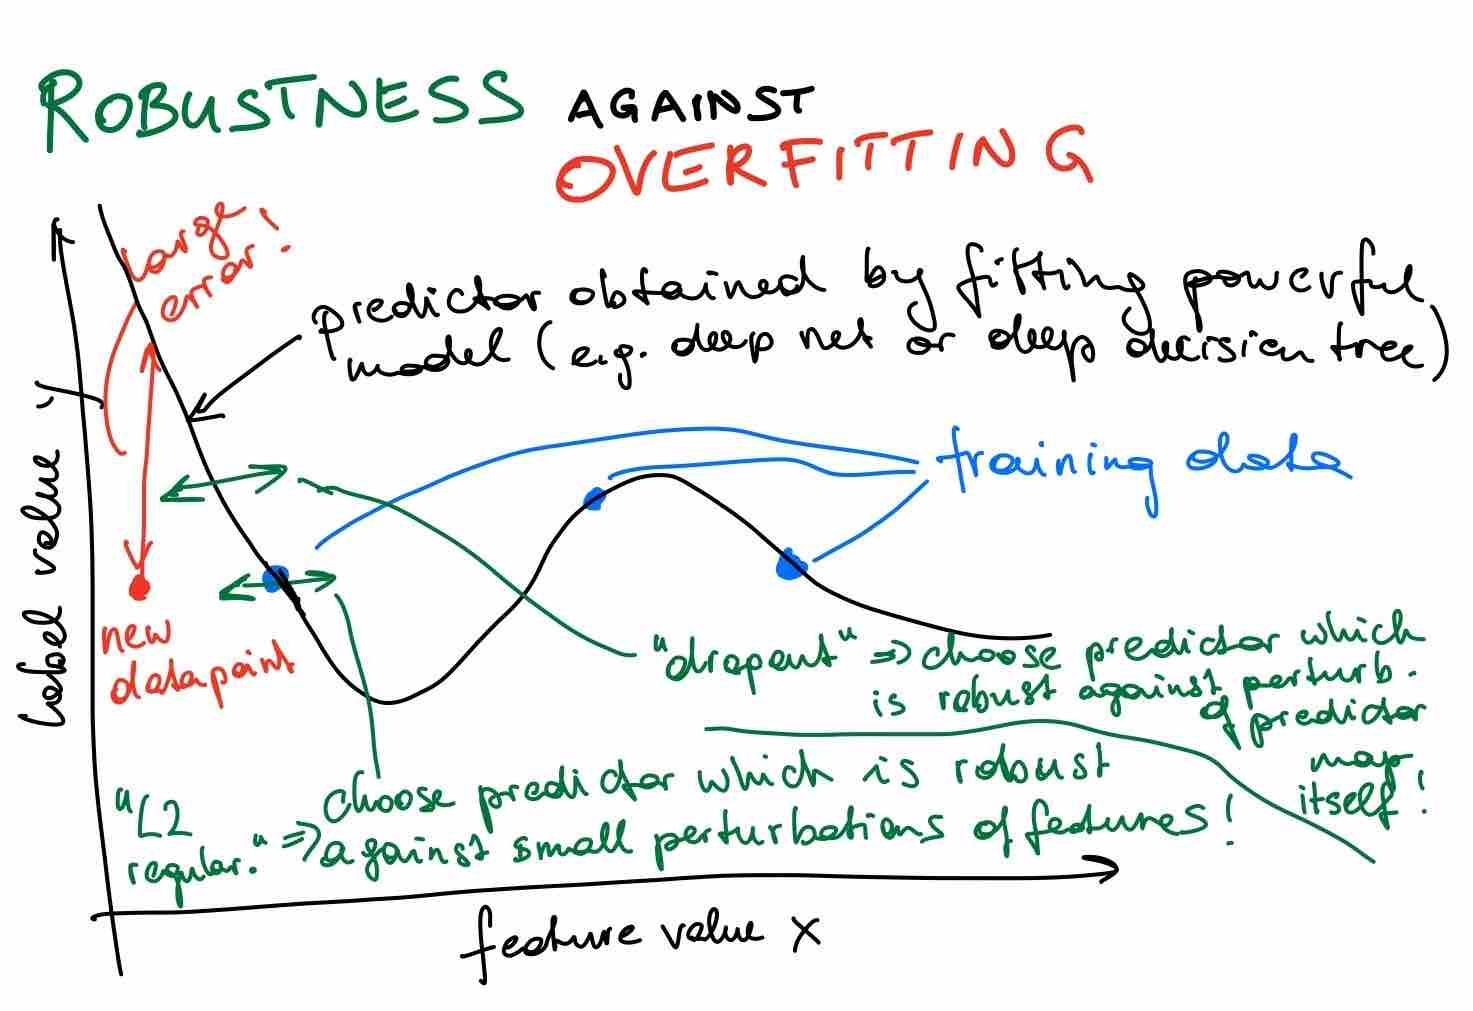
\includegraphics[width=\textwidth]{RobustnessOverfitting.jpg}  
	\caption{Modern ML methods allow to find a predictor map that perfectly fits 
		training data. Such a predictor might perform poorly on a new datapoint 
		outside the training set. To prevent learning such a predictor 
		map we could require it to be robust against small perturbations in the features of the 
        training datapoints or the predictor map itself.}
	\label{fig_polyn_training}
\end{figure}

\section{Data Augmentation} 
\label{sec_data_augmentation} 
implement robustness principle by augmenting dataset with random perturbations of original training data. 

ML methods using ERM \eqref{equ_def_ERM_funs} are prone to overfitting as soon 
as the effective dimension of the hypothesis space $\hypospace$ exceeds the number 
$\samplesize$ of training datapoints. Section \ref{sec_modsel} and Section \ref{sec_reg_ERM} 
approached this by modifying either the model or the loss function. We can also approach 
this via somehow enlarging the dataset. 

The data arising in many ML applications exhibit intrinsic symmetries and invariances at least in 
some approximation. The rotated image of a cat still shows a cat. The temperature measurement 
taken at a given location will be similar to another measurement taken $10$ milliseconds later. 
Data augmentation exploits such symmetries and invariances to augment the raw data with 
additional synthetic data. 

Let us illustrate data augmentation using an application that involves data points characterized 
by features $\vx \in \mathbb{R}^{\featuredim}$ and number labels $y \in \mathbb{R}$. We assume 
that the data generating process is such that data points with close feature values have the same label. 
This suggests to augment a data point $\big(\vx,y\big)$ by several synthetic data points 
\begin{equation} 
\label{equ_def_copies_aug}
\big(\vx+{\bm \varepsilon}^{(1)},y\big),\ldots,\big(\vx+{\bm \varepsilon}^{(\augparam)},y\big), 
\end{equation}
with ${\bm \varepsilon}^{(1)},\ldots,{\bm \varepsilon}^{(\augparam)}$ being realizations of i.i.d. 
random vectors with the same probability distribution $p(\vu)$. 

Given a (raw) dataset $\dataset = \big\{ \big(\vx^{(1)},y^{(1)}\big),\ldots, \big(\vx^{(\samplesize)},y^{(\samplesize)}\big) \} $ 
we denote the associated augmented dataset by 
\begin{align} 
\label{equ_def_augmented_dataset}
\dataset' = \big\{ &\big(\vx^{(1,1)},y^{(1)}\big), \ldots, \big(\vx^{(1,\augparam)},y^{(1)}\big), \nonumber \\ 
                                  &\big(\vx^{(2,1)},y^{(2)}\big), \ldots, \big(\vx^{(2,B)},y^{(2)}\big), \nonumber \\ 
                                  & \ldots \nonumber \\ 
 &\big(\vx^{(\samplesize,1)},y^{(\samplesize)}\big), \ldots, \big(\vx^{(\samplesize,\augparam)},y^{(\samplesize)}\big) \}. 
\end{align} 
The size of the augmented dataset $\dataset'$ is $ \samplesize' = \augparam \times \samplesize$. 
For a sufficiently large augmentation parameter $\augparam$, the augmented samplesize $\samplesize'$ is 
larger than the effective dimension $\featurelen$ of the hypothesis space $\hypospace$. We might 
then learn a hypothesis by ERM on the augmented dataset, 
\begin{align}
\label{equ_def_ERM_funs_aug}
\hat{h} & = \argmin_{h \in \hypospace} \emperror(h|\dataset') \nonumber \\ 
& \stackrel{\eqref{equ_def_augmented_dataset}}{=}  \argmin_{h \in \hypospace} (1/\samplesize') \sum_{\sampleidx=1}^{\samplesize} \sum_{b=1}^{B} \loss{(\vx^{(\sampleidx,b)},y^{(\sampleidx,b)})}{h} \nonumber \\ 
& \stackrel{\eqref{equ_def_copies_aug}}{=}  \argmin_{h \in \hypospace} (1/\samplesize) \sum_{\sampleidx=1}^{\samplesize} (1/\augparam)\sum_{b=1}^{\augparam} \loss{(\vx^{(\sampleidx)}+{\bm \varepsilon}^{(b)},y^{(\sampleidx)})}{h}. 
\end{align}
We can interpret data-augmented ERM \eqref{equ_def_ERM_funs_aug} as a data-driven 
form of regularization (see Section \ref{sec_reg_ERM}). The regularization is implemented 
by replacing the loss $\loss{(\vx^{(\sampleidx)},y^{(\sampleidx)})}{h}$ incurred for the 
datapoint $(\vx^{(\sampleidx)},y^{(\sampleidx)})$ with the average 
loss $(1/\augparam)\sum_{b=1}^{\augparam} \loss{(\vx^{(\sampleidx)}+{\bm \varepsilon}^{(b)},y^{(\sampleidx)})}{h}$ 
incurred over the augmented datapoints. 

Note that in order to implement \eqref{equ_def_ERM_funs_aug} we need to first generate 
$\augparam$ realizations  ${\bm \varepsilon}^{(b)} \in \mathbb{R}^{\featurelen}$ of i.i.d.
random vectors with probability distribution $p(\vu)$. 
This might be computationally costly for a large $\augparam, \featurelen$. 
However, when using a large augmentation parameter $\augparam$, we might 
use the approximation  
\begin{align}
\label{equ_approx_augm_loss_expect}
 (1/\augparam)\sum_{b=1}^{\augparam} \loss{(\vx^{(\sampleidx)}+{\bm \varepsilon}^{(b)},y^{(\sampleidx)})}{h} \approx  
 \expect_{{\bm \varepsilon} \sim p(\vu) } \big\{ \loss{(\vx^{(\sampleidx)}+{\bm \varepsilon},y^{(\sampleidx)})}{h} \big\}. 
\end{align}
This approximation is made precise by a key result of probability theory, known as the law of large numbers. 

We can learn a hypothesis by inserting \eqref{equ_approx_augm_loss_expect} into \eqref{equ_def_ERM_funs_aug}, 
\begin{align}
\label{equ_def_ERM_funs_aug_approx}
\hat{h}  = \argmin_{h \in \hypospace} (1/\samplesize) \sum_{\sampleidx=1}^{\samplesize} \expect_{{\bm \varepsilon} \sim p(\vu) } \big\{ \loss{(\vx^{(\sampleidx)}+{\bm \varepsilon},y^{(\sampleidx)})}{h} \big\}. 
\end{align}


The usefulness of \eqref{equ_def_ERM_funs_aug_approx} as a computationally efficient approximation to 
the augmented ERM \eqref{equ_def_ERM_funs_aug} depends on the complexity of computing the 
expectation $\expect_{{\bm \varepsilon} \sim p(\vu) } \big\{ \loss{(\vx^{(\sampleidx)}+{\bm \varepsilon},y^{(\sampleidx)})}{h} \big\}$. 
The complexity of computing this expectation depends on the choice of loss function and the 
choice for the probability distribution $p(\vu)$.  

Let us evaluate \eqref{equ_def_ERM_funs_aug_approx} for the special case of squared error loss \eqref{equ_squared_loss} 
and $p(\vu)$ being a multivariate normal distribution with zero mean and covariance matrix $\sigma^{2} \mathbf{I}$. Using 
basic calculus of probability theory, 
 \begin{align} 
 \label{equ_implicit_aug_regu_1}
 \expect_{{\bm \varepsilon} \sim p(\vu) } \big\{ \loss{(\vx^{(\sampleidx)}+{\bm \varepsilon},y^{(\sampleidx)})}{h^{(\vw)}} \big\} & \stackrel{\eqref{equ_squared_loss}}{=}
  \expect_{{\bm \varepsilon} \sim p(\vu) } \big( y^{(\sampleidx)} - h^{(\vw)} \big(\vx^{(\sampleidx)}+{\bm \varepsilon} \big)\big)^{2}  \nonumber \\
  & \stackrel{h^{(\vw)}(\vx) = \vw^{T} \vx}{=}  \expect_{{\bm \varepsilon} \sim p(\vu) }\big( y^{(\sampleidx)} - \vw^{T} \big(\vx^{(\sampleidx)}+{\bm \varepsilon} \big) \big)^{2}.
\end{align}

We can develop \eqref{equ_implicit_aug_regu_1} further by using 
\begin{equation} 
\label{equ_uncorr_augmentation_implicit}
\expect\{\big( y^{(\sampleidx)} - \vw^{T} \vx^{(\sampleidx)} \big) {\bm \varepsilon}  \} = \mathbf{0},
\end{equation}
which follows from our assumption that the datapoints $\big(\vx^{(\sampleidx)},y^{(\sampleidx)}$ are 
fixed and known (deterministic) while ${\bm \varepsilon}$ is a zero-mean random vector.
Inserting \eqref{equ_uncorr_augmentation_implicit} into \eqref{equ_implicit_aug_regu_1}, 
 \begin{align} 
\label{equ_implicit_aug_regu_11}
\expect_{{\bm \varepsilon} \sim p(\vu) } \big\{ \loss{(\vx^{(\sampleidx)}+{\bm \varepsilon},y^{(\sampleidx)})}{h^{(\vw)}} \big\} 
& \stackrel{\eqref{equ_uncorr_augmentation_implicit},\eqref{equ_implicit_aug_regu_1}}{=}  
\expect_{{\bm \varepsilon} \sim p(\vu) }\big[ \big( y^{(\sampleidx)} - \vw^{T}\vx^{(\sampleidx)} \big) ^{2} 
\!+\!\big\| \vw \big\|^{2} \big\| {\bm \varepsilon} \big\|^{2}\big] \nonumber \\ 
& = \big( y^{(\sampleidx)} - \vw^{T}\vx^{(\sampleidx)} \big) ^{2} \!+\!\big\| \vw \big\|^{2}  \expect_{{\bm \varepsilon} \sim p(\vu) }  \big\| {\bm \varepsilon} \big\|^{2}, 
\end{align}
where the last step used the linearity of expectations. Since the covariance matrix of ${\bm \varepsilon}$ is 
$\sigma^{2} \mathbf{I}$, i.e., $\expect_{{\bm \varepsilon} \sim p(\vu) }  \big\| {\bm \varepsilon} \big\|^{2} = \featurelen \sigma^{2}$, 
 \begin{align} 
\label{equ_implicit_aug_regu_111}
\expect_{{\bm \varepsilon} \sim p(\vu) } \big\{ \loss{(\vx^{(\sampleidx)}+{\bm \varepsilon},y^{(\sampleidx)})}{h^{(\vw)}} \big\} 
& = \big( y^{(\sampleidx)} - \vw^{T}\vx^{(\sampleidx)} \big) ^{2}  + \featurelen \big\| \vw \big\|^{2}  \sigma^{2}. 
\end{align}

Inserting \eqref{equ_implicit_aug_regu_111} into \eqref{equ_def_ERM_funs_aug_approx}, 
\begin{align}
\label{equ_def_ERM_funs_aug_approx_ridge}
\hat{h}  = \argmin_{h \in \hypospace} (1/\samplesize) \sum_{\sampleidx=1}^{\samplesize} \big( y^{(\sampleidx)} - \vw^{T}\vx^{(\sampleidx)} \big) ^{2}  + \featurelen \big\| \vw \big\|^{2}  \sigma^{2}.
\end{align}
We have obtained \eqref{equ_def_ERM_funs_aug_approx_ridge} as an approximation of 
the augmented ERM \eqref{equ_def_ERM_funs_aug} for the special case of squared error 
loss and linear hypotheses. This approximation uses the law of large numbers \eqref{equ_approx_augm_loss_expect} 
and becomes more accurate for increasing augmentation parameter $\augparam$. 

We emphasize that \eqref{equ_def_ERM_funs_aug_approx_ridge} is nothing but ridge regression 
\eqref{equ_rerm_ridge_regression} using the regularization parameter $\lambda  =\featurelen \sigma^{2}$. 
Thus, we can interpret ridge regression as using an implicit data augmentation \eqref{equ_def_augmented_dataset} 
using random perturbations \eqref{equ_def_copies_aug} of the feature vectors of raw datapoint (while leaving their 
labels untouched). 

Note that the regularizer $\mathcal{R}(\vw) = \| \vw \|^{2}$ in \eqref{equ_def_ERM_funs_aug_approx_ridge} 
arose naturally from the specific choice for the probability distribution $p(\vu)$ of the random perturbation ${\bm \varepsilon}^{(\sampleidx)}$ 
in \eqref{equ_def_copies_aug} and using the squared error loss. Other choices for this probability distribution or the 
loss function result in different regularizers. 





  

 







\section{A Probabilistic Analysis of Regularization}
\label{sec_prob_mod_regularization}

Specialising \eqref{equ_rerm} to the squared error loss and linear predictors 
yields {\bf regularized linear regression} (see \eqref{equ_def_cost_MSE}): 
\begin{equation} 
\label{equ_reg_lin_reg_opt_weight}
\hat{\vw}^{(\lambda)} = \argmin_{\vw \in \mathbb{R}^{\featuredim}} \big[ (1/\samplesize_{\rm t}) \sum_{\sampleidx=1}^{\samplesize_{\rm t}}  (y^{(\sampleidx)} - \vw^{T}\vx^{(\sampleidx)}  )^2 + \lambda \| \vw \|^{2}_{2}\big], 
\end{equation} 
The optimization problem \eqref{equ_reg_lin_reg_opt_weight} is also known 
under the name {\bf ridge regression} \cite{hastie01statisticallearning}. 

%?????
%It is interesting to note that ridge regression \eqref{equ_reg_lin_reg_opt_weight} arises naturally as the optimal Bayes estimator of the weight vector $\vw$ if it is modeled 
%as a Gaussian random vector $\vw \sim \mathcal{N}(\mathbf{0},\sigma_{w}^{2} \mathbf{I}$ etcetcetc. Moreover, the ridge regression problem \eqref{equ_reg_lin_reg_opt_weight} 
%turns out to be almost optimal in terms of minimizing the ???regret??? when implemented as an online learning method \cite[Ch. 11]{PredictionLearningGames}
%MAYBE discuss online learning interpretation of ridge regression in a new section "Online Learning" which comes after Chapter 7 
%??????

Using the feature matrix $\mX=\big(\vx^{(1)},\ldots,\vx^{(\samplesize_{\rm t})}\big)^{T}$ 
and label vector $\vy=(y^{(1)},\ldots,y^{(\samplesize_{\rm t})})^{T}$, 
we can rewrite \eqref{equ_reg_lin_reg_opt_weight} more compactly as 
\begin{equation} 
\label{equ_def_rlr_w_opt}
\hat{\vw}^{(\lambda)} = \argmin_{\vw \in \mathbb{R}^{\featuredim}} \big[ (1/\samplesize_{\rm t}) \| \vy - \mX \vw \|^{2}_{2} + \lambda \| \vw \|^{2}_{2}\big].
\end{equation} 
The solution of \eqref{equ_def_rlr_w_opt} is given by 
\begin{equation}
\label{equ_close_form_reglinreg}
\hat{\vw}^{(\lambda)} = (1/\samplesize_{\rm t}) ((1/\samplesize_{\rm t}) \mX^{T} \mX + \lambda \mathbf{I})^{-1} \mX^{T} \vy. 
\end{equation}
This reduces to the closed-form expression \eqref{equ_optimal_weight_closed_form} 
when $\lambda=0$ in which case regularized linear regression reduces to ordinary linear 
regression (see \eqref{equ_reg_lin_reg_opt_weight} and \eqref{equ_def_cost_MSE}). It 
is important to note that for $\lambda>0$, the formula \eqref{equ_close_form_reglinreg} 
is always valid, even when $\mX^{T} \mX$ is singular (not invertible). This implies, in turn, 
that for $\lambda> 0$ the optimization problem \eqref{equ_def_rlr_w_opt} (and \eqref{equ_reg_lin_reg_opt_weight}) 
has a unique solution (which is given by \eqref{equ_close_form_reglinreg}). 

We now study the effect of regularization on the bias, variance 
and average prediction error incurred by the predictor $h^{(\hat{\vw}^{(\lambda)})}(\vx) = \big(\hat{\vw}^{(\lambda)}\big)^{T} \vx$. 
To this end, we will again invoke the simple probabilistic toy 
model (see \eqref{equ_linear_obs_model}, \eqref{equ_toy_model_iid} 
and \eqref{equ_labels_training_data}) used already in Section \ref{sec_gen_linreg}. 
In particular, we interpret the training data $\dataset^{(\rm train)} = \{ (\vx^{(\sampleidx)},y^{(\sampleidx)}) \}_{\sampleidx=1}^{\samplesize_{\rm t}}$ 
as realizations of i.i.d.\ random variables according to \eqref{equ_linear_obs_model}, 
\eqref{equ_toy_model_iid} and \eqref{equ_labels_training_data}. 
%We aim at predicting the label $y$ based on the first $r$ entries of the feature vector $\vx$ (see \eqref{equ_generalization_hypospace_r}). 

As discussed in Section \ref{sec_gen_linreg}, the average prediction 
error is the sum of three components: the bias, the variance and the 
noise variance $\sigma^{2}$ (see \eqref{equ_decomp_E_pred_toy_model}). 
The bias of regularized linear regression \eqref{equ_reg_lin_reg_opt_weight} 
is obtained as 
\begin{equation} 
\label{equ_bias_reg_lin_reg}
B^{2} = \big \| (\mathbf{I} - \expect \{ ( \mX^{T} \mX +  \samplesize \lambda \mathbf{I})^{-1} \mX^{T} \mX  \})  \bar{\vw} \big  \|^{2}_{2}. 
%B^{2} =    \| (\mathbf{I}-\mX_{r}^{T} \mX_{r} ) \mathbf{I}_{r \times \featuredim} \vw_{\rm true} \}   \} \|^{2}_{2} \geq \sum_{l=r+1}^{\featuredim} w_{{\rm true},l}^2  
\end{equation} 
For sufficiently large sample size $\samplesize_{\rm t}$ we can use the approximation 
\begin{equation} 
\label{equ_approx_Gram_large_N}
\mX^{T} \mX  \approx \samplesize_{\rm t} \mathbf{I} 
\end{equation} 
such that \eqref{equ_bias_reg_lin_reg} can be approximated as 
 \begin{align} 
\label{equ_bias_reg_lin_reg_approx}
B^{2} & \approx \big \| (\mathbf{I}\!-\!(\mathbf{I}\!+\!\lambda \mathbf{I})^{-1} ) \bar{\vw} \big  \|^{2}_{2} \nonumber \\
& =  \sum_{l=1}^{\featuredim} \frac{\lambda}{1+\lambda} \bar{w}_{l}^2 .
\end{align} 
Compare the (approximate) bias term \eqref{equ_bias_reg_lin_reg_approx} 
of regularized linear regression with the bias term \eqref{equ_def_bias_term} of 
ordinary linear regression. Using regularization typically increases the bias. 
The bias increases with increasing regularization parameter $\lambda$. 

The variance of regularized linear regression \eqref{equ_reg_lin_reg_opt_weight} satisfies 
\begin{align}
\label{equ_variance_reglinreg}
V & =( \sigma^{2}/\samplesize^{2}_{\rm t}) \times \nonumber \\ 
& \hspace*{-7mm} {\rm tr} \big\{  \expect \{  ( (1/\samplesize_{\rm t}) \mX^{T} \mX\!+\!\lambda \mathbf{I} )^{-1} \mX^{T} \mX ( (1/\samplesize_{\rm t}) \mX^{T} \mX\!+\!\lambda \mathbf{I} )^{-1}   \} \big\}.
\end{align}
%The approximation \eqref{equ_approx_Gram_large_N} becomes more accurate with 
%increasing sample size $\samplesize_{\rm t}$. 
Inserting the approximation \eqref{equ_approx_Gram_large_N} into \eqref{equ_variance_reglinreg},  
\begin{equation}
\label{equ_variance_reglinreg_approx}
V \approx \sigma^{2} (\featuredim/\samplesize_{\rm t}) (1/(1+ \lambda)).
\end{equation} 
According to \eqref{equ_variance_reglinreg_approx}, the variance of regularized linear 
regression decreases with increasing regularization parameter $\lambda$. This is the 
opposite behaviour as for the bias \eqref{equ_bias_reg_lin_reg_approx}, which increases 
with increasing $\lambda$. 

Figure \ref{fig_bias_variance_lambda} illustrates a trade-off between the bias $B^{2}$ 
\eqref{equ_bias_reg_lin_reg_approx}, which increases for increasing $\lambda$, 
and the variance $V$ \eqref{equ_variance_reglinreg_approx} which decreases with increasing $\lambda$.
We have discussed another example for a bias-variance trade-off already in Section \ref{sec_gen_linreg}. 
In contrast to the trade-off obtained there for the discrete model complexity $r$ in \eqref{equ_generalization_hypospace_r}, 
here we obtain a continuous trade-off via the real-valued parameter $\lambda$. 


\begin{figure}
\begin{center}
    \begin{tikzpicture}
              \draw [thick, <->] (0,3.5) -- (0,0) -- (6.2,0);
             \draw[red, ultra thick, domain=0:5] plot (\x,  {2*\x/(1+\x)}) node [above] {bias of $\hat{\vw}^{(\lambda)}$};
              \draw[blue, ultra thick, domain=0:5] plot (\x,  {2/(1+\x)}) node [above]  {variance of $\hat{\vw}^{(\lambda)}$};
              \node [below] at (5,0) {regularization parameter $\lambda$};
     \end{tikzpicture}
\end{center}
\caption{The bias and variance of regularized linear regression depend on the regularization parameter 
$\lambda$ in an opposite manner resulting in a bias-variance tradeoff.}
\label{fig_bias_variance_lambda}
\end{figure}

%???? 
%Choice of lambda can be guided by validation error 
%???????

So far, we only have discussed the statistical effect of regularization on the 
resulting ML method. Regularizations allows to trade off bias against variance 
in order to reduce the risk of the learnt hypothesis. 

There is also a computational aspect of regularization. Adding a regularization 
term to the ERM changes the shape of the objective function that is minimized 
by a learning method. The shape of the objective function determines the difficulty 
in finding a (approximate) minimizer. Thus, regularization influences the computational
complexity of the resulting ML method.  

Note that the objective function in \eqref{equ_def_rlr_w_opt} is a smooth (infinitely often differentiable) 
convex function. Similar to linear regression, we can solve the regularization 
linear regression problem using GD \eqref{equ_squared_loss} 
(see Algorithm \ref{alg:gd_reglinreg}). 

Adding the regularization term $\lambda \| \vw \|^{2}_{2}$ to the objective 
function of linear regression {\bf speeds up GD}. To verify this claim, we first 
rewrite \eqref{equ_def_rlr_w_opt} as the quadratic problem 
\begin{align} 
\label{equ_quadr_form_reglinreg}
\min_{\vw \in \mathbb{R}^{\featuredim}} & \underbrace{(1/2) \vw^{T} \mQ \vw - \vq^{T}  \vw}_{= f(\vw)} \nonumber \\ 
 & \mbox{ with } \mathbf{Q}= (1/\samplesize) \mX^{T} \mX + \lambda \mathbf{I}, \vq =(1/\samplesize) \mX^{T} \vy. %\mathbf{X}^{T} 
%\min_{\mathbf{w} \in \mathbb{R}^{\featuredim}} \mathbf{w}^{T} \mathbf{Q} \mathbf{w}  \mbox{, with } \mathbf{Q} = \mathbf{X}^{T} \mathbf{X} + \lambda \mathbf{I}.
\end{align} 
This is similar to the quadratic optimization problem \eqref{equ_quadr_form_linreg} 
underlying linear regression but with a different matrix $\mQ$. It turns out 
that the convergence speed of GD (see \eqref{equ_def_GD_step}) applied 
to solving a quadratic problem of the form \eqref{equ_quadr_form_reglinreg} 
depends crucially on the condition number $\kappa(\mQ) \geq 1$ of the 
psd matrix $\mQ$ \cite{JungFixedPoint}. In particular, GD methods are fast 
if the condition number $\kappa(\mQ)$ is small (close to $1$). 

This condition number is given by $\frac{\lambda_{\rm max}((1/\samplesize) \mX^{T} \mX)} {\lambda_{\rm min}((1/\samplesize) \mX^{T} \mX)}$ for ordinary linear regression 
(see \eqref{equ_quadr_form_linreg}) and given by $\frac{\lambda_{\rm max}((1/\samplesize)\mX^{T} \mX) + \lambda} {\lambda_{\rm min}((1/\samplesize)\mX^{T} \mX)+ \lambda}$ 
for regularized linear regression \eqref{equ_quadr_form_reglinreg}. For increasing 
regularization parameter $\lambda$, the condition number obtained for regularized 
linear regression \eqref{equ_quadr_form_reglinreg} tends to approach $1$, 
\begin{equation}
\label{equ_cond_numer_goes_1_rlr}
\lim_{\lambda \rightarrow \infty} \frac{\lambda_{\rm max}((1/\samplesize)\mX^{T} \mX) + \lambda} {\lambda_{\rm min}((1/\samplesize)\mX^{T} \mX)+ \lambda} =1. 
\end{equation} 
According to \eqref{equ_cond_numer_goes_1_rlr}, the GD 
implementation of regularized linear regression (see Algorithm \ref{alg:gd_reglinreg}) 
with a large value of the regularization parameter $\lambda$ 
in \eqref{equ_reg_lin_reg_opt_weight} will converge faster compared 
to GD for linear regression (see Algorithm \ref{alg:gd_linreg}). 


\begin{algorithm}[htbp]
\caption{``Regularized Linear Regression via GD''}\label{alg:gd_reglinreg}
\begin{algorithmic}[1]
\renewcommand{\algorithmicrequire}{\textbf{Input:}}
\renewcommand{\algorithmicensure}{\textbf{Output:}}
\Require   labeled dataset $\dataset=\{ (\vx^{(\sampleidx)}, y^{(\sampleidx)}) \}_{\sampleidx=1}^{\samplesize}$ containing feature vectors 
$\vx^{(\sampleidx)} \in \mathbb{R}^{\featuredim}$ and labels $y^{(\sampleidx)} \in \mathbb{R}$; GD step size $\alpha >0$. 
\Statex\hspace{-6mm}{\bf Initialize:}set $\vw^{(0)}\!\defeq\!\mathbf{0}$; set iteration counter $k\!\defeq\!0$   
\Repeat 
\State $k \defeq k +1$    (increase iteration counter) 
\State  $\vw^{(k)} \defeq (1- \alpha \lambda) \vw^{(k\!-\!1)} + \alpha (2/\samplesize) \sum_{\sampleidx=1}^{\samplesize} (y^{(\sampleidx)} - \big(\vw^{(k\!-\!1)})^{T} \vx^{(\sampleidx)}) \vx^{(\sampleidx)}$  (do a GD step \eqref{equ_def_GD_step})
\Until convergence 
\Ensure $\vw^{(k)}$ (which approximates $\hat{\vw}^{(\lambda)}$ in \eqref{equ_def_rlr_w_opt})
\end{algorithmic}
\end{algorithm}

Let us finally point out a close relation between regularization (which amounts to 
adding the term $\lambda \| \vw \|^{2}$ to the objective function in \eqref{equ_rerm}) 
and model selection (see Section \ref{sec_modsel}). The regularized ERM \eqref{equ_rerm} 
can be shown (see \cite[Ch. 5]{BertsekasNonLinProgr}) to be equivalent to 
\begin{equation} 
\label{equ_restr_ERM}
\hat{\vw}^{(\lambda)} = \argmin_{h^{(\vw)} \in \hypospace^{(\lambda)}}  (1/m_{\rm t}) \sum_{\sampleidx=1}^{\samplesize_{\rm t}}  (y^{(\sampleidx)} - h^{(\vw)}(\vx^{(\sampleidx)})  )^2
\end{equation}  
with the restricted hypothesis space
\begin{align} 
\label{equ_hyposapce_lambda}
\hypospace^{(\lambda)} & \defeq \{ h^{(\vw)}: \mathbb{R}^{\featuredim} \rightarrow \mathbb{R}: h^{(\vw)}(\vx) = \vw^{T} \vx \nonumber \\
& \mbox{, with some } \vw \mbox{ satisfying } \| \vw \|^{2} \leq C(\lambda) \} \subset \hypospace^{(\featuredim)}. 
\end{align} 
For any given value $\lambda$, there is a $C(\lambda)$ such that 
solutions of \eqref{equ_rerm} coincide with the solutions of \eqref{equ_restr_ERM}. 
We can interpret regularized ERM \eqref{equ_rerm} as a form of model selection using 
a continuous ensemble of hypothesis spaces $\hypospace^{(\lambda)}$ \eqref{equ_hyposapce_lambda}. 
In contrast, the simple model selection strategy considered in Section \ref{sec_modsel} 
uses a discrete sequence of hypothesis spaces.   

%\subsection{How To Choose $\lambda$?} 
%????
%Using a validation set. Given a finite set of candidate values of lambda, compute the val error of those 
%candidates and pick the best. Why not pushing this further and derive a close-form expression for val error (for a fixed particular val set!) 
%and then minimize this expression? --> by cannot test too many values of lambda due to limited information content in one particular val set (related to uniform convergence principle) 
%---> moreover, we are not interested in optimal val error for one fixed val set but in an average val error (=generalization error). 
%?????
%Can we use closed form experessions for bias and variance obtained for our toy model ? In general, not possible since bias 
%depends on unknown true weight vector. However, we might have some partial information about weight vector (belongs to some convex set) which 
%would allow to get some idea (minimax?) of how to choose $\lambda$ 
%????????
%???????
%The SURE depends solely on y, without prior knowledge of x0. This can prove very useful as a basis to automatically choose the parameters ? of the estimator, e.g. ? = ? when solving (2), or the smoothing parameters in families of linear estimates [28] such as for ridge regression or smoothing splines. In some settings, it has been shown that it offers better accuracy than GCV and related non-parametric selection techniques [29]. However, compared to GCV, the SURE requires the knowledge of the noise variance ?2  see \url{https://arxiv.org/pdf/1204.3212.pdf}
%??????

\section{Semi-Supervised Learning} 
\label{sec_ssl_regularization}
%%% use unlabeled data to construct regularizers ?? 
Can we use unlabelled datapoints to construct better regularizers? We could use unlabled data 
to learn some subspace of features that are most relevant ? (relation to feature learning ?)

\section{Multitask Learning} 
\label{sec_mtl_regularization}
%%%% use different tasks to construct regularizers ????
Remember that a formal ML problem is specified by identifying 
datapoints, their features and labels, a model (hypothesis space)
and a loss function. Note that we can use the very same raw data, model 
and loss function and still define many different ML problems by 
using different choices for the label. Multitask learning aims at 
exploiting relations between similar ML problems or tasks. 

Consider the ML problem (task) of predicting the confidence level 
of a hand-drawing showing an apple. To learn such a predictor we 
use a collection of hand-drawings. We then annotate each hand-drawing 
by the object that it depicts. These annotations can be used to define 
different labels of the hand-drawings. One choice for the label could 
be to define the label $y=1$ if a hand-drawing shows an apple and 
$y=0$ if it does not show a hand-drawing. Another definition for 
the label could be based on the fact that the hand-drawing shows 
an apple or not. 


Different choices for the label result in different ML problems. These 
different ML problems are related since they are based on the same data 
points, the hand-drawings. Some ML problems (label choices) are more 
difficult to solve while others are easier to solve. 

One important criterion for the difficulty in solving a particular ML problem 
is the availability of labeled datapoints. For some choices for the labels, we 
might have no labeled datapoints available. Consider datapoints representing 
different days in Finland. It might be easy to get labeled datapoints when the 
label of a datapoint is the minimum daytime temperature measured at some 
observation station of FMI. If we would use instead as the label the precise 
water temperature at some remote lake (not having any sensors), we would 
not have access to any labeled datapoint. 


Consider the ML problem arising from guiding the operation of a mower robot. 
For a mowing robot, it is important to determine if it is currently on grassland 
or not. Let us assume the mower robot is equipped with an on-board camera 
which allows to take snapshots which are characterized by a feature vector 
$\mathbf{x}$ (see Figure \ref{fig_snapshot_pixels}). We could then define the 
label as either $y=1$ if the snapshot suggests that the mower is on grassland 
and $y=-1$ if not. However, we might be interested in a finer-grained information 
about the floor type and define the label as $y=1$ for grassland, 
$y=0$ for soil and $y=-1$ for when the mower is on tiles. The latter problem is 
more difficult since we have to distinguish between three different types of 
floor (``grass'' vs. ``soil'' vs. ``tiles'') whereas for the former problem we only 
have to distinguish between two types of floor (``grass'' vs. ``no grass''). 


\section{Exercises} 
\subsection{Ridge Regression as Quadratic Form} 
\label{ex_2_0}
Consider linear hypothesis space consisting of linear maps parameterized by 
weights $\mathbf{w}$. We try to find the best linear map by minimizing the regularized average 
squared error loss (empirical risk) incurred on some labeled training datapoints 
$(\vx^{(1)},y^{(1)}),(\vx^{(2)},y^{(2)}),\ldots,(\vx^{(\samplesize)},y^{(\samplesize)})$. 
As regularizer we use $\| \mathbf{w} \|^{2}$, yielding the following learning problem 
$$ \min_{\vw} f(\vw) = \sum_{i=1}^{\samplesize}\ldots + \| \mathbf{w} \|^{2}_{2}.$$

Is it possible to write the objective function $f(\vw)$ as a convex quadratic form 
$f(\vw) = \vw^{T} \mathbf{C} \vw + \vb \vw + c$? If this is possible, how are the 
matrix $\mathbf{C}$, vector $\vb$ and constant $c$ related to the feature vectors 
and labels of the training data ? 

\subsection{Regularization or Model Selection} 
Consider datapoints characterized by $\featurelen=10$ features $\vx \in \mathbb{R}^{\featurelen}$ 
and a single numeric label $y$. We want to learn a linear hypothesis $h(x) = \vw^{T} \vx$ by 
minimizing the average squared error on the training set $\dataset$ of size $\samplesize=4$. 
We could learn such a hypothesis by two approaches. The first approach is split the dataset 
into training and validation set of the same size (two). Then we consider all models that are given by 
linear hypothesis with weight vectors have at most two non-zeros. We use the validation 
set to choose between these models. The second approach is learn a linear hypothesis 
with arbitrary weight vector $\vw$ but using regularization (ridge). 



\newpage
\chapter{Clustering} 
\label{ch_Clustering}



\begin{figure}[htbp]
\begin{center}
\begin{tikzpicture}[auto,scale=0.8]
\draw [thick] (5,2.5) circle (0.1cm)node[anchor=west] {\hspace*{0mm}$\vx^{(3)}$};
\draw [thick] (4,2) circle (0.1cm)node[anchor=west] {\hspace*{0mm}$\vx^{(4)}$};
\draw [thick] (5,1) circle (0.1cm)node[anchor=west,above] {\hspace*{0mm}$\vx^{(2)}$};
\draw [thick] (1,5) rectangle ++(0.1cm,0.1cm) node[anchor=west,above] {\hspace*{0mm}$\vx^{(1)}$};
\draw [thick] (1,3.5) rectangle ++(0.1cm,0.1cm) node[anchor=west,above] {\hspace*{0mm}$\vx^{(5)}$};
\draw [thick] (1,2.5) rectangle ++(0.1cm,0.1cm) node[anchor=west,above] {\hspace*{0mm}$\vx^{(6)}$};
\draw [thick] (2,4) rectangle ++(0.1cm,0.1cm) node[anchor=west,above] {\hspace*{0mm}$\vx^{(7)}$};
\draw[->] (-0.5,0) -- (6.5,0) node[right] {$x_{\rm g}$};
\draw[->] (0,-0.5) -- (0,6.5) node[above] {$x_{\rm r}$};
%\foreach \y/\ytext in { 1/1,2/2,3/3,4/4,5/5} \draw[shift={(0,\y)}] (2pt,0pt) -- (-2pt,0pt) node[left] {$\ytext/5$};  
%\foreach \x/\xtext in{ 1/1,2/2,3/3,4/4,5/5}\draw[shift={(\x,0)}] (0pt,2pt) -- (0pt,-2pt) node[below] {$\xtext/5$};  
\end{tikzpicture}
\end{center}
\caption{A scatterplot depicting some images. The $\sampleidx$-th image is 
	represented by the feature vector $\vx^{(\sampleidx)}=(x^{(\sampleidx)}_{\rm r},x^{(\sampleidx)}_{\rm g})^{T}$ 
	with the average redness $x_{\rm r}^{(\sampleidx)}$ and average greenness $x_{\rm g}^{(\sampleidx)}$ of the image. 
} 
\label{fig_scatterplot_clustering}
\end{figure}

Up to now, we mainly considered ML methods which required 
some labeled training data in order to learn a good predictor or 
classifier. We will now start to discuss ML methods which do 
not make use of labels. These methods are often referred to as 
``unsupervised'' since they do not require a supervisor 
(or teacher) which provides the labels for datapoints in a training set. 

An important class of unsupervised methods, known as clustering 
methods, aims at grouping datapoints into few subsets (or {\bf clusters}). 
While there is no unique formal definition, we understand by cluster 
a subset of datapoints which are more similar to each other than 
to the remaining datapoints (belonging to different clusters). Different 
clustering methods are obtained for different ways to measure the 
``similarity'' between datapoints. 

%
%Consider the scatter plot in Figure \ref{fig_scatterplot_clustering} which is obtained from the redness 
%and greenness of several snapshots, which we would like to order into two groups: those snapshots 
%which depict mostly grass and those which depict mostly something else than grass. We characterize 
%a snapshot using the feature vector $\vx = (x_{r},x_{g})^{T} \in \mathbb{R}^{2}$ and the label $y \in \{ 1,2 \}$ 
%with $y=1$ if the snapshot shows grass and $y=2$ otherwise. 
%
%If we were able to group the snapshots based solely on their features $\vx^{(\sampleidx)}$ into $k=2$ 
%groups $\mathcal{C}_{1}$ (which correspond to snapshots of grass) and $\mathcal{C}_{2}$ (no grass), 
%we would need to acquire the label of one datapoint only. Indeed, given a perfect clustering, if we know 
%the label of one datapoint, we immediately know the label of all other datapoints in the same cluster. 
%Moreover, we would also know the labels of the datapoints in the other cluster, since there 
%are only two possible label values.  

There are two main flavours of clustering methods: 
\begin{itemize} 
\item hard clustering (see Section \ref{sec_hard_clustering}) 
\item and soft clustering methods (see Section \ref{sec_soft_clustering}).
\end{itemize}
Within hard clustering, each datapoint $\vx^{(\sampleidx)}$ belongs to one and only one cluster. In contrast, 
soft clustering methods assign a datapoint $\vx^{(\sampleidx)}$ to several different clusters with varying degree 
of belonging (confidence). 

Clustering methods determine for each datapoint $\vz^{(\sampleidx)}$ 
a cluster assignment $y^{(\sampleidx)}$. The cluster assignment $y^{(\sampleidx)}$ 
encodes the cluster to which the datapoint $\vx^{(\sampleidx)}$ is assigned. 
For hard clustering with a prescribed number of $k$ clusters, the cluster assignments $y^{(\sampleidx)} \in \{1,\ldots,k\}$ 
represent the index of the cluster to which $\vx^{(\sampleidx)}$ belongs. 

In contrast, soft clustering methods allow each datapoint to belong to 
several different clusters. The degree with which datapoint $\vx^{(\sampleidx)}$ 
belongs to cluster $c \in \{1,\ldots,k\}$ is represented by the degree of 
belonging $y_{c}^{(\sampleidx)} \in [0,1]$, which we stack into the vector 
$\vy^{(\sampleidx)} = \big(y_{1}^{(\sampleidx)},\ldots,y_{k}^{(\sampleidx)}\big)^{T} \in [0,1]^{k}$. 
Thus, while hard clustering generates non-overlapping clusters, the 
clusters produced by soft clustering methods may overlap. 

We intentionally used the same symbol $y^{(\sampleidx)}$ for 
cluster assignments of a datapoint as we used to denote an 
associated label in classification problems. There is a strong 
conceptual link between clustering and classification. We can 
interpret clustering as an extreme case of classification without 
having access to any labeled training data, i.e., we do not 
know the label of any datapoint.To find the correct labels 
(cluster assignments) $y_{c}^{(\sampleidx)}$, clustering method 
rely solely on the intrinsic geometry of the datapoints. 
%which is given by the locations of the feature vectors $\vx^{(\sampleidx)}$. 

\newpage
\section{Hard Clustering with K-Means}
\label{sec_hard_clustering}

In what follows we assume that datapoints $\vz^{(\sampleidx)}$, for $\sampleidx=1,\ldots,\samplesize$, 
are characterized by feature vectors $\vx^{(\sampleidx)} \in \mathbb{R}^{\featuredim}$ and measure 
similarity between datapoints using the Euclidean distance $\| \vx^{(\sampleidx)} - \vx^{(j)} \|$. 
With a slight abuse of notation, we will occasionally denote a datapoint $\vz^{(\sampleidx)}$ 
using its feature vector $\vx^{(\sampleidx)}$. In general, the feature vector 
is only a (incomplete) representation of a datapoint but it is customary in 
many unsupervised ML methods to identify a datapoint with its features.
Thus, we consider two datapoints $\vz^{(\sampleidx)}$ and $\vz^{(j)}$ 
similar if $\| \vx^{(\sampleidx)} - \vx^{(j)} \|$ is small. Moreover, we assume 
the number $k$ of clusters prescribed. 

A simple method for hard clustering is  the ``$k$-means'' algorithm 
which requires the number $k$ of clusters to specified before-hand. 
The idea underlying $k$-means is quite simple. First, given a current 
guess for the cluster assignments $y^{(\sampleidx)}$, determine the 
cluster means $\vm^{(c)} = \frac{1}{|\{i: y^{(\sampleidx)}= c\}|} \sum\limits_{i: y^{(\sampleidx)}=c} \vx^{(\sampleidx)}$ 
for each cluster. Then, in a second step, update the cluster assignments $y^{(\sampleidx)} \in \{1,\ldots,k\}$ 
for each datapoint $\vx^{(\sampleidx)}$ based on the nearest cluster 
mean. By iterating these two steps we obtain Algorithm \ref{alg:kmeans}. 


\begin{algorithm}[htbp]
\caption{``$k$-means''}\label{alg:kmeans}
\begin{algorithmic}[1]
\renewcommand{\algorithmicrequire}{\textbf{Input:}}
\renewcommand{\algorithmicensure}{\textbf{Output:}}
\Require   dataset $\dataset=\{ \vx^{(\sampleidx)}\}_{\sampleidx=1}^{\samplesize}$; number $k$ of clusters. 
\Statex\hspace{-6mm}{\bf Initialize:} choose initial cluster means $\vm^{(c)}$ for $c=1,\ldots,k$.    
\Repeat
\State for each datapoint $\vx^{(\sampleidx)}$, $\sampleidx\!=\!1,\ldots,\samplesize$, do 
\begin{equation} 
\label{equ_cluster_assign_update}
y^{(\sampleidx)} \in \argmin\limits_{\clusteridx' \in \{1,\ldots,\nrcluster\}} \| \vx^{(\sampleidx)} - \vm^{(\clusteridx')} \|  \mbox{  (update cluster assignments)} 
\end{equation}
\State for each cluster $\clusteridx\!=\!1,\ldots,\nrcluster$ do 
\begin{equation}
\label{equ_cluster_mean_update} 
\vm^{(\clusteridx)}= \frac{1}{|\{\sampleidx: y^{(\sampleidx)}= \clusteridx\}|}  \sum_{\sampleidx: y^{(\sampleidx)} = \clusteridx} \vx^{(\sampleidx)}   \mbox{  (update cluster means) } 
\end{equation} 
\Until convergence 
\Ensure cluster assignments $y^{(\sampleidx)} \in \{1,\ldots,\nrcluster\}$
\end{algorithmic}
\end{algorithm}

In \eqref{equ_cluster_assign_update} we denote by $\argmin\limits_{\clusteridx' \in \{1,\ldots,\nrcluster\}} \| \vx^{(\sampleidx)} - \vm^{(\clusteridx')} \|$ the 
set of all cluster indices $\clusteridx \in \{1,\ldots,\nrcluster\}$ such that $ \| \vx^{(\sampleidx)} - \vm^{(\clusteridx)} \| =  \min_{\clusteridx' \in \{1,\ldots,\nrcluster\}} \| \vx^{(\sampleidx)} - \vm^{(\clusteridx')} \|$. 


The $k$-means algorithm requires the specification of initial choices 
for the cluster means $\vm^{(c)}$, for $c=1,\ldots,k$. There is no unique 
optimal strategy for the initialization but several heuristic strategies 
can be used. One option is to initialize the cluster means with i.i.d.\ 
realizations of a random vector $\vm$ whose distribution is matched 
to the dataset $\dataset = \{ \vx^{(\sampleidx)} \}_{\sampleidx=1}^{\samplesize}$, 
e.g., $\vm \sim \mathcal{N}( \hat{\vm}, \widehat{\mathbf{C}})$ with 
sample mean $\hat{\vm} = (1/\samplesize) \sum_{i=1}^{\samplesize} \vx^{(\sampleidx)}$ 
and the sample covariance $\widehat{\mathbf{C}} = (1/\samplesize) \sum_{i=1}^{\samplesize} (\vx^{(\sampleidx)}\!-\!\hat{\vm}) (\vx^{(\sampleidx)}\!-\!\hat{\vm})^{T}$. Another option is to choose the 
cluster means $\vm^{(c)}$ by randomly selecting $k$ different data 
points $\vx^{(\sampleidx)}$. The cluster means might also be chosen 
by evenly partitioning the principal component of the dataset 
(see Chapter \ref{ch_FeatureLearning}). 

We now show that $k$-means can be interpreted as a variant of ERM. 
To this end we define the empirical risk as the {\bf clustering error}, 
\begin{equation}
\label{equ_def_emp_risk_kmeans}
\vspace*{-2mm}
 \emperror \big( \{\vm^{(\clusteridx)}\}_{\clusteridx=1}^{\nrcluster},\{y^{(\sampleidx)}\}_{\sampleidx=1}^{\samplesize} \mid \dataset \big)
=(1/\samplesize) \sum_{\sampleidx=1}^{\samplesize} {\left\|\vx^{(\sampleidx)}-\vm^{(y^{(\sampleidx)})}\right\|^2}.
\end{equation} 
Note that the empirical risk \eqref{equ_def_emp_risk_kmeans} depends 
on the current guess for the cluster means $\{ \vm^{(\clusteridx)} \}_{\clusteridx=1}^{\nrcluster}$ 
and cluster assignments $\{ y^{(\sampleidx)} \}_{\sampleidx=1}^{\samplesize}$. 
%The optimal 
%cluster assignments and means minimize the empirical risk $\emperror \big( \{\vm^{(c)}\}_{c=1}^{k},\{y^{(\sampleidx)}\}_{\sampleidx=1}^{\samplesize} \mid \dataset \big)$. 

Finding the global optimum of the function \eqref{equ_def_emp_risk_kmeans}, 
over all possible cluster means $\{\vm^{(\clusteridx)}\}_{\clusteridx=1}^{\nrcluster}$ 
and cluster assignments $\{y^{(\sampleidx)}\}_{\sampleidx=1}^{\samplesize}$, 
is difficult as the function is non-convex. However, minimizing \eqref{equ_def_emp_risk_kmeans} 
only with respect to the cluster assignments $\{y^{(\sampleidx)}\}_{\sampleidx=1}^{\samplesize}$ 
but with the cluster means $\{\vm^{(\clusteridx)}\}_{\clusteridx=1}^{\nrcluster}$ 
held fixed is easy. Similarly, minimizing \eqref{equ_def_emp_risk_kmeans} over the 
choices of cluster means with the cluster assignments held fixed is also straightforward. 
This observation is used by Algorithm \ref{alg:kmeans}:  it is alternatively minimizing 
$\emperror$ over all cluster means with the assignments $\{ y^{(\sampleidx)} \}_{\sampleidx=1}^{\samplesize}$ 
held fixed and minimizing $\emperror$ over all cluster assignments with the 
cluster means $\{ \vm^{(\clusteridx)} \}_{\clusteridx=1}^{\nrcluster}$ held fixed. 

The interpretation of Algorithm \ref{alg:kmeans} as a method for 
minimizing the cost function \eqref{equ_def_emp_risk_kmeans} is 
useful for convergence diagnosis. In particular, we might terminate 
Algorithm \ref{alg:kmeans} if the decrease of the objective function 
$\emperror$ is below a prescribed (small) threshold. 
 
A practical implementation of Algorithm \ref{alg:kmeans} needs to fix three issues: 
\begin{itemize} 
\item Issue 1: We need to specify a ``tie-breaking strategy'' to 
handle the case when several different cluster indices 
$\clusteridx\!\in\!\{1,\ldots,\nrcluster\}$ achieve the minimum 
value in \eqref{equ_cluster_assign_update}. 
\item Issue 2: We need to specify how to handle the situation 
when after a cluster assignment update  \eqref{equ_cluster_assign_update}, 
there is a cluster $\clusteridx$ with no datapoints are associated 
with it, i.e., $|\{ \sampleidx: y^{(\sampleidx)} = \clusteridx \}|=0$. 
In this case, the cluster means update \eqref{equ_cluster_mean_update} 
would be not well defined for the cluster $\clusteridx$. 
\item Issue 3: We need to specify a stopping criterion (``checking convergence''). 
\end{itemize}
The following algorithm fixes those three issues in a particular way \cite{Gray1980}.  
\begin{algorithm}[htbp]
\caption{``$k$-Means II'' (slight variation of ``Fixed Point Algorithm'' in \cite{Gray1980})}\label{alg:kmeansimpl}
\begin{algorithmic}[1]
\renewcommand{\algorithmicrequire}{\textbf{Input:}}
\renewcommand{\algorithmicensure}{\textbf{Output:}}
\Require   dataset  $\dataset=\{ \vx^{(\sampleidx)}\}_{\sampleidx=1}^{\samplesize}$; 
number $k$ of clusters; tolerance $\varepsilon \geq 0$. 
\Statex\hspace{-6mm}{\bf Initialize:} choose initial cluster means 
$\big\{ \vm^{(\clusteridx)} \big\}_{\clusteridx=1}^{\nrcluster}$ and 
cluster assignments $\big\{ y^{(\sampleidx)} \big\}_{\sampleidx=1}^{\samplesize}$;  
set iteration counter $\itercntr \defeq 0$; compute  $E^{(\itercntr)} = \emperror \big( \{\vm^{(\clusteridx)}\}_{\clusteridx=1}^{\nrcluster},\{y^{(\sampleidx)}\}_{\sampleidx=1}^{\samplesize} \mid \dataset \big)$;
\Repeat 
\State for all datapoints $\sampleidx\!=\!1,\ldots,\samplesize$, update cluster assignment
\begin{equation} 
\label{equ_cluster_assign_update2}
y^{(\sampleidx)} \defeq \min \{  \argmin\limits_{\clusteridx' \in \{1,\ldots,\nrcluster\}} \| \vx^{(\sampleidx)} - \vm^{(\clusteridx')} \| \} \mbox{  (update cluster assignments)} 
\end{equation}
\State for all clusters $\clusteridx\!=\!1,\ldots,\nrcluster$, update
 the activity indicator 
$$b^{(\clusteridx)} \defeq \begin{cases} 1 & \mbox{ if } |\{\sampleidx: y^{(\sampleidx)}= \clusteridx\}| > 0 \\ 0 & \mbox{ else.} \end{cases}$$
\State for all $\clusteridx\!=\!1,\ldots,\nrcluster$ with $b^{(\clusteridx)}=1$, 
update cluster means 
\begin{equation}
\label{equ_cluster_mean_update2} 
\vm^{(\clusteridx)} \defeq \frac{1}{|\{i: y^{(\sampleidx)}= \clusteridx\}|}  \sum_{i: y^{(\sampleidx)} = \clusteridx} \vx^{(\sampleidx)}  \mbox{  (update cluster means) } 
\end{equation} 
\State $\itercntr \defeq \itercntr +1$  (increment iteration counter)
\State $E^{(\itercntr)} = \emperror \big( \{\vm^{(\clusteridx)}\}_{\clusteridx=1}^{\nrcluster},\{y^{(\sampleidx)}\}_{\sampleidx=1}^{\samplesize} \mid \dataset \big)$  (see \eqref{equ_def_emp_risk_kmeans})
\Until $E^{(\itercntr\!-\!1)} - E^{(\itercntr)} \leq \varepsilon$
\Ensure cluster assignments $y^{(\sampleidx)}\!\in\!\{1,\ldots,\nrcluster\}$ and 
cluster means $\vm^{(\clusteridx)}$ %and active flags $b^{(c)}$ for $c\!=\!1,\ldots,k$
\end{algorithmic}
\end{algorithm}

The variables $b^{(c)} \in \{0,1\}$ indicate if cluster $c$ is 
active ($b^{(c)}= 1$) or cluster $c$ is inactive ($b^{(c)}=0$), 
in the sense of having no datapoints assigned to it during 
the preceding cluster assignment step \eqref{equ_cluster_assign_update2}. 
We use the cluster activity inductors $b^{(c)}$ to make sure 
that the mean update \eqref{equ_cluster_mean_update2} only 
to clusters $c$ with at least one datapoint $\vx^{(\sampleidx)}$. 

It can be shown that Algorithm \ref{alg:kmeansimpl} amounts to 
a fixed-point iteration 
\begin{equation}
\label{equ_fixed_point_clustering}
\{ y^{(\sampleidx)} \}_{i=1}^{\samplesize} \mapsto \mathcal{P}  \{ y^{(\sampleidx)} \}_{i=1}^{\samplesize}
\end{equation}
with a particular operator $\mathcal{P}$ (which depends on 
the dataset $\dataset$). 

Each iteration of Algorithm \ref{alg:kmeansimpl} updates the cluster 
assignments $y^{(\sampleidx)}$ by applying the operator $\mathcal{P}$. 
By interpreting Algorithm \ref{alg:kmeansimpl} as a fixed-point iteration 
\eqref{equ_fixed_point_clustering}, the authors of \cite[Thm. 2]{Gray1980} 
present an elegant proof of the convergence of Algorithm \ref{alg:kmeansimpl} 
within a finite number of iterations (even for $\varepsilon = 0$). What is more, 
after running Algorithm \ref{alg:kmeansimpl} for a finite number of iterations 
the cluster assignments $\{ y^{(\sampleidx)} \}_{i=1}^{\samplesize}$ do 
not change any more.   

We illustrate the operation of Algorithm \ref{alg:kmeansimpl} in 
Figure \ref{fig:first_iter_kmeans}. Each column corresponds to 
one iteration of Algorithm \ref{alg:kmeansimpl}. The upper picture 
in each column depicts the update of cluster means while the 
lower picture shows the update of the cluster assignments 
during each iteration. 

\begin{figure}[htbp]
\begin{center}
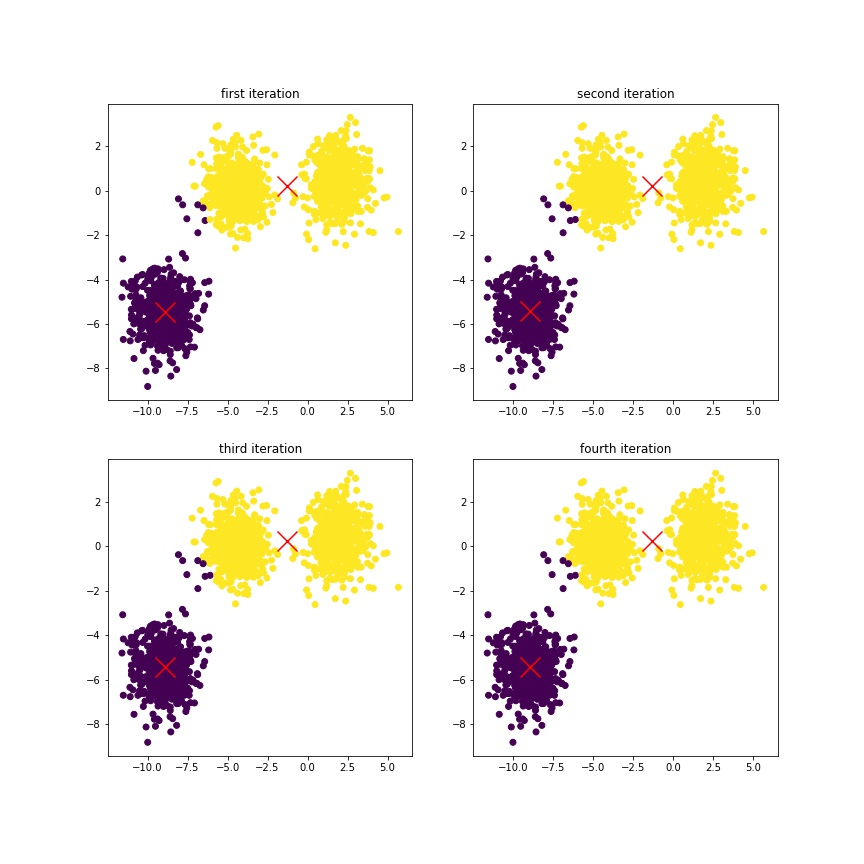
\includegraphics[width=10cm]{EvolKmeans.jpg}  
\vspace*{-6mm}
\end{center}
\caption{Evolution of cluster means and cluster assignments within $k$-means.}
\label{fig:first_iter_kmeans}
\end{figure}

While Algorithm \ref{alg:kmeansimpl} is guaranteed to terminate after a 
finite number of iterations, the delivered cluster assignments and cluster 
means might only be (approximations) of local minima of the clustering error 
\eqref{equ_def_emp_risk_kmeans} (see Figure \ref{fig_emp_risk_k_means}). 

To escape local minima, it is useful to run Algorithm \ref{alg:kmeansimpl} 
several times, using different initializations for the cluster means, 
and picking the cluster assignments $\{ y^{(\sampleidx)} \}_{\sampleidx=1}^{\samplesize}$ 
with smallest clustering error \eqref{equ_def_emp_risk_kmeans}. 

\begin{figure}[htbp]
\begin{center}
%\includegraphics[height=0.2\textheight]{images/ellbow.pdf}
    \begin{tikzpicture}
               \draw[  thick, domain=-1:2.5] plot (2*\x,  {\x^2-3*\x^3+\x+\x^4}) node [right] {$\emperror \big( \{\vm^{(c)}\}_{c=1}^{k},\{y^{(\sampleidx)}\}_{\sampleidx=1}^{\samplesize} \mid \dataset \big)$}; 
               \draw[  thick,fill=blue]  (-1.1,-0.45) circle (0.05cm) node[below] {local minimum}; 
     \end{tikzpicture}
\end{center}
\caption{The clustering error $\emperror \big( \{\vm^{(\clusteridx)}\}_{\clusteridx=1}^{\nrcluster},\{y^{(\sampleidx)}\}_{\sampleidx=1}^{\samplesize} \mid \dataset \big)$ (see \eqref{equ_def_emp_risk_kmeans}), 
which is minimized by $k$-means, is a non-convex function of 
the cluster means and assignments. The $k$-means algorithm 
can get trapped around a local minimum.} \label{fig_emp_risk_k_means}
\end{figure}

Up till now, we have assumed the number $k$ of clusters 
to be given before hand. In some applications it is unclear
what a good choice for $k$ is. The choice for the number 
$k$ of clusters depends on how the clustering methods is 
used within an overall ML application. If the clustering method 
serves as a pre-processing for a supervised ML problem, we 
could try out different values of the number $k$ and determine, 
for each choice $k$, the corresponding validation error. We 
pick then the value of $k$ which results in the smallest validation error. 

Another approach to choosing $k$ is the so-called ``elbow-method''. 
We run the $k$-means Algorithm \ref{alg:kmeansimpl} for different choice 
for $k$. For each choice of $k$, Algorithm \ref{alg:kmeansimpl} delivers a 
different (approximate) optimum empirical error $$\mathcal{E}^{(\nrcluster)} = \emperror \big( \{\vm^{(\clusteridx)}\}_{\clusteridx=1}^{\nrcluster},\{y^{(\sampleidx)}\}_{\sampleidx=1}^{\samplesize} \mid \dataset \big).$$ 
We then plot the minimum empirical error $\mathcal{E}^{(k)}$ as a 
function of the number $k$ of clusters. Figure \ref{fig_ellbow} depicts 
an example for such a plot which typically starts with a steep decrease 
for increasing $k$ and then flattening out for larger values of $k$. 
Finally, the choice of $k$ might be guided by some probabilistic 
model which specifies a prior distribution of the values for $k$. 


\begin{figure}
\begin{center}
%\includegraphics[height=0.2\textheight]{images/ellbow.pdf}
    \begin{tikzpicture}
          \begin{axis}
          [ylabel=$\mathcal{E}^{(k)}$,
              xlabel=$k$]
           %   \addplot[domain=-11:-5.1] {1/(x+5)};
             % \addplot[domain=-4.9:0] {-1/(x+5)};
              \addplot[domain=1:2, ultra thick] {10-x^3};
              \addplot[domain=2:10, ultra thick] {2+1/5-x/10};
         %     \addplot[mark=*,only marks] coordinates {(-3,4)(0,-3)(2,10)};
         %     \addplot[mark=*,fill=white,only marks] coordinates {(-3,-.5)
           %        (0,-.2)(0,2)(2,-2)};
          \end{axis}
     \end{tikzpicture}
\end{center}
\caption{The clustering error $\mathcal{E}^{(k)}$ achieved by $k$-means for increasing number $k$ of clusters.}
\label{fig_ellbow}
\end{figure}




\section{Soft Clustering with Gaussian Mixture Models}
\label{sec_soft_clustering}

The cluster assignments obtained from hard-clustering 
methods, such as Algorithm \ref{alg:kmeansimpl}, provide 
rather coarse-grained information. Indeed, even if two data 
points $\vx^{(\sampleidx)}, \vx^{(j)}$ are assigned to the 
same cluster $\clusteridx$, their distances to the cluster mean $\vm^{(\clusteridx)}$ 
might be very different. For some applications, we would 
like to have a more fine-grained information about the cluster 
assignments. 

%In particular, we are interested in the degree by which a datapoint belongs to a particular cluster. 
Soft-clustering methods provide such fine-grained information 
by explicitly modelling the degree (or confidence) by which 
a particular datapoint belongs to a particular cluster. More 
precisely, soft-clustering methods track for each datapoint 
$\vx^{(\sampleidx)}$ the degree of belonging to each of the 
clusters $\clusteridx \in \{1,\ldots,\nrcluster\}$.  

A principled approach to modelling a degree of belonging to 
different clusters is based on a probabilistic (generative) model 
for the dataset $\dataset = \{ \vx^{(\sampleidx)} \}_{\sampleidx=1}^{\samplesize}$. 
This approach identifies a cluster with a probability distribution. 
One popular choice for this distribution is the multivariate normal 
distribution 
\begin{equation}
\label{equ_def_mvn_distribution}
 \mathcal{N} (\vx ; {\bm \mu}, {\bm \Sigma}) = \frac{1}{\sqrt{{\rm det } \{ 2 \pi  {\bm \Sigma} \} }} \exp\big( - (1/2) (\vx\!-\!{\bm \mu})^{T}  {\bm \Sigma}^{-1} (\vx\!-\!{\bm \mu})  \big)
\end{equation} 
of a Gaussian random vector with mean ${\bm \mu}$ and (invertible) covariance 
matrix ${\bf \Sigma}$.\footnote{Note that the distribution \eqref{equ_def_mvn_distribution} 
is only defined for an invertible (non-singular) covariance matrix ${\bm \Sigma}$.}

Each cluster $\clusteridx \in \{1,\ldots,\nrcluster\}$ is represented by a distribution 
of the form \eqref{equ_def_mvn_distribution} with a cluster-specific mean 
${\bm \mu}^{(\clusteridx)} \in \mathbb{R}^{\featuredim}$ and cluster-specific 
covariance matrix ${\bm \Sigma}^{(\clusteridx)} \in \mathbb{R}^{\featuredim \times \featuredim}$. 

Since we do not know before-hand the cluster assignment $\clusteridx^{(\sampleidx)}$ 
of the datapoint $\vx^{(\sampleidx)}$, we model $\clusteridx^{(\sampleidx)}$ 
as a random variable with probability distribution  
\begin{equation} 
\label{equ_def_cluster_prob}
p_{\clusteridx} \defeq \prob{c^{(\sampleidx)}=\clusteridx} \mbox{ for } \clusteridx=1,\ldots,\nrcluster.
\end{equation}  
The (prior) probabilities $p_{\clusteridx}$, for $\clusteridx=1,\ldots,\nrcluster$, 
are either assumed to be known or estimated from data, e.g., using a maximum 
likelihood method. 

The random cluster assignment $\clusteridx^{(\sampleidx)}$ selects the cluster-specific 
distribution \eqref{equ_def_mvn_distribution} of the random datapoint $\vx^{(\sampleidx)}$, 
\begin{equation}
\label{equ_cond_dist_GMM}
 \prob{\vx^{(\sampleidx)} | \clusteridx^{(\sampleidx)} } = \mathcal{N} (\vx; {\bm \mu}^{(\clusteridx^{(\sampleidx)})}, {\bm \Sigma}^{(\clusteridx^{(\sampleidx)})})
\end{equation} 
with mean vector ${\bm \mu}^{(\clusteridx)}$ and covariance matrix ${\bm \Sigma}^{(\clusteridx)}$. 
%The probability distribution of the random vector depends on the (hidden) cluster index $c^{(\sampleidx)}\in \{1,\ldots,k\}$, 
%such that 
%with some (unknown!) cluster-specific mean vector ${\bm \mu}^{(c)}$ and covariance matrix ${\bm \Sigma}^{(c)}$ associated with cluster $c$. 
%Thus, we consider $\vx^{(\sampleidx)}$ drawn from some cluster, with index $c^{(\sampleidx)} \in \{1,\ldots,k\}$. Each cluster $c \in \{1,\ldots,k\}$ 
%corresponds to a multivariate Gaussian distribution with mean ${\bm \mu}^{(c^)}$ and covariance matrix ${\bm \Sigma}^{(c)}$. 

The modelling of cluster assignments $\clusteridx^{(\sampleidx)}$ as 
(unobserved) random variables suggests a natural definition for degree 
$y^{(\sampleidx)}_{\clusteridx}$ by which datapoint $\vx^{(\sampleidx)}$ 
belongs to cluster $\clusteridx$. We define the degree $y^{(\sampleidx)}_{\clusteridx}$ 
of datapoint $\vx^{(\sampleidx)}$ belonging to cluster $\clusteridx$ as 
the ``a-posteriori'' probability of the cluster assignment $\clusteridx^{(\sampleidx)}$ 
being equal to $\clusteridx \in \{1,\ldots,\nrcluster\}$: 
\begin{equation}
\label{equ_def_deg_belonging_prob}
y^{(\sampleidx)}_{\clusteridx} \defeq \prob{ \clusteridx^{(\sampleidx)} = \clusteridx | \dataset}.
%y^{(\sampleidx)}_{\clusteridx} \defeq \prob{ \clusteridx^{(\sampleidx)}= \clusterfidx | \dataset}
\end{equation} 
By their very definition \eqref{equ_def_deg_belonging_prob}, 
the degrees of belonging $y^{(\sampleidx)}_{\clusteridx}$ always 
sum to one, 
\begin{equation} 
\label{equ_dob_sum_to_one}
\sum_{\clusteridx=1}^{\nrcluster} y^{(\sampleidx)}_{\clusteridx}=1 \mbox{ for each } \sampleidx=1,\ldots,\samplesize.
\end{equation}  

It is important to note that we use the conditional cluster 
probability \eqref{equ_def_deg_belonging_prob}, conditioned 
on the dataset $\dataset$, for defining the degree of belonging $y^{(\sampleidx)}_{\clusteridx}$. 
This is reasonable since the degree of belonging $y^{(\sampleidx)}_{\clusteridx}$ 
depends on the overall (cluster) geometry of the data set $\dataset$.

A probabilistic model for the observed datapoints $\vx^{(\sampleidx)}$ 
is obtained by considering each datapoint $\vx^{(\sampleidx)}$ as a 
random draw from the distribution $\mathcal{N} (\vx ; {\bm \mu}^{(\clusteridx^{(\sampleidx)})}, {\bm \Sigma}^{(\clusteridx^{(\sampleidx)})})$ with some cluster $c^{(\sampleidx)}$. 

Since the cluster indices $\clusteridx^{(\sampleidx)}$ are unknown,\footnote{After all, the goal 
of soft-clustering is to estimate the cluster indices $\clusteridx^{(\sampleidx)}$.} 
we model them as random variables. In particular, we model the cluster indices 
$\clusteridx^{(\sampleidx)}$ as i.i.d.\ with probabilities $p_{\clusteridx} = \prob{ c^{(\sampleidx)} = \clusteridx}.$ 

The overall probabilistic model \eqref{equ_cond_dist_GMM}, \eqref{equ_def_cluster_prob} 
amounts to a {\bf Gaussian mixture model} (GMM). The marginal distribution $\prob{\vx^{(\sampleidx)}}$, 
which is the same for all datapoints $\vx^{(\sampleidx)}$, is a (additive) mixture of 
multivariate normal (Gaussian) distributions, 
\begin{equation} 
\label{equ_def_GMM}
 \prob{\vx^{(\sampleidx)}} = \sum_{\clusteridx=1}^{\nrcluster} \underbrace{\prob{\clusteridx^{(\sampleidx)}=\clusteridx}}_{p_{\clusteridx}}  \underbrace{\prob{\vx^{(\sampleidx)} | \clusteridx^{(\sampleidx)}=\clusteridx}}_{\mathcal{N}(\vx^{(\sampleidx)};{\bm \mu}^{(\clusteridx)}, {\bm \Sigma}^{(\clusteridx)})}. 
\end{equation} 
The cluster assignments $\clusteridx^{(\sampleidx)}$ are hidden (unobserved) random 
variables. We thus have to infer or estimate these variables from the observed 
datapoints $\mathbf{x}^{(\sampleidx)}$ which are i.i.d.\ realizations of the GMM \eqref{equ_def_GMM}. 

\begin{figure}
\begin{center}
\begin{tikzpicture}[scale=0.4]
\draw [thick] \boundellipse{0,0}{10}{5} node[right]  {${\bm \mu^{(1)}}$};
 \fill (0,0) circle (2pt) ; 
  \node [right] at (0,5.5) {$ {\bm \Sigma}^{(1)}$} ; 
\draw [thick] \boundellipse{11,1}{-2}{4} node[right]  {${\bm \mu^{(2)}}$};
 \fill (11,1) circle (2pt) ; 
   \node [right] at (11,5.5) {$ {\bm \Sigma}^{(2)}$} ; 
\draw [thick] \boundellipse{-9,4}{2}{3} node[left,xshift=3mm,yshift=3mm]  {$\,\,{\bm \mu^{(3)}}$}; 
 \fill (-9,4) circle (2pt) ; 
 \node [right] at (-9,8) {$ {\bm \Sigma}^{(3)}$} ; 
\end{tikzpicture}
\end{center}
\label{fig_GMM_elippses}
\caption{The GMM \eqref{equ_def_GMM} yields a probability 
	density function which is a weighted sum of multivariate 
	normal distributions $\mathcal{N}({\bm \mu}^{(\clusteridx)}, {\bm \Sigma}^{(\clusteridx)})$. 
    The weight of the $c$-th component is the cluster probability 
    $ \prob{c^{(\sampleidx)}=\clusteridx}$.}
\end{figure}
%\end{document}

Using the GMM \eqref{equ_def_GMM} for explaining the observed 
datapoints $\vx^{(\sampleidx)}$ turns the clustering problem into 
a {\bf statistical inference} or {\bf parameter estimation problem} \cite{kay,LC}. 
The estimation problem is to estimate the true underlying cluster 
probabilities $p_{\clusteridx}$ (see \eqref{equ_def_cluster_prob}), cluster 
means ${\bm \mu}^{(\clusteridx)}$ and cluster covariance matrices 
${\bm \Sigma}^{(\clusteridx)}$ (see \eqref{equ_cond_dist_GMM}) from 
the observed datapoints $\dataset = \{ \vx^{(\sampleidx)} \}_{\sampleidx=1}^{\samplesize}$. 
The datapoints $\vx^{(\sampleidx)}$ are realizations of i.i.d.\ random vectors with 
the common probability distribution \eqref{equ_def_GMM}. 
%Having estimates for the GMM parameters allows us to compute an estimate (approximation) of the ``a-posteriori'' probability 
%$\prob\{ c^{(\sampleidx)}= c | \dataset \}$, which we consider as the ``true'' degree of datapoint $\vx^{(\sampleidx)}$ belonging to cluster $c$. 

We denote the estimates for the GMM parameters by $\hat{p}_{\clusteridx} (\approx p_{\clusteridx})$, $\vm^{(\clusteridx)} (\approx {\bm \mu}^{(\clusteridx)})$ and 
$\mathbf{C}^{(\clusteridx)} (\approx {\bm \Sigma}^{(\clusteridx)})$, respectively. 
Based on these estimates, we can then compute an estimate $\hat{y}_{\clusteridx}^{(\sampleidx)}$ 
of the (a-posterior) probability 
\begin{equation} 
y_{\clusteridx}^{(\sampleidx)} = \prob{c^{(\sampleidx)} = \clusteridx \mid \dataset }
\end{equation} 
of the $\sampleidx$-th datapoint $\vx^{(\sampleidx)}$ belonging 
to cluster $\clusteridx$, given the observed dataset $\dataset$. 

This estimation problem becomes significantly easier by operating 
in an alternating fashion. In each iteration, we first compute a new 
estimate $\hat{p}_{c}$ of the cluster probabilities $p_{\clusteridx}$, 
given the current estimate $\vm^{(\clusteridx)}, \mathbf{C}^{(\clusteridx)}$ 
for the cluster means and covariance matrices. Then, using this 
new estimate $\hat{p}_{\clusteridx}$ for the cluster probabilities, 
we update the estimates $\vm^{(\clusteridx)}, \mathbf{C}^{(\clusteridx)}$ 
of the cluster means and covariance matrices. Then, using the 
new estimates $\vm^{(\clusteridx)}, \mathbf{C}^{(\clusteridx)}$, we 
compute a new estimate $\hat{p}_{\clusteridx}$ and so on. By repeating 
these two steps, we obtain an iterative soft-clustering method which 
is summarized in Algorithm \ref{alg:softclustering}. 

%Let us, for ease of exposition, restrict to the case of $k\!=\!2$ clusters $\clusteridx\!\in\!\{1,2\}$. The generalization to $k\!>\!2$ clusters is easy. 
%For $k=2$, we only need to track the degree of belonging $y_{1}^{(\sampleidx)}$ to cluster $\clusteridx=1$ since $y_{2}^{(\sampleidx)}\!=\!1\!-\!y_{1}^{(\sampleidx)}$ (see \eqref{equ_dob_sum_to_one}). 
%The estimates of the probabilities can be written as $\hat{p}_{1} = \samplesize_{1}/\samplesize$ and $\hat{p}_{2} = \samplesize_{2}/\samplesize$ 
%with $\samplesize_{1} = \sum_{\sampleidx=1}^{\samplesize} y^{(\sampleidx)}_{1}$ and $\samplesize_{1} = \sum_{\sampleidx=1}^{\samplesize} y^{(\sampleidx)}_{2}$. 
%The quantities $\samplesize_{1}, \samplesize_{2}$ can be interpreted as {\bf effective cluster sizes}. 
\begin{algorithm}[htbp]
\caption{``A Soft-Clustering Algorithm'' \cite{BishopBook}}\label{alg:softclustering}

\begin{algorithmic}[1]
\renewcommand{\algorithmicrequire}{\textbf{Input:}}
\renewcommand{\algorithmicensure}{\textbf{Output:}}
\Require   dataset $\dataset=\{ \vx^{(\sampleidx)}\}_{\sampleidx=1}^{\samplesize}$; number $k$ of clusters. 
\Statex\hspace{-6mm}{\bf Initialize:} use initial guess for GMM parameters $\{\mathbf{m}^{(\clusteridx)},\mathbf{C}^{(\clusteridx)},\hat{p}_{\clusteridx}\}_{\clusteridx=1}^{\nrcluster}$ 
\Repeat
\vspace*{2mm}
\State for each datapoint $\vx^{(\sampleidx)}$ and cluster $\clusteridx \in \{1,\ldots,\nrcluster\}$, update degrees of belonging
\vspace*{-1mm}
\begin{align}
\label{equ_update_soft_cluster_assignm}
y_{c}^{(\sampleidx)} & =  \frac{\hat{p}_{\clusteridx} \mathcal{N}(\vx^{(\sampleidx)};\mathbf{m}^{(\clusteridx)},\mathbf{C}^{(\clusteridx)})}{\sum_{\clusteridx'=1}^{\nrcluster} \hat{p}_{\clusteridx'}\mathcal{N}(\vx^{(\sampleidx)};\mathbf{m}^{(\clusteridx')},\mathbf{C}^{(\clusteridx')})} %\nonumber \\
%y_{2}^{(\sampleidx)} & = 1- y_{1}^{(\sampleidx)} 
\end{align}
\State for each cluster $\clusteridx \in \{1,\ldots,\nrcluster\}$, update estimates of GMM parameters: 
\begin{itemize} 
\item cluster probability $\hat{p}_{\clusteridx}\!=\!\samplesize_{\clusteridx}/\samplesize$, with effective cluster size $\samplesize_{\clusteridx}\!=\!\sum\limits_{\sampleidx=1}^{\samplesize} y_{\clusteridx}^{(\sampleidx)}$
\item cluster mean $\mathbf{m}^{(\clusteridx)} = (1/\samplesize_{\clusteridx}) \sum\limits_{\sampleidx=1}^{\samplesize} y_{\clusteridx}^{(\sampleidx)} \vx^{(\sampleidx)}$ 
\item cluster covariance matrix $\mathbf{C}^{(\clusteridx)}  = (1/\samplesize_{\clusteridx}) {\sum\limits_{\sampleidx=1}^{\samplesize} y_{\clusteridx}^{(\sampleidx)} \big(\vx^{(\sampleidx)}\!-\!\mathbf{m}^{(\clusteridx)}\big)   \big(\vx^{(\sampleidx)}\!-\!\mathbf{m}^{(\clusteridx)}\big)^{T} }$
\end{itemize}
\vspace*{1mm}
\Until convergence \label{equ_conv_soft_clustering_algo}
\Ensure soft cluster assignments $\vy^{(\sampleidx)}=(y_{1}^{(\sampleidx)},\ldots,y_{k}^{(\sampleidx)})^{T}$ for each datapoint $\vx^{(\sampleidx)}$ 
\end{algorithmic}
\end{algorithm}

As for $k$-means, we can interpret the soft clustering problem 
as an instance of the ERM principle discussed in Chapter \ref{ch_Optimization}. 
Indeed, Algorithm \ref{alg:softclustering} aims at minimizing the 
empirical risk 
\begin{equation} 
\label{equ_def_emp_risk_soft_clustering}
\emperror \big( \{ \vm^{(\clusteridx)}, \mathbf{C}^{(\clusteridx)}, \hat{p}_{\clusteridx} \}_{\clusteridx=1}^{\nrcluster} \mid \dataset \big)=
 - \log {\rm Prob} \big\{\dataset; \{ \vm^{(\clusteridx)}, \mathbf{C}^{(\clusteridx)}, \hat{p}_{\clusteridx} \}_{\clusteridx=1}^{\nrcluster}\big\}. 
\end{equation} 

The interpretation of Algorithm \ref{alg:softclustering} as a 
method for minimizing the empirical risk \eqref{equ_def_emp_risk_soft_clustering} 
suggests a stopping criterion. We can monitor the decrease of the empirical risk 
$$ - \log {\rm Prob} \big\{\dataset; \{ \vm^{(\clusteridx)}, \mathbf{C}^{(\clusteridx)}, \hat{p}_{\clusteridx} \}_{\clusteridx=1}^{\nrcluster}\big\}$$
to decide when to stop iterating (see step \ref{equ_conv_soft_clustering_algo} 
of Algorithm \ref{alg:softclustering}). % the termination criterion. % Algorithm \ref{alg:softclustering}. 

Similar to $k$-means Algorithm \ref{alg:kmeans}, also the soft clustering 
Algorithm \ref{alg:softclustering} suffers from the problem of getting stuck 
in local minima of the empirical risk \eqref{equ_def_emp_risk_soft_clustering}. 
As for $k$-means, we can avoid local minima by running Algorithm \ref{alg:softclustering} 
several times, each time with a different initialization for the GMM parameter 
estimates $ \{ \vm^{(c)}, \mathbf{C}^{(c)}, \hat{p}_{c} \}_{c=1}^{k}$ and then 
picking the result which yields the smallest empirical risk \eqref{equ_def_emp_risk_soft_clustering}.  

The empirical risk \eqref{equ_def_emp_risk_soft_clustering} underlying the 
soft-clustering Algorithm \ref{alg:softclustering} is essentially a {\bf log-likelihood function}. 
Thus, Algorithm \ref{alg:softclustering} can be interpreted as an {\bf approximate maximum 
likelihood} estimator for the true underlying GMM parameters $\{{\bm \mu}^{(c)},{\bm \Sigma}^{(c)},p_{c}\}_{c=1}^{k}$. 
In particular, Algorithm \ref{alg:softclustering} is an instance of a generic 
approximate maximum likelihood technique referred to as {\bf expectation maximization} 
(EM) (see \cite[Chap. 8.5]{hastie01statisticallearning} for more details). 
The interpretation of Algorithm \ref{alg:softclustering} as a special case of 
EM allows to characterize the behaviour of Algorithm \ref{alg:softclustering} 
using existing convergence results for EM methods \cite{XuJordan1996}. 
%???? Discuss EM principle in more detail; point out relation to recent work of Arora on Factorization methods such as Dictionary Learning, proving global convergence 
%New Algorithms for Learning Incoherent and Overcomplete Dictionaries, Sanjeev Arora, Rong Ge, Ankur Moitra
%https://arxiv.org/pdf/1510.06096.pdf
%
%Arora, Sanjeev, Rong Ge, Ankur Moitra, and Sushant Sachdeva.
%?Provable ICA with Unknown Gaussian Noise, and Implications
%for Gaussian Mixtures and Autoencoders.? Algorithmica 72, no. 1
%(March 4, 2015): 215?236.
%??????

There is an interesting link between the soft-clustering 
Algorithm \ref{alg:softclustering} and $k$-means. The 
$k$-means algorithm can be interpreted as an extreme 
case of soft-clustering Algorithm \ref{alg:softclustering}. 
Consider fixing the cluster covariance matrices $ {\bm \Sigma}^{(c)}$ 
within the GMM \eqref{equ_cond_dist_GMM} to be the scaled identity: 
\begin{equation}
\label{equ_def_special_case}
 {\bm \Sigma}^{(c)}= \sigma^{2} \mathbf{I} \mbox{ for all } c \in \{1,\ldots,k\}.  
\end{equation} 
We assume the covariance matrix \eqref{equ_def_special_case}, 
with a particular value for $\sigma^{2}$, to be the actual ``correct'' 
covariance matrix for cluster $c$. %The estimates $\mathbf{C}^{(c)}$ 
%for the covariance matrices are then trivially given by $\mathbf{C}^{(c)} =  {\bm \Sigma}^{(c)}$.  
Thus, we replace the covariance matrix updates in Algorithm \ref{alg:softclustering} 
with $\mathbf{C}^{(c)} \defeq  {\bm \Sigma}^{(c)}$.
 
When choosing a very small variance $\sigma^{2}$ in \eqref{equ_def_special_case}, 
the update \eqref{equ_update_soft_cluster_assignm} tends to enforce 
$y_{\clusteridx}^{(\sampleidx)} \in \{0,1\}$. Thus, each datapoint $\vx^{(\sampleidx)}$ 
is associated exclusively to the cluster $\clusteridx$ whose cluster mean $\vm^{(\clusteridx)}$ 
has minimum Euclidean distance to the datapoint $\vx^{(\sampleidx)}$. 
To summarize, for $\sigma^{2} \rightarrow 0$, the soft-clustering update 
\eqref{equ_update_soft_cluster_assignm} reduces to the hard cluster 
assignment update \eqref{equ_cluster_assign_update} of the $k$-means Algorithm \ref{alg:kmeans}. 

\section{Density Based Clustering with DBSCAN}

Both k-means and GMM cluster datapoints using the Euclidean distance, 
which is a natural measure of similarity in many cases. However, in some 
applications, the data conforms to a different non-Euclidean structure. 
One example for a non-Euclidean structure is a graph or network structure. 
Here, two datapoints are considered similar if they can be reached by 
intermediate datapoints that have a small Euclidean distance. Thus, 
two datapoints can be similar in terms of connectivity, even if their 
Euclidean distance is large.Density-based spatial clustering of 
applications with noise (DBSCAN) is a hard clustering method that 
uses a connectivity-based similarity measure. In contrast to k-means 
and the GMM, DBSCAN does not require the number of clusters to 
be pre-defined -  the number will depend on its parameters. Moreover, 
DBSCAN detects outliers that are interpreted as degenerated clusters 
consisting of a single datapoint. For a detailed discussion of how 
DBSCAN works, we refer to https://en.wikipedia.org/wiki/DBSCAN.  DBSCAN 
%is implemented in the DBSCAN class in scikit-learn Documentation 
%can be found here. DBSCAN requires specifying two parameters 
% eps and min_samples. The meaning of these parameter are well explained here. 
%The DBSCAN implementation fit_predict(self, X[, y, sample_weight]) returns cluster labels.

\section{Exercises} 
\subsection{Image Compression with k-means} 
use k-means to compress a RGB bitmap image. Instead of RGB values 
we need to store only cluster index and the cluster means. 

\subsection{Compression with k-means} 
Consider $\samplesize=10000$ datapoints are characterized by two 
floating point numbers (32 bit). We apply k-means to cluster the 
data set into two clusters. How many bits do we need to store the 
clustering ? 


\newpage
\chapter{Feature Learning} 
\label{ch_FeatureLearning}

\begin{quote}
``Solving Problems By Changing the Viewpoint.''
\end{quote}

\begin{figure}[htbp]
\begin{center}
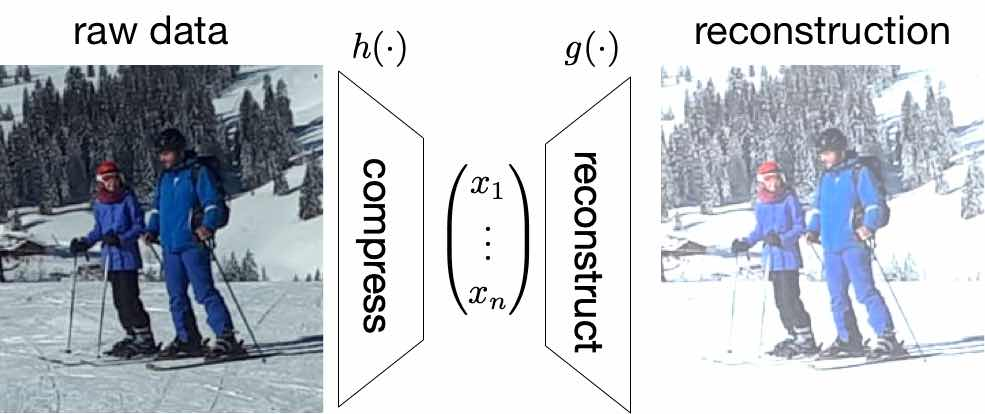
\includegraphics[width=0.7\textwidth]{DimRed.jpg}  
\end{center}
\caption{Dimensionality reduction methods aim at finding a map $h$ which maximally 
	compresses the raw data while still allowing to accurately reconstruct the original 
	datapoint from a small number of features $x_{1},\ldots,x_{\featuredim}$.}
\label{fig_dimred}
\end{figure}

%????? Discuss relation to Information Bottleneck and universal source coding ??????

%????? Discuss a simple method for dim. red. for binary data ????

Chapter \ref{ch_Elements_ML} discussed features as those properties of a datapoint that can 
be measured or computed easily. Sometimes the choice of features follows 
naturally from the available hard and software. As an example we might use 
the measurements delivered by sensing devices as features. Beside direct 
sensor readings, we might construct new features by simple computations. 

Consider datapoints representing ski days which are characterized by the 
minimum daytime temperature as their feature $x$. Then we might construct 
new features of a datapoint by computing  powers $x^{2}$ and $x^{3}$. 
Another feature is obtained by $x+5$. Each of these computations produces 
a new feature. Which of these additional features are most useful?
%Feature learning methods aim at learning how to compute most relevant features 
%given the raw datapoint. One example 
%
%Roughly speaking, ML methods exploit the intrinsic geometry of (large) sets of 
%datapoints to compute predictions. By definition, we represent these datapoints 
%as elements of the feature space $\featurespace$. Note that the features are 
%a design choice so we can shape the intrinsic geometry of the datapoints by 
%using different choices for the features (and feature space). 

Feature learning methods automate the choice of finding a good features. These 
methods learn a map that read in the original raw features and transform them to 
a set of new features. A subclass of feature learning methods are dimensionality 
reduction methods, where the new feature space has a (much) smaller dimension 
than the original feature space (see Section \ref{sec_dim_red}). Sometimes 
it might be useful to change to a higher-dimensional feature space. Section \ref{sec_dim_increas} 
discusses feature learning method that result in new feature vectors which 
are longer than the raw feature vector 


??? Develop feature learning as an approximation problem. The raw data 
is the vector to be approximated. The approximation has to be in a (small) 
subspace which is spanned by all possible low-dimensional feature vectors???

%Supervised ML methods often 
%rely on the principle that near-by datapoints should have similar label values. 
%There is a great deal of ways to define this notion of ``near-by''.  
\section{Dimensionality Reduction} 
\label{sec_dim_red}

Consider a ML method that aims at predicting the label $y$ of a datapoint $\vz$ 
based on some features $\vx$ which characterize the datapoint $\vz$. Intuitively, it 
should be beneficial to use as many features as possible. Indeed, the more features 
of a datapoint we know, the more we should know about its label $y$. 
%since having more information 
%about a datapoint can only help us in the task of predicting the label $y$. 

There are, however, two pitfalls in using an unnecessarily large number of features. 
The first one is a {\bf computational pitfall} and the second one is a {\bf statistical pitfall}. 
The larger the feature vector $\vx \in \mathbb{R}^{\featuredim}$ (with large $\featuredim$), 
the more computation (and storage) is required for executing the resulting ML method. 
Moreover, using a large number of features makes the resulting ML methods more prone to 
overfitting. Indeed, linear regression will overfit when using feature vectors $\vx\!\in\!\mathbb{R}^{\featuredim}$ 
whose length $\featuredim$ exceeds the number $\samplesize$ of labeled datapoints used 
for training (see Chapter \ref{ch_overfitting_regularization}). 

Thus, both from a computational and statistical perspective, it is beneficial to use 
only the maximum necessary amount of relevant features. A key challenge here is 
to select those features which carry most of the relevant information required for 
the prediction of the label $y$. Beside coping with overfitting and limited computational 
resources, dimensionality reduction can also be useful for data visualization. Indeed, if 
the resulting feature vector has length $d=2$, we can use scatter plots to depict datasets. 

The basic idea behind most dimensionality reduction methods is quite simple. As 
illustrated in Figure \ref{fig_dimred}, these methods aim at learning (finding) a ``compression'' 
map that transforms a raw datapoint $\vz$ to a (short) feature vector $\vx=(x_{1},\ldots,x_{\featuredim})^{T}$ 
in such a way that it is possible to find (learn) a ``reconstruction'' map which allows to accurately 
reconstruct the original datapoint from the features $\vx$. The compression and reconstruction 
map is typically constrained to belong some set of computationally feasible maps or hypothesis 
space (see Chapter \ref{ch_some_examples} for different examples of hypothesis spaces). In what 
follows we restrict ourselves to using only linear maps for compression and reconstruction leading 
to principal component analysis. The extension to non-linear maps using deep neural networks 
is known as {\bf deep autoencoders} \cite[Ch. 14]{Goodfellow-et-al-2016}. 


\section{Principal Component Analysis} 
\label{sec_pca}

%We will now discuss some basic but powerful methods for efficiently constructing relevant features $\vx$ for a datapoint $\vz$. 
Consider a datapoint $\vz \in \mathbb{R}^{D}$ which is represented by a (typically very long) 
vector of length $D$. The length $D$ of the raw feature vector might be easily of the order of 
millions. To obtain a small set of relevant features $\vx \in \mathbb{R}^{\featuredim}$, we apply 
a linear transformation to the datapoint: 
\begin{equation} 
\label{equ_feat_learning_matrix}
\vx = \mathbf{W} \vz.
\end{equation}
Here, the ``compression'' matrix $\mathbf{W} \in \mathbb{R}^{\featuredim \times D}$ maps 
(in a linear fashion) the large vector $\vz \in \mathbb{R}^{D}$ to a smaller feature vector $\vx \in \mathbb{R}^{\featuredim}$. %In what follows, we consider particular choice for the matrix $\mathbf{W}$. 


It is reasonable to choose the compression matrix $\mathbf{W} \in \mathbb{R}^{\featuredim \times D}$ 
in \eqref{equ_feat_learning_matrix} such that the resulting features $\vx \in \mathbb{R}^{\featuredim}$ 
allow to approximate the original datapoint $\vz \in \mathbb{R}^{D}$ as accurate as possible. We can 
approximate (or recover) the datapoint $\vz \in \mathbb{R}^{D}$ back from the features $\vx$ by 
applying a reconstruction operator $\mathbf{R} \in \mathbb{R}^{D \times \featuredim}$, which is 
chosen such that 
\begin{equation} 
\label{equ_approx_linear_PCA}
\vz \approx \mathbf{R} \vx \stackrel{\eqref{equ_feat_learning_matrix}}{=} \mathbf{R} \mathbf{W} \vz. 
\end{equation} 

The approximation error $\emperror \big( \mathbf{W},\mathbf{R} \mid \dataset\big)$ resulting 
when \eqref{equ_approx_linear_PCA} is applied to each datapoint in a 
dataset $\dataset=  \{ \vz^{(\sampleidx)}\}_{\sampleidx=1}^{\samplesize}$ is then
\begin{equation} 
\label{equ_app_error_PCA}
\emperror \big( \mathbf{W},\mathbf{R} \mid \dataset\big) = (1/\samplesize) \sum_{\sampleidx=1}^{\samplesize} \| \vz^{(\sampleidx)} - \mathbf{R} \mathbf{W} \vz^{(\sampleidx)} \|. 
\end{equation} 

One can verify that the approximation error $\emperror \big( \mathbf{W},\mathbf{R} \mid \dataset\big)$ 
can only by minimal if the compression matrix $\mathbf{W}$ is of the form
\begin{equation}
\label{equ_def_PCA_W}
\mathbf{W} = \mathbf{W}_{\rm PCA} \defeq \big( \mathbf{u}^{(1)},\ldots, \mathbf{u}^{(\featuredim)} \big)^{T} \in \mathbb{R}^{\featuredim \times D}, 
\end{equation} 
with $\featuredim$ orthonormal vectors $\mathbf{u}^{(l)}$ which correspond to the 
$\featuredim$ largest eigenvalues of the {\bf sample covariance matrix} 
\begin{equation} 
\label{equ_def_Q_PCA}
\mathbf{Q} \defeq (1/\samplesize) \mathbf{Z}^{T} \mathbf{Z} \in \mathbb{R}^{D \times D} 
\end{equation}
with data matrix $\mathbf{Z}\!=\!\big( \vz^{(1)}, \ldots, \vz^{(\samplesize)} \big)^{T}\!\in\!\mathbb{R}^{\samplesize \times D}$.
\footnote{Some authors define the data matrix as $\mZ\!=\!\big( \widetilde{\vz}^{(1)}, \ldots, \widetilde{\vz}^{(\samplesize)} \big)^{T}\!\in\!\mathbb{R}^{\samplesize \times D}$  using ``centered'' datapoints $\widetilde{\vz}^{(\sampleidx)} - \widehat{\vm}$ 
	obtained by subtracting the average $\widehat{\vm} = (1/\samplesize) \sum_{\sampleidx=1}^{\samplesize} \vz^{(\sampleidx)}$.}
By its very definition \eqref{equ_def_Q_PCA}, the matrix $\mathbf{Q}$ is positive semi-definite so that it allows 
for an eigenvalue decomposition (EVD) of the form \cite{Strang2007}
\vspace*{-2mm}
\begin{equation}
\label{equ_EVD_Q_PCA}
 \mQ=\big(\eigvecCov^{(1)},\ldots,\eigvecCov^{(D)}\big)  \begin{pmatrix}\lambda^{(1)} &  \ldots & 0 \\ 0 & \ddots & 0  \\ 0 & \ldots & \lambda^{(D)} 
 \end{pmatrix} \big(\eigvecCov^{(1)},\ldots,\eigvecCov^{(D)}\big)^{T} \nonumber
\end{equation} 
with real-valued eigenvalues $\lambda^{(1)} \geq \lambda^{(2)}\geq \ldots \geq \lambda^{(D)} \geq 0$ and orthonormal 
eigenvectors $\{ \eigvecCov_{r} \}_{r=1}^{D}$. 

The features $\vx^{(\sampleidx)}$, obtained by applying the compression matrix $\mathbf{W}_{\rm PCA}$ 
\eqref{equ_def_PCA_W} to the raw datapoints $\vz^{(\sampleidx)}$, are referred to as {\bf principal components (PC)}. 
The overall procedure of determining the compression matrix \eqref{equ_def_PCA_W} and, in turn, computing 
the PC vectors $\vx^{(\sampleidx)}$ is known as {\bf principal component analysis (PCA)} and summarized 
in Algorithm \ref{alg_PCA}. 
\begin{algorithm}[htbp]
\caption{Principal Component Analysis (PCA)}\label{alg_PCA}
\begin{algorithmic}[1]
\renewcommand{\algorithmicrequire}{\textbf{Input:}}
\renewcommand{\algorithmicensure}{\textbf{Output:}}
\Require  dataset  $\dataset=\{ \vz^{(\sampleidx)} \in \mathbb{R}^{D} \}_{\sampleidx=1}^{\samplesize}$; number $\featuredim$ of PCs. 
%\Statex\hspace{-6mm}{\bf Initialize:} choose initial cluster means $\vm_{c}$ for $c=1,\ldots,k$.    
%\Repeat
%\State for all $i\!=\!1,\ldots,\samplesize$, do 
\State compute EVD \eqref{equ_EVD_Q_PCA} to obtain orthonormal eigenvectors $\big(\eigvecCov^{(1)},\ldots,\eigvecCov^{(D)}\big)$ 
corresponding to (decreasingly ordered) eigenvalues $\lambda^{(1)} \geq \lambda^{(2)}\geq \ldots \geq \lambda^{(D)} \geq 0$
\vspace*{2mm}
\State construct compression matrix $\mW_{\rm PCA}  \defeq \big( \mathbf{u}^{(1)},\ldots, \mathbf{u}^{(\featuredim)} \big)^{T} \in \mathbb{R}^{\featuredim \times D}$ %  $\vx^{(\sampleidx)} = \mW_{\rm PCA} \vz^{(\sampleidx)}$ with compression matrix \eqref{equ_def_PCA_W}
\vspace*{2mm}
\State compute feature vector $\vx^{(\sampleidx)} = \mW_{\rm PCA} \vz^{(\sampleidx)}$ whose entries are PC of $\vz^{(\sampleidx)}$ %with compression matrix \eqref{equ_def_PCA_W}
%\Until convergence 
\vspace*{2mm}
\State compute approximation error $\emperror^{(\rm PCA)} = \sum_{r = \featuredim+1}^{D} \lambda^{(r)}$ (see \eqref{equ_approx_error_PCA}). 
\vspace*{2mm}
\Ensure $\vx^{(\sampleidx)}$, for $\sampleidx=1,\ldots,\samplesize$, and the approximation error $\emperror^{(\rm PCA)}$. 
\end{algorithmic}
\end{algorithm}
Note that the length $n$ of the feature vectors $\vx$, which is also the number of PCs used, is an 
input parameter of Algorithm \ref{alg_PCA}. The number $n$ can be chosen between $n=0$ and $n=D$. 
However, it can be shown that PCA for $n>m$ is not well-defined. In particular, the orthonormal eigenvectors 
$ \mathbf{u}^{(\featuredim+1)},\ldots, \mathbf{u}^{(D)}$ are not unique. 


From a computational perspective, Algorithm \ref{alg_PCA} essentially amounts to performing an EVD of the sample covariance 
matrix $\mathbf{Q}$ (see \eqref{equ_def_Q_PCA}). Indeed, the EVD of $\mQ$ provides not only the optimal compression matrix 
$\mathbf{W}_{\rm PCA}$ but also the measure $\emperror^{(\rm PCA)}$ for the information loss incurred by replacing the original 
datapoints $\vz^{(\sampleidx)} \in \mathbb{R}^{D}$ with the smaller feature vector $\vx^{(\sampleidx)} \in \mathbb{R}^{\featuredim}$. 
In particular, this information loss is measured by the approximation error (obtained for the optimal reconstruction matrix 
$\mathbf{R}_{\rm opt} = \mathbf{W}_{\rm PCA}^{T}$)
%$\emperror \big( \mathbf{W}_{\rm PCA},\mathbf{R}\mid \dataset\big)$ \eqref{equ_app_error_PCA}) which is given as 
\begin{equation} 
\label{equ_approx_error_PCA}
\emperror^{(\rm PCA)} \defeq \emperror \big( \mathbf{W}_{\rm PCA},\underbrace{\mathbf{R}_{\rm opt}}_{=\mathbf{W}_{\rm PCA}^{T}}\mid \dataset\big) = \sum_{r = \featuredim+1}^{D} \lambda^{(r)}. 
\end{equation} 
As depicted in Figure \ref{fig_ellbow_PCA}, the approximation error  $\emperror^{(\rm PCA)}$ decreases with increasing 
number $\featuredim$ of PCs used for the new features \eqref{equ_feat_learning_matrix}. The maximum error 
$\emperror^{(\rm PCA)} = (1/\samplesize) \sum_{\sampleidx=1}^{\samplesize} \| \vz^{(\sampleidx)} \|^{2}$ is obtained for 
$\featuredim\!=\!0$, which amounts to completely ignoring the datapoints $\vz^{(\sampleidx)}$. In the other extreme case 
where $\featuredim\!=\!D$ and $\vx^{(\sampleidx)}\!=\!\vz^{(\sampleidx)}$, which amounts to no compression at all, the 
approximation error is zero $\emperror^{(\rm PCA)}\!=\!0$. 

\begin{figure}[htbp]
\begin{center}
%\includegraphics[height=0.2\textheight]{images/ellbow.pdf}
    \begin{tikzpicture}
          \begin{axis}
          [ylabel=$\emperror^{(\rm PCA)}$,
              xlabel=$\featuredim$]
           %   \addplot[domain=-11:-5.1] {1/(x+5)};
             % \addplot[domain=-4.9:0] {-1/(x+5)};
              \addplot[domain=1:2, ultra thick] {10-x^3};
              \addplot[domain=2:10, ultra thick] {2+1/5-x/10};
         %     \addplot[mark=*,only marks] coordinates {(-3,4)(0,-3)(2,10)};
         %     \addplot[mark=*,fill=white,only marks] coordinates {(-3,-.5)
           %        (0,-.2)(0,2)(2,-2)};
          \end{axis}
     \end{tikzpicture}
\end{center}
\caption{Reconstruction error $\emperror^{(\rm PCA)}$ (see \eqref{equ_approx_error_PCA}) of PCA for varying number $\featuredim$ of PCs.}
\label{fig_ellbow_PCA}
\end{figure}

\subsection{Combining PCA with Linear Regression} 

One important use case of PCA is as a pre-processing step within an overall ML problem 
such as linear regression (see Section \ref{sec_lin_regression}). As discussed in Chapter 
\ref{ch_overfitting_regularization}, linear regression methods are prone to overfitting 
whenever the datapoints are characterized by feature vectors whose length $D$ exceeds 
the number $\samplesize$ of labeled datapoints used for training. One simple but powerful 
strategy to avoid overfitting is to preprocess the original feature vectors (they are considered 
as the raw datapoints $\vz^{(\sampleidx)}\in \mathbb{R}^{D}$) by applying PCA in order to obtain 
smaller feature vectors $\vx^{(\sampleidx)} \in \mathbb{R}^{\featuredim}$ with $\featuredim < \samplesize$. 

%We will discuss how using PCA avoids overfitting for settings where the raw datapoints $\vz^{(\sampleidx)}$ are high-dimensional, i.e., 
%$\vz^{(\sampleidx)} \in \mathbb{R}^{D}$ with $D$ very large. %????DISCUSS REGRESSION PROBLEM USING WEBCAM SNAPSHOTS?????


\subsection{How To Choose Number of PC?} 
There are several aspects which can guide the choice for the number $\featuredim$ of PCs to be used as features. 
\begin{itemize}
\item for data visualization: use either $\featuredim=2$ or $\featuredim=3$ 
\item computational budget: choose $\featuredim$ sufficiently small such 
that the computational complexity of the overall ML method does not exceed 
the available computational resources.  
\item statistical budget: consider using PCA as a pre-processing step within a linear 
regression problem (see Section \ref{sec_lin_regression}). Thus, we use the output 
$\vx^{(\sampleidx)}$ of PCA as the feature vectors in linear regression. In order to avoid 
overfitting, we should choose $\featuredim < \samplesize$ (see Chapter \ref{ch_overfitting_regularization}). 
\item elbow method: choose $\featuredim$ large enough such that approximation 
error $\emperror^{(\rm PCA)}$ is reasonably small (see Figure \ref{fig_ellbow_PCA}). 
\end{itemize} 



\subsection{Data Visualisation}

If we use PCA with $\featuredim=2$ PC, we obtain feature vectors 
$\vx^{(\sampleidx)} = \mathbf{W} \vz^{(\sampleidx)}$ (see \eqref{equ_feat_learning_matrix}) 
which can be depicted as points in a scatter plot (see Section \ref{equ_subsection_scatterplot}). 
As an example, consider datapoints $\vz^{(\sampleidx)}$ obtained 
from historic recordings of Bitcoin statistics. Each datapoint $\vz^{(\sampleidx)} \in \mathbb{R}^{6}$ 
is a vector of length $D=6$. It is difficult to visualise points in 
an Euclidean space $\mathbb{R}^{D}$ of dimension $D > 2$. We 
apply PCA with $\featuredim=2$ which results in 
feature vectors $\vx^{(\sampleidx)} \in \mathbb{R}^{2}$. Such feature 
vectors can be depicted conveniently as a scatter plot (see Figure \ref{fig_scatterplot_visualization}). 

\begin{figure}[htbp]
\begin{center}
\begin{tikzpicture}
    \begin{axis}[
            axis x line=middle,
            axis y line=middle,
            xmax=5000,
            enlarge y limits=true,
            enlarge x limits=true,
            width=10cm, height=8cm,    
            grid = major,
            grid style={dashed, gray!30},
            ylabel=first PC $x_{1}$,
            xlabel=second PC $x_{2}$,
         ]        
          \addplot[only marks,mark=+] table [x=pc1, y=pc2, col sep = comma] {twopc.csv};
    \end{axis}
\end{tikzpicture}
\end{center}
\caption{A scatter plot of feature vectors $\vx^{(\sampleidx)} = \big(x_{1}^{(\sampleidx)},x_{2}^{(\sampleidx)}\big)^{T}$ 
	whose entries are the first two PCs of the Bitcoin statistics $\vz^{(\sampleidx)}$ of the $\sampleidx$-th day.} 
\label{fig_scatterplot_visualization}
\end{figure}



\subsection{Extensions of PCA}
There have been proposed several extensions of the basic PCA method: 
\begin{itemize}
 \item {\bf kernel PCA \cite[Ch.14.5.4]{hastie01statisticallearning}:} combines PCA with a non-linear feature map (see Section \ref{sec_kernel_methods}). % {\bf non-linear} subspaces by combining PCA with feature map obtained from a kernel function. 
 \vspace*{2mm}
 \item {\bf robust PCA \cite{RobustPCA}:} modifies PCA to better cope with {\bf outliers} in the dataset.
 \vspace*{2mm}
 \item {\bf sparse PCA \cite[Ch.14.5.5]{hastie01statisticallearning}:} requires each PC to depend only on a small number of data attributes $z_{j}$. 
 \vspace*{2mm}
 \item {\bf probabilistic PCA \cite{Roweis98emalgorithms,probabilistic-principal-component-analysis}:} generalizes PCA by using a  {\bf probabilistic (generative) model} for the data. 
\end{itemize}

\section{Linear Discriminant Analysis}

Dimensionality reduction is typically used as a preprocessing step within some overall ML problem such as 
regression or classification. It can then be useful to exploit the availability of labeled data for the design 
of the compression matrix $\mW$ in \eqref{equ_feat_learning_matrix}. However, plain PCA (see Algorithm 
\ref{alg_PCA}) does not make use of any label information provided additionally for the raw datapoints 
$\vz^{(\sampleidx)} \in \mathbb{R}^{D}$. Therefore, the compression matrix $\mW_{\rm PCA}$ delivered 
by PCA can be highly suboptimal as a pre-processing step for labeled datapoints. A principled approach 
for choosing the compression matrix $\mW$ such that datapoints with different labels are well separated 
is {\bf linear discriminant analysis} \cite{hastie01statisticallearning}. 

\section{Random Projections} 
Note that PCA amounts to computing an EVD of the sample covariance matrix 
$\mathbf{Q} = (1/\samplesize) \mathbf{Z} \mathbf{Z}^{T}$ with the data matrix 
$\mathbf{Z} = \big(\vz^{(1)},\ldots,\vz^{(\samplesize)}\big)^{T}$ containing the 
datapoints $\vz^{(\sampleidx)} \in \mathbb{R}^{D}$ as its columns. The computational 
complexity (amount of multiplications and additions) for computing this PCA is lower 
bounded by $\min\{ D^{2}, \samplesize^{2} \}$ \cite{Du08low-complexityprincipal,Sharma2007}. 
This computational complexity can be prohibitive for ML applications with $\featuredim$ 
and $\samplesize$ being of the order of millions (which is already the case if the features 
are pixel values of a $512 \times 512$ RGB bitmap, see Section \ref{sec_feature_space}). 
There is a surprisingly cheap alternative to PCA for finding a good choice for the 
compression matrix $\mathbf{W}$ in \eqref{equ_feat_learning_matrix}. Indeed, a randomly 
chosen matrix $\mathbf{W}$ with entries drawn i.i.d.\ from a suitable probability distribution 
(such as Bernoulli or Gaussian) yields a good compression matrix $\mW$ (see \eqref{equ_feat_learning_matrix}) 
with high probability \cite{Bingham01randomprojection,jung-specesttit}. 

%???? mention LightOn technology https://arxiv.org/abs/1510.06664?????

\section{Information Bottleneck}
We can use information bottleneck for feature learning. Using Gaussian process model, we even 
get closed-form solutions of Gaussian Information Bottleneck. 


\section{Dimensionality Increase} 
\label{sec_dim_increas} 

? Discuss kernel methods; and polynomial regression as special case???

Feature learning methods are mainly dimensionality reduction methods.
However, it might be beneficial to also consider feature learning methods 
that produce new feature vectors which are longer than the raw feature 
vectors. An extreme example for such a feature map are kernel 
methods which map finite length vector to infinite dimensional spaces. 

Mapping raw feature vectors into higher-dimensional spaces might be useful 
if the intrinsic geometry of the datapoints is simpler when looked at in the 
higher-dimensional space. Consider a binary classification problem where 
datapoints are highly inter-winded in the original feature space. By mapping 
into higher-dimensional feature space we might "even-out" this non-linear 
geometry such that we can use linear classifiers in the higher-dimensional space. 

%??? add section on kernel methods which take the other direction, i.e., create longer feature vectors than 
%original raw feature vectors ???

\chapter{Privacy-Preserving ML}
\label{chap_privacy_preserving_ML}

Many ML applications involve datapoints representing individual humans. 
These datapoints might include sensitive data, such as medical records, 
which is subject to privacy protection. This chapter discusses some techniques 
for preprocessing the raw data to protect privacy of individuals while still allowing 
to solve the overall ML task. We will illustrate these techniques using a stylized 
healthcare application. 

\begin{figure}[htbp]
	\centering
	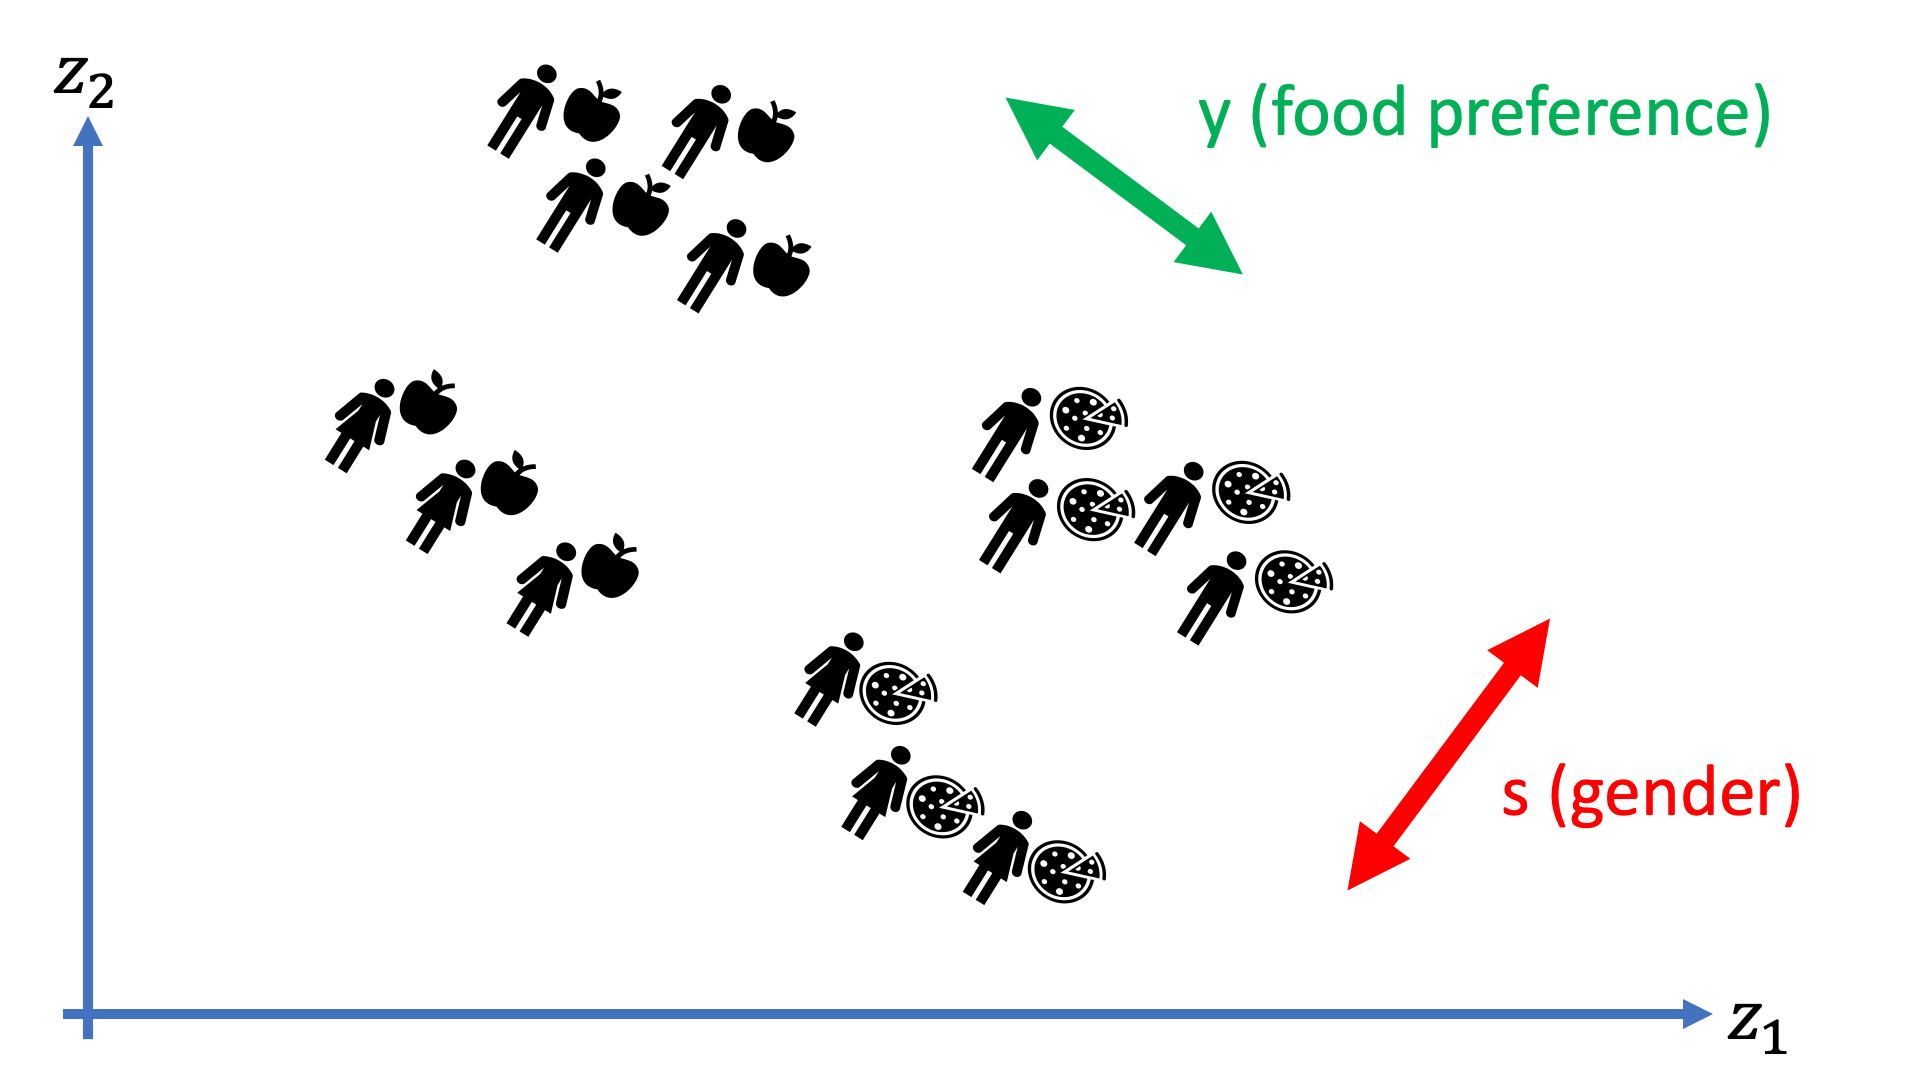
\includegraphics[width=8cm]{PrivacyPreservingCartoon.png}
	\caption{datapoints represent humans. We are interested in the fruit 
		preference of humans. Their gender is considered sensitive information 
		and should not be revealed to ML methods.}
	\label{fig:ppmlcartoon}
\end{figure}

A key challenge for health-care are pandemics. To optimally manage pandemics 
it is important to have accurate information about the dynamics. We can model 
this as a ML problem with datapoints representing humans. One key feature of 
datapoints is if it represents an infected human or not. This data is sensitive 
and typically only available to public health-care institutes. 

Consider the patient database of a hospital which should provide information 
about the average number of infected patients. Instead of directly forward 
the patient files, the hospital must only forward the fraction of infected patients. 
This is an example of privacy-preserving data processing. For a sufficiently large 
number of patients at the hospital (say, more than $1000$), we cannot infer much 
about individual patients just form the fraction of infected patients treated in that 
hospital. 

\section{Privacy-Preserving Feature Learning (Operating on level of individual datapoints)}

Privacy-preserving ML can be implemented using modification of feature learning 
methods discussed in Chapter \ref{ch_FeatureLearning}. Generic feature learning 
methods aim at learning a compressed representation of the raw datapoints which 
contain as much information as possible about the quantity of interest. In contrast, 
privacy-preserving ML does not aim at compression but rather obscuring the raw 
data such that it does not reveal sensible information about datapoints. 


\subsection{Privacy-Preserving Information Bottleneck} %?? info bottleneck with privacy constraints??? 


\subsection{Privacy-Preserving Feature Selection} 
?? ignore features which are sensitive (name, social ID) 
but not very relevant for actual task (e.g. predicting income).    ???

\subsection{Privacy-Preserving Random Projections} 
?? cheap form: random projections/compressed sensing. 
random projections blur features of individual datapoints 
but still allow to learn a sparse linear model using e.g. Lasso ???


\section{Exercises} 
\subsection{Where are you?} 
\label{ex_where_are_you} 
Consider a ML method that uses FMI data for temperature forecasts. 
The ML methods downloads the following sequence of daily temperatures: ??,???,???,??. 
What is the most likely  nearest observation station to the ML user ? 



\section{Federated Learning (Operates on level of local datasets)}
FL method only exchange model parameter updates; no raw local data is revealed; 

 
\chapter{Explainable ML}
\label{chap_explainable_ML}

A key challenge for the successful deployment of ML methods to 
many (critical) application domain is their explainability. Human users 
of ML seem to have a strong desire to get explanations that resolve 
the uncertainty about predictions and decisions obtained from ML 
methods. Explainable ML enables the user to better predict the 
outcomes of ML methods. 

Explainable ML is challenging since explanations must be tailored 
(personalized) to individual users with varying backgrounds. Some 
users might have received university-level education in ML, while 
other users might have no formal training in linear algebra. Linear 
regression with few features might be perfectly interpretable for 
the first group but might be considered a black-box by the latter. 


?????? 
discuss relation between finding good explanations and active 
learning. Active learning aims at finding datapoints (by their features) 
which provide most information about the true model parameters. 
XML aims at finding explanations (e.g. datapoints from training set) 
which provide most information about the prediction provided by 
some black-box ML method. 
?????????????
discuss relation between XML and feature learning. XML can be 
obtained from feature learning methods by learning those subset 
of features which provide most information about the prediction 
(not about the label itself)
?????????????? 


\section{A Model Agnostic Method}
\label{sec_model_agn_xml}

We propose a simple probabilistic model for the predictions and 
user knowledge. This model allows to study explainable ML using 
information theory. Explaining is here considered as the task of 
reducing the ``surprise'' incurred by a prediction. We quantify 
the effect of an explanation by the conditional mutual information 
between the explanation and prediction, given the user background. 

\section{Explainable Empirical Risk Minimization} 
The approach discussed in Section \ref{sec_model_agn_xml} constructs explanations 
for any given ML method such that the user is able to better predict 
the outcome of this ML method. Instead of providing an explanation 
we could also try to make the ML method itself more predictable for 
a user. 


\chapter{Lists of Symbols}

\section{Sets} 
\begin{align} 
&\mathbb{R}  &\quad &\mbox{The set of real numbers $x$.} \nonumber \\
&\mathbb{R}_{+}  &\quad &\mbox{The set of non-negative real numbers $x\geq0$.} \nonumber \\ \nonumber
\end{align} 

\section{Matrices and Vectors} 
\begin{align} 
&\mathbf{I}  &\quad &\mbox{The identity matrix having ones on the main diagonal and zeros off diagonal.} \nonumber \\
&\mathbf{R}^{n}  &\quad &\mbox{The set of all vectors constituted by $n$ real-valued entries.} \nonumber \\
&\mathbf{x}=\big(x_{1},\ldots,x_{n})^{T}  &\quad &\mbox{Some vector of length $n$. The $j$th entry of the vector is denoted $x_{j}$.} \nonumber \\
&\| \mathbf{x}\|_{2}  &\quad &\mbox{The Euclidean norm of the vector $\mathbf{x}$, } \| \mathbf{x}\|_{2} \defeq \sqrt{\sum_{j=1}^{n} x_{j}^{2}}  \nonumber \\
&\| \mathbf{x}\|  &\quad &\mbox{Some norm of the vector $\mathbf{x}$, by default the Euclidean norm. }  \nonumber 
\end{align} 

\section{Machine Learning}
\begin{align} 
&\timeidx  &\quad &\mbox{A discrete time index.} \nonumber \\
&\sampleidx  &\quad &\mbox{Generic index used to enumerate datapoints in a list of datapoints. } \nonumber \\
&\samplesize  &\quad &\mbox{The number of different datapoints in the training set.} \nonumber \\ 
&h(\cdot)  &\quad &\mbox{A predictor that maps a feature vector $\vx$ of a datapoint to a predicted label $\hat{y}=h(\vx)$.} \nonumber \\ 
&y  &\quad &\mbox{The label of some datapoint.} \nonumber \\ 
&\big(\vx^{(\sampleidx)},y^{(\sampleidx)}\big)  &\quad &\mbox{The $\sampleidx$-th datapoint within an indexed set of datapoints.} \nonumber \\ 
&y^{(\sampleidx)}  &\quad &\mbox{The label of the $i$th datapoint.} \nonumber \\ 
&\vx  &\quad &\mbox{Feature vector whose entries are the features of some datapoint.} \nonumber \\ 
&\vx^{(\sampleidx)}  &\quad &\mbox{Feature vector whose entries are the features of the $i$th datapoint.} \nonumber \\ 
&\featurelen &\quad &\mbox{The number of (real-valued) features of a single datapoint.} \nonumber  \\ 
&x_{j} &\quad &\mbox{The $j$th entry of a vector $\vx=\big(x_{1},\ldots,x_{\featuredim}\big)^{T}$.} \nonumber
\end{align} 


\chapter{Glossary} 


% \printglossaries 
\begin{itemize}
	
%\item {\bf i.i.d.}: independent and identically 
%distributed. We refer to a list $r^{(1)},\ldots,r^{(\samplesize)}$ 
%of RVs as i.i.d. if these RV are mutually independent and 
%each of them has the same marginal probability distribution $p(r)$.  
	
\item {\bf a sample}: a sequence of datapoints 
$\vz^{(1)},\ldots,\vz^{(\sampleidx)}$ which are 
interpreted as the realizations of $\sampleidx$ 
i.i.d.\ random variables with the same probability 
distribution $p(\vz)$. The length $\samplesize$ 
of the list is also known as the {\bf sample size}.  

\item {\bf classification problem}: A ML problem involving 
a discrete label space $\labelspace$ such as $\labelspace\!=\!\{-1,1\}$ 
for binary classification, or $\labelspace\!=\!\{1,2,\ldots,K\}$ 
with $K\!>\!2$ for multi-class classification. 

\item {\bf classifier}. a hypothesis map $h: \featurespace \rightarrow \labelspace$ 
with discrete label space (e.g., $\labelspace=\{-1,1\}$). 

\item {\bf condition number}. $\kappa(\mathbf{Q})$ of a matrix $\mathbf{Q}$: 
the ratio of largest to smallest eigenvalue of a psd matrix $\mathbf{Q}$.

\item {\bf datapoint}: an elementary unit of information such 
as a single pixel, a single image, a particular audio recording, 
a letter, a text document or an entire social network user profile. 

\item {\bf labeled datapoint}. a datapoint for which we know the 
value of its label. 

\item {\bf dataset}: a collection (set or list) of datapoints. 

\item {\bf eigenvalue/eigenvector}: for a square matrix $\mathbf{A} \in \mathbb{R}^{\featuredim \times \featuredim}$ 
we call a non-zero vector $\vx \in \mathbb{R}^{\featuredim}$ 
an eigenvector of $\mathbf{A}$ if $\mathbf{A} \vx = \lambda \vx$ 
with some $\lambda \in \mathbb{R}$, which we call an eigenvalue 
of $\mA$. 

\item {\bf features}: any measurements (or quantities) used to 
characterize a datapoint (e.g., the maximum amplitude of a 
sound recoding or the greenness of an RGB image). In principle, 
we can use as a feature any quantity which can be measured or 
computed easily in an automated fashion.  

\item {\bf hypothesis map}: a map (or function) $h: \featurespace \rightarrow \labelspace$ from the 
feature space $\featurespace$ to the label space $\labelspace$. 
Given a datapoint with features $\vx$ we use a hypothesis map 
to estimate (or approximate) the label $y$ using the predicted 
label $\hat{y} = h(\vx)$. ML is about automating the search for 
a good hypothesis map such that the error $y - h(\vx)$ is small. 

\item {\bf hypothesis space}: a set of computationally feasible 
(predictor) maps $h: \featurespace \rightarrow \labelspace$. 

\item {\bf i.i.d.}: independent and identically distributed; e.g., 
``$x,y,z$ are i.i.d. random variables'' means that the joint 
probability distribution $p(x,y,z)$ of the random variables 
$x,y,z$ factors into the product $p(x)p(y)p(z)$ of the marginal 
probability distributions of the variables $x,y,z$ which are 
identical.

\item {\bf label}: some property of a datapoint which is of interest, 
such as the fact if a webcam snapshot shows a forest fire or not. In 
contrast to features, labels are properties of datapoints that cannot 
be measured or computed easily in an automated fashion. Instead, 
acquiring accurate label information often involves human expert labour. 
Many ML methods aim at learning accurate predictor maps that allow 
to guess or approximate the label of a datapoint based on its features. 

\item {\bf loss function}: a function which associates a given datapoint $(\vx,y)$ with features $\vx$ 
and label $y$ and hypothesis map $h$ a number that quantifies the prediction error $y-h(\vx)$. 

\item {\bf positive semi-definite}: a positive semi-definite matrix $\mQ$ is 
a symmetric matrix $\mQ = \mQ^{T}$ such that $\vx^{T} \mQ \vx \geq 0$ 
for every vector $\vx$. 

\item {\bf predictor}: a hypothesis map $h: \featurespace \rightarrow \labelspace$ with continuous 
label space (e.g., $\labelspace = \mathbb{R}$). 

\item {\bf psd}: positive semi-definite. %We refer to a square matrix $\mathbf{M}$ as psd if, 
%for every vector $\vx$, $\vx^{T} \mathbf{M} \vx> 0$ 

\item {\bf regression problem}: an ML problem involving a continuous label space $\labelspace$ 
(such as $\labelspace = \mathbb{R}$). 
%which belongs to discrete label space (e.g., $\labelspace = \{-1,1\}$) 

\item {\bf training data}: a dataset which is used for finding a good hypothesis map $h \in \hypospace$ 
out of a hypothesis space $\hypospace$, e.g., via empirical risk minimization (see Chapter \ref{ch_Optimization}). 

\item {\bf validation data}: a dataset which is used for evaluating the quality of a predictor which 
has been learnt using some other (training) data. 
%\item ``$\labelspace^{\featurespace}$'': the set of all maps $h: \featurespace \rightarrow \labelspace$ from the feature-space $\featurespace$ to the label-space $\labelspace$
%is spanned by the columns of $\mA$, i.e., ${\rm span} \mA$
\end{itemize} 
                                    






\bibliographystyle{plain}
\bibliography{/Users/alexanderjung/Literature}

%\bibliography{LitLink}
%BACKMATTER SEE DOCUMENTATION
%\backmatter  % references, restarts sample

%\printbibliography

\end{document}
